\documentclass{scalatekids-article}
\usepackage[italian]{babel}
% \usepackage{pifont}
\usepackage{tocloft}
\cftsetindents{paragraph}{4em}{5em}
\cftsetindents{subparagraph}{5em}{6em}
\begin{document}
\lfoot{Definizione di Prodotto 2.0.0}
\newgeometry{top=3.5cm}
\begin{titlepage}
  \begin{center}
    \begin{center}
      
\includegraphics[width=10cm]{sklogo.png}
    \end{center}
    \vspace{1cm}
    \begin{Huge}
      \begin{center}
        \textbf{Definizione di Prodotto}
      \end{center}
    \end{Huge}
    \vspace{11pt}
    \bgroup
    \def\arraystretch{1.0}
    \begin{tabular}{r|l}
      \multicolumn{2}{c}{\textbf{Informazioni sul documento}} \\
      \hline
      \setbox0=\hbox{0.0.1\unskip}\ifdim\wd0=0pt
      \\
      \else
      \textbf{Versione} & 2.0.0\\
      \fi
      \textbf{Redazione} & \multiLineCell[t]{Andrea Giacomo Baldan\\Alberto De Agostini\\Marco Boseggia}\\
      \textbf{Verifica} & \multiLineCell[t]{Francesco Agostini\\Michael Munaro}\\
      \textbf{Approvazione} & \multiLineCell[t]{Davide Trevisan}\\
      \textbf{Uso} & Esterno\\
      \textbf{Lista di Distribuzione} & \multiLineCell[t]{ScalateKids\\Prof. Tullio Vardanega\\Prof. Riccardo Cardin}\\
    \end{tabular}
    \egroup
    \vspace{22pt}
  \end{center}
\end{titlepage}
\restoregeometry
\clearpage
\pagenumbering{Roman}
\setcounter{page}{1}
\begin{flushleft}
  \vspace{0cm}
  {\large\bfseries Diario delle modifiche \par}
\end{flushleft}
\vspace{0cm}
\begin{center}
  \begin{longtable}{| l | l | l | l | p{5cm} |}
    \hline
    Versione & Autore & Ruolo & Data & Descrizione \\
    \hline
    2.0.0 & Davide Trevisan & Responsabile & 2016-06-09 & Approvazione documento\\
    \hline
    1.4.0 & Francesco Agostini & Verificatore & 2016-06-08 & Verifica diagrammi sequenza (sezione 4)\\
    \hline
    1.3.1 & Alberto De Agostini & Progettista & 2016-06-07 & Aggiornamento diagrammi sequenza\\
    \hline
    1.3.0 & Michael Munaro & Verificatore & 2016-06-06 & Verifica miglioramento sezioni driver\\
    \hline
    1.2.1 & Marco Boseggia & Progettista & 2016-06-05 & Miglioramento delle descrizioni e spiegazioni di tutte le classi delle sezioni riguardanti package driver (da sezione 3.26 a sezione 3.29)\\
    \hline
    1.2.0 & Francesco Agostini & Verificatore & 2016-06-05 & Verifica miglioramento sezioni driver\\
    \hline
    1.1.1 & Andrea Baldan & Progettista & 2016-06-04 & Miglioramento delle descrizioni e spiegazioni di tutte le classi delle sezioni riguardanti package driver (da sezione 3.21 a sezione 3.25)\\
    \hline
    1.1.0 & Michael Munaro & Verificatore & 2016-06-03 & Verifica miglioramento sezioni server\\
    \hline
    1.0.2 & Alberto De Agostini & Progettista & 2016-06-03 & Miglioramento delle descrizioni e spiegazioni di tutte le classi delle sezioni riguardanti package server (da sezione 3.1 a sezione 3.20)\\
    \hline
    1.0.1 & Alberto De Agostini & Progettista & 2016-05-30 & Modifica degli attributi immutabili con aggiunta di metodi Getter in tutto il documento come richiesto in post RQ\\
    \hline
    1.0.0 & Michael Munaro & Responsabile & 2016-05-14 & Approvazione documento\\
    \hline
    0.3.0 & Alberto De Agostini & Verificatore & 2016-05-13 & Verifica incrementi\\
    \hline
    0.2.2 & Marco Boseggia & Progettista & 2016-05-12 & Aggiunta tracciamento classi-requisiti requisiti-classi\\
    \hline
    0.2.1 & Davide Trevisan & Progettista & 2016-05-09 & Spostamento diagrammi di sequenza da Specifica Tecnica\\
    \hline
    0.2.0 & Francesco Agostini & Verificatore & 2016-05-04 & Verifica sezioni CLI\\
    \hline
    0.1.1 & Alberto De Agostini & Progettista & 2016-05-03 & Stesura sezioni riguardanti il package CLI (da 3.26 a 3.29)\\
    \hline
    0.1.0 & Alberto De Agostini & Verificatore & 2016-05-04 & Verifica sezioni 2 e driver e server\\
    \hline
    0.0.4 & Andrea Giacomo Baldan & Progettista & 2016-05-03 & Stesura sezioni riguardanti il package driver (da 3.21 a 3.25\\
    \hline
    0.0.3 & Marco Boseggia & Progettista & 2016-04-29 & Stesura sezioni riguardanti il package server (da 3.1 a 3.20)\\
    \hline
    0.0.2 & Davide Trevisan & Progettista & 2016-04-29 & Stesura sezione 2\\
    \hline
    0.0.1 & Andrea Giacomo Baldan & Progettista & 2016-04-20 & Creazione scheletro del documento\\
    \hline
  \end{longtable}
\end{center}
\newpage
\tableofcontents
\newpage
\pagenumbering{arabic}

\section{Sommario}

\subsection{Scopo del documento}

Il seguente documento ha lo scopo di definire nel dettaglio la stesura del
prodotto \textbf{Actorbase} in tutte e tre le sue componenti, precedentemente
identificate nella \textit{Specifica Tecnica} e approfondendone gli aspetti
implementativi in modo da fornire una struttura dettagliata ai
\textit{programmatori} per l'attività di codifica.

\prodPurpose

\glossExpl

\subsection{Riferimenti}

\subsubsection{Normativi}

\begin{itemize}

\item\textbf{Capitolato d'appalto C1:} \textit{Actorbase: a NoSQL DB based on the Actor model;}\\
  \url{http://www.math.unipd.it/~tullio/IS-1/2015/Progetto/C1.pdf}
\item\textbf{Norme di Progetto:}
  \href{run:../Interni/NormeDiProgetto\_v4.0.0.pdf}{Norme di Progetto v4.0.0.}
\end{itemize}

\subsubsection{Informativi}

\begin{itemize}
\item\textbf{Piano di Progetto:} \href{run:./PianoDiProgetto\_v4.0.0.pdf}{Piano di Progetto v4.0.0}
\item\textbf{Dispense fornite dall'insegnamento Ingegneria del Software mod.A:}\\
  \url{http://www.math.unipd.it/~tullio/IS-1/2015/}
\item\textbf{Documentazione di \gloss{Akka} su \gloss{Scala}:}
  \url{http://doc.akka.io/docs/akka/2.4.2/scala.html}
\item\textbf{SBT\ -\ Scala build tool:}
  \url{http://www.scala-sbt.org/index.html}
\item\textbf{Scala Pickling\ -\ Fast, Customizable, Boilerplate-Free Serialization for Scala:} Libreria di serializzazione e deserializzazione
  multiformato, pieno supporto \gloss{JSON} (JavaScript Object Notation) e
  serializzazione in binario \url{http://lampwww.epfl.ch/~hmiller/pickling}
\item\textbf{Spray\ -\ an open-source toolkit for building REST/HTTP-based integration layers on top of Scala and Akka}:
  Libreria per la gestione di richieste \gloss{HTTP}(HyperText Transfert Protocol) in modo asincrono, basata sul modello ad
  attori offerto dalla libreria Akka. \url{http://spray.io/}
\item\textbf{REST\ -\ Representational State Transfer:} Architettura software
  per sistemi di \gloss{ipertesto} distribuiti, rappresenta un sistema di
  localizzazione e richiesta risorse \gloss{stateless}, poggia su \gloss{HTTP}
  come protocollo di comunicazione \url{https://en.wikipedia.org/wiki/Representational_state_transfer}
\end{itemize}

\newpage

\section{Standard di progetto}

\subsection{Standard di progettazione architetturale}
Gli standard di progettazione architetturale sono definiti nella
\textit{Specifica Tecnica v4.0.0}.

\subsection{Standard di documentazione del codice}
Gli standard per la scrittura della documentazione del codice sono definiti nel
documento \textit{Norme di Progetto v4.0.0}.

\subsection{Standard di programmazione}
Gli standard di programmazione sono definiti nel documento \textit{Norme di Progetto v4.0.0}

\subsection{Strumenti di lavoro}
Gli strumenti da adottare e le procedure da seguire per il corretto utilizzo
durante la realizzazione del prodotto sono definiti nel documento \textit{Norme
  di Progetto v4.0.0}

\section{Componenti}

L'architettura principale del progetto è stata suddivisa in tre macro-componenti, rispettivamente
\textbf{cli}, \textbf{driver} e \textbf{actorsystem}; contenute all'interno del package
generale \textbf{actorbase}.

\subsection{actorbase}
\label{sec:actorbase}

\begin{figure}[H]
  \begin{center}
    \includegraphics[width=0.9\textwidth,keepaspectratio]{RP/Architettura-AltoLivello.png}
    \caption{Diagramma componenti principali: Server, Driver e CLI}
  \end{center}
\end{figure}

\subsubsection{Descrizione}

La componente principale rappresentata dal package globale \textbf{actorbase}.

\subsubsection{Package contenuti}

\begin{itemize}
\item \hyperref[sec:actorbase::cli]{actorbase::cli};
\item \hyperref[sec:actorbase::driver]{actorbase::driver};
\item \hyperref[sec:actorbase::actorsystem]{actorbase::actorsystem}.
\end{itemize}

Rappresentano le tre macro-componenti del sistema.

%%%%%%%%%%%%%%%%%%%%%%%%%%%%%%%%%%%%%%%%%%%%%%%%%%%%%%%%%%%%%%%%%%%%
%%% ACTORSYSTEM PARTE                      %%%
%%%%%%%%%%%%%%%%%%%%%%%%%%%%%%%%%%%%%%%%%%%%%%%%%%%%%%%%%%%%%%%%%%%%

\subsection{actorbase::actorsystem}
\label{sec:actorbase::actorsystem}

\begin{figure}[H]
  \begin{center}
    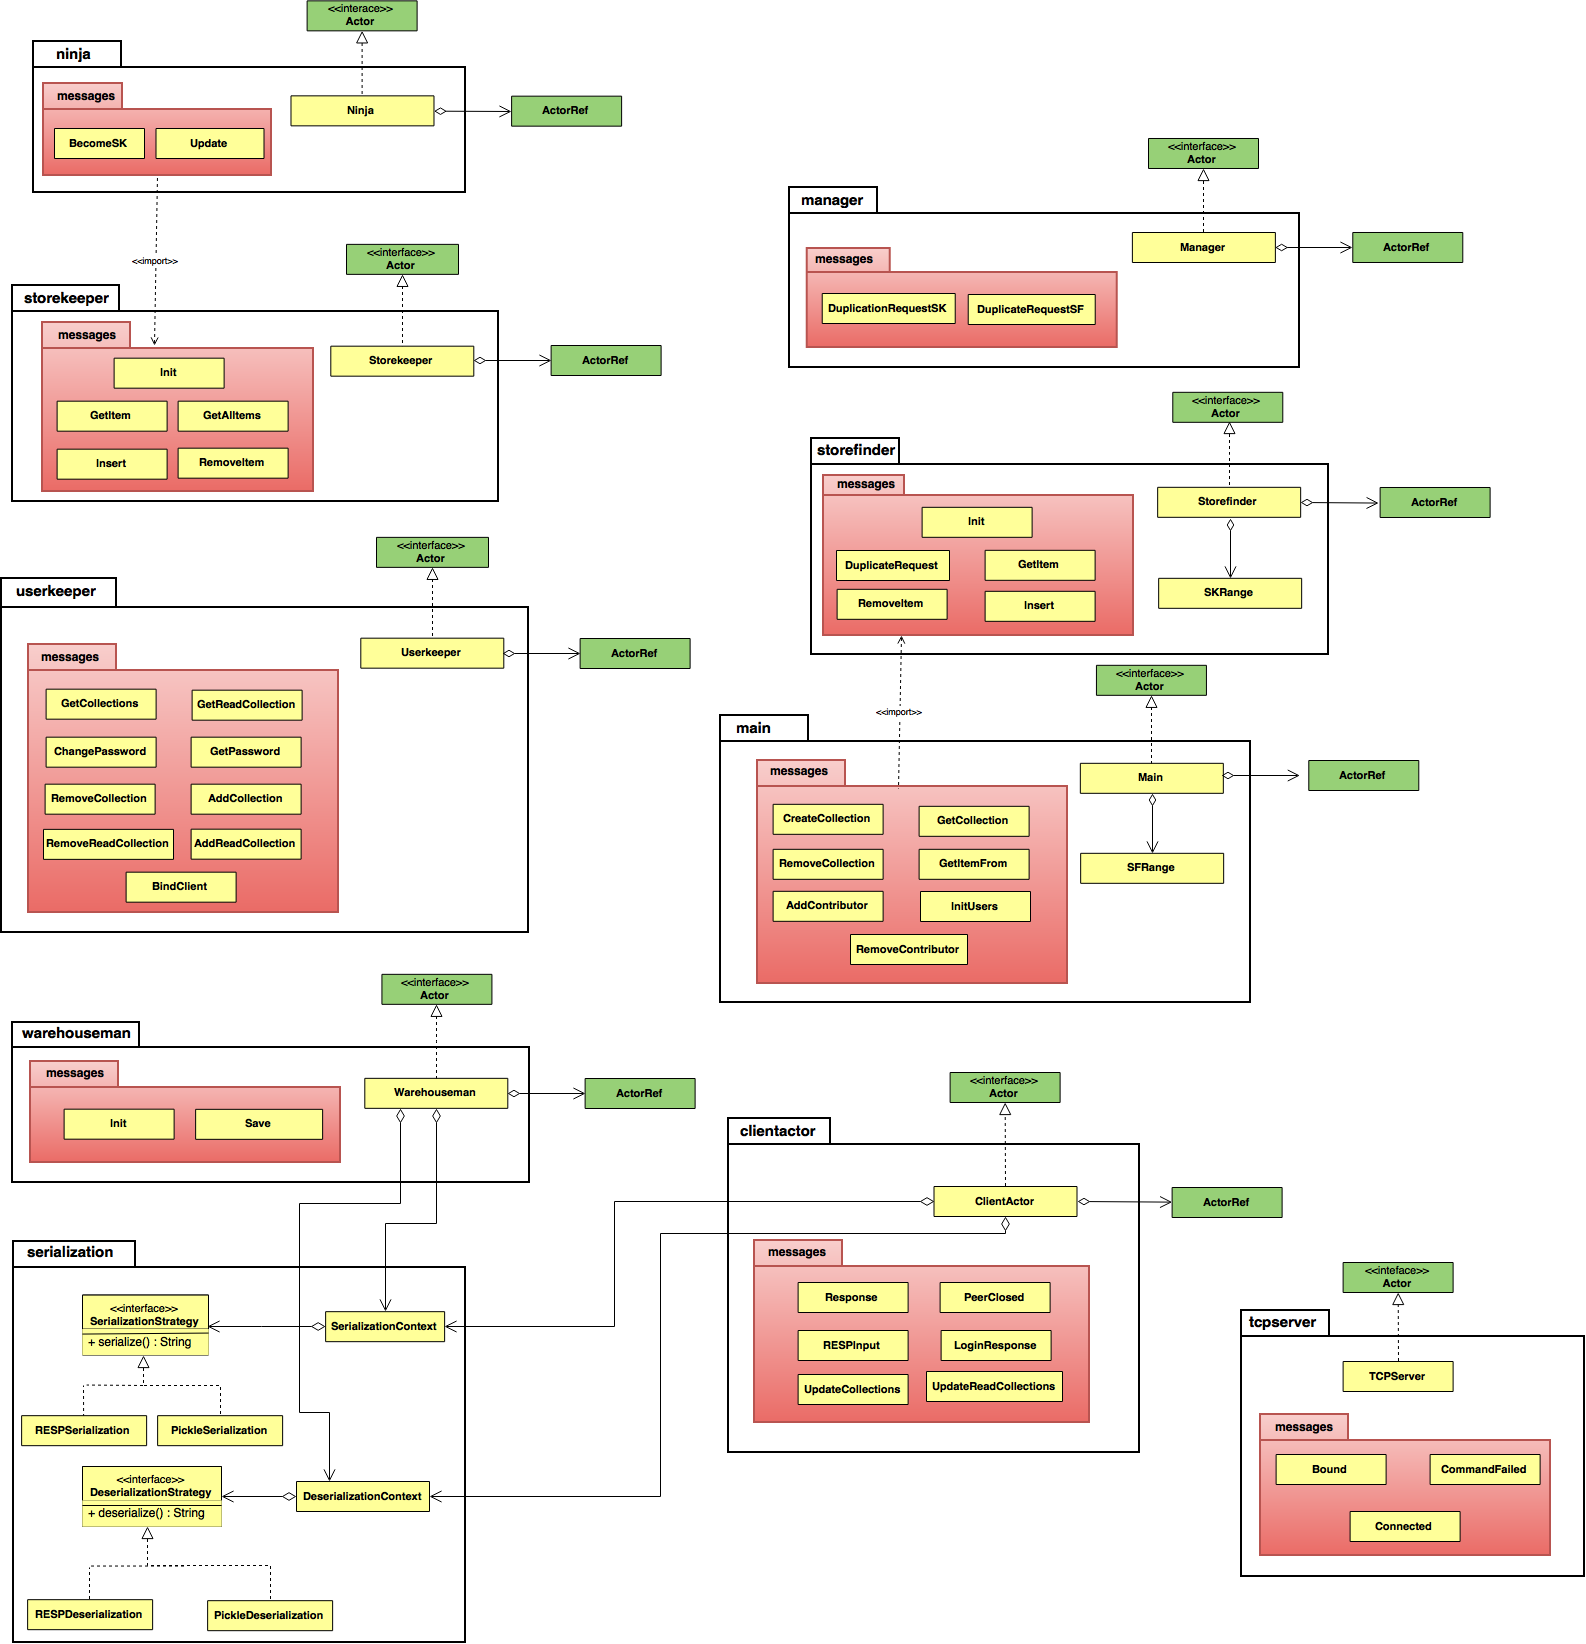
\includegraphics[width=1.1\textwidth,keepaspectratio]{RA/Actorsystem.png}
    \caption{\gloss{Package} actorsystem, visione generale}
  \end{center}
\end{figure}

\subsubsection{Descrizione}

\gloss{Package} che raggruppa tutte le componenti del sistema che
rappresentano il \gloss{server}.

\subsubsection{Package contenuti}

\begin{itemize}
\item \hyperref[sec:actorbase::actorsystem::actors]{actorbase::actorsystem::actors}
\item \hyperref[sec:actorbase::actorsystem::messages]{actorbase::actorsystem::messages}
\item \hyperref[sec:actorbase::actorsystem::utils]{actorbase::actorsystem::utils}.
\end{itemize}

\subsection{actorbase::actorsystem::utils}
\label{sec:actorbase::actorsystem::utils}

\begin{figure}[H]
  \begin{center}
    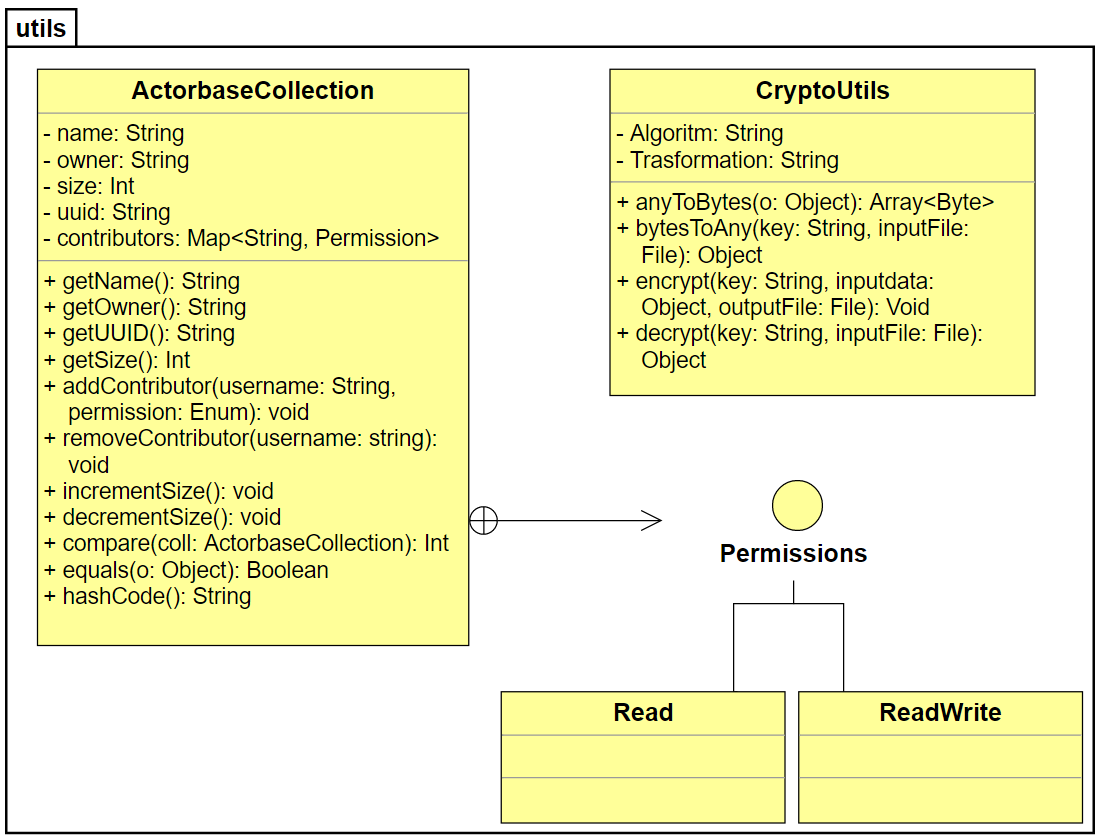
\includegraphics[width=0.8\textwidth,keepaspectratio]{RA/utils.png}
    \caption{Package actorsystem::utils}
  \end{center}
\end{figure}

\subsubsection{Descrizione}
\gloss{Package} contenente diverse classi di utilità.

\subsubsection{Interfacce}

\paragraph{Permissions}
\label{sec:actorbase::actorsystem::utils::Permissions}

\begin{figure}[H]
  \begin{center}
    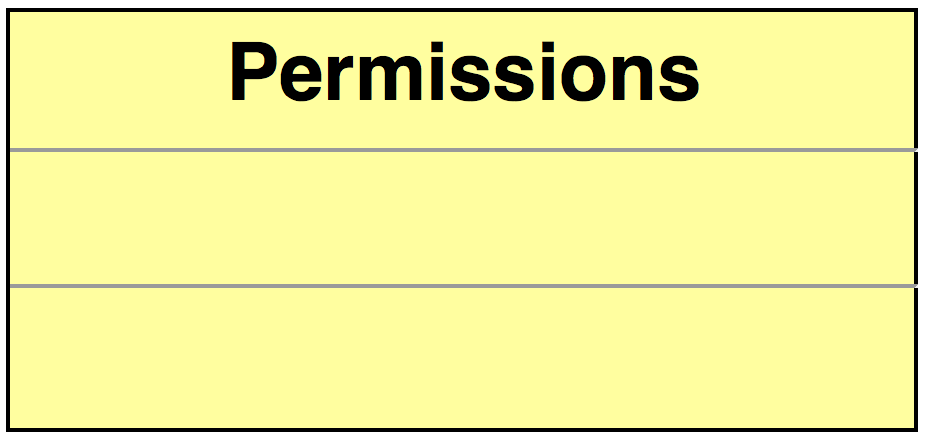
\includegraphics[width=0.2\textwidth,keepaspectratio]{RA/permissions.png}
    \caption{Classe actorsystem::utils::Permissions}
  \end{center}
\end{figure}

\subparagraph{Descrizione}

Interfaccia che rappresenta i permessi sulle \gloss{collezioni} da applicare ai
\gloss{collaboratori}.

\subparagraph{Utilizzo}

Viene utilizzata per rappresentare i tipi di permessi sulle \gloss{collezioni}
da applicare ai \gloss{collaboratori}.

\subparagraph{Realizzata da}

\begin{itemize}
\item \hyperref[sec:actorbase::actorsystem::utils::Read]{actorbase::actorsystem::utils::Read};
\item \hyperref[sec:actorbase::actorsystem::utils::ReadWrite]{actorbase::actorsystem::utils::ReadWrite}.
\end{itemize}

\subsubsection{Classi}

%%%%%%%%%%%%%%%%%%%%%%%%%%%%%%%%%%%%%%%%%%%%%%%%%%%%%%%%%%%%%%%%%%%%%%%%%
%%%%%%%%%%%%%%%%%%%%%%%%%%%%%%%%%%%%%%%%%%%%%%%%%%%%%%%%%%%%%%%%%%%%%%%%%

\paragraph{Read}
\label{sec:actorbase::actorsystem::utils::Read}

\begin{figure}[H]
  \begin{center}
    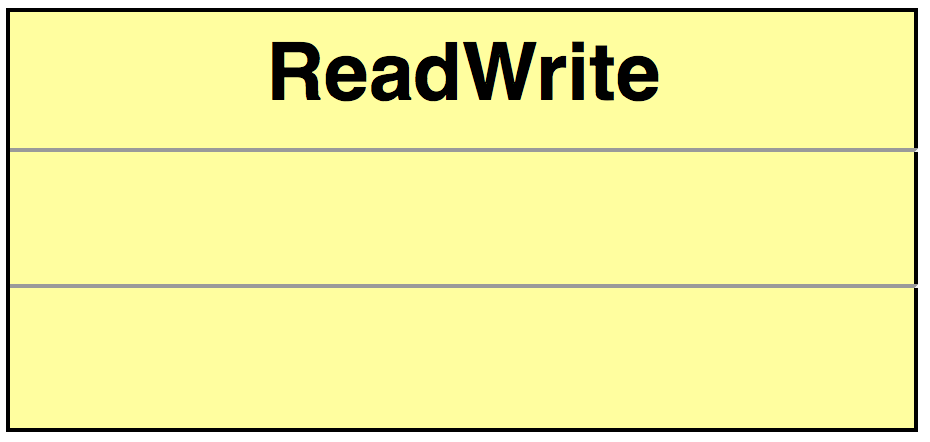
\includegraphics[width=0.2\textwidth,keepaspectratio]{RA/readWrite.png}
    \caption{Classe actorsystem::utils::Read}
  \end{center}
\end{figure}

\subparagraph{Descrizione}

Interfaccia che rappresenta i permessi di sola lettura sulle \gloss{collezioni}
da applicare ai \gloss{collaboratori}.

\subparagraph{Utilizzo}

Viene utilizzata per rappresentare i tipi di permessi di sola lettura sulle
\gloss{collezioni} da applicare ai \gloss{collaboratori}.

\subparagraph{Realizza}

\begin{itemize}
\item \hyperref[sec:actorbase::actorsystem::utils::Read]{actorbase::actorsystem::utils::Permissions}.
\end{itemize}

\paragraph{ReadWrite}
\label{sec:actorbase::actorsystem::utils::ReadWrite}

\begin{figure}[H]
  \begin{center}
    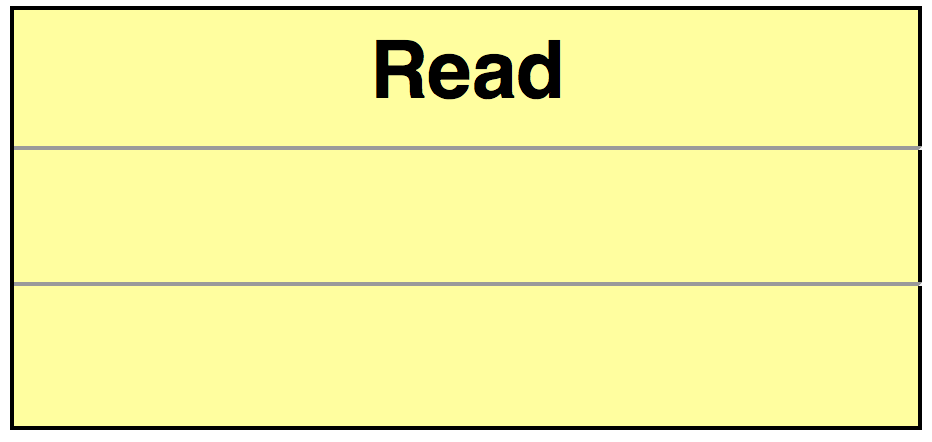
\includegraphics[width=0.2\textwidth,keepaspectratio]{RA/read.png}
    \caption{Classe actorsystem::utils::ReadWrite}
  \end{center}
\end{figure}

\subparagraph{Descrizione}

Interfaccia che rappresenta i permessi di lettura e scrittura sulle
\gloss{collezioni} da applicare ai \gloss{collaboratori}.

\subparagraph{Utilizzo}

Viene utilizzata per rappresentare i tipi di permessi di sola lettura e
scrittura sulle \gloss{collezioni} da applicare ai \gloss{collaboratori}.

\subparagraph{Realizza}

\begin{itemize}
\item \hyperref[sec:actorbase::actorsystem::utils::Read]{actorbase::actorsystem::utils::Permissions}.
\end{itemize}

\paragraph{CryptoUtils}
\label{sec:actorbase::actorsystem::utils::CryptoUtils}

\begin{figure}[H]
  \begin{center}
    \includegraphics[width=0.4\textwidth,keepaspectratio]{RA/cryptoutils.png}
    \caption{Classe actorsystem::utils::CryptoUtils}
  \end{center}
\end{figure}

\subparagraph{Descrizione}
Classe atta a criptare e decriptare i dati per il salvataggio e la lettura dei dati su disco, utilizzata
dagli attori di tipo \hyperref[sec:actorbase::actorsystem::actors::warehouseman::Warehouseman]{Warehouseman},
permette di impostare il tipo di crittografia da utilizzare.

\subparagraph{Utilizzo}
Viene utilizzata dall'attore di tipo \gloss{Warehouseman} per il salvataggio e la lettura del database su disco.

\subparagraph{Attributi}
\begin{tabular}{| p{3cm} | p{1.5cm} | p{2cm} | p{2cm} | p{8.5cm} |}
  \hline
  Nome & Accesso & Mutabilità & Tipo & Descrizione\\
  \hline
  Algorithm & privato & immutabile & String & Rappresenta l'algoritmo usato per la criptazione \\
  \hline
  Transformation & privato & immutabile & String & Rappresenta la trasformazione per ottenere il cifrario usato per la criptazione \\
  \hline
\end{tabular}

\subparagraph{Metodi}
\begin{tabular}{| p{3cm} | p{1.5cm} | p{3.5cm} | p{9cm} |}
  \hline
  Nome & Accesso & Tipo di ritorno & Descrizione\\
  \hline
  anyToBytes & pubblico & \gloss{Array} di \gloss{byte} & Metodo utilizzato per trasformare un oggetto qualsiasi in un \gloss{array} di \gloss{byte}\\
  \hline
  bytesToAny & pubblico & Object & Metodo utilizzato per riportare allo stato originale un oggetto rappresentato in forma \gloss{array} di \gloss{byte}\\
  \hline
  encrypt & pubblico & void & Metodo che si occupa di criptare i dati \\
  \hline
  decrypt<T> & pubblico & T & Metodo che si occupa di decriptare i dati riportandoli al tipo generico richiesto\\
  \hline
\end{tabular}

\subparagraph{Parametri}

\textbf{anyToBytes}\\ \\
\begin{tabular}{| l | l | l |}
  \hline
  Nome & Tipo & Descrizione\\
  \hline
  o & Object & Riferimento all'oggetto da trasformare in \gloss{array} di \gloss{byte}\\
  \hline
\end{tabular}\\

\textbf{bytesToAny}\\ \\
\begin{tabular}{| l | l | l |}
  \hline
  Nome & Tipo & Descrizione\\
  \hline
  key & String & Stringa che rappresenta la chiave di criptazione \\
  \hline
  inputFile & File & File che contiene i dati di persistenza del sistema criptati\\
  \hline
\end{tabular}\\

\textbf{encrypt}\\ \\
\begin{tabular}{| l | l | l |}
  \hline
  Nome & Tipo & Descrizione\\
  \hline
  key & String & Stringa che rappresenta la chiave di criptazione \\
  \hline
  inputData & Map<String, Object> & Mappa che rappresenta i dati che verranno criptati \\
  \hline
  outputFile & File & File destinato a contenere i dati criptati \\
  \hline
\end{tabular}\\

\textbf{decrypt<T>}\\
\begin{tabular}{| l | l | l |}
  \hline
  Nome & Tipo & Descrizione\\
  \hline
  key & String & Stringa che rappresenta la chiave di decriptazione \\
  \hline
  inputFile & File & File che contiene i dati da decriptare \\
  \hline
\end{tabular}\\

%%%%%%%%%%%%%%%%%%%%%%%%%%%%%%%%%%%%%%%%%%%%%%%%%%%%%%%%%%%%%%%%%%%%%%%%%%%%%%
%%%%%%%%%%%%%%%%%%%%%%%%%%%%%%%%%%%%%%%%%%%%%%%%%%%%%%%%%%%%%%%%%%%%%%%%%%%%%%

\paragraph{ActorbaseCollection}
\label{sec:actorbase::actorsystem::utils::ActorbaseCollection}

\begin{figure}[H]
  \begin{center}
    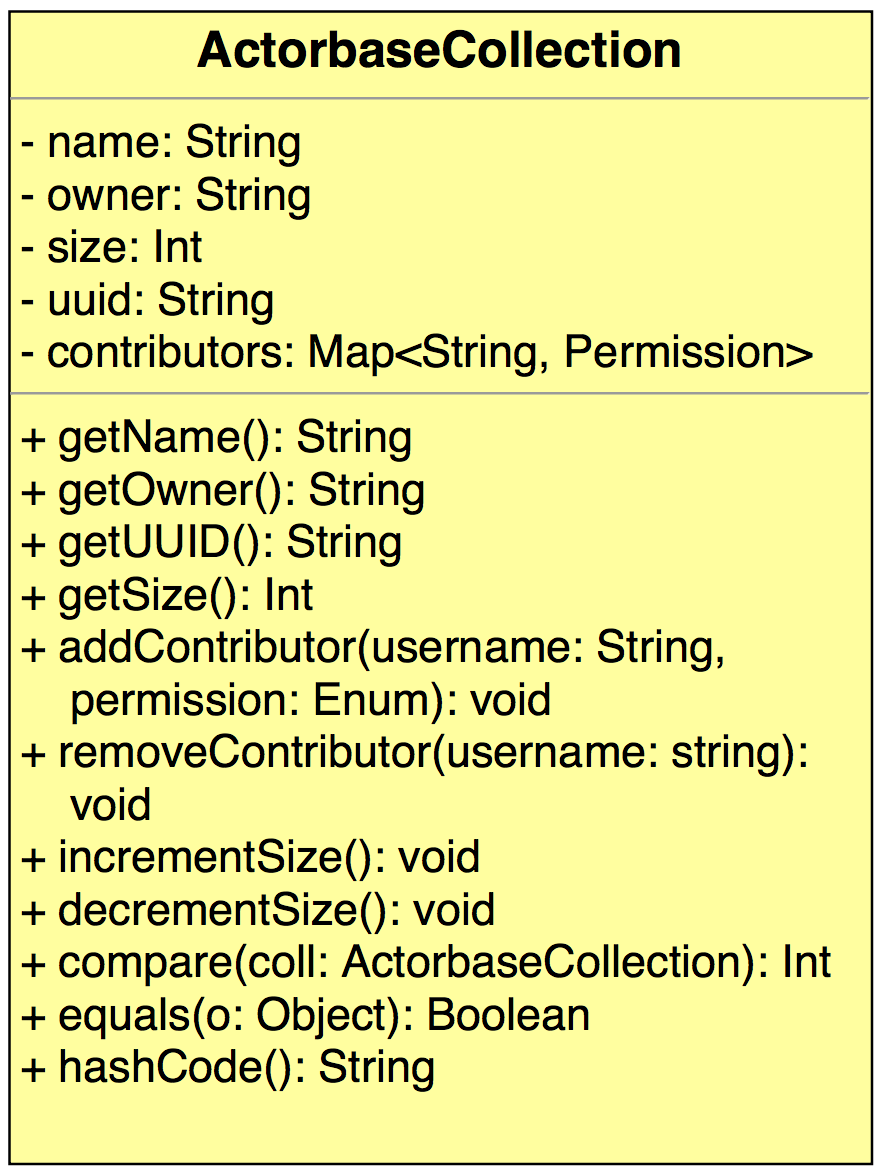
\includegraphics[width=0.4\textwidth,keepaspectratio]{RA/actorbaseCollectionUtils.png}
    \caption{Classe actorsystem::utils::ActorbaseCollection}
  \end{center}
\end{figure}

\subparagraph{Descrizione}
Classe atta a modellare una \gloss{collezione} del sistema actorbase.

\subparagraph{Utilizzo}
Viene utilizzata da diversi attori del sistema. Questa classe espone metodi
getter, metodi per aumentare e diminuire la dimensione della collezione
e un metodo per il confronto con un altro oggetto di questo tipo. Contiene
infine un identificativo univoco universale utilizzabile dall'estensione
\gloss{Akka} \textit{cluster sharding} per l'indirizzamento dei messaggi
riguardanti \gloss{collezioni}.

\subparagraph{Realizza}
\begin{itemize}
\item trait scala.math.Ordered
\end{itemize}

\subparagraph{Attributi}
\begin{tabular}{| p{3cm} | p{1.5cm} | p{2cm} | p{2cm} | p{8.5cm} |}
  \hline
  Nome & Accesso & Mutabilità & Tipo & Descrizione\\
  \hline
  name & privata & mutabile & String & Rappresenta il nome della \gloss{collezione} \\
  \hline
  owner & private & mutabile & String & Rappresenta lo username dell'utente che ha creato la \gloss{collezione} \\
  \hline
  uuid & private & immutabile & String & Rappresenta un identificativo univoco universale alla \gloss{collezione} all'interno del sistema\\
  \hline
  contributors & private & mutabile & Map<String, \hyperref[sec:actorbase::actorsystem::utils::Permissions]{Permissions}> & Rappresenta una mappa di \gloss{username} e permessi lettura o lettura-scrittura\\
  \hline
\end{tabular}

\subparagraph{Metodi}
\begin{tabular}{| p{3cm} | p{2cm} | p{3cm} | p{9cm} |}
  \hline
  Nome & Accesso & Tipo di ritorno & Descrizione\\
  \hline
  getName & pubblico & String & Metodo che ritorna il nome della \gloss{collezione} \\
  \hline
  getOwner & pubblico & String & Metodo che ritorna lo username dell'utente che ha creato la \gloss{collezione} \\
  \hline
  getSize & pubblico & Int & Metodo che ritorna la dimensione della \gloss{collezione} rappresentata\\
  \hline
  getUUID & pubblico & String & Metodo che ritorna lo uuid della collezione. Questo rappresenta una stringa per identificare univocamente diverse \gloss{collezioni}\\
  \hline
  addContributor & pubblico & void & Metodo che aggiunge un utente alla mappa dei \gloss{collaboratori} alla \gloss{collezione}\\
  \hline
  removeContributor & pubblico & void & Metodo che rimuove un utente alla mappa dei \gloss{collaboratori} alla \gloss{collezione}\\
  \hline
  incrementSize & pubblico & void & Metodo che incrementa di una unità la size della \gloss{collezione}. Usato quando si effettua un inserimento di un \gloss{item} \\
  \hline
  decrementSize & pubblico & void & Metodo che decrementa di una unità la size della \gloss{collezione}. Usato quando si effettua una rimozione di un \gloss{item} \\
  \hline
  compare & pubblico & Int & Metodo per l'implementazione dell'interfaccia Ordered. Permette di confrontare più oggetti ActorbaseCollection per capire se rappresentano la stessa \gloss{collezione}\\
  \hline
\end{tabular}

\subparagraph{Parametri}

\textbf{addContributor}\\ \\
\begin{tabular}{| l | l | l |}
  \hline
  Nome & Tipo & Descrizione\\
  \hline
  username & String & \gloss{Username} dell'utente da aggiungere alla mappa dei \gloss{collaboratori}\\
  \hline
\end{tabular}\\

\textbf{removeContributor}\\ \\
\begin{tabular}{| l | l | l |}
  \hline
  Nome & Tipo & Descrizione\\
  \hline
  username & String & \gloss{Username} dell'utente da rimuovere alla mappa dei \gloss{collaboratori}\\
  \hline
\end{tabular}\\

\textbf{compare}\\ \\
\begin{tabular}{| l | l | l |}
  \hline
  Nome & Tipo & Descrizione\\
  \hline
  that & \hyperref[sec:actorbase::actorsystem::utils::ActorbaseCollection]{ActorbaseCollection} & \hyperref[sec:actorbase::actorsystem::utils::ActorbaseCollection]{ActorbaseCollection} da confrontare con l'oggetto this \\
  \hline
\end{tabular}\\

%%%%%%%%%%%%%%%%%%%%%%%%%%%%%%%%%%%%%%%%%%%%%%%%%%%%%%%%%%%%%%%%%%%%%%%%%
%%%%%%%%%%%%%%%%%%%%%%%%%%%%%%%%%%%%%%%%%%%%%%%%%%%%%%%%%%%%%%%%%%%%%%%%%

\subsection{actorbase::actorsystem::messages}
\label{sec:actorbase::actorsystem::messages}

% TODO da aggiungere
\begin{figure}[H]
  \begin{center}
    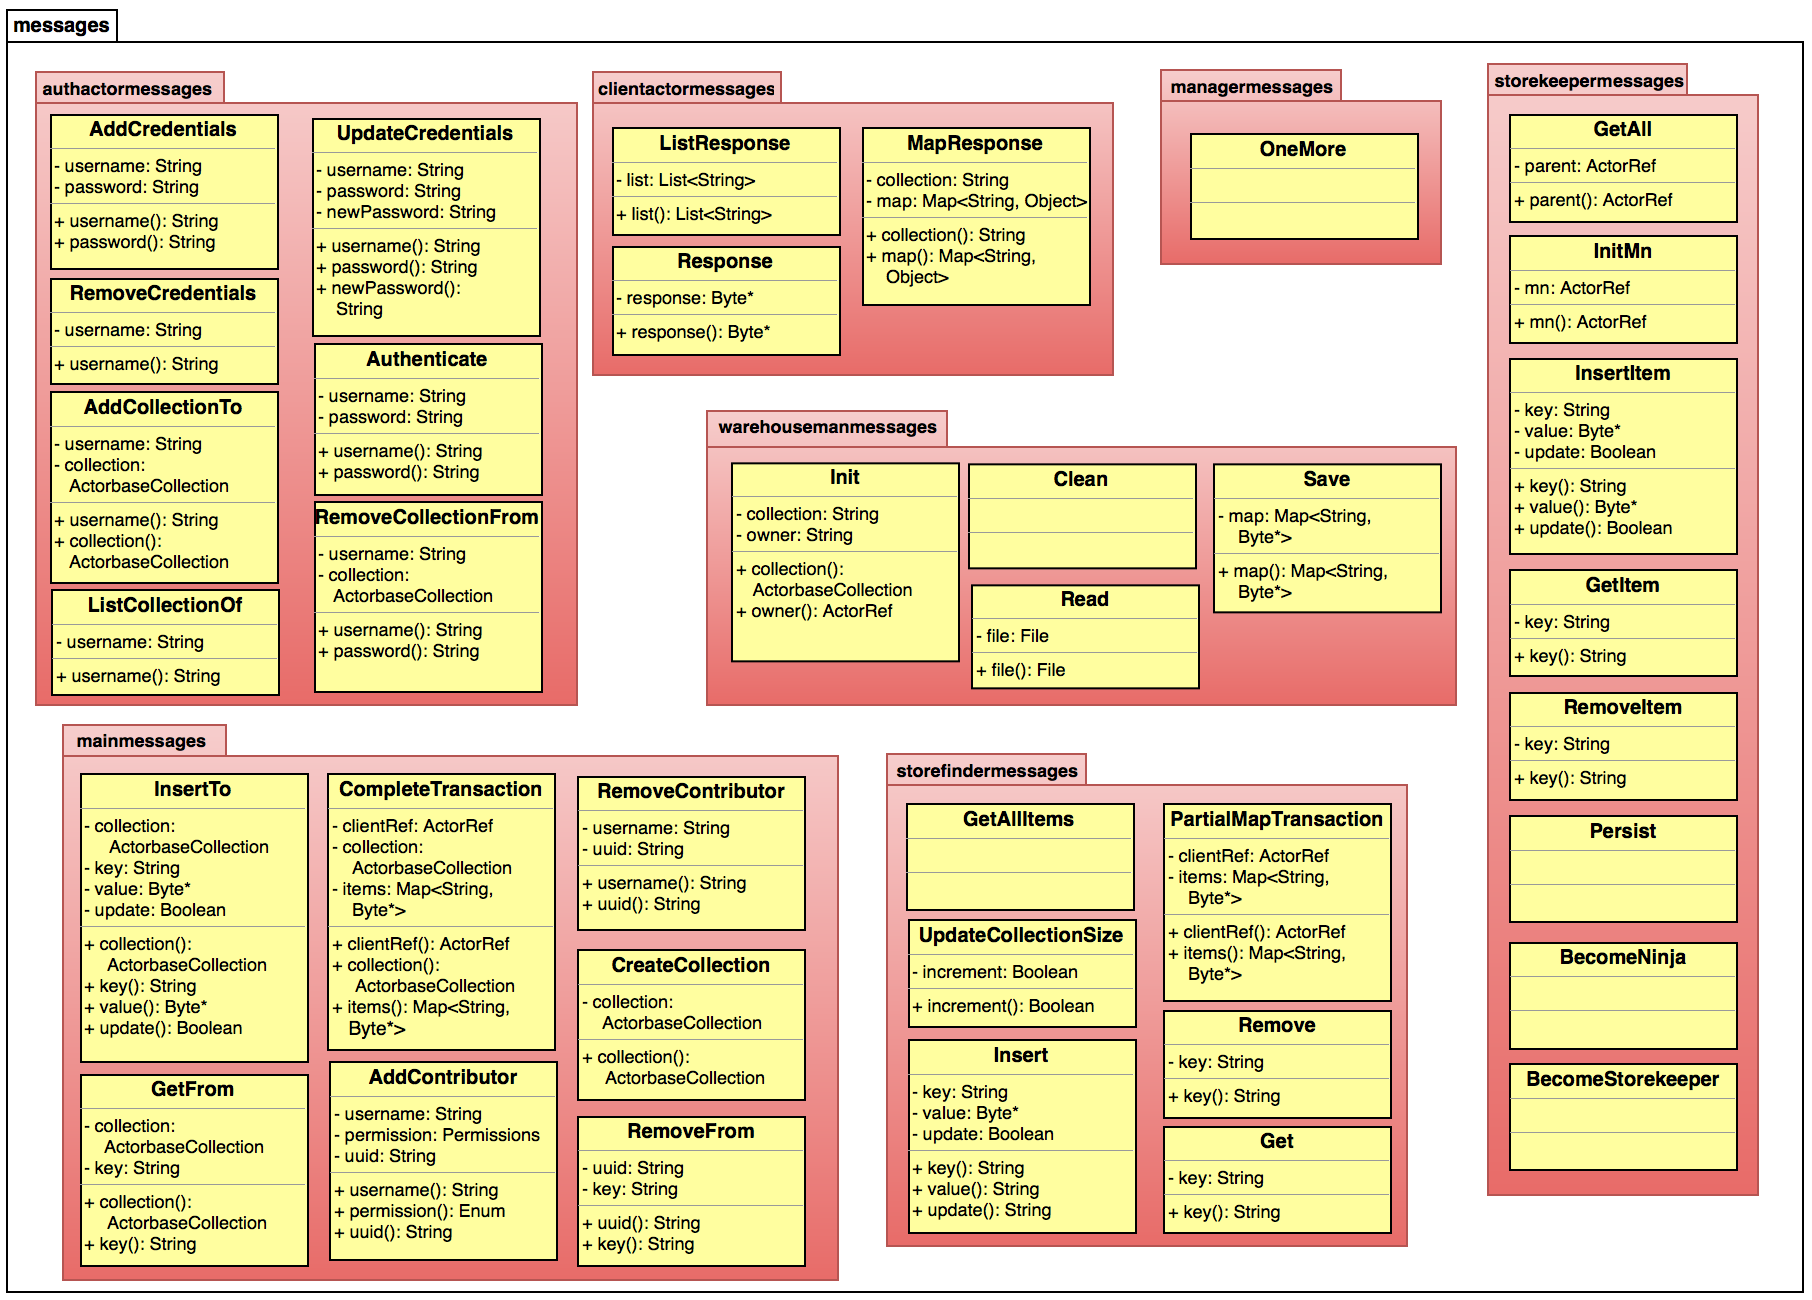
\includegraphics[width=1.0\textwidth,keepaspectratio]{RA/messages.png}
    \caption{\gloss{Package} messages}
  \end{center}
\end{figure}

\subsubsection{Descrizione}

\gloss{Package} che raggruppa tutti i messaggi del \gloss{server}.

\subsubsection{Package contenuti}

\begin{itemize}
\item \hyperref[sec:actorbase::actorsystem::messages::authactormessages]{actorbase::actorsystem::messages::authactormessages};
\item \hyperref[sec:actorbase::actorsystem::messages::clientactormessages]{actorbase::actorsystem::messages::clientactormessages};
\item \hyperref[sec:actorbase::actorsystem::messages::mainmessages]{actorbase::actorsystem::messages::mainmessages};
\item \hyperref[sec:actorbase::actorsystem::messages::storefindermessages]{actorbase::actorsystem::messages::storefindermessages};
\item \hyperref[sec:actorbase::actorsystem::messages::storekeepermessages]{actorbase::actorsystem::messages::storekeepermessages};
\item \hyperref[sec:actorbase::actorsystem::messages::warehousemanmessages]{actorbase::actorsystem::messages::warehousemanmessages};
\item \hyperref[sec:actorbase::actorsystem::messages::warehousemanmessages]{actorbase::actorsystem::messages::manangermessages}.
\end{itemize}

\subsection{actorbase::actorsystem::messages::authactormessages}
\label{sec:actorbase::actorsystem::messages::authactormessages}

% TODO img
\begin{figure}[H]
  \begin{center}
    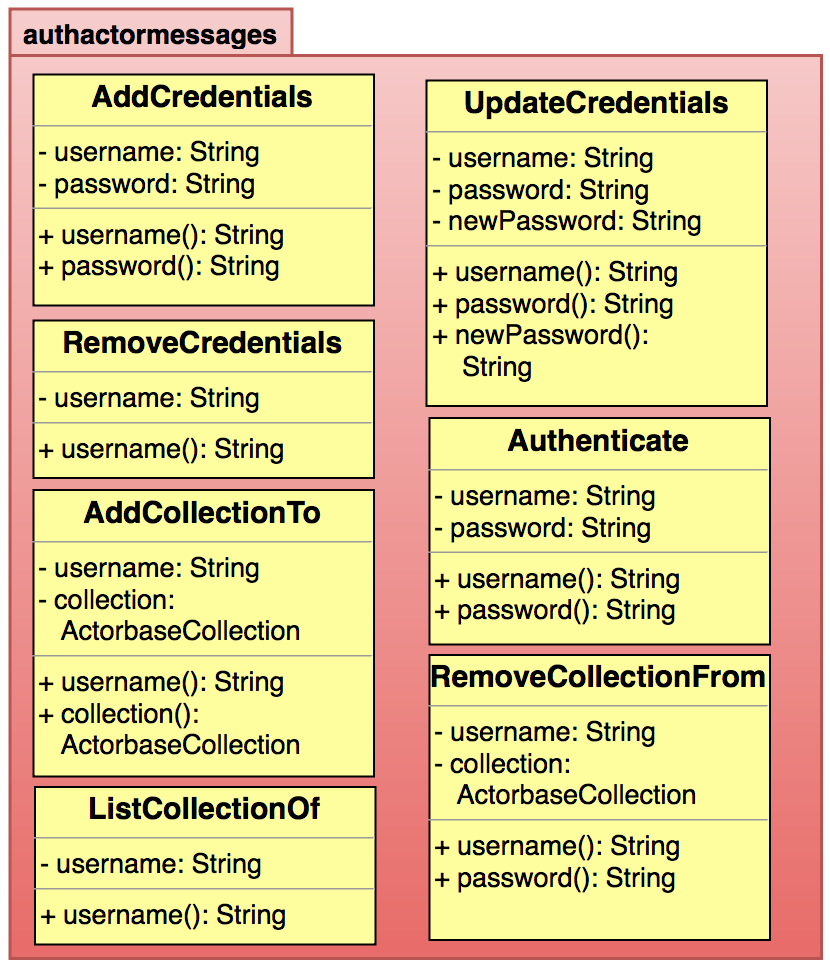
\includegraphics[width=0.6\textwidth,keepaspectratio]{RA/authactormessages.png}
    \caption{Package actorsystem::messages::authactormessages}
  \end{center}
\end{figure}

\subsubsection{Descrizione}
\gloss{Package} contenente i messaggi processabili dall'attore \hyperref[sec:actorbase::actorsystem::actors::authactor::AuthActor]{AuthActor}.

\subsubsection{Classi}

\paragraph{actorbase::actorsystem::messages::authactormessages::AddCredentials}
\label{sec:actorbase::actorsystem::messages::authactormessages::AddCredentials}

% TODO img
\begin{figure}[H]
  \begin{center}
    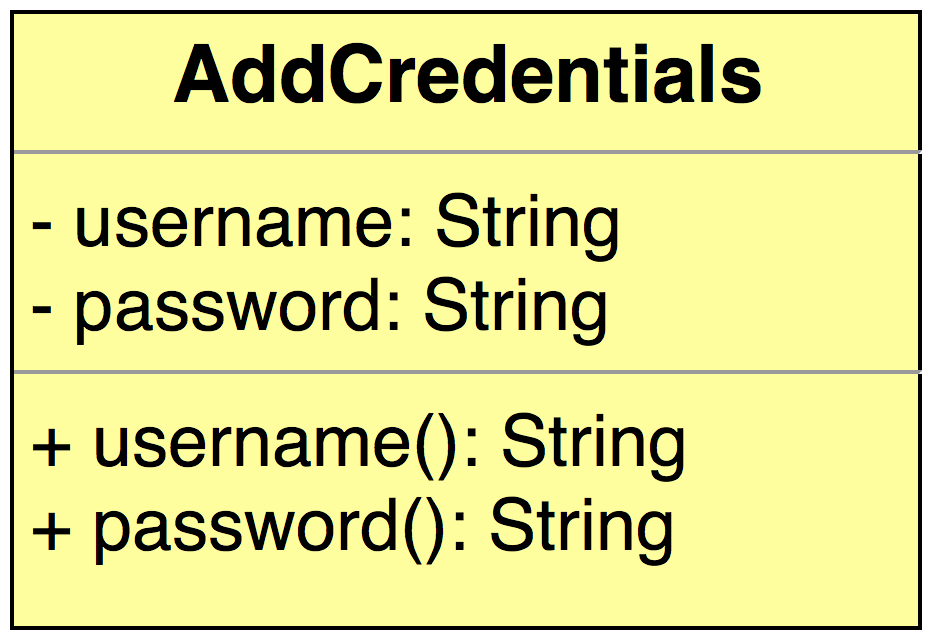
\includegraphics[width=0.3\textwidth,keepaspectratio]{RA/addCredentials.png}
    \caption{Classe AddCredentials}
  \end{center}
\end{figure}

\subparagraph{Descrizione}
Classe che rappresenta una richiesta di aggiunta di credenziali al
sistema.\\Implementata utilizzando la specifica funzionalità \textit{case class}
di \gloss{Scala}, in modo da poter usufruirne mediante costrutti e algoritmi di
\gloss{pattern matching}.

\subparagraph{Utilizzo}
Questa classe viene utilizzata per mandare una richiesta all'\gloss{attore}
\hyperref[sec:actorbase::actorsystem::messages::authactormessages::AuthActor]{AuthActor}
di aggiunta di credenziali al sistema, all'interno del metodo \textit{Receive} che la utilizza
avviene inoltre il controllo della password, in modo che rispetti i vincoli imposti dal sistema.

\subparagraph{Attributi}
\begin{tabular}{| p{2cm} | p{1.5cm} | p{2cm} | p{3cm} | p{8.5cm} |}
  \hline
  Nome & Accesso & Mutabilità & Tipo & Descrizione\\
  \hline
  username & privato & immutabile & String & Rappresenta lo username da aggiungere alle credenziali del sistema \\
  \hline
  password & privato & immutabile & String & Rappresenta la password da aggiungere abbinata dallo username aggiunto \\
  \hline
\end{tabular}

\subparagraph{Metodi}
\begin{tabular}{| p{3cm} | p{1.5cm} | p{3.5cm} | p{9cm} |}
  \hline
  Nome & Accesso & Tipo di ritorno & Descrizione\\
  \hline
  username & pubblico & String & Metodo che ritorna l'attributo \gloss{username}\\
  \hline
  password & pubblico & String & Metodo che ritorna l'attributo \gloss{password}\\
  \hline
\end{tabular}

\paragraph{actorbase::actorsystem::messages::authactormessages::UpdateCredentials}
\label{sec:actorbase::actorsystem::messages::authactormessages::UpdateCredentials}

% TODO img
\begin{figure}[H]
  \begin{center}
    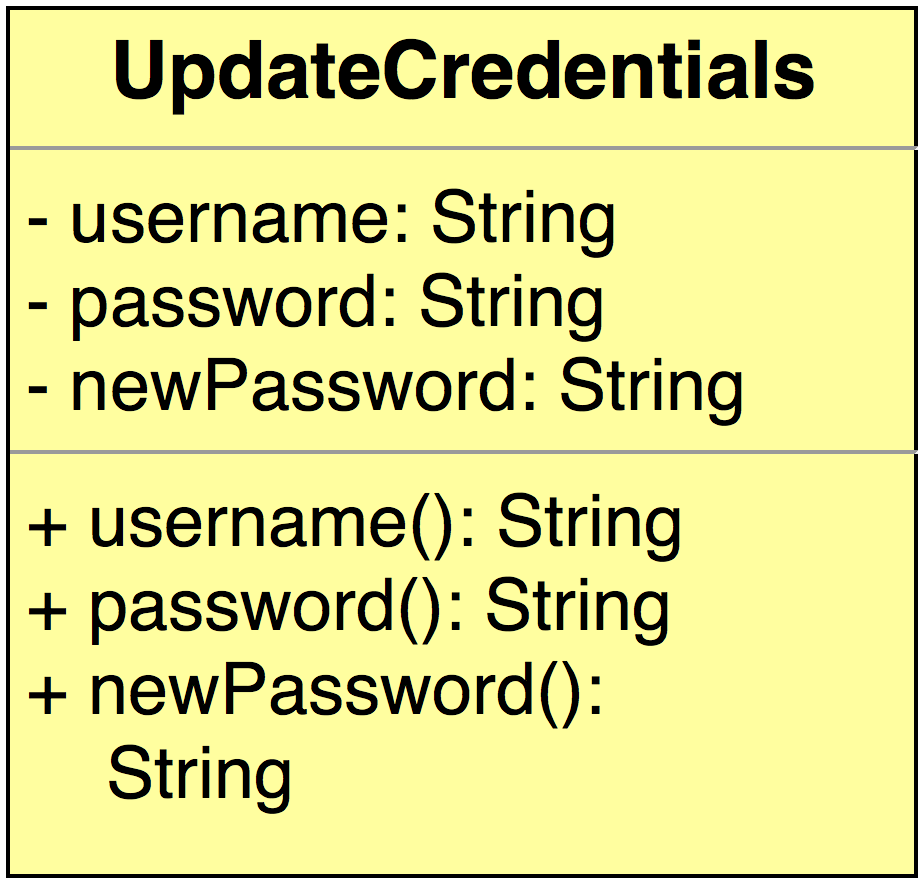
\includegraphics[width=0.3\textwidth,keepaspectratio]{RA/updateCredentials.png}
    \caption{Classe UpdateCredentials}
  \end{center}
\end{figure}

\subparagraph{Descrizione}
Classe che rappresenta una richiesta di modifica di password di un utente al
sistema.\\Implementata utilizzando la specifica funzionalità \textit{case class}
di \gloss{Scala}, in modo da poter usufruirne mediante costrutti e algoritmi di
\gloss{pattern matching}.

\subparagraph{Utilizzo}
Questa classe viene utilizzata per mandare una richiesta all'attore
\hyperref[sec:actorbase::actorsystem::actors::authactormessages::AuthActor]{AuthActor}
di modifica della password di un utente.

\subparagraph{Attributi}
\begin{tabular}{| p{2cm} | p{1.5cm} | p{2cm} | p{3cm} | p{8.5cm} |}
  \hline
  Nome & Accesso & Mutabilità & Tipo & Descrizione\\
  \hline
  username & privato & immutabile & String & Rappresenta lo \gloss{username} dell'utente a cui cambiare la \gloss{password} \\
  \hline
  password & privato & immutabile & String & Rappresenta la vecchia \gloss{password} da cambiare \\
  \hline
  newPassword & privato & immutabile & String & Rappresenta la nuova password da assegnare all'utente rappresentato dallo \gloss{username} immesso \\
  \hline
\end{tabular}

\subparagraph{Metodi}
\begin{tabular}{| p{3cm} | p{1.5cm} | p{3.5cm} | p{9cm} |}
  \hline
  Nome & Accesso & Tipo di ritorno & Descrizione\\
  \hline
  username & pubblico & String & Metodo che ritorna l'attributo username\\
  \hline
  password & pubblico & String & Metodo che ritorna l'attributo password\\
  \hline
  newPassword & pubblico & String & Metodo che ritorna l'attributo newPassword\\
  \hline
\end{tabular}

\paragraph{actorbase::actorsystem::messages::authactormessages::RemoveCredentials}
\label{sec:actorbase::actorsystem::messages::authactormessages::RemoveCredentials}

% TODO img
\begin{figure}[H]
  \begin{center}
    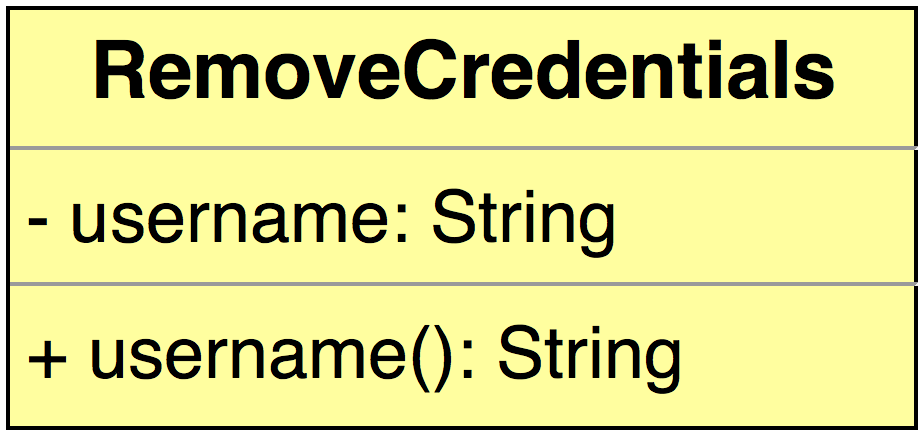
\includegraphics[width=0.3\textwidth,keepaspectratio]{RA/removeCredentials.png}
    \caption{Classe RemoveCredentials}
  \end{center}
\end{figure}

\subparagraph{Descrizione}
Classe che rappresenta una richiesta di rimozione di un utente dal
sistema.\\Implementata utilizzando la specifica funzionalità \textit{case class}
di \gloss{Scala}, in modo da poter usufruirne mediante costrutti e algoritmi di
\gloss{pattern matching}.

\subparagraph{Utilizzo}
Questa classe viene utilizzata per mandare una richiesta all'\gloss{attore}
\hyperref[sec:actorbase::actorsystem::actors::authactor::AuthActor]{AuthActor}
di rimozione di un utente.

\subparagraph{Attributi}
\begin{tabular}{| p{2cm} | p{1.5cm} | p{2cm} | p{3cm} | p{8.5cm} |}
  \hline
  Nome & Accesso & Mutabilità & Tipo & Descrizione\\
  \hline
  username & privato & immutabile & String & Rappresenta lo username dell'utente da rimuovere dal sistema\\
  \hline
\end{tabular}

\subparagraph{Metodi}
\begin{tabular}{| p{3cm} | p{1.5cm} | p{3.5cm} | p{9cm} |}
  \hline
  Nome & Accesso & Tipo di ritorno & Descrizione\\
  \hline
  username & pubblico & String & Metodo che ritorna l'attributo username\\
  \hline
\end{tabular}

\paragraph{actorbase::actorsystem::messages::authactormessages::Authenticate}
\label{sec:actorbase::actorsystem::messages::authactormessages::Authenticate}

% TODO img
\begin{figure}[H]
  \begin{center}
    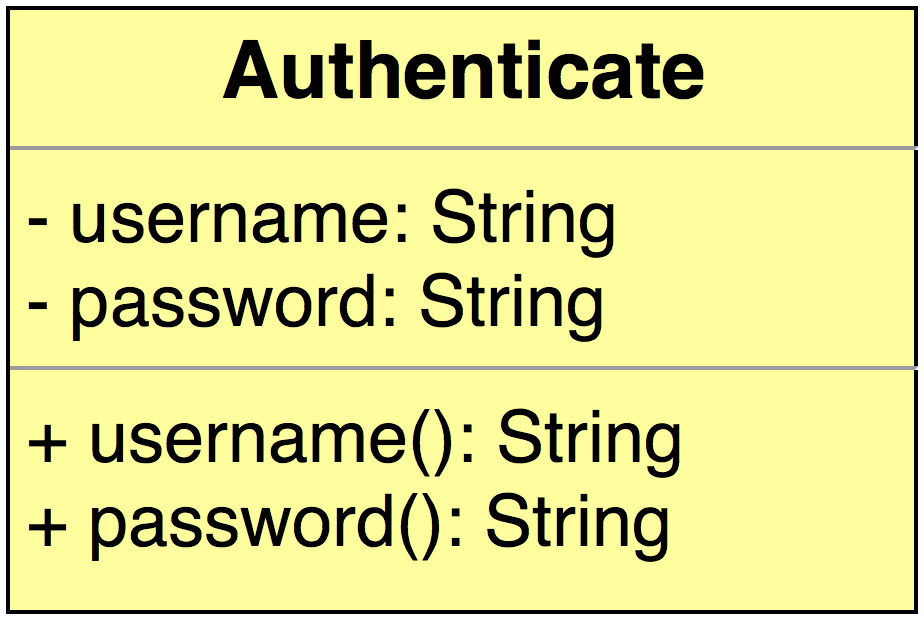
\includegraphics[width=0.3\textwidth,keepaspectratio]{RA/Authenticate.png}
    \caption{Classe Authenticate}
  \end{center}
\end{figure}

\subparagraph{Descrizione}
Classe che rappresenta una richiesta di login di un utente al sistema.\\Implementata utilizzando la specifica funzionalità \textit{case class} di Scala,
in modo da poter usufruirne mediante costrutti e algoritmi di
\gloss{pattern matching}.

\subparagraph{Utilizzo}
Questa classe viene utilizzata per mandare una richiesta all'attore
\hyperref[sec:actorbase::actorsystem::actors::authactor::AuthActor]{AuthActor}
di accesso al sistema. L'attore \hyperref[sec:actorbase::actorsystem::actors::authactor::AuthActor]{AuthActor}
dovrà controllare se le credenziali immesse dall'utente sono corrette.

\subparagraph{Attributi}
\begin{tabular}{| p{2cm} | p{1.5cm} | p{2cm} | p{3cm} | p{8.5cm} |}
  \hline
  Nome & Accesso & Mutabilità & Tipo & Descrizione\\
  \hline
  username & privato & immutabile & String & Rappresenta lo username dell'utente che vuole effettuare il login \\
  \hline
  password & privato & immutabile & String & Rappresenta la password dell'utente che vuole effettuare il login \\
  \hline
\end{tabular}

\subparagraph{Metodi}
\begin{tabular}{| p{3cm} | p{1.5cm} | p{3.5cm} | p{9cm} |}
  \hline
  Nome & Accesso & Tipo di ritorno & Descrizione\\
  \hline
  username & pubblico & String & Metodo che ritorna l'attributo username\\
  \hline
  password & pubblico & String & Metodo che ritorna l'attributo password\\
  \hline
\end{tabular}

\paragraph{actorbase::actorsystem::messages::authactormessages::AddCollectionTo}
\label{sec:actorbase::actorsystem::messages::authactormessages::AddCollectionTo}

% TODO img
\begin{figure}[H]
  \begin{center}
    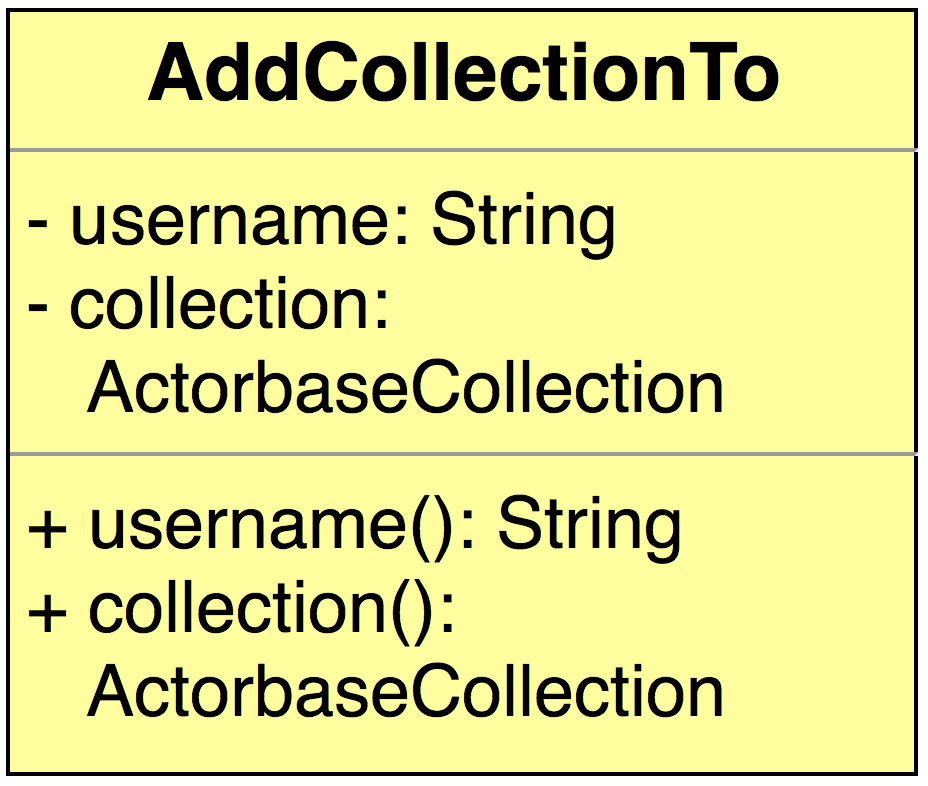
\includegraphics[width=0.3\textwidth,keepaspectratio]{RA/addCollectionTo.png}
    \caption{Classe AddCollectionTo}
  \end{center}
\end{figure}

\subparagraph{Descrizione}
Classe che rappresenta una richiesta di inserimento di una \gloss{collezione} ad
uno specifico utente del sistema.\\ Implementata utilizzando la specifica
funzionalità \textit{case class} di Scala, in modo da poter usufruirne mediante
costrutti e algoritmi di \gloss{pattern matching}.

\subparagraph{Utilizzo}
Questa classe viene utilizzata per mandare una richiesta all'attore
\hyperref[sec:actorbase::actorsystem::actors::authactor::AuthActor]{AuthActor}
di inserimento nuova \gloss{collezione} all'utente specificato. L'attore
\hyperref[sec:actorbase::actorsystem::actors::authactor::AuthActor]{AuthActor}
dovrà controllare che l'utente a cui aggiungere la \gloss{collezione} sia
presente nel sistema e che la \gloss{collezione} da inserire non sia già
presente associata all'utente stesso.

\subparagraph{Attributi}
\begin{tabular}{| p{2cm} | p{1.5cm} | p{2cm} | p{3cm} | p{8.5cm} |}
  \hline
  Nome & Accesso & Mutabilità & Tipo & Descrizione\\
  \hline
  username & privato & immutabile & String & Rappresenta lo username dell'utente a cui aggiungere la nuova \gloss{collezione}\\
  \hline
  collection & privato & immutabile & \hyperref[sec:actorbase::actorsystem::utils::ActorbaseCollection]{ActorbaseCollection} & Rappresenta la \gloss{collezione} da aggiungere alla lista associata all'utente specificato\\
  \hline
\end{tabular}

\subparagraph{Metodi}
\begin{tabular}{| p{3cm} | p{1.5cm} | p{3.5cm} | p{9cm} |}
  \hline
  Nome & Accesso & Tipo di ritorno & Descrizione\\
  \hline
  username & pubblico & String & Metodo di accesso in sola lettura che ritorna l'attributo username\\
  \hline
  collection & pubblico & \hyperref[sec:actorbase::actorsystem::utils::ActorbaseCollection]{ActorbaseCollection} & Metodo di accesso in sola lettura che ritorna l'attributo collection\\
  \hline
\end{tabular}

\paragraph{actorbase::actorsystem::messages::authactormessages::RemoveCollectionFrom}
\label{sec:actorbase::actorsystem::messages::authactormessages::RemoveCollectionFrom}

% TODO img
\begin{figure}[H]
  \begin{center}
    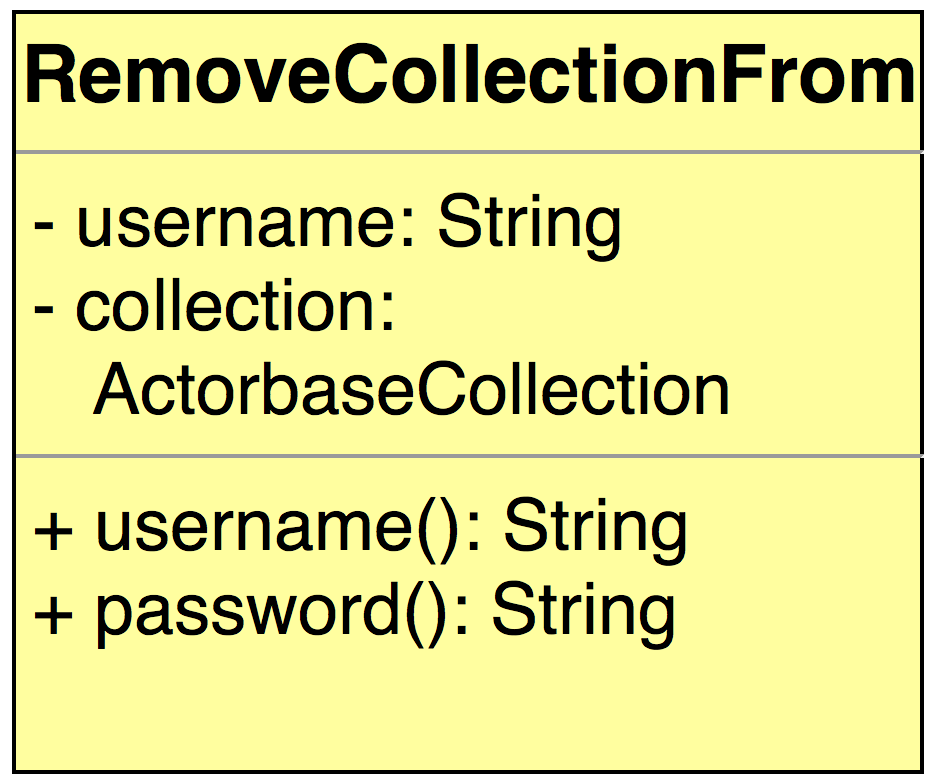
\includegraphics[width=0.3\textwidth,keepaspectratio]{RA/removeCollectionFrom.png}
    \caption{Classe RemoveCollectionFrom}
  \end{center}
\end{figure}

\subparagraph{Descrizione}
Classe che rappresenta una richiesta di rimozione di una \gloss{collezione}
associata ad uno specifico utente del sistema.\\ Implementata utilizzando la
specifica funzionalità \textit{case class} di Scala, in modo da poter usufruirne
mediante costrutti e algoritmi di \gloss{pattern matching}.

\subparagraph{Utilizzo}
Questa classe viene utilizzata per mandare una richiesta all'attore
\hyperref[sec:actorbase::actorsystem::actors::authactor::AuthActor]{AuthActor}
di rimozione di una \gloss{collezione} associata all'utente specificato.
L'attore
\hyperref[sec:actorbase::actorsystem::actors::authactor::AuthActor]{AuthActor}
dovrà controllare che l'utente a cui rimuovere la \gloss{collezione} sia
presente nel sistema e che la \gloss{collezione} da rimuovere sia effettivamente
presente e associata all'utente stesso.

\subparagraph{Attributi}
\begin{tabular}{| p{2cm} | p{1.5cm} | p{2cm} | p{3cm} | p{8.5cm} |}
  \hline
  Nome & Accesso & Mutabilità & Tipo & Descrizione\\
  \hline
  username & privato & immutabile & String & Rappresenta lo username dell'utente a cui rimuovere la \gloss{collezione} specificata\\
  \hline
  collection & privato & immutabile & \hyperref[sec:actorbase::actorsystem::utils::ActorbaseCollection]{ActorbaseCollection} & Rappresenta la \gloss{collezione} da rimuovere  dalla lista associata all'utente specificato\\
  \hline
\end{tabular}

\subparagraph{Metodi}
\begin{tabular}{| p{3cm} | p{1.5cm} | p{3.5cm} | p{9cm} |}
  \hline
  Nome & Accesso & Tipo di ritorno & Descrizione\\
  \hline
  username & pubblico & String & Metodo di accesso in sola lettura che ritorna l'attributo username\\
  \hline
  collection & pubblico & \hyperref[sec:actorbase::actorsystem::utils::ActorbaseCollection]{ActorbaseCollection} & Metodo di accesso in sola lettura che ritorna l'attributo collection\\
  \hline
\end{tabular}

\paragraph{actorbase::actorsystem::messages::authactormessages::ListCollectionsOf}
\label{sec:actorbase::actorsystem::messages::authactormessages::ListCollectionsOf}

% TODO img
\begin{figure}[H]
  \begin{center}
    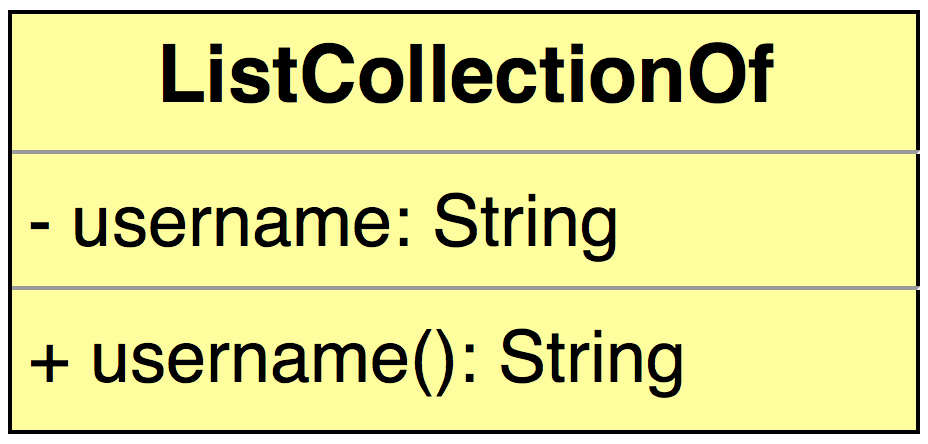
\includegraphics[width=0.3\textwidth,keepaspectratio]{RA/ListCollectionsOf.png}
    \caption{Classe ListCollectionsOf}
  \end{center}
\end{figure}

\subparagraph{Descrizione}
Classe che rappresenta una richiesta di visualizzazione delle \gloss{collezioni}
associate ad uno specifico utente del sistema.\\ Implementata utilizzando la
specifica funzionalità \textit{case class} di Scala, in modo da poter usufruirne
mediante costrutti e algoritmi di \gloss{pattern matching}.

\subparagraph{Utilizzo}
Questa classe viene utilizzata per mandare una richiesta all'attore
\hyperref[sec:actorbase::actorsystem::actors::authactor::AuthActor]{AuthActor}
di visualizzazione delle \gloss{collezioni} associate all'utente specificato.
L'attore
\hyperref[sec:actorbase::actorsystem::actors::authactor::AuthActor]{AuthActor}
dovrà controllare che l'utente specificato sia presente nel sistema.

\subparagraph{Attributi}
\begin{tabular}{| p{2cm} | p{1.5cm} | p{2cm} | p{3cm} | p{8.5cm} |}
  \hline
  Nome & Accesso & Mutabilità & Tipo & Descrizione\\
  \hline
  username & privato & immutabile & String & Rappresenta lo \gloss{username} dell'utente di cui si vuole visualizzare la lista \gloss{collezioni} create o a cui contribuisce\\
  \hline
\end{tabular}

\subparagraph{Metodi}
\begin{tabular}{| p{3cm} | p{1.5cm} | p{3.5cm} | p{9cm} |}
  \hline
  Nome & Accesso & Tipo di ritorno & Descrizione\\
  \hline
  username & pubblico & String & Metodo di accesso in sola lettura che ritorna l'attributo \gloss{username}\\
  \hline
\end{tabular}

%%%%%%%%%%%%%%%%%%%%%%%%%%%%%%%%%%%%%%%%%%%%%%%%%%%%%%%%%%%%%%%%%%%%%%%%%

\subsection{actorbase::actorsystem::messages::clientactormessages}
\label{sec:actorbase::actorsystem::messages::clientactormessages}

% TODO img
\begin{figure}[H]
  \begin{center}
    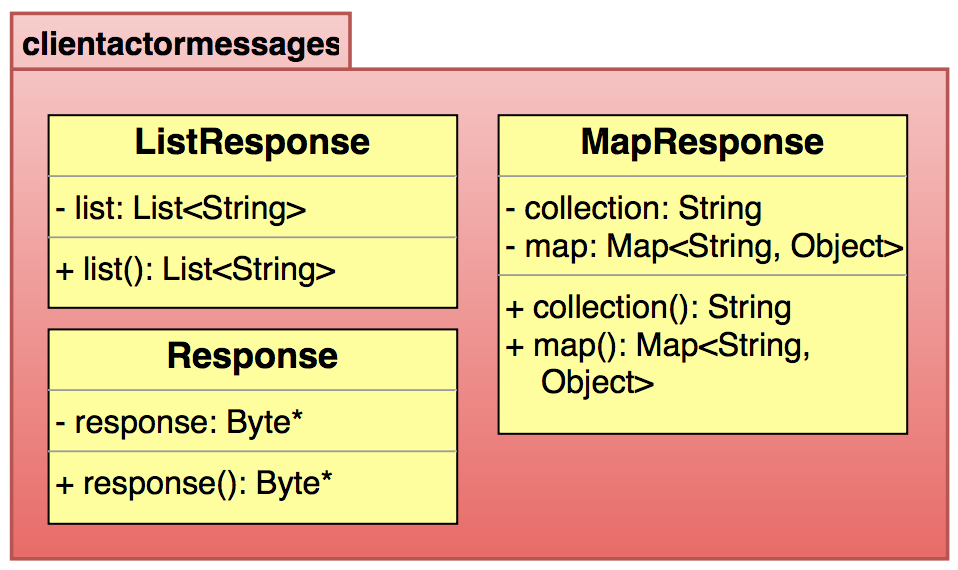
\includegraphics[width=0.7\textwidth,keepaspectratio]{RA/clientactormessages.png}
    \caption{Package actorsystem::messages::clientactormessages}
  \end{center}
\end{figure}

\subsubsection{Descrizione}
\gloss{Package} contenente i messaggi processabili dall'attore \hyperref[sec:actorbase::actorsystem::actors::clientactor::ClientActor]{ClientActor}.

\subsubsection{Classi}

\paragraph{actorbase::actorsystem::messages::clientactormessages::ListResponse}
\label{sec:actorbase::actorsystem::messages::clientactormessages::ListResponse}

% TODO img
\begin{figure}[H]
  \begin{center}
    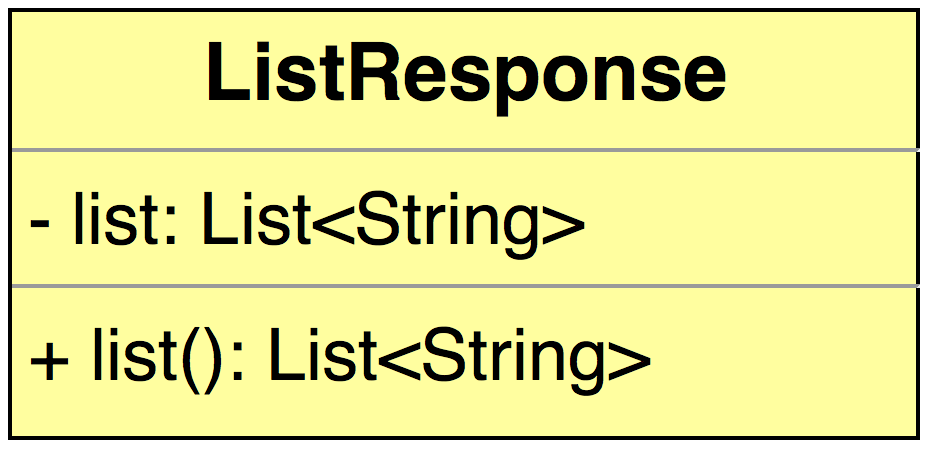
\includegraphics[width=0.3\textwidth,keepaspectratio]{RA/listResponse.png}
    \caption{Classe ListResponse}
  \end{center}
\end{figure}

\subparagraph{Descrizione}
Classe che rappresenta un messaggio utilizzato per consegnare al
\hyperref[sec:actorbase::actorsystem::actors::clientactor::ClientActor]{ClientActor} una lista di stringhe, utilizzato per adempiere ad alcune
richieste dell'utente.\\Implementata utilizzando la specifica funzionalità \textit{case class} di Scala,
in modo da poter usufruirne mediante costrutti e algoritmi di
\gloss{pattern matching}.

\subparagraph{Utilizzo}
Questa classe viene utilizzata per mandare una lista di stringhe all'attore
\hyperref[sec:actorbase::actorsystem::actors::clientactor::ClientActor]{ClientActor}.
Questo viene utilizzato per adempiere ad alcune richieste dell'utente come
la richiesta di lista collezioni.

\subparagraph{Attributi}
\begin{tabular}{| p{2cm} | p{1.5cm} | p{2cm} | p{3cm} | p{8.5cm} |}
  \hline
  Nome & Accesso & Mutabilità & Tipo & Descrizione\\
  \hline
  list & privato & immutabile & List<String> & Rappresenta una lista di stringhe da restituire all'utente a seguito di una richiesta \\
  \hline
\end{tabular}

\subparagraph{Metodi}
\begin{tabular}{| p{3cm} | p{1.5cm} | p{3.5cm} | p{9cm} |}
  \hline
  Nome & Accesso & Tipo di ritorno & Descrizione\\
  \hline
  list & pubblico & List<String> & Metodo che ritorna l'attributo list\\
  \hline
\end{tabular}

\paragraph{actorbase::actorsystem::messages::clientactormessages::MapResponse}
\label{sec:actorbase::actorsystem::messages::clientactormessages::MapResponse}

% TODO img
\begin{figure}[H]
  \begin{center}
    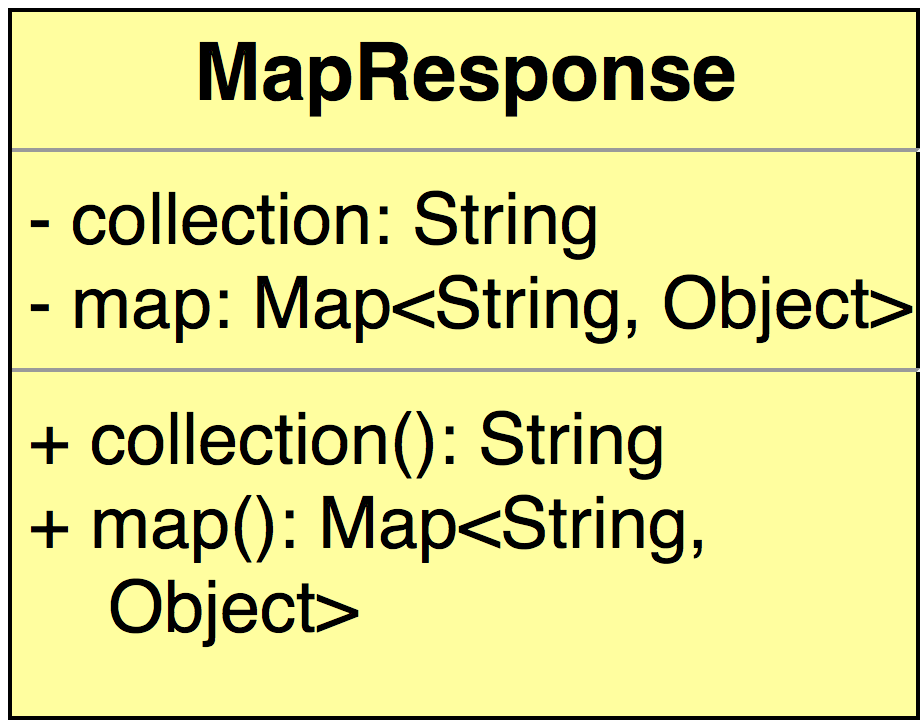
\includegraphics[width=0.3\textwidth,keepaspectratio]{RA/mapResponse.png}
    \caption{Classe MapResponse}
  \end{center}
\end{figure}

\subparagraph{Descrizione}
Classe che rappresenta un messaggio utilizzato per consegnare al
\hyperref[sec:actorbase::actorsystem::actors::clientactor::ClientActor]{ClientActor} una collezione dati, utilizzato per adempiere ad alcune
richieste dell'utente.\\Implementata utilizzando la specifica funzionalità \textit{case class} di Scala,
in modo da poter usufruirne mediante costrutti e algoritmi di
\gloss{pattern matching}.

\subparagraph{Utilizzo}
Questa classe viene utilizzata per mandare una collezione dati all'attore
\hyperref[sec:actorbase::actorsystem::actors::clientactor::ClientActor]{ClientActor}.
Questo viene utilizzato per adempiere ad alcune richieste dell'utente come
la richiesta di restituzione di una collezione.

\subparagraph{Attributi}
\begin{tabular}{| p{2cm} | p{1.5cm} | p{2cm} | p{3cm} | p{8.5cm} |}
  \hline
  Nome & Accesso & Mutabilità & Tipo & Descrizione\\
  \hline
  collection & privato & immutabile & String & Rappresenta il nome di una collezione\\
  \hline
  map & privato & immutabile & Map<String, Object> & Rappresenta una struttura dati contenente le coppie chiave valore da restituire all'utente a seguito di una richiesta\\
  \hline
\end{tabular}

\subparagraph{Metodi}
\begin{tabular}{| p{3cm} | p{1.5cm} | p{3.5cm} | p{9cm} |}
  \hline
  Nome & Accesso & Tipo di ritorno & Descrizione\\
  \hline
  collection & pubblico & String & Metodo che ritorna l'attributo collection\\
  \hline
  map & pubblico & Map<String, Object> & Metodo che ritorna l'attributo map\\
  \hline
\end{tabular}

\paragraph{actorbase::actorsystem::messages::clientactormessages::Response}
\label{sec:actorbase::actorsystem::messages::clientactormessages::Response}

% TODO img
\begin{figure}[H]
  \begin{center}
    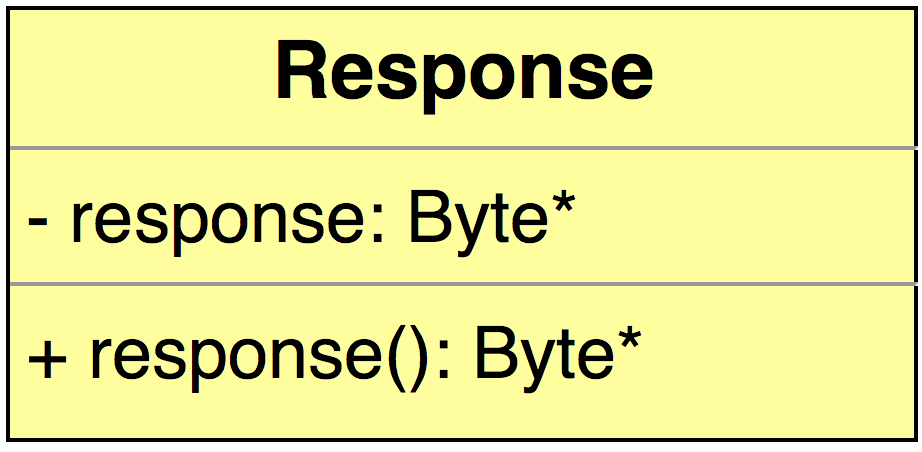
\includegraphics[width=0.3\textwidth,keepaspectratio]{RA/response.png}
    \caption{Classe Response}
  \end{center}
\end{figure}

\subparagraph{Descrizione}
Classe che rappresenta un messaggio utilizzato per consegnare al
\hyperref[sec:actorbase::actorsystem::actors::clientactor::ClientActor]{ClientActor} una stringa, utilizzato per adempiere ad alcune
richieste dell'utente.\\Implementata utilizzando la specifica funzionalità \textit{case class} di Scala,
in modo da poter usufruirne mediante costrutti e algoritmi di
\gloss{pattern matching}.

\subparagraph{Utilizzo}
Questa classe viene utilizzata per mandare una stringa all'attore
\hyperref[sec:actorbase::actorsystem::actors::clientactor::ClientActor]{ClientActor}.
Questo viene utilizzato per adempiere ad alcune richieste dell'utente.

\subparagraph{Attributi}
\begin{tabular}{| p{2cm} | p{1.5cm} | p{2cm} | p{3cm} | p{8.5cm} |}
  \hline
  Nome & Accesso & Mutabilità & Tipo & Descrizione\\
  \hline
  response & privato & immutabile & Array<Byte> & Rappresenta una stringa contenente il messaggio o il valore da restituire all'utente a seguito di una sua richiesta\\
  \hline
\end{tabular}

\subparagraph{Metodi}
\begin{tabular}{| p{3cm} | p{1.5cm} | p{3.5cm} | p{9cm} |}
  \hline
  Nome & Accesso & Tipo di ritorno & Descrizione\\
  \hline
  response & pubblico & Array<Byte> & Metodo che ritorna l'attributo response\\
  \hline
\end{tabular}

%%%%%%%%%%%%%%%%%%%%%%%%%%%%%%%%%%%%%%%%%%%%%%%%%%%%%%%%%%%%%%%%%%%%%%%%%

\subsection{actorbase::actorsystem::messages::mainmessages}
\label{sec:actorbase::actorsystem::messages::mainmessages}

% TODO img
\begin{figure}[H]
  \begin{center}
    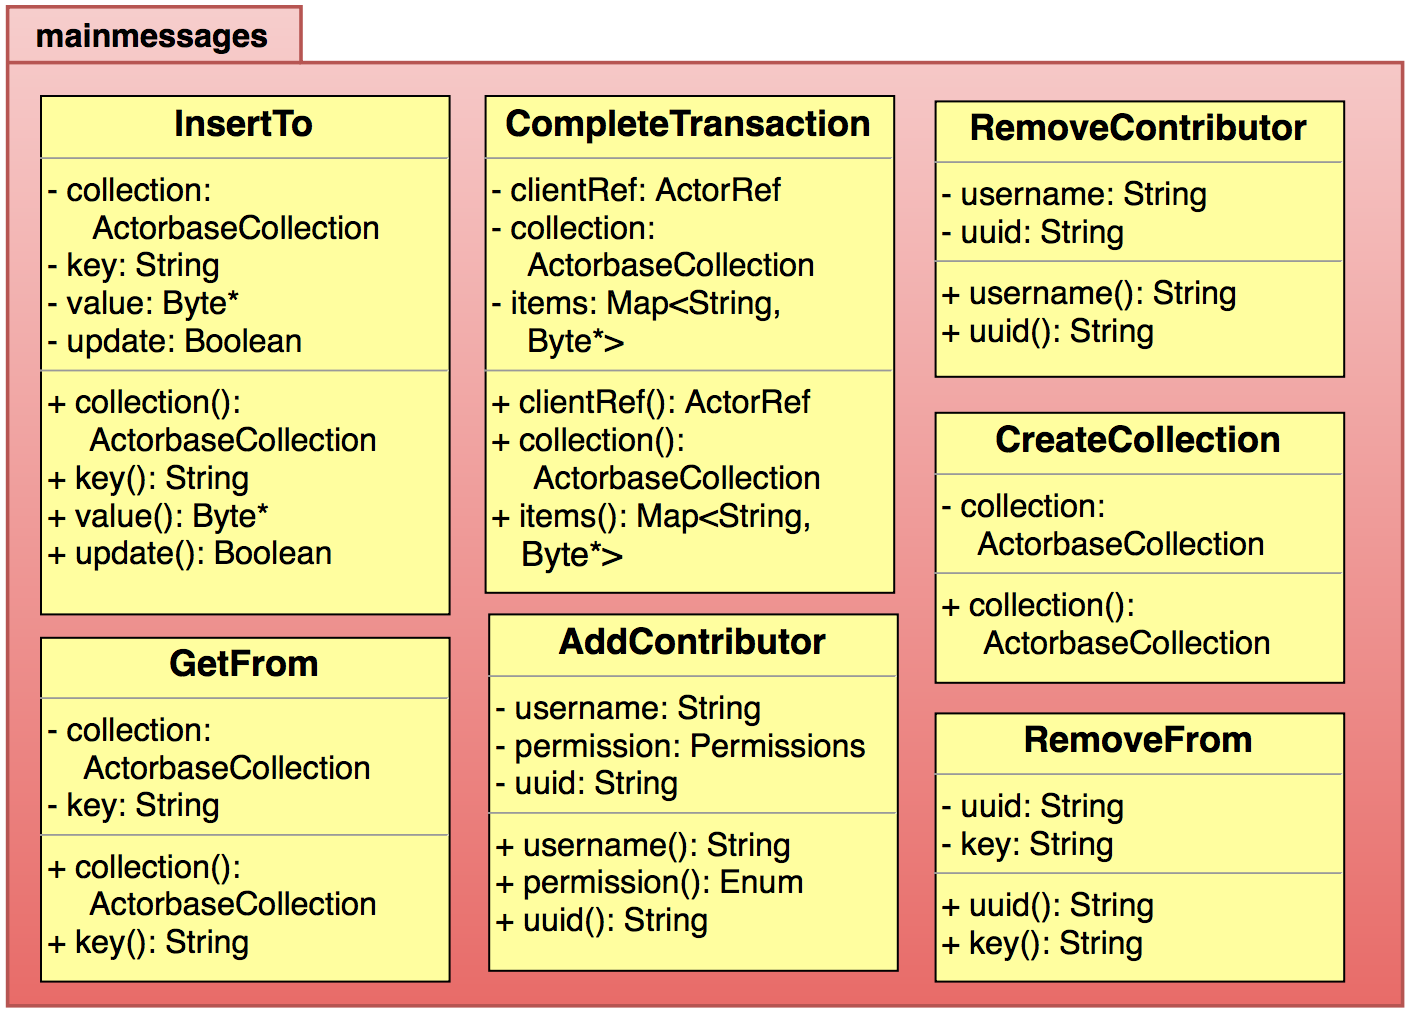
\includegraphics[width=0.9\textwidth,keepaspectratio]{RA/mainmessages.png}
    \caption{Package actorsystem::messages::mainmessages}
  \end{center}
\end{figure}

\subsubsection{Descrizione}
\gloss{Package} contenente i messaggi processabili dall'attore \hyperref[sec:actorbase::actorsystem::actors::main::Main]{Main}.

\subsubsection{Classi}

\paragraph{actorbase::actorsystem::messages::mainmessages::InsertTo}
\label{sec:actorbase::actorsystem::messages::mainmessages::InsertTo}

% TODO img
\begin{figure}[H]
  \begin{center}
    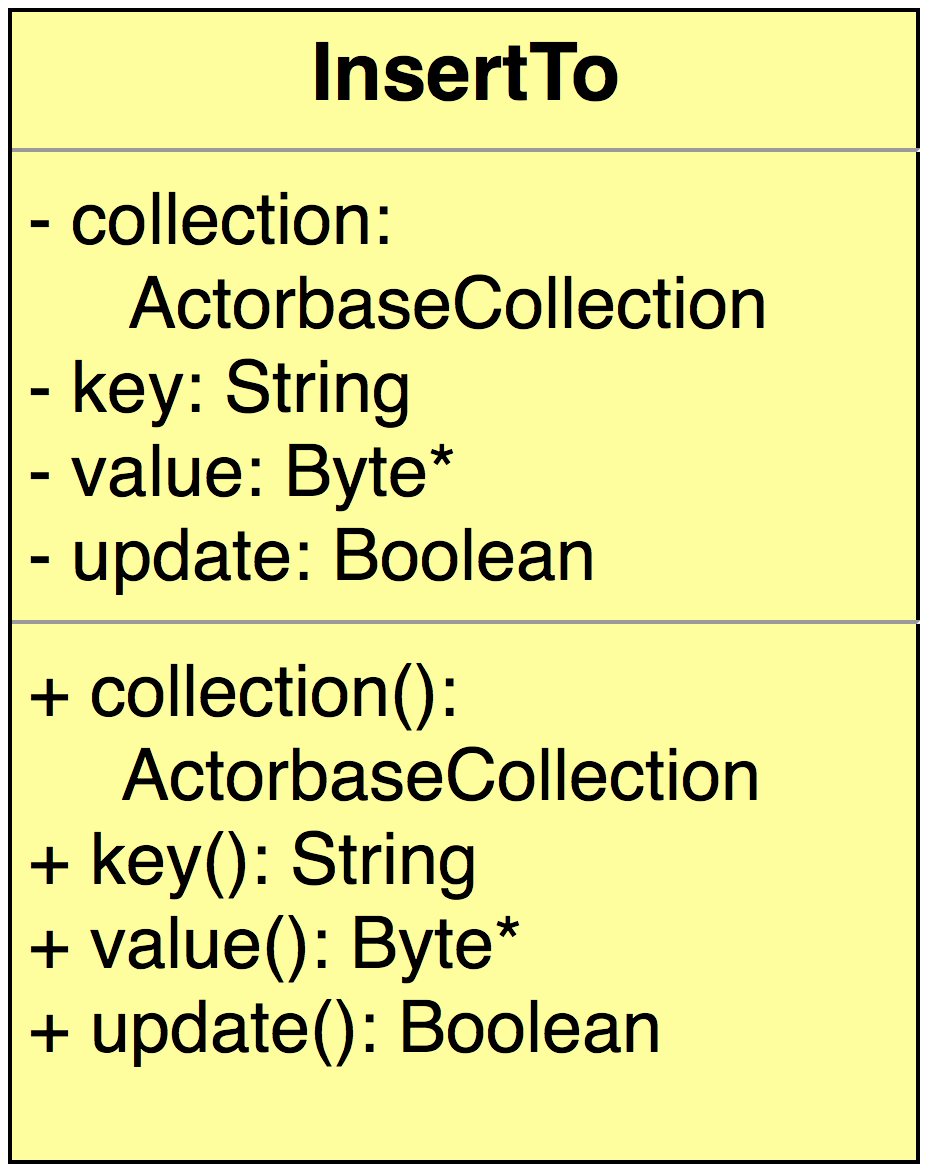
\includegraphics[width=0.3\textwidth,keepaspectratio]{RA/insertTo.png}
    \caption{Classe InsertTo}
  \end{center}
\end{figure}

\subparagraph{Descrizione}
Classe che rappresenta un messaggio utilizzato per richiedere al
\hyperref[sec:actorbase::actorsystem::actors::main::Main]{Main} l'inserimento
di un item.\\Implementata utilizzando la specifica funzionalità
\textit{case class} di Scala,
in modo da poter usufruirne mediante costrutti e algoritmi di
\gloss{pattern matching}.

\subparagraph{Utilizzo}
Questa classe viene utilizzata per mandare una richiesta di inserimento di un
item all'attore
\hyperref[sec:actorbase::actorsystem::actors::main::Main]{Main}.\\Questo attore
provvederà ad inoltrare la richiesta al giusto attore
\hyperref[sec:actorbase::actorsystem::actors::storefinder::Storefinder]{Storefinder}
che rappresenta la \gloss{collezione} in cui inserire l'item. Se non è presente
la collezione in cui inserire l'item questa verrà creata istanziando un nuovo
attore
\hyperref[sec:actorbase::actorsystem::actors::storefinder::Storefinder]{Storefinder},
infine verrà inoltrata la richiesta di inserimento a quest'ultimo.

\subparagraph{Attributi}
\begin{tabular}{| p{2cm} | p{1.5cm} | p{2cm} | p{3cm} | p{8.5cm} |}
  \hline
  Nome & Accesso & Mutabilità & Tipo & Descrizione\\
  \hline
  collection & privato & immutabile & \hyperref[sec:actorbase::actorsystem::utils::ActorbaseCollection]{ActorbaseCollection} & Rappresenta la collezione in cui effettuare l'inserimento \\
  \hline
  key & privato & immutabile & String & Rappresenta la chiave dell'item da inserire\\
  \hline
  value & privato & immutabile & Array<Byte> & Rappresenta il valore dell'item serializzato in array di byte\\
  \hline
  update & privato & immutabile & Boolean & Rappresenta un flag per scegliere se l'inserimento deve poter sovrascrivere un item già presente con la stessa chiave o meno\\
  \hline
\end{tabular}

\subparagraph{Metodi}
\begin{tabular}{| p{3cm} | p{1.5cm} | p{3.5cm} | p{9cm} |}
  \hline
  Nome & Accesso & Tipo di ritorno & Descrizione\\
  \hline
  collection & pubblico & \hyperref[sec:actorbase::actorsystem::utils::ActorbaseCollection]{ActorbaseCollection} & Metodo che ritorna l'attributo collection\\
  \hline
  key & pubblico & String & Metodo che ritorna l'attributo key\\
  \hline
  value & pubblico & Array<Byte> & Metodo che ritorna l'attributo value\\
  \hline
  update & pubblico & Boolean & Metodo che ritorna l'attributo update\\
  \hline
\end{tabular}

\paragraph{actorbase::actorsystem::messages::mainmessages::GetFrom}
\label{sec:actorbase::actorsystem::messages::mainmessages::GetFrom}

% TODO img
\begin{figure}[H]
  \begin{center}
    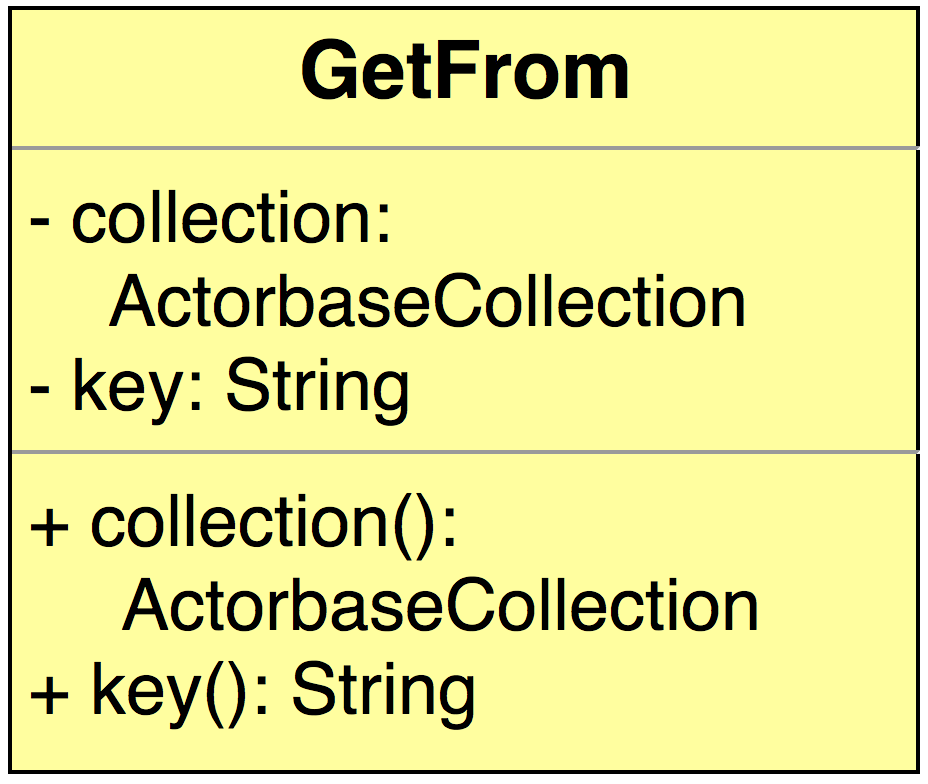
\includegraphics[width=0.3\textwidth,keepaspectratio]{RA/getFrom.png}
    \caption{Classe GetFrom}
  \end{center}
\end{figure}

\subparagraph{Descrizione}
Classe che rappresenta un messaggio utilizzato per richiedere al
\hyperref[sec:actorbase::actorsystem::actors::main::Main]{Main} di ritornare items o collezioni.\\Implementata utilizzando la specifica funzionalità \textit{case class} di Scala,
in modo da poter usufruirne mediante costrutti e algoritmi di
\gloss{pattern matching}.

\subparagraph{Utilizzo}
Questa classe viene utilizzata per mandare una richiesta di ritorno di un item o di una collezione all'attore
\hyperref[sec:actorbase::actorsystem::actors::main::Main]{Main}.\\Questo attore
provvederà ad inoltrare la richiesta al giusto attore \hyperref[sec:actorbase::actorsystem::actors::storefinder::Storefinder]{Storefinder}.\\Il
parametro in ingresso \textit{key} determina se l'utente richiede un singolo
item o una intera collezione.

\subparagraph{Attributi}
\begin{tabular}{| p{2cm} | p{1.5cm} | p{2cm} | p{3cm} | p{8.5cm} |}
  \hline
  Nome & Accesso & Mutabilità & Tipo & Descrizione\\
  \hline
  collection & privato & immutabile & \hyperref[sec:actorbase::actorsystem::utils::ActorbaseCollection]{ActorbaseCollection} & Rappresenta la collezione in cui cercare o la collezione da ritornare \\
  \hline
  key & privato & immutabile & String & Rappresenta la chiave dell'item da cercare\\
  \hline
\end{tabular}

\subparagraph{Metodi}
\begin{tabular}{| p{3cm} | p{1.5cm} | p{3.5cm} | p{9cm} |}
  \hline
  Nome & Accesso & Tipo di ritorno & Descrizione\\
  \hline
  collection & pubblico & \hyperref[sec:actorbase::actorsystem::utils::ActorbaseCollection]{ActorbaseCollection} & Metodo che ritorna l'attributo collection\\
  \hline
  key & pubblico & String & Metodo che ritorna l'attributo key\\
  \hline
\end{tabular}

% TODO COMPLETE TRANSACTION NON È DESCRITTO GIUSTO CREDO
\paragraph{actorbase::actorsystem::messages::mainmessages::CompleteTransaction}
\label{sec:actorbase::actorsystem::messages::mainmessages::CompleteTransaction}

% TODO img
\begin{figure}[H]
  \begin{center}
    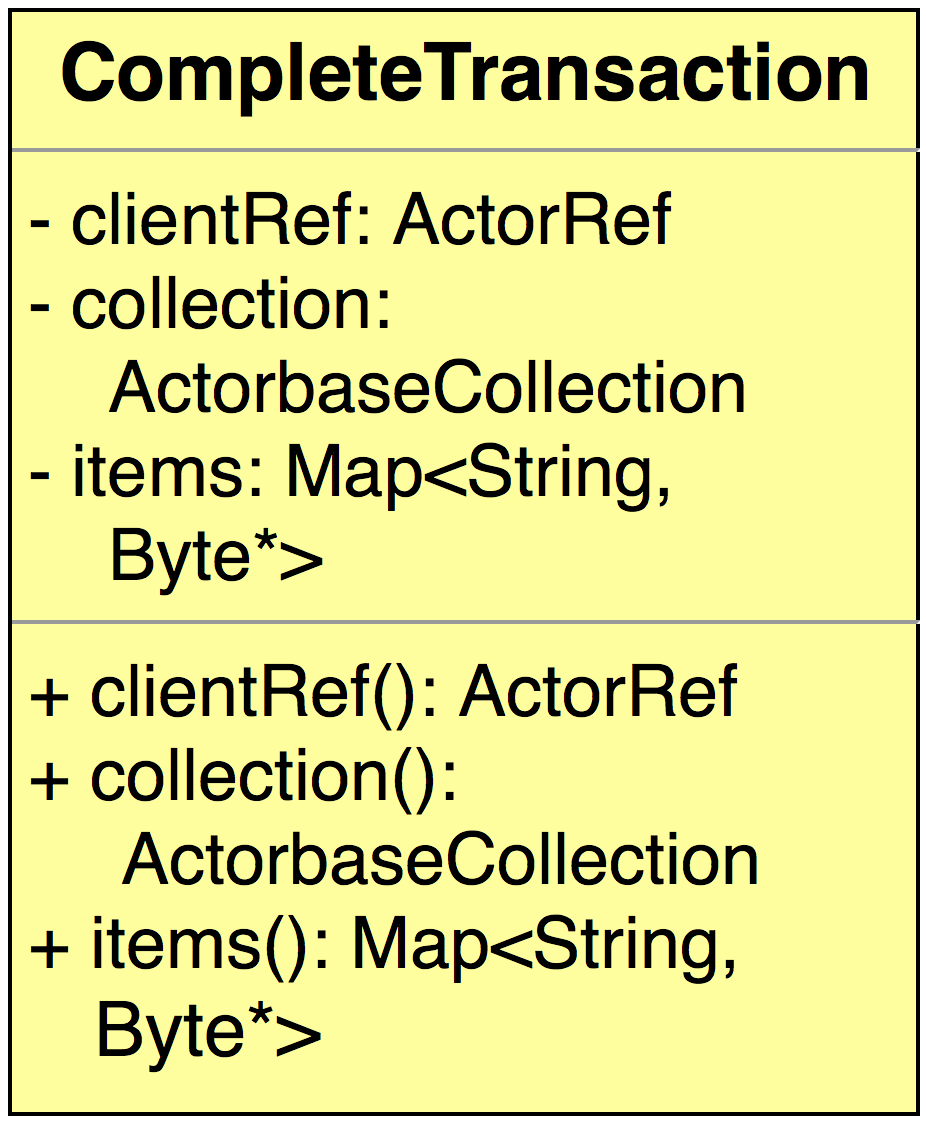
\includegraphics[width=0.3\textwidth,keepaspectratio]{RA/completeTransaction.png}
    \caption{Classe CompleteTransaction}
  \end{center}
\end{figure}

\subparagraph{Descrizione}
Classe che rappresenta un messaggio utilizzato per assemblare parti di
\gloss{collezioni} provenienti dagli \gloss{attori} di tipo
\hyperref[sec:actorbase::actorsystem::actors::storekeeper::Storekeeper]{Storekeeper}
verso l'\gloss{attore}
\hyperref[sec:actorbase::actorsystem::actors::main::Main]{Main}.\\Implementata
utilizzando la specifica funzionalità \textit{case class} di Scala, in modo da
poter usufruirne mediante costrutti e algoritmi di \gloss{pattern matching}.

\subparagraph{Utilizzo}
Questa classe viene utilizzata per assemblare le parti di \gloss{collezione} provenienti dagli \gloss{attori}
di tipo \hyperref[sec:actorbase::actorsystem::actors::storekeeper::Storekeeper]{Storekeeper} verso l'\gloss{attore}
\hyperref[sec:actorbase::actorsystem::actors::main::Main]{Main}.\\Quest'ultimo
dovrà attendere tutti i messaggi
\hyperref[sec:actorbase::actorsystem::messages::mainmessages::CompleteTransaction]{CompleteTransaction}
necessari per costruire un intera \gloss{collezione} da restituire all'utente.\\Questo
messaggio è utilizzato quando un utente richiede un intera \gloss{collezione}.

\subparagraph{Attributi}
\begin{tabular}{| p{2cm} | p{1.5cm} | p{2cm} | p{3cm} | p{8.5cm} |}
  \hline
  Nome & Accesso & Mutabilità & Tipo & Descrizione\\
  \hline
  clientRef & privato & immutabile & ActorRef & Rappresenta il riferimento all'attore \hyperref[sec:actorbase::actorsystem::actors::clientactor::ClientActor]{ClientActor} che ha effettuato la richiesta di ritorno collezione\\
  \hline
  collection & privato & immutabile & \hyperref[sec:actorbase::actorsystem::utils::ActorbaseCollection]{ActorbaseCollection} & Rappresenta la collezione di cui fanno parte gli item passati in questo messaggio\\
  \hline
  items & privato & immutabile & Map<String, Array<Byte> > & Rappresenta una mappa di items, in particolare rappresentano un pezzo della collezione richiesta\\
  \hline
\end{tabular}

\subparagraph{Metodi}
\begin{tabular}{| p{3cm} | p{1.5cm} | p{3.5cm} | p{9cm} |}
  \hline
  Nome & Accesso & Tipo di ritorno & Descrizione\\
  \hline
  clientRef & pubblico & ActorRef & Metodo che ritorna l'attributo clientRef\\
  \hline
  collection & pubblico & \hyperref[sec:actorbase::actorsystem::utils::ActorbaseCollection]{ActorbaseCollection} & Metodo che ritorna l'attributo collection\\
  \hline
  items & pubblico & Map<String, Array<Byte> > & Metodo che ritorna l'attributo key\\
  \hline
\end{tabular}

\paragraph{actorbase::actorsystem::messages::mainmessages::RemoveFrom}
\label{sec:actorbase::actorsystem::messages::mainmessages::RemoveFrom}

% TODO img
\begin{figure}[H]
  \begin{center}
    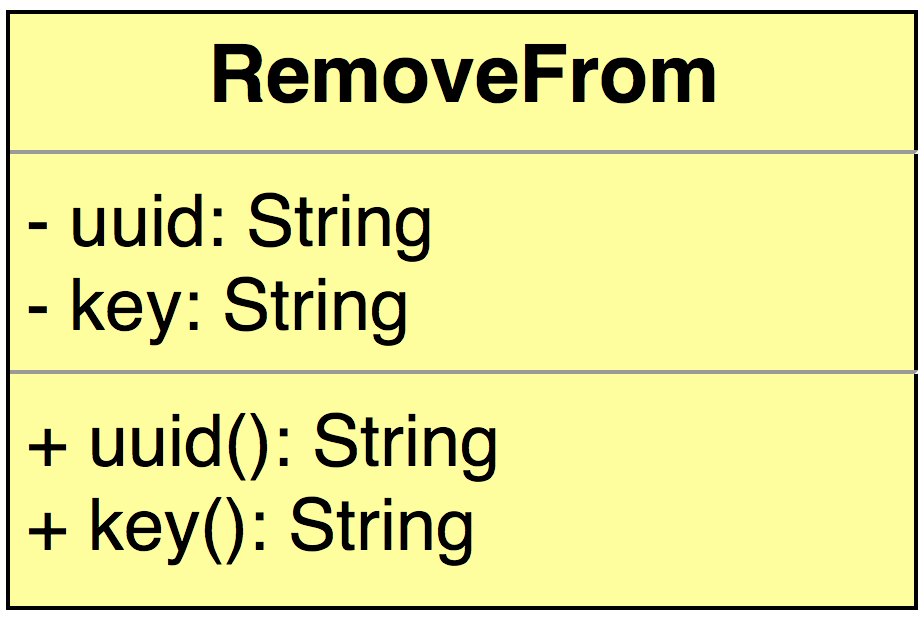
\includegraphics[width=0.3\textwidth,keepaspectratio]{RA/removeFrom.png}
    \caption{Classe RemoveFrom}
  \end{center}
\end{figure}

\subparagraph{Descrizione}
Classe che rappresenta un messaggio utilizzato per richiedere la rimozione di
item all'attore \hyperref[sec:actorbase::actorsystem::actors::main::Main]{Main}.\\Implementata utilizzando la specifica funzionalità \textit{case class} di Scala, in modo da poter usufruirne mediante costrutti e algoritmi di
\gloss{pattern matching}.

\subparagraph{Utilizzo}
Questa classe viene utilizzata per rimuovere items dal sistema. L'attore
\hyperref[sec:actorbase::actorsystem::actors::main::Main]{Main} dovrà
inoltrare la richiesta al giusto attore \hyperref[sec:actorbase::actorsystem::actors::storefinder::Storefinder]{Storefinder}, ovvero colui che rappresenta la collezione in cui effettuare l'operazione.

\subparagraph{Attributi}
\begin{tabular}{| p{2cm} | p{1.5cm} | p{2cm} | p{3cm} | p{8.5cm} |}
  \hline
  Nome & Accesso & Mutabilità & Tipo & Descrizione\\
  \hline
  uuid & privato & immutabile & String & Rappresenta l'id della collezione da cui eliminare l'\gloss{item}\\
  \hline
  key & privato & immutabile & String & Rappresenta la chiave dell'item da eliminare\\
  \hline
\end{tabular}

\subparagraph{Metodi}
\begin{tabular}{| p{3cm} | p{1.5cm} | p{3.5cm} | p{9cm} |}
  \hline
  Nome & Accesso & Tipo di ritorno & Descrizione\\
  \hline
  uuid & pubblico & String & Metodo che ritorna l'attributo uuid\\
  \hline
  key & pubblico & String & Metodo che ritorna l'attributo key\\
  \hline
\end{tabular}

\paragraph{actorbase::actorsystem::messages::mainmessages::AddContributor}
\label{sec:actorbase::actorsystem::messages::mainmessages::AddContributor}

% TODO img
\begin{figure}[H]
  \begin{center}
    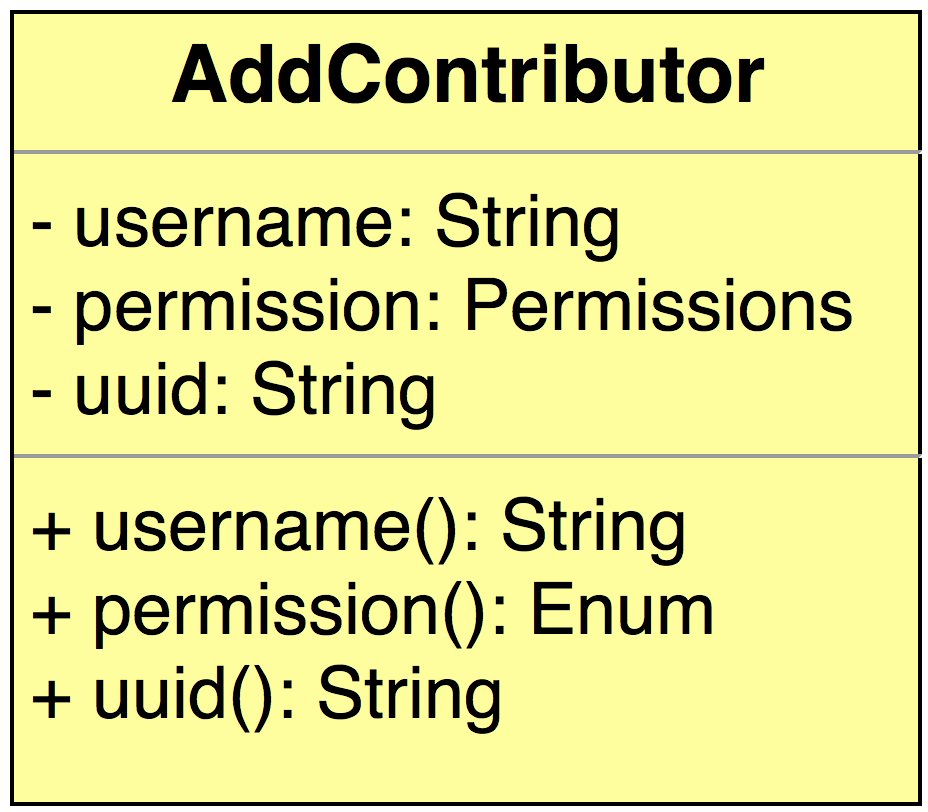
\includegraphics[width=0.3\textwidth,keepaspectratio]{RA/addContributor.png}
    \caption{Classe AddContributor}
  \end{center}
\end{figure}

\subparagraph{Descrizione}
Classe che rappresenta un messaggio utilizzato per richiedere l'aggiunta di un
collaboratore ad una \gloss{collezione} all'attore \hyperref[sec:actorbase::actorsystem::actors::main::Main]{Main}.\\Implementata
utilizzando la specifica funzionalità \textit{case class} di Scala, in modo da poter usufruirne mediante costrutti e algoritmi di
\gloss{pattern matching}.

\subparagraph{Utilizzo}
Questa classe viene utilizzata per richiedere l'aggiunta di collaboratori ad
una collezione. L'attore
\hyperref[sec:actorbase::actorsystem::actors::main::Main]{Main} dovrà aggiungere
lo username del collaboratore designato alla collezione richiesta.

\subparagraph{Attributi}
\begin{tabular}{| p{2cm} | p{1.5cm} | p{2cm} | p{3cm} | p{8.5cm} |}
  \hline
  Nome & Accesso & Mutabilità & Tipo & Descrizione\\
  \hline
  username & privato & immutabile & String & Rappresenta lo \gloss{username} del \gloss{collaboratore} da aggiungere alla \gloss{collezione}\\
  \hline
  permission & privato & immutabile & Enum & Rappresenta il tipo di permessi da assegnare al \gloss{collaboratore}\\
  \hline
  uuid & privato & immutabile & String & Rappresenta l'id della \gloss{collezione} a cui aggiungere il \gloss{collaboratore}\\
  \hline
\end{tabular}

\subparagraph{Metodi}
\begin{tabular}{| p{3cm} | p{1.5cm} | p{3.5cm} | p{9cm} |}
  \hline
  Nome & Accesso & Tipo di ritorno & Descrizione\\
  \hline
  username & pubblico & String & Metodo che ritorna l'attributo username\\
  \hline
  permission & pubblico & Enum & Metodo che ritorna l'attributo permission\\
  \hline
  uuid & pubblico & String & Metodo che ritorna l'attributo uuid\\
  \hline
\end{tabular}

\paragraph{actorbase::actorsystem::messages::mainmessages::RemoveContributor}
\label{sec:actorbase::actorsystem::messages::mainmessages::RemoveContributor}

% TODO img
\begin{figure}[H]
  \begin{center}
    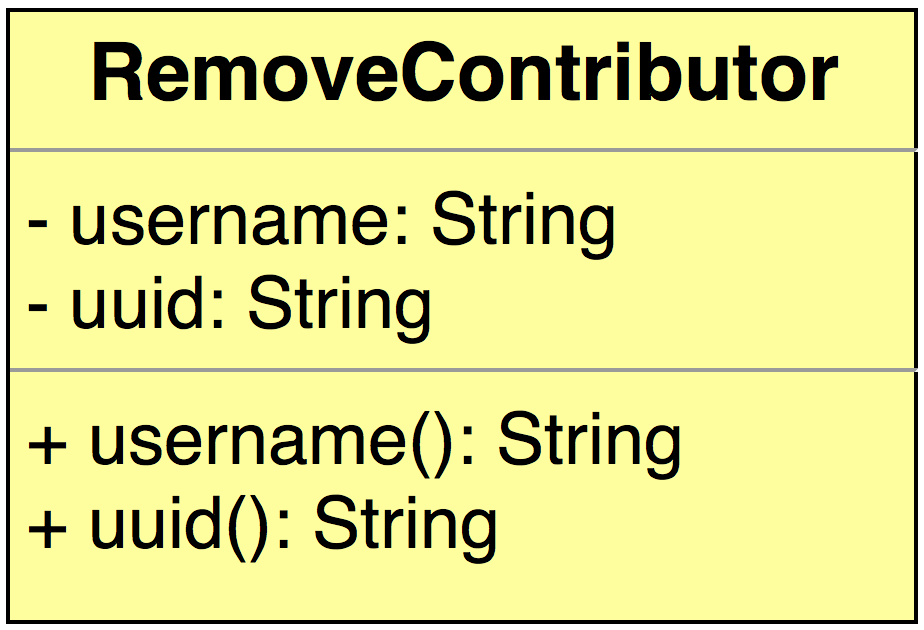
\includegraphics[width=0.3\textwidth,keepaspectratio]{RA/removeContributor.png}
    \caption{Classe RemoveContributor}
  \end{center}
\end{figure}

\subparagraph{Descrizione}
Classe che rappresenta un messaggio utilizzato per richiedere la rimozione di un
collaboratore ad una collezione all'attore \hyperref[sec:actorbase::actorsystem::actors::main::Main]{Main}.\\Implementata
utilizzando la specifica funzionalità \textit{case class} di Scala, in modo da poter usufruirne mediante costrutti e algoritmi di
\gloss{pattern matching}.

\subparagraph{Utilizzo}
Questa classe viene utilizzata per richiedere la rimozione di collaboratori ad
una collezione. L'attore
\hyperref[sec:actorbase::actorsystem::actors::main::Main]{Main} dovrà rimuovere
lo username del collaboratore designato alla collezione richiesta.

\subparagraph{Attributi}
\begin{tabular}{| p{2cm} | p{1.5cm} | p{2cm} | p{3cm} | p{8.5cm} |}
  \hline
  Nome & Accesso & Mutabilità & Tipo & Descrizione\\
  \hline
  username & privato & immutabile & String & Rappresenta lo username del collaboratore da rimuovere dalla collezione\\
  \hline
  uuid & privato & immutabile & String & Rappresenta l'id della collezione da cui rimuovere il collaboratore\\
  \hline
\end{tabular}

\subparagraph{Metodi}
\begin{tabular}{| p{3cm} | p{1.5cm} | p{3.5cm} | p{9cm} |}
  \hline
  Nome & Accesso & Tipo di ritorno & Descrizione\\
  \hline
  username & pubblico & String & Metodo che ritorna l'attributo username\\
  \hline
  uuid & pubblico & String & Metodo che ritorna l'attributo uuid\\
  \hline
\end{tabular}

\paragraph{actorbase::actorsystem::messages::mainmessages::CreateCollection}
\label{sec:actorbase::actorsystem::messages::mainmessages::CreateCollection}

% TODO img
\begin{figure}[H]
  \begin{center}
    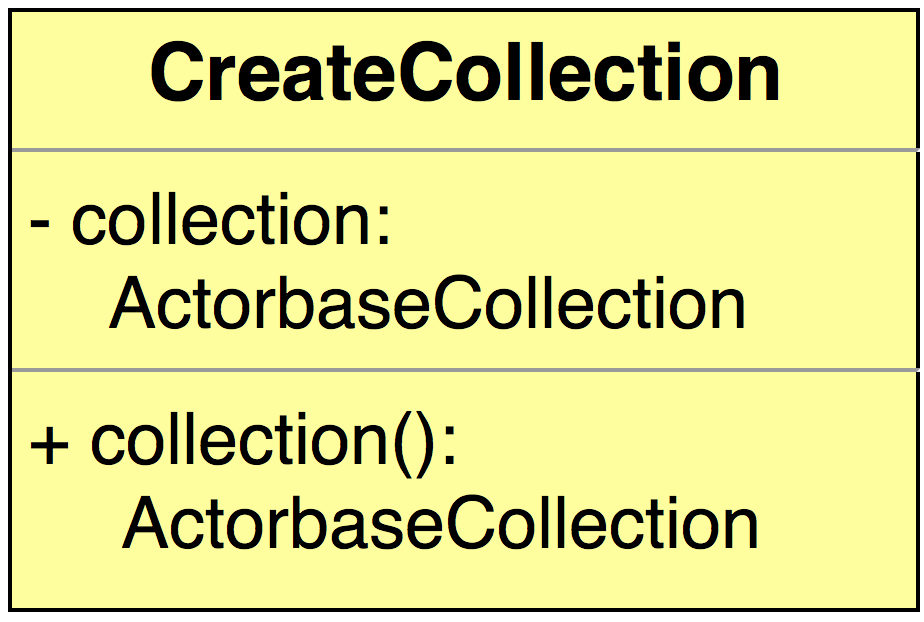
\includegraphics[width=0.3\textwidth,keepaspectratio]{RA/createCollection.png}
    \caption{Classe CreateCollection}
  \end{center}
\end{figure}

\subparagraph{Descrizione}
Classe che rappresenta un messaggio utilizzato per richiedere la creazione di una collezione all'attore \hyperref[sec:actorbase::actorsystem::actors::main::Main]{Main}.\\Implementata
utilizzando la specifica funzionalità \textit{case class} di Scala, in modo da poter usufruirne mediante costrutti e algoritmi di
\gloss{pattern matching}.

\subparagraph{Utilizzo}
Questa classe viene utilizzata per richiedere la creazione di una collezione.\\L'attore
\hyperref[sec:actorbase::actorsystem::actors::main::Main]{Main} provvederà a creare la nuova collezione e a creare un attore \hyperref[sec:actorbase::actorsystem::actors::storefinder::Storefinder]{Storefinder}
adibito alla gestione di quest'ultima.

\subparagraph{Attributi}
\begin{tabular}{| p{2cm} | p{1.5cm} | p{2cm} | p{3cm} | p{8.5cm} |}
  \hline
  Nome & Accesso & Mutabilità & Tipo & Descrizione\\
  \hline
  collection & privato & immutabile & \hyperref[sec:actorbase::actorsystem::utils::ActorbaseCollection]{ActorbaseCollection} & Collezione da aggiungere al sistema\\
  \hline
\end{tabular}

\subparagraph{Metodi}
\begin{tabular}{| p{3cm} | p{1.5cm} | p{3.5cm} | p{9cm} |}
  \hline
  Nome & Accesso & Tipo di ritorno & Descrizione\\
  \hline
  collection & pubblico & \hyperref[sec:actorbase::actorsystem::utils::ActorbaseCollection]{ActorbaseCollection} & Metodo che ritorna l'attributo collection\\
  \hline
\end{tabular}

%%%%%%%%%%%%%%%%%%%%%%%%%%%%%%%%%%%%%%%%%%%%%%%%%%%%%%%%%%%%%%%%%%%%%%%%%

\subsection{actorbase::actorsystem::messages::storefindermessages}
\label{sec:actorbase::actorsystem::messages::storefindermessages}

% TODO img
\begin{figure}[H]
  \begin{center}
    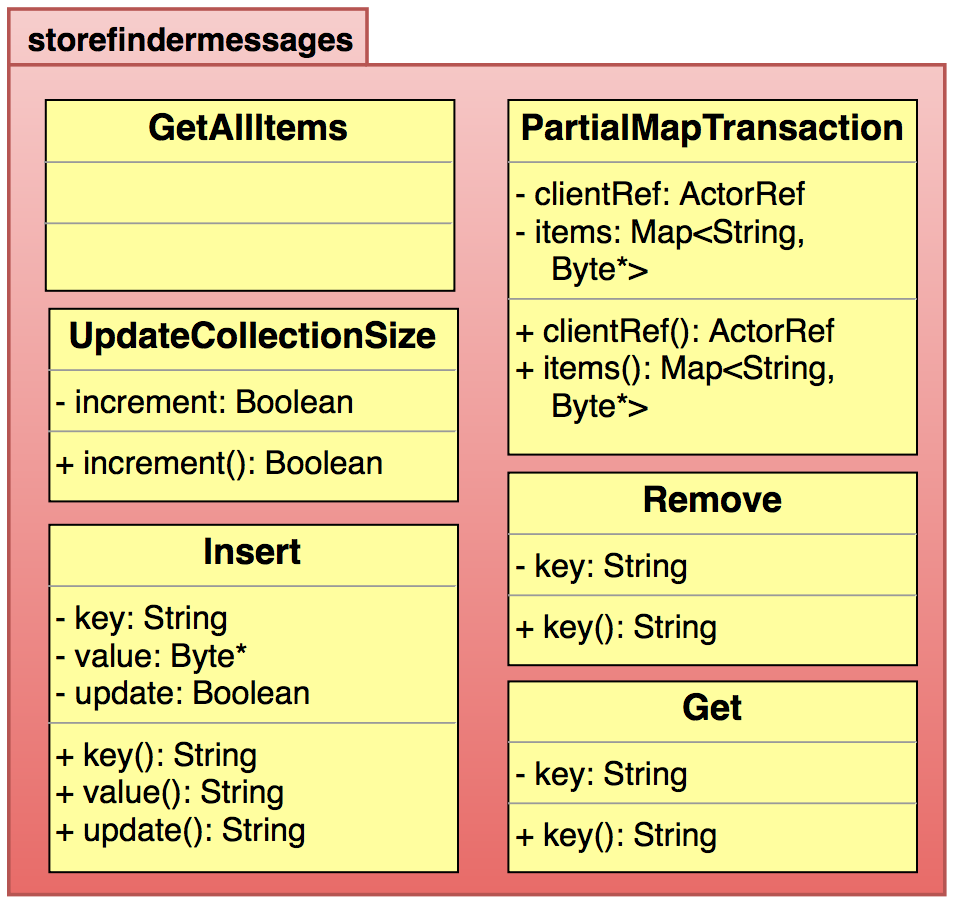
\includegraphics[width=0.7\textwidth,keepaspectratio]{RA/storefindermessages.png}
    \caption{Package actorsystem::messages::storefindermessages}
  \end{center}
\end{figure}

\subsubsection{Descrizione}
\gloss{Package} contenente i messaggi processabili dall'attore \hyperref[sec:actorbase::actorsystem::actors::storefinder::Storefinder]{Storefinder}.

\subsubsection{Classi}

\paragraph{actorbase::actorsystem::messages::storefinder::GetAllItems}
\label{sec:actorbase::actorsystem::messages::storefinder::GetAllItems}

% TODO img
\begin{figure}[H]
  \begin{center}
    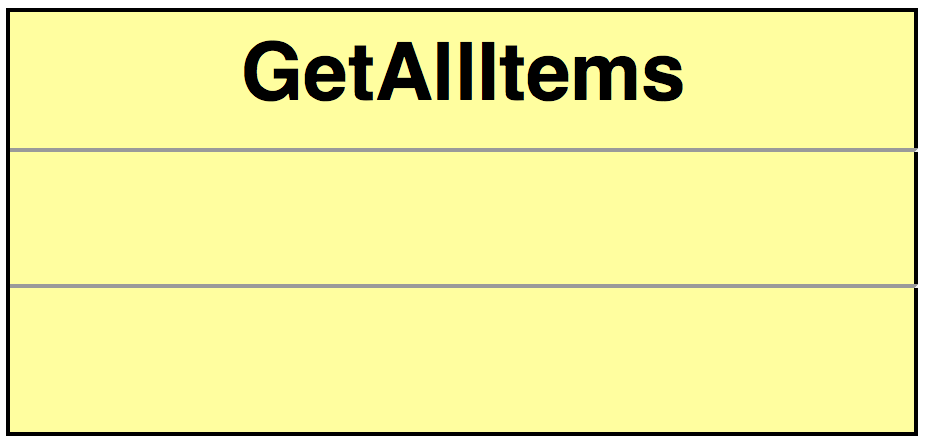
\includegraphics[width=0.3\textwidth,keepaspectratio]{RA/getAllItems.png}
    \caption{Classe Storefinder}
  \end{center}
\end{figure}

\subparagraph{Descrizione}
Classe che rappresenta un messaggio utilizzato per richiedere allo
\hyperref[sec:actorbase::actorsystem::actors::storefinder::Storefinder]{Storefinder} di ritornare tutti gli item mappati dai propri \hyperref[sec:actorbase::actorsystem::actors::storekeeper::Storekeeper]{Storekeeper}.\\Implementata utilizzando la specifica funzionalità \textit{case class} di Scala,
in modo da poter usufruirne mediante costrutti e algoritmi di
\gloss{pattern matching}.

\subparagraph{Utilizzo}
Questa classe viene utilizzata per richiedere tutti gli items mappati dallo
\hyperref[sec:actorbase::actorsystem::actors::storefinder::Storefinder]{Storefinder}.\\Questo attore provvederà a mandare richieste Get agli attori
\hyperref[sec:actorbase::actorsystem::actors::storekeeper::Storekeeper]{Storekeeper}.\\Questo tipo di messaggio è ricevuto quando un utente intende
richiedere intere collezioni.

\paragraph{actorbase::actorsystem::messages::storefinder::UpdateCollectionSize}
\label{sec:actorbase::actorsystem::messages::storefinder::UpdateCollectionSize}

% TODO img
\begin{figure}[H]
  \begin{center}
    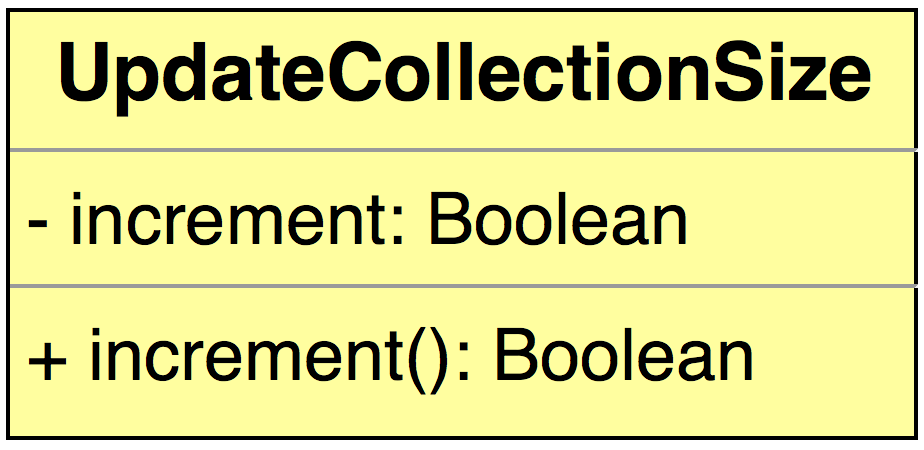
\includegraphics[width=0.3\textwidth,keepaspectratio]{RA/updateCollectionSize.png}
    \caption{Classe UpdateCollectionSize}
  \end{center}
\end{figure}

\subparagraph{Descrizione}
Classe che rappresenta un messaggio utilizzato per aggiornare il numero di item
contenuti in una collezione.\\Implementata utilizzando la specifica funzionalità \textit{case class} di Scala,
in modo da poter usufruirne mediante costrutti e algoritmi di
\gloss{pattern matching}.

\subparagraph{Utilizzo}
Questa classe viene utilizzata per tenere aggiornate le dimensioni delle
collezioni quando si inseriscono o rimuovono items da esse.

\subparagraph{Attributi}
\begin{tabular}{| p{2cm} | p{1.5cm} | p{2cm} | p{3cm} | p{8.5cm} |}
  \hline
  Nome & Accesso & Mutabilità & Tipo & Descrizione\\
  \hline
  increment & privato & immutabile & Boolean & flag che indica se c'è stato un incremento o un decremento nella collezione (true se incremento)\\
  \hline
\end{tabular}

\subparagraph{Metodi}
\begin{tabular}{| p{3cm} | p{1.5cm} | p{3.5cm} | p{9cm} |}
  \hline
  Nome & Accesso & Tipo di ritorno & Descrizione\\
  \hline
  increment & pubblico & Boolean & Metodo che ritorna l'attributo increment\\
  \hline
\end{tabular}

\paragraph{actorbase::actorsystem::messages::storefinder::Get}
\label{sec:actorbase::actorsystem::messages::storefinder::Get}

% TODO img
\begin{figure}[H]
  \begin{center}
    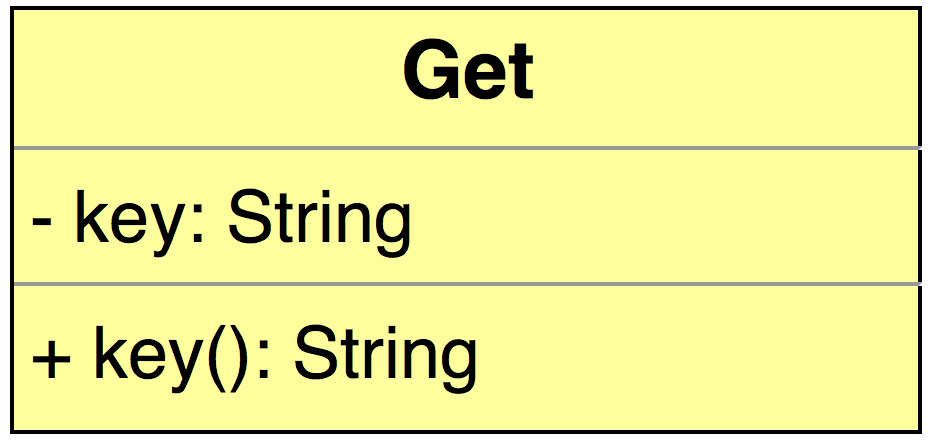
\includegraphics[width=0.3\textwidth,keepaspectratio]{RA/getSF.png}
    \caption{Classe Get}
  \end{center}
\end{figure}

\subparagraph{Descrizione}
Classe che rappresenta un messaggio utilizzato per richiedere un item.\\Implementata utilizzando la specifica funzionalità \textit{case class} di Scala,
in modo da poter usufruirne mediante costrutti e algoritmi di
\gloss{pattern matching}.

\subparagraph{Utilizzo}
Questa classe viene utilizzata per richiedere un item da restituire
all'utente.\\Quando riceve questo messaggio l'attore provvederà a inoltrare la
richiesta allo \hyperref[sec:actorbase::actorsystem::actors::storekeeper::Storekeeper]{Storekeeper} esatto, ovvero colui che contiene l'item mappato dalla chiave inserita.

\subparagraph{Attributi}
\begin{tabular}{| p{2cm} | p{1.5cm} | p{2cm} | p{3cm} | p{8.5cm} |}
  \hline
  Nome & Accesso & Mutabilità & Tipo & Descrizione\\
  \hline
  key & privato & immutabile & String & Rappresenta la chiave dell'item da restituire\\
  \hline
\end{tabular}

\subparagraph{Metodi}
\begin{tabular}{| p{3cm} | p{1.5cm} | p{3.5cm} | p{9cm} |}
  \hline
  Nome & Accesso & Tipo di ritorno & Descrizione\\
  \hline
  key & pubblico & String & Metodo che ritorna l'attributo key\\
  \hline
\end{tabular}

\paragraph{actorbase::actorsystem::messages::storefinder::PartialMapTransaction}
\label{sec:actorbase::actorsystem::messages::storefinder::PartialMapTransaction}

% TODO img
\begin{figure}[H]
  \begin{center}
    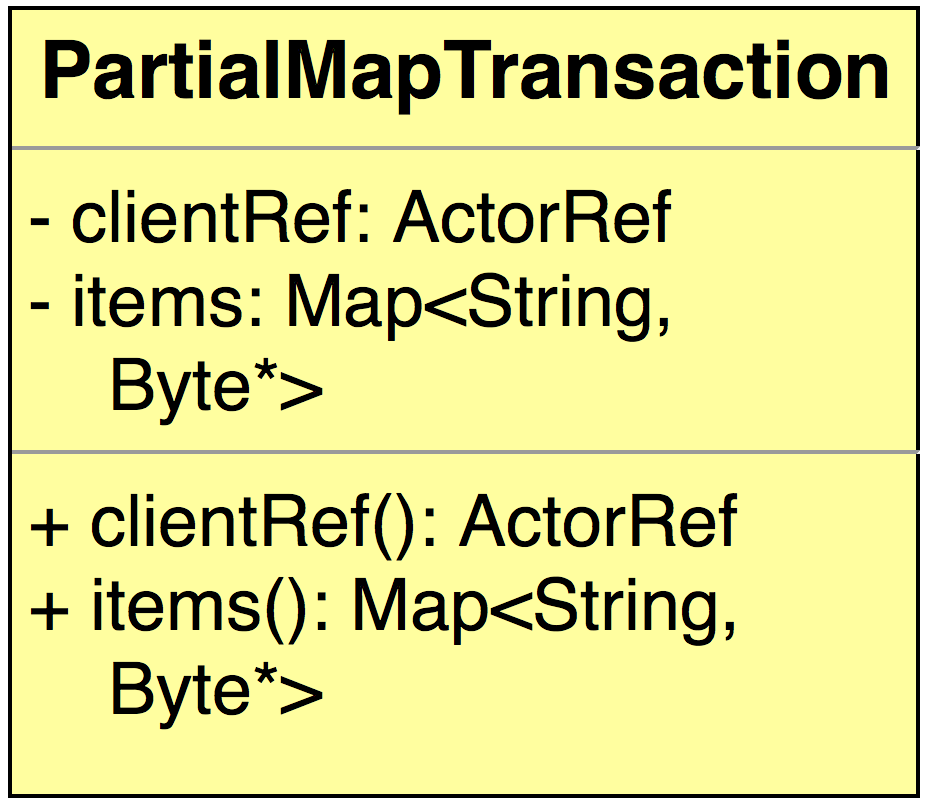
\includegraphics[width=0.3\textwidth,keepaspectratio]{RA/partialMapTransaction.png}
    \caption{Classe PartialMapTransaction}
  \end{center}
\end{figure}

\subparagraph{Descrizione}
Classe che rappresenta un messaggio utilizzato per ricevere parti di \gloss{collezione}
da inviare all'attore \gloss{parent}.\\Implementata utilizzando la specifica
funzionalità \textit{case class} di Scala, in modo da poter usufruirne mediante
costrutti e algoritmi di \gloss{pattern matching}.

\subparagraph{Utilizzo}
Questa classe viene utilizzata per ricevere parti di \gloss{collezione} a
seguito di una richiesta di un' intera \gloss{collezione} da parte di un
utente.\\Quando riceve questo messaggio l'\gloss{attore} provvederà a inoltrare
la mappa di \gloss{item} all'\gloss{attore}
\hyperref[sec:actorbase::actorsystem::actors::main::Main]{Main}, il quale
provvederà ad assemblare tutta la \gloss{collezione} da restituire all'utente.

\subparagraph{Attributi}
\begin{tabular}{| p{2cm} | p{1.5cm} | p{2cm} | p{3cm} | p{8.5cm} |}
  \hline
  Nome & Accesso & Mutabilità & Tipo & Descrizione\\
  \hline
  clientRef & privato & immutabile & ActorRef & Rappresenta il riferimento all'attore \hyperref[sec:actorbase::actorsystem::actors::clientactor::ClientActor]{ClientActor} che ha richiesto la collezione\\
  \hline
  items & privato & immutabile & Map<String, Array<Byte> > & Rappresenta una mappa contenente le coppie chiave valore degli \gloss{item} della \gloss{collezione} da restituire\\
  \hline
\end{tabular}

\subparagraph{Metodi}
\begin{tabular}{| p{3cm} | p{1.5cm} | p{3.5cm} | p{9cm} |}
  \hline
  Nome & Accesso & Tipo di ritorno & Descrizione\\
  \hline
  clientRef & pubblico & ActorRef & Metodo che ritorna l'attributo clientRef\\
  \hline
  items & pubblico & Map<String, Array<Byte> > & Metodo che ritorna l'attributo items\\
  \hline
\end{tabular}

\paragraph{actorbase::actorsystem::messages::storefinder::Remove}
\label{sec:actorbase::actorsystem::messages::storefinder::Remove}

% TODO img
\begin{figure}[H]
  \begin{center}
    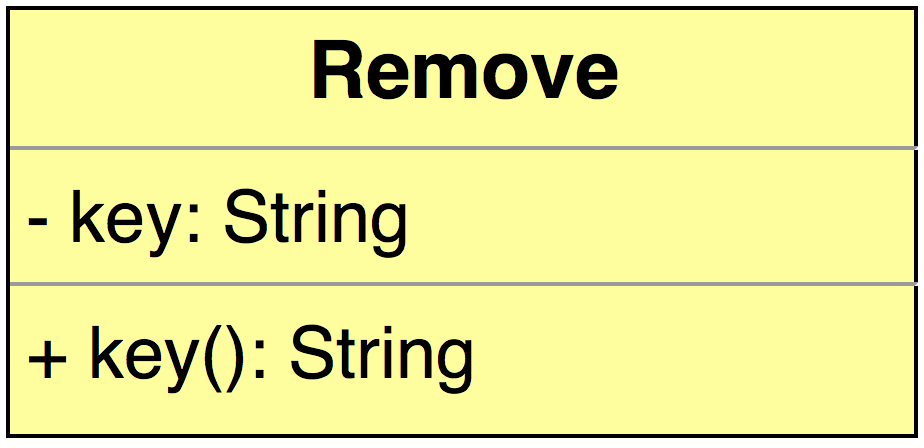
\includegraphics[width=0.3\textwidth,keepaspectratio]{RA/remove.png}
    \caption{Classe Remove}
  \end{center}
\end{figure}

\subparagraph{Descrizione}
Classe che rappresenta un messaggio utilizzato per richiedere la rimozione di un
\gloss{item}.\\Implementata utilizzando la specifica funzionalità \textit{case
  class} di Scala, in modo da poter usufruirne mediante costrutti e algoritmi di
\gloss{pattern matching}.

\subparagraph{Utilizzo}
Questa classe viene utilizzata per richiedere la rimozione di un \gloss{item} dal
sistema.\\Quando riceve questo messaggio l'attore provvederà a inoltrare la
richiesta allo \hyperref[sec:actorbase::actorsystem::actors::storekeeper::Storekeeper]{Storekeeper}
giusto.

\subparagraph{Attributi}
\begin{tabular}{| p{2cm} | p{1.5cm} | p{2cm} | p{3cm} | p{8.5cm} |}
  \hline
  Nome & Accesso & Mutabilità & Tipo & Descrizione\\
  \hline
  key & privato & immutabile & String & Rappresenta la chiave dell'elemento da rimuovere dalla collezione rappresentata da questo attore\\
  \hline
\end{tabular}

\subparagraph{Metodi}
\begin{tabular}{| p{3cm} | p{1.5cm} | p{3.5cm} | p{9cm} |}
  \hline
  Nome & Accesso & Tipo di ritorno & Descrizione\\
  \hline
  key & pubblico & String & Metodo che ritorna l'attributo key\\
  \hline
\end{tabular}

\paragraph{actorbase::actorsystem::messages::storefinder::Insert}
\label{sec:actorbase::actorsystem::messages::storefinder::Insert}

% TODO img
\begin{figure}[H]
  \begin{center}
    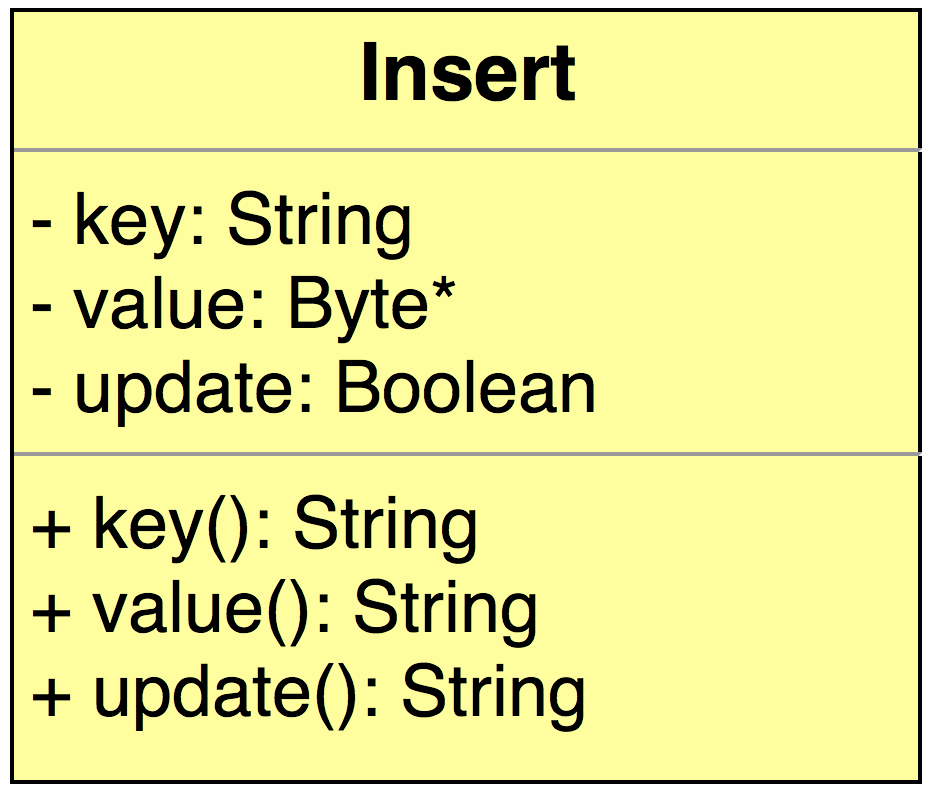
\includegraphics[width=0.3\textwidth,keepaspectratio]{RA/insert.png}
    \caption{Classe Insert}
  \end{center}
\end{figure}

\subparagraph{Descrizione}

Classe che rappresenta un messaggio utilizzato per richiedere l'aggiunta di un item.\\Implementata utilizzando la specifica funzionalità \textit{case class} di Scala,
in modo da poter usufruirne mediante costrutti e algoritmi di
\gloss{pattern matching}.

\subparagraph{Utilizzo}

Questa classe viene utilizzata per richiedere l'aggiunta di un item dal
sistema.\\Quando riceve questo messaggio l'attore provvederà a inoltrare la
richiesta allo
\hyperref[sec:actorbase::actorsystem::actors::storekeeper::Storekeeper]{Storekeeper}
giusto.

\subparagraph{Attributi}
\begin{tabular}{| p{2cm} | p{1.5cm} | p{2cm} | p{3cm} | p{8.5cm} |}
  \hline
  Nome & Accesso & Mutabilità & Tipo & Descrizione\\
  \hline
  key & pubblico & immutabile & String & Rappresenta la chiave dell'elemento da aggiungere dalla collezione rappresentata da questo attore\\
  \hline
  value & pubblico & immutabile & Array<Byte> & Rappresenta il valore dell'item da inserire sotto forma di array di bytes\\
  \hline
  update & pubblico & immutabile & Boolean & Rappresenta un flag che server a scegliere se l'operazione può effettuare sovrascrittura o no (true se l'operazione può sovrascrivere items con la stessa chiave)\\
  \hline
\end{tabular}

\subparagraph{Metodi}
\begin{tabular}{| p{3cm} | p{1.5cm} | p{3.5cm} | p{9cm} |}
  \hline
  Nome & Accesso & Tipo di ritorno & Descrizione\\
  \hline
  key & pubblico & String & Metodo che ritorna l'attributo key\\
  \hline
  value & pubblico & Array<Byte> & Metodo che ritorna l'attributo value\\
  \hline
  update & pubblico & Boolean & Metodo che ritorna l'attributo update\\
  \hline
\end{tabular}

%%%%%%%%%%%%%%%%%%%%%%%%%%%%%%%%%%%%%%%%%%%%%%%%%%%%%%%%%%%%%%%%%%%%%%%%%

\subsection{actorbase::actorsystem::messages::storekeepermessages}
\label{sec:actorbase::actorsystem::messages::storekeepermessages}

% TODO img
\begin{figure}[H]
  \begin{center}
    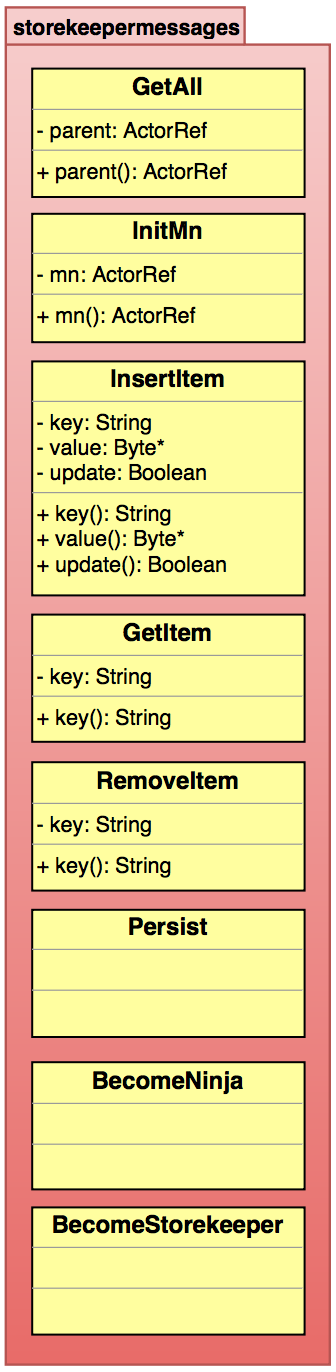
\includegraphics[width=0.6\textwidth,keepaspectratio]{RA/storekeepermessages.png}
    \caption{Package actorsystem::messages::storekeepermessages}
  \end{center}
\end{figure}

\subsubsection{Descrizione}
\gloss{Package} contenente i messaggi processabili dall'attore \hyperref[sec:actorbase::actorsystem::actors::storekeeper::Storekeeper]{Storekeeper}.

\subsubsection{Classi}

\paragraph{actorbase::actorsystem::messages::storekeeper::Persist}
\label{sec:actorbase::actorsystem::messages::storekeeper::Persist}

% TODO img
\begin{figure}[H]
  \begin{center}
    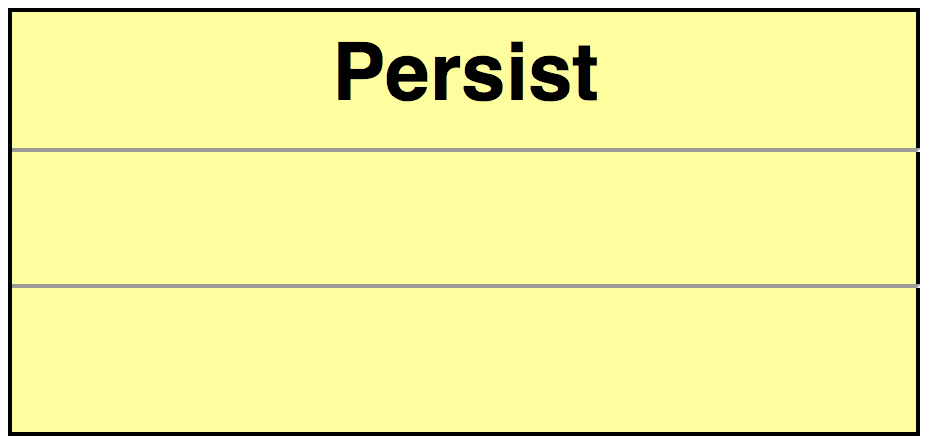
\includegraphics[width=0.3\textwidth,keepaspectratio]{RA/persist.png}
    \caption{Classe Persist}
  \end{center}
\end{figure}

\subparagraph{Descrizione}
Classe che rappresenta un messaggio utilizzato per richiedere allo
\hyperref[sec:actorbase::actorsystem::actors::storekeeper::Storekeeper]{Storekeeper} di persistere i dati su disco.\\Implementata utilizzando la specifica funzionalità \textit{case class} di Scala,
in modo da poter usufruirne mediante costrutti e algoritmi di
\gloss{pattern matching}.

\subparagraph{Utilizzo}
Questa classe viene utilizzata per richiedere di effettuare persistenza su disco dei dati di questo attore.\\Questo attore provvederà a inoltrare la richiesta
all'attore \hyperref[sec:actorbase::actorsystem::actors::warehouseman::Warehouseman]{Warehouseman}.

\paragraph{actorbase::actorsystem::messages::storekeeper::InitMn}
\label{sec:actorbase::actorsystem::messages::storekeeper::InitMn}

% TODO img
\begin{figure}[H]
  \begin{center}
    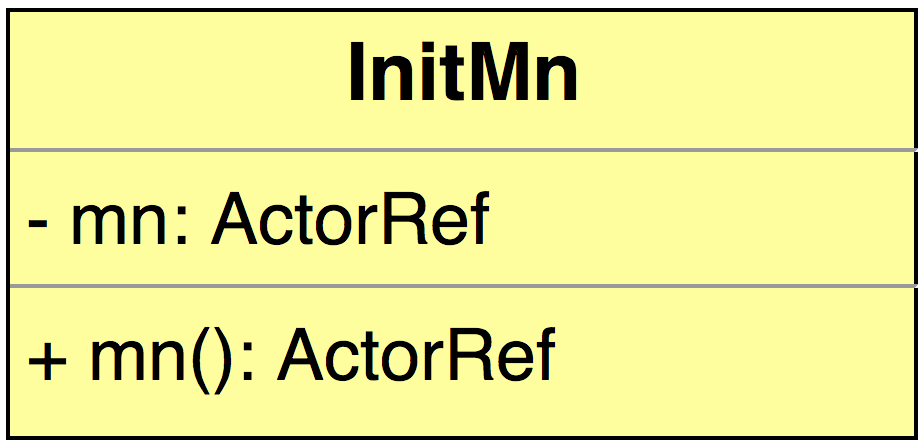
\includegraphics[width=0.3\textwidth,keepaspectratio]{RA/InitMn.png}
    \caption{Classe InitMn}
  \end{center}
\end{figure}

\subparagraph{Descrizione}
Classe che rappresenta un messaggio utilizzato per inizializzare un riferimento ad un attore \hyperref[sec:actorbase::actorsystem::actors::manager::Manager]{Manager}.\\Implementata utilizzando la specifica funzionalità \textit{case class} di Scala,
in modo da poter usufruirne mediante costrutti e algoritmi di
\gloss{pattern matching}.

\subparagraph{Utilizzo}
Questa classe viene utilizzata per ricevere un riferimento ad un attore
\hyperref[sec:actorbase::actorsystem::actors::manager::Manager]{Manager}.
Questo messaggio verrà inviato allo \hyperref[sec:actorbase::actorsystem::actors::storekeeper::Storekeeper]{Storekeeper}
subito dopo la sua creazione.\\L'attore userà il riferimento al \hyperref[sec:actorbase::actorsystem::actors::manager::Manager]{Manager} per
informarlo quando raggiunge una certa soglia di items. Il \hyperref[sec:actorbase::actorsystem::actors::manager::Manager]{Manager} creerà altri
\hyperref[sec:actorbase::actorsystem::actors::storekeeper::Storekeeper]{Storekeeper} per distribuire il carico.

\subparagraph{Attributi}
\begin{tabular}{| p{2cm} | p{1.5cm} | p{2cm} | p{3cm} | p{8.5cm} |}
  \hline
  Nome & Accesso & Mutabilità & Tipo & Descrizione\\
  \hline
  mn & pubblico & immutabile & ActorRef & Rappresenta un riferimento ad un attore \hyperref[sec:actorbase::actorsystem::actors::manager::Manager]{Manager}\\
  \hline
\end{tabular}

\subparagraph{Metodi}
\begin{tabular}{| p{3cm} | p{1.5cm} | p{3.5cm} | p{9cm} |}
  \hline
  Nome & Accesso & Tipo di ritorno & Descrizione\\
  \hline
  man & pubblico & ActorRef & Metodo che ritorna l'attributo mn\\
  \hline
\end{tabular}

\paragraph{actorbase::actorsystem::messages::storekeeper::GetAll}
\label{sec:actorbase::actorsystem::messages::storekeeper::GetAll}

% TODO img
\begin{figure}[H]
  \begin{center}
    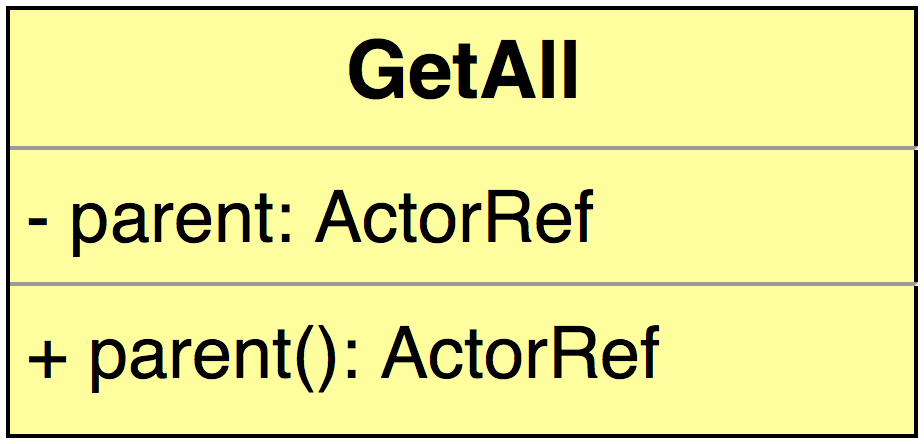
\includegraphics[width=0.3\textwidth,keepaspectratio]{RA/getAll.png}
    \caption{Classe GetAll}
  \end{center}
\end{figure}

\subparagraph{Descrizione}
Classe che rappresenta un messaggio utilizzato per richiedere tutti gli items
contenuti nell'attore.\\Implementata utilizzando la specifica funzionalità \textit{case class} di Scala,
in modo da poter usufruirne mediante costrutti e algoritmi di
\gloss{pattern matching}.

\subparagraph{Utilizzo}
Questa classe viene utilizzata per ricevere una richiesta di restituzione di
tutti gli items mappati da questo attore.\\Quando questo attore riceve questo
messaggio provvederà a inviare tutti gli items contenuti in esso al riferimento
all'attore passato come parametro.\\Questo messaggio serve a
restituire all'utente intere collezioni.

\subparagraph{Attributi}
\begin{tabular}{| p{2cm} | p{1.5cm} | p{2cm} | p{3cm} | p{8.5cm} |}
  \hline
  Nome & Accesso & Mutabilità & Tipo & Descrizione\\
  \hline
  parent & pubblico & immutabile & ActorRef & Rappresenta un riferimento all'attore \hyperref[sec:actorbase::actorsystem::actors::storefinder::Storefinder]{Storefinder} che rappresenta la collezione di cui lo \hyperref[sec:actorbase::actorsystem::actors::storekeeper::Storekeeper]{Storekeeper} fa parte\\
  \hline
\end{tabular}

\subparagraph{Metodi}
\begin{tabular}{| p{3cm} | p{1.5cm} | p{3.5cm} | p{9cm} |}
  \hline
  Nome & Accesso & Tipo di ritorno & Descrizione\\
  \hline
  parent & pubblico & ActorRef & Metodo che ritorna l'attributo parent\\
  \hline
\end{tabular}

\paragraph{actorbase::actorsystem::messages::storekeeper::GetItem}
\label{sec:actorbase::actorsystem::messages::storekeeper::GetItem}

% TODO img
\begin{figure}[H]
  \begin{center}
    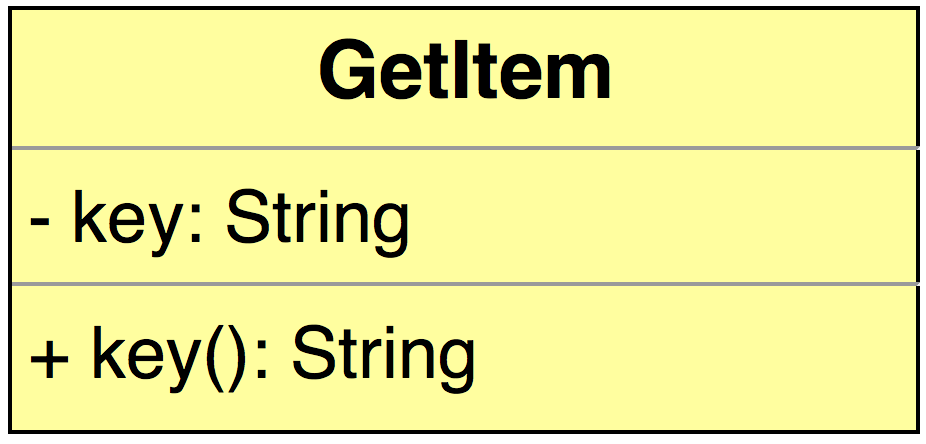
\includegraphics[width=0.3\textwidth,keepaspectratio]{RA/getItem.png}
    \caption{Classe GetItem}
  \end{center}
\end{figure}

\subparagraph{Descrizione}
Classe che rappresenta un messaggio utilizzato per richiedere un item
contenuto nell'attore.\\Implementata utilizzando la specifica funzionalità \textit{case class} di Scala,
in modo da poter usufruirne mediante costrutti e algoritmi di
\gloss{pattern matching}.

\subparagraph{Utilizzo}
Questa classe viene utilizzata per richiedere la restituzione di un
item mappato da questo attore.\\Quando questo attore riceve questo
messaggio provvederà a inviare l'item richiesto all'attore \hyperref[sec:actorbase::actorsystem::actors::clientactor::ClientActor]{ClientActor} che
ha effettuato la richiesta.

\subparagraph{Attributi}
\begin{tabular}{| p{2cm} | p{1.5cm} | p{2cm} | p{3cm} | p{8.5cm} |}
  \hline
  Nome & Accesso & Mutabilità & Tipo & Descrizione\\
  \hline
  key & pubblico & immutabile & String & Rappresenta la chiave dell'item da restituire\\
  \hline
\end{tabular}

\subparagraph{Metodi}
\begin{tabular}{| p{3cm} | p{1.5cm} | p{3.5cm} | p{9cm} |}
  \hline
  Nome & Accesso & Tipo di ritorno & Descrizione\\
  \hline
  key & pubblico & String & Metodo che ritorna l'attributo key\\
  \hline
\end{tabular}

\paragraph{actorbase::actorsystem::messages::storekeeper::InsertItem}
\label{sec:actorbase::actorsystem::messages::storekeeper::InsertItem}

% TODO img
\begin{figure}[H]
  \begin{center}
    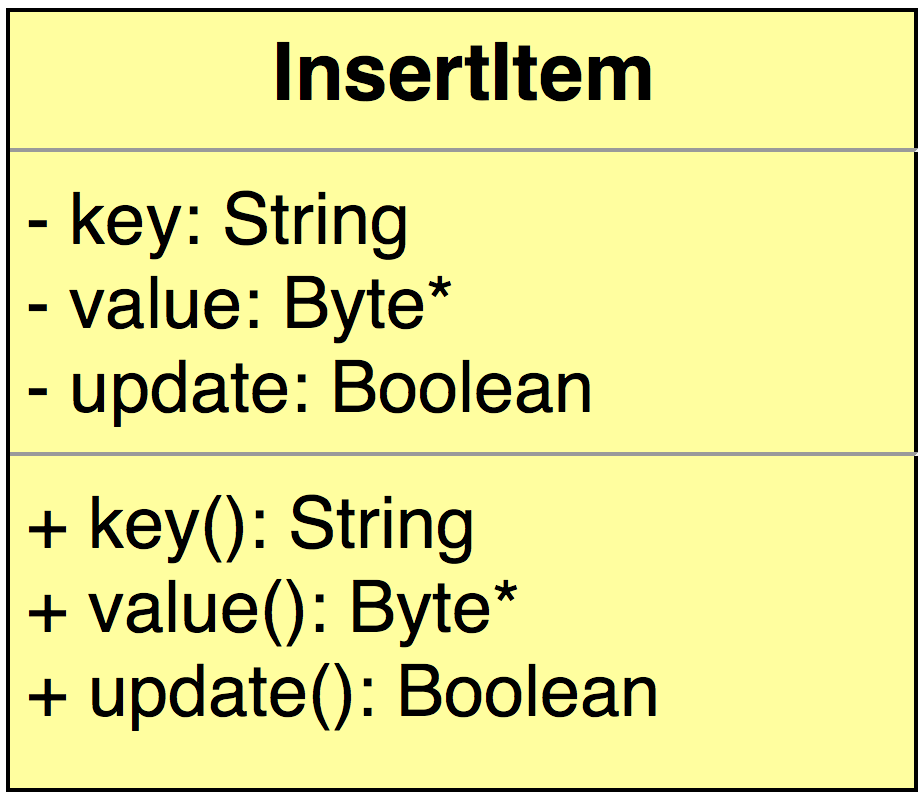
\includegraphics[width=0.3\textwidth,keepaspectratio]{RA/insertItem.png}
    \caption{Classe InsertItem}
  \end{center}
\end{figure}

\subparagraph{Descrizione}
Classe che rappresenta un messaggio utilizzato per richiedere l'inserimento di
un item.\\Implementata utilizzando la specifica funzionalità \textit{case class} di Scala,
in modo da poter usufruirne mediante costrutti e algoritmi di
\gloss{pattern matching}.

\subparagraph{Utilizzo}
Questa classe viene utilizzata per richiedere l'inserimento di un item.\\Quando questo attore riceve questo messaggio provvederà ad aggiungere l'item in
questione nella propria struttura dati.\\L'inserimento può avvenire con
sovrascrittura o senza a seconda del valore dell'attributo update passato nel
messaggio.

\subparagraph{Attributi}
\begin{tabular}{| p{2cm} | p{1.5cm} | p{2cm} | p{3cm} | p{8.5cm} |}
  \hline
  Nome & Accesso & Mutabilità & Tipo & Descrizione\\
  \hline
  key & pubblico & immutabile & String & Rappresenta la chiave dell'item da inserire\\
  \hline
  value & pubblico & immutabile & Array<Byte> & Rappresenta il valore dell'item in formato array di bytes\\
  \hline
  update & pubblico & immutabile & Boolean & Flag per scegliere se l'inserimento può effettuare sovrascrittura o meno (true se può effettuare sovrascrittura)\\
  \hline
\end{tabular}

\subparagraph{Metodi}
\begin{tabular}{| p{3cm} | p{1.5cm} | p{3.5cm} | p{9cm} |}
  \hline
  Nome & Accesso & Tipo di ritorno & Descrizione\\
  \hline
  key & pubblico & String & Metodo che ritorna l'attributo key\\
  \hline
  value & pubblico & Array<Byte> & Metodo che ritorna l'attributo value\\
  \hline
  update & pubblico & Boolean & Metodo che ritorna l'attributo update\\
  \hline
\end{tabular}

\paragraph{actorbase::actorsystem::messages::storekeeper::RemoveItem}
\label{sec:actorbase::actorsystem::messages::storekeeper::RemoveItem}

% TODO img
\begin{figure}[H]
  \begin{center}
    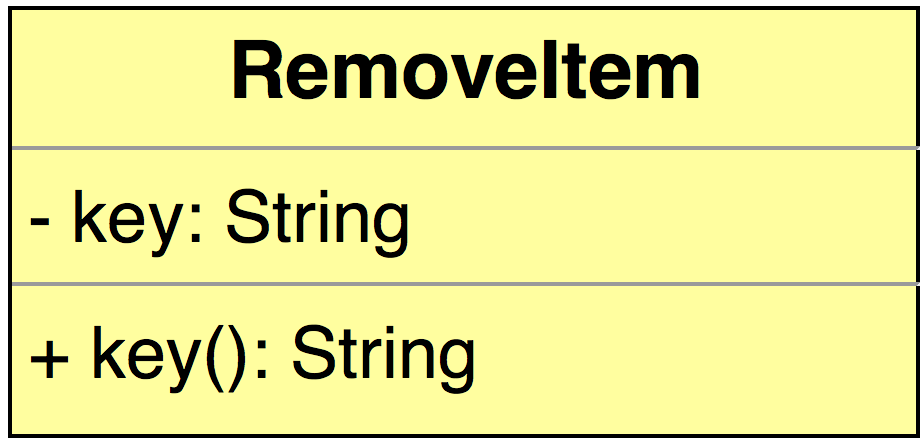
\includegraphics[width=0.3\textwidth,keepaspectratio]{RA/removeItem.png}
    \caption{Classe RemoveItem}
  \end{center}
\end{figure}

\subparagraph{Descrizione}
Classe che rappresenta un messaggio utilizzato per richiedere la rimozione di un
item contenuto nell'attore.\\Implementata utilizzando la specifica funzionalità
\textit{case class} di Scala,
in modo da poter usufruirne mediante costrutti e algoritmi di
\gloss{pattern matching}.

\subparagraph{Utilizzo}
Questa classe viene utilizzata per richiedere la rimozione di un
item mappato da questo attore.\\Quando questo attore riceve questo
messaggio provvederà a rimuovere dalla propria struttura dati l'item con la
chiave passata come parametro.

\subparagraph{Attributi}
\begin{tabular}{| p{2cm} | p{1.5cm} | p{2cm} | p{3cm} | p{8.5cm} |}
  \hline
  Nome & Accesso & Mutabilità & Tipo & Descrizione\\
  \hline
  key & privato & immutabile & String & Rappresenta la chiave dell'item da rimuovere\\
  \hline
\end{tabular}

\subparagraph{Metodi}
\begin{tabular}{| p{3cm} | p{1.5cm} | p{3.5cm} | p{9cm} |}
  \hline
  Nome & Accesso & Tipo di ritorno & Descrizione\\
  \hline
  key & pubblico & String & Metodo che ritorna l'attributo key\\
  \hline
\end{tabular}

%%%%%%%%%%%%%%%%%%%%%%%%%%%%%%%%%%%%%%%%%%%%%%%%%%%%%%%%%%%%%%%%%%%%%%%%%

\subsection{actorbase::actorsystem::messages::warehousemanmessages}
\label{sec:actorbase::actorsystem::messages::warehousemanmessages}

% TODO img
\begin{figure}[H]
  \begin{center}
    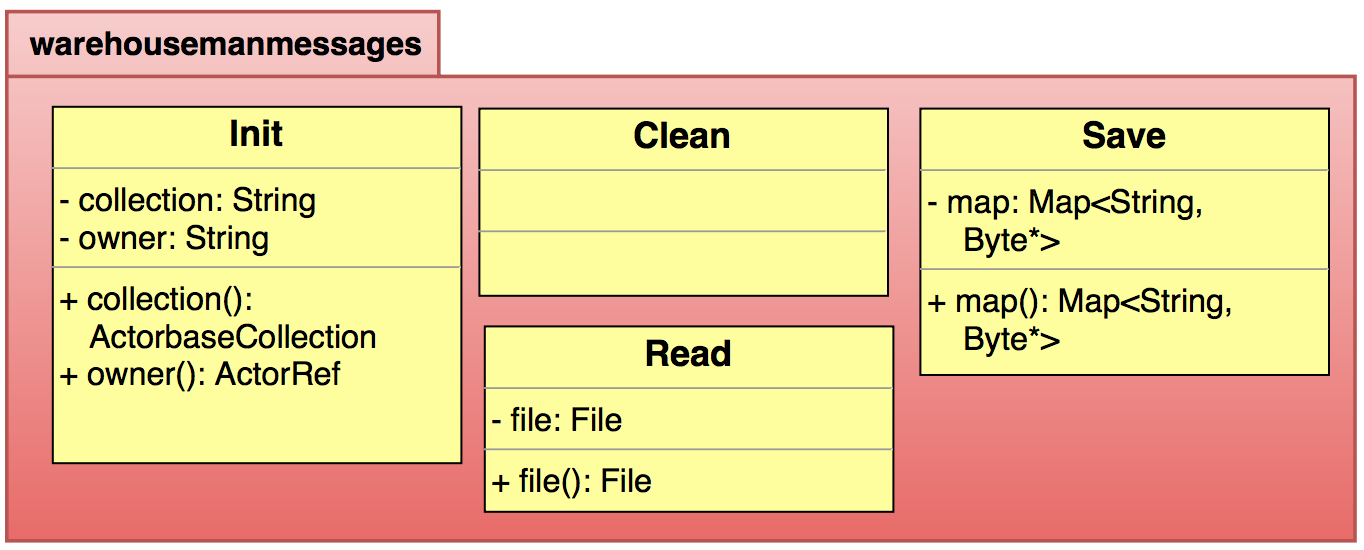
\includegraphics[width=0.8\textwidth,keepaspectratio]{RA/warehousemanmessages.png}
    \caption{Package actorsystem::messages::warehousemanmessages}
  \end{center}
\end{figure}

\subsubsection{Descrizione}
\gloss{Package} contenente i messaggi processabili dall'attore \hyperref[sec:actorbase::actorsystem::actors::warehouseman::Warehouseman]{Warehouseman}.

\subsubsection{Classi}

\paragraph{actorbase::actorsystem::messages::warehouseman::Clean}
\label{sec:actorbase::actorsystem::messages::warehouseman::Clean}

% TODO img
\begin{figure}[H]
  \begin{center}
    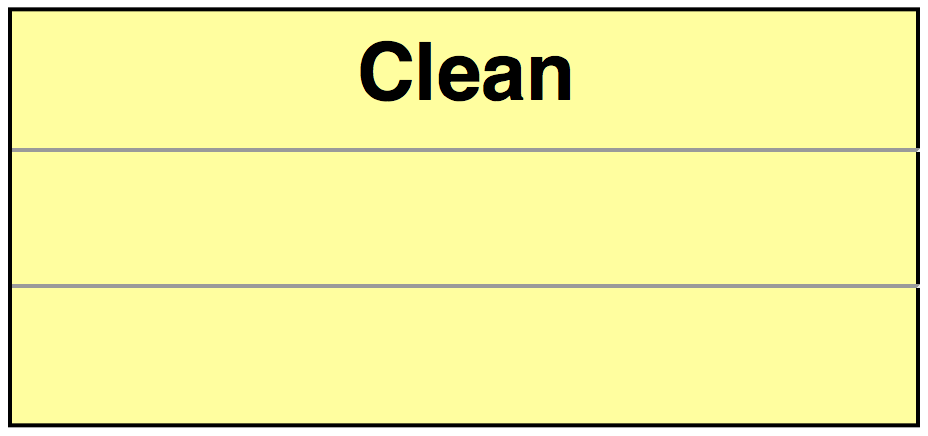
\includegraphics[width=0.3\textwidth,keepaspectratio]{RA/clean.png}
    \caption{Classe Clean}
  \end{center}
\end{figure}

\subparagraph{Descrizione}
Classe che rappresenta un messaggio utilizzato per richiedere allo
\hyperref[sec:actorbase::actorsystem::actors::warehouseman::Warehouseman]{Warehouseman} di rimuovere i dati rappresentati da esso dal disco.\\Implementata utilizzando la specifica funzionalità \textit{case class} di Scala,
in modo da poter usufruirne mediante costrutti e algoritmi di
\gloss{pattern matching}.

\subparagraph{Utilizzo}
Questa classe viene utilizzata per richiedere di rimuovere dal disco tutti i
file contenenti dati rappresentati dall'attore in questione.\\Questo messaggio
è utilizzato ad esempio quando si rimuove una collezione dal sistema.

\paragraph{actorbase::actorsystem::messages::warehouseman::Init}
\label{sec:actorbase::actorsystem::messages::warehouseman::Init}

% TODO img
\begin{figure}[H]
  \begin{center}
    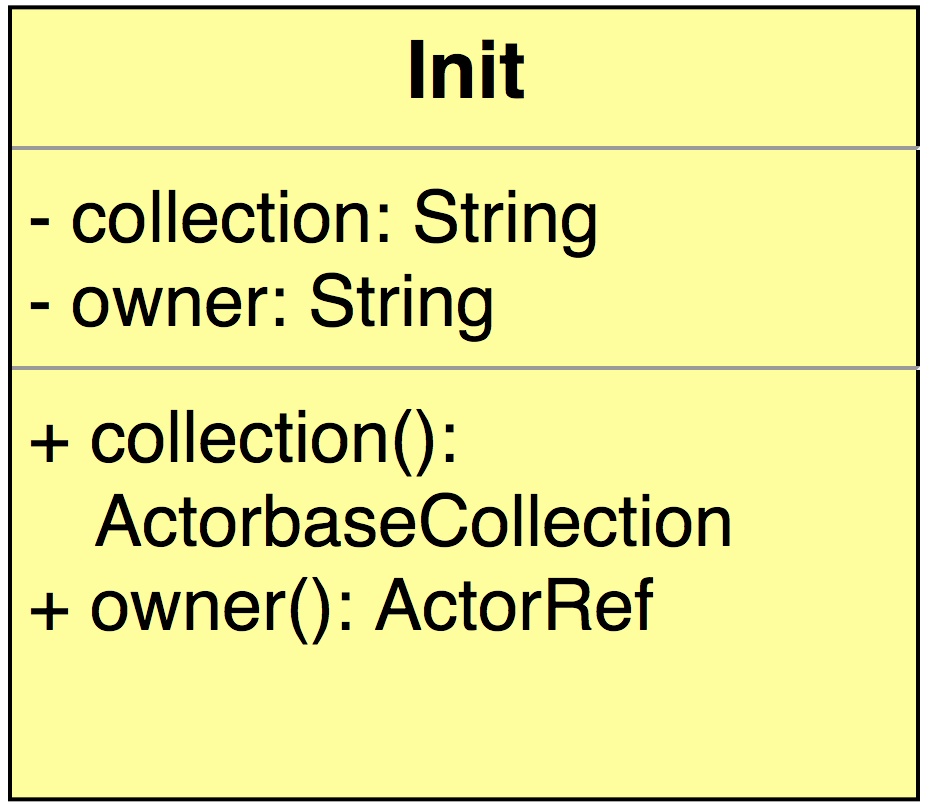
\includegraphics[width=0.3\textwidth,keepaspectratio]{RA/init.png}
    \caption{Classe Init}
  \end{center}
\end{figure}

\subparagraph{Descrizione}
Classe che rappresenta un messaggio utilizzato per inizializzare l'attore.\\Implementata utilizzando la specifica funzionalità \textit{case class} di Scala,
in modo da poter usufruirne mediante costrutti e algoritmi di
\gloss{pattern matching}.

\subparagraph{Utilizzo}
Questa classe viene utilizzata per inizializzare l'attore con le informazioni
necessarie come la collezione che rappresenta.\\Questo messaggio viene
ricevuto subito dopo la propria creazione in modo da inizializzarlo immediatamente.

\subparagraph{Attributi}
\begin{tabular}{| p{2cm} | p{1.5cm} | p{2cm} | p{3cm} | p{8.5cm} |}
  \hline
  Nome & Accesso & Mutabilità & Tipo & Descrizione\\
  \hline
  collection & privato & immutabile & String & Rappresenta il nome della collezione che questo attore rappresenta\\
  \hline
  owner & privato & immutable & String & Rappresenta lo username dell'utente che ha creato la collezione che questo attore rappresenta\\
  \hline
\end{tabular}

\subparagraph{Metodi}
\begin{tabular}{| p{3cm} | p{1.5cm} | p{3.5cm} | p{9cm} |}
  \hline
  Nome & Accesso & Tipo di ritorno & Descrizione\\
  \hline
  collection & pubblico & String & Metodo che ritorna l'attributo collection\\
  \hline
  owner & pubblico & String & Metodo che ritorna l'attributo owner\\
  \hline
\end{tabular}

\paragraph{actorbase::actorsystem::messages::warehouseman::Save}
\label{sec:actorbase::actorsystem::messages::warehouseman::Save}

% TODO img
\begin{figure}[H]
  \begin{center}
    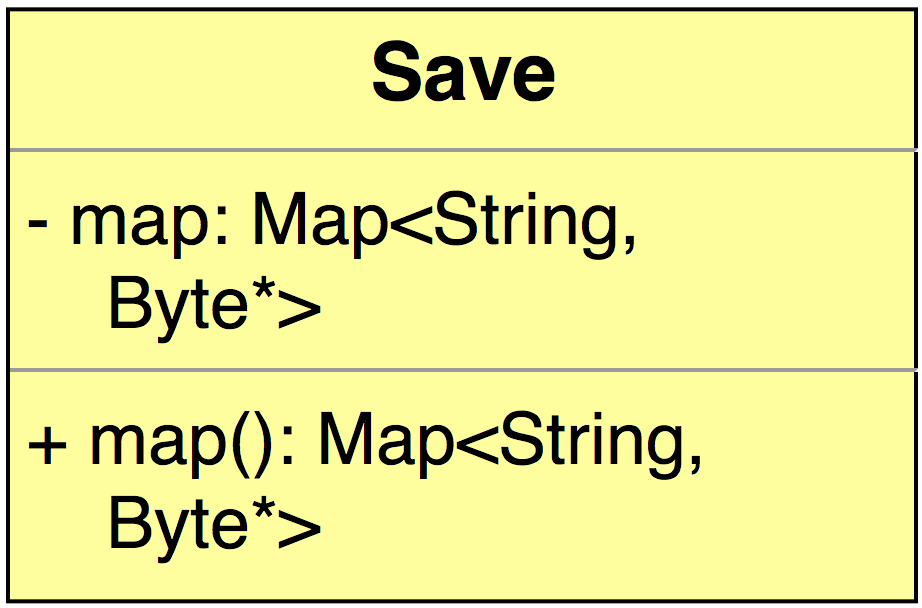
\includegraphics[width=0.3\textwidth,keepaspectratio]{RA/save.png}
    \caption{Classe Save}
  \end{center}
\end{figure}

\subparagraph{Descrizione}
Classe che rappresenta un messaggio utilizzato per persistere i dati su disco.\\Implementata utilizzando la specifica funzionalità \textit{case class} di Scala,
in modo da poter usufruirne mediante costrutti e algoritmi di
\gloss{pattern matching}.

\subparagraph{Utilizzo}
Questa classe viene utilizzata per richiedere all'attore di persistere dati
su disco. Quando l'attore riceve questo messaggio provvederà a salvare su
filesystem i dati passati come parametri in file che seguono una gerarchia
simile alla gerarchia delle collezioni del sistema.\\I dati salvati vengono prima criptati tramite l'ausilio della classe \hyperref[sec:actorbase::actorsystem::utils::CryptoUtils]{CryptoUtils}

\subparagraph{Attributi}
\begin{tabular}{| p{2cm} | p{1.5cm} | p{2cm} | p{3cm} | p{8.5cm} |}
  \hline
  Nome & Accesso & Mutabilità & Tipo & Descrizione\\
  \hline
  map & privato & immutable & Map<String, Array<Byte> > & Rappresenta una mappa di items da salvare su disco\\
  \hline
\end{tabular}

\subparagraph{Metodi}
\begin{tabular}{| p{3cm} | p{1.5cm} | p{3.5cm} | p{9cm} |}
  \hline
  Nome & Accesso & Tipo di ritorno & Descrizione\\
  \hline
  map & pubblico & Map<String, Array<Byte> > & Metodo che ritorna l'attributo map\\
  \hline
\end{tabular}

\paragraph{actorbase::actorsystem::messages::warehouseman::Read}
\label{sec:actorbase::actorsystem::messages::warehouseman::Read}

% TODO img
\begin{figure}[H]
  \begin{center}
    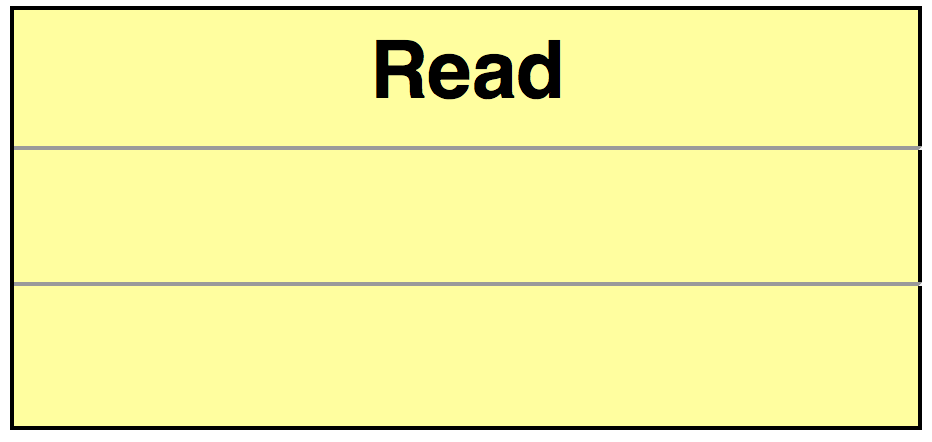
\includegraphics[width=0.3\textwidth,keepaspectratio]{RA/read.png}
    \caption{Classe Read}
  \end{center}
\end{figure}

\subparagraph{Descrizione}
Classe che rappresenta un messaggio utilizzato per leggere i dati da disco.\\Implementata utilizzando la specifica funzionalità \textit{case class} di Scala,
in modo da poter usufruirne mediante costrutti e algoritmi di
\gloss{pattern matching}.

\subparagraph{Utilizzo}
Questa classe viene utilizzata per richiedere all'attore di leggere dati
da disco. Quando l'attore riceve questo messaggio provvederà a decriptare,
leggere e restituire i dati all'attore richiedente.\\Questo messaggio è usato ad esempio quando il sistema subisce un riavvio per ripopolare la struttura coi dati scritti su disco.

\subparagraph{Attributi}
\begin{tabular}{| p{2cm} | p{1.5cm} | p{2cm} | p{3cm} | p{8.5cm} |}
  \hline
  Nome & Accesso & Mutabilità & Tipo & Descrizione\\
  \hline
  file & privato & immutable & File & Rappresenta un file da cui leggere gli items\\
  \hline
\end{tabular}

\subparagraph{Metodi}
\begin{tabular}{| p{3cm} | p{1.5cm} | p{3.5cm} | p{9cm} |}
  \hline
  Nome & Accesso & Tipo di ritorno & Descrizione\\
  \hline
  file & pubblico & File & Metodo che ritorna l'attributo file\\
  \hline
\end{tabular}

\subsection{actorbase::actorsystem::messages::managermessages}
\label{sec:actorbase::actorsystem::messages::managermessages}

% TODO img
\begin{figure}[H]
  \begin{center}
    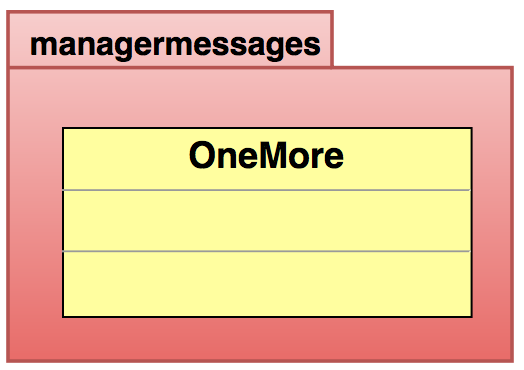
\includegraphics[width=0.4\textwidth,keepaspectratio]{RA/managermessages.png}
    \caption{Package actorsystem::messages::managermessages}
  \end{center}
\end{figure}

\subsubsection{Descrizione}
\gloss{Package} contenente i messaggi processabili dall'attore
\hyperref[sec:actorbase::actorsystem::actors::manager::Manager]{Manager}.

\subsubsection{Classi}

\paragraph{actorbase::actorsystem::messages::managermessages::OneMore}

% TODO img
\begin{figure}[H]
  \begin{center}
    \includegraphics[width=0.3\textwidth,keepaspectratio]{RA/oneMore.png}
    \caption{Classe OneMore}
  \end{center}
\end{figure}

\subparagraph{Descrizione}
Classe che rappresenta un messaggio utilizzato per alleggerire il carico in
ingresso degli \gloss{attori} di tipo
\hyperref[sec:actorbase::actorsystem::actors::storekeeper::Storekeeper]{Storekeeper},
creandone di nuovi e aggiungendoli alla \gloss{pool} dell'\gloss{attore} di tipo
\hyperref[sec:actorbase::actorsystem::actors::storefinder::Storefinder]{Storefinder}
che li coordina.

\subparagraph{Utilizzo}
Viene utilizzato dagli \gloss{attori} di tipo
\hyperref[sec:actorbase::actorsystem::actors::Storekeeper]{Storekeeper} per
notificare il superamento della soglia di coppie chiave-valore impostata da
configurazione, che determina quindi un sovraccarico dell'\gloss{attore} in
questione.\\ Il messaggio si occupa dunque di generare nuovi \gloss{attori} di
tipo
\hyperref[sec:actorbase::actorsystem::actors::storekeeper::Storekeeper]{Storekeeper}
in modo da redistribuire il carico in ingresso.


%%%%%%%%%%%%%%%%%%%%%%%%%%%%%%%%%%%%%%%%%%%%%%%%%%%%%%%%%%%%%%%%%%%%%%%%%
%%%%%%%%%%%%%%%%%%%%%%%%%%%%%%%%%%%%%%%%%%%%%%%%%%%%%%%%%%%%%%%%%%%%%%%%%
%%%%% ACTORS PARTE %%%%
%%%%%%%%%%%%%%%%%%%%%%%%%%%%%%%%%%%%%%%%%%%%%%%%%%%%%%%%%%%%%%%%%%%%%%%%%

\subsection{actorbase::actorsystem::actors} %TODO apposto sto package?
\label{sec:actorbase::actorsystem::actors}

\begin{figure}[H]
  \begin{center}
    \includegraphics[width=0.8\textwidth,keepaspectratio]{RA/Actors.png}
    \caption{\gloss{Package} actors, visione generale}
  \end{center}
\end{figure}

\subsubsection{Descrizione}

\gloss{Package} che raggruppa tutti gli attori necessari al funzionamento del database.

\subsubsection{Package contenuti}
\begin{itemize}
\item \hyperref[sec:actorbase::actorsystem::actors::clientactor]{actorbase::actorsystem::actors::clientactor};
\item \hyperref[sec:actorbase::actorsystem::actors::httpserver]{actorbase::actorsystem::actors::httpserver};
\item \hyperref[sec:actorbase::actorsystem::actors::storefinder]{actorbase::actorsystem::actors::storefinder};
\item \hyperref[sec:actorbase::actorsystem::actors::storekeeper]{actorbase::actorsystem::actors::storekeeper};
\item \hyperref[sec:actorbase::actorsystem::actors::warehouseman]{actorbase::actorsystem::actors::warehouseman};
\item \hyperref[sec:actorbase::actorsystem::actors::manager]{actorbase::actorsystem::actors::manager};
\item \hyperref[sec:actorbase::actorsystem::actors::main]{actorbase::actorsystem::actors::main};
\item \hyperref[sec:actorbase::actorsystem::actors::authactor]{actorbase::actorsystem::actors::authactor}.
\end{itemize}

\subsection{actorbase::actorsystem::actors::clientactor}
\label{sec:actorbase::actorsystem::actors::clientactor}

\begin{figure}[H]
  \begin{center}
    \includegraphics[width=0.7\textwidth,keepaspectratio]{RA/clientactorPackage.png}
    \caption{\gloss{Package} Clientactor e interazioni con Main}
  \end{center}
\end{figure}

\subsubsection{Descrizione}

\gloss{Package} per l'\gloss{attore} con cui si interfaccerà il \gloss{driver},
fornisce un'interfaccia \gloss{HTTP} verso l'esterno.

\subsubsection{Classi}

\paragraph{actorbase::actorsystem::actors::clientactor::Authenticator}
\label{sec:actorbase::actorsystem::actors::clientactor::Authenticator}

\begin{figure}[H]
  \begin{center}
    \includegraphics[width=0.5\textwidth,keepaspectratio]{RA/authenticator.png}
    \caption{Classe actorsystem::actors::clientactor::Authenticator}
  \end{center}
\end{figure}

\subparagraph{Descrizione}

Classe astratta usata per effettuare la validazione di un login.

\subparagraph{Utilizzo}

Questa classe viene usata dalla classe che la realizza per effettuare il
controllo delle credenziali di login mediante richiesta all'\gloss{attore} di
tipo
\hyperref[sec:actorbase::actorsystem::actors::authactor::AuthActor]{AuthActor}.

\subparagraph{Metodi}

\begin{tabular}{| p{4cm} | p{1.5cm} | p{4cm} | p{7.5cm} |}
  \hline
  Nome & Accesso & Tipo di ritorno & Descrizione\\
  \hline
  basicUserAuthenticator & pubblico & AuthMagnet[AuthInfo] & Metodo che riceve e controlla tramite metodi interni le credenziali\\
  \hline
  validateUser & pubblico & Option[AuthInfo] & Metodo che controlla che le credenziali siano corrette\\
  \hline
  authenticator & pubblico & Future[Option[AuthInfo]] & Metodo che restituisce un \gloss{future} che punta alle credenziali dell'utente autenticato\\
  \hline
\end{tabular}

\subparagraph{Parametri}

\textbf{basicUserAuthenticator}\\ \\
\begin{tabular}{| p{2cm} | p{3cm} | p{12cm} |}
  \hline
  Nome & Tipo & Descrizione\\
  \hline
  ec & ExecutionContext & Contesto di esecuzione all'interno del quale è stato chiamato questo metodo\\
  \hline
  authProxy & ActorRef & Riferimento dell'\gloss{attore} di tipo \hyperref[sec:actorbase::actorsystem::actors::authactor::AuthActor]{AuthActor} che si occuperà di validare le credenziali di accesso al sistema\\
  \hline
\end{tabular}\\

\textbf{validateUser}\\ \\
\begin{tabular}{| l | l | l |}
  \hline
  Nome & Tipo & Descrizione\\
  \hline
  userPass & Option[UserPass] & Credenziali di accesso dell'utente che vuole autenticarsi\\
  \hline
\end{tabular}\\

\textbf{authenticator}\\ \\
\begin{tabular}{| l | l | l |}
  \hline
  Nome & Tipo & Descrizione\\
  \hline
  userPass & Option[UserPass] & Credenziali di accesso dell'utente che vuole autenticarsi\\
  \hline
\end{tabular}\\

% \paragraph{actorbase::actorsystem::actors::clientactor::ItemApi}
% \label{sec:actorbase::actorsystem::actors::clientactor::ItemApi}

% \begin{figure}[H]
%   \begin{center}
%     \includegraphics[width=0.5\textwidth,keepaspectratio]{RA/itemapi.png}
%     \caption{Classe actorsystem::actors::clientactor::ItemApi}
%   \end{center}
% \end{figure}

% \subparagraph{Descrizione}

% Classe astratta usata per analizzare le route che richiedono operazioni su item.

% \subparagraph{Utilizzo}

% Questa classe viene usata dalla classe che la realizza per effettuare l'analisi
% delle route che richiedono operazioni su item.

% \subparagraph{Attributi}
% \begin{tabular}{| p{1cm} | p{1.5cm} | p{2cm} | p{4cm} | p{8.5cm} |}
%   \hline
%   Nome & Accesso & Mutabilità & Tipo & Descrizione\\
%   \hline
%   ec & pubblico & immutabile & ExecutionContext & Rappresenta il Contesto di esecuzione all'interno del quale è stata creata questa classe \\
%   \hline
% \end{tabular}

% \subparagraph{Metodi}

% \begin{tabular}{| p{2.5cm} | p{2.5cm} | p{2.5cm} | p{9.5cm} |}
%   \hline
%   Nome & Accesso & Tipo di ritorno & Descrizione\\
%   \hline
%   items & pubblico & Route & Metodo che interagisce con il server tramite un router basandosi sulla route immessa dall'utente\\
%   \hline
% \end{tabular}

% \subparagraph{Parametri}

% \textbf{items}\\ \\
% \begin{tabular}{| p{2.5cm} | p{2.5cm} | p{12cm} |}
%   \hline
%   Nome & Tipo & Descrizione\\
%   \hline
%   owner & String & Proprietario della \gloss{collezione} su cui si vuole operare\\
%   \hline
%   router & ActorRef & Riferimento dell'attore che si occuperà di comunicare con un attore \gloss{main} per effettuare le operazioni richieste\\
%   \hline
%   collectionName & String & Nome della \gloss{collezione} su cui si vuole operare\\
%   \hline
% \end{tabular}\\

\paragraph{actorbase::actorsystem::actors::clientactor::User}
\label{sec:actorbase::actorsystem::actors::clientactor::User}

\begin{figure}[H]
  \begin{center}
    \includegraphics[width=0.3\textwidth,keepaspectratio]{RA/user.png}
    \caption{Classe actorsystem::actors::clientactor::User}
  \end{center}
\end{figure}

\subparagraph{Descrizione}

Classe che rappresenta un utente collegato e autenticato dall'esterno al sistema
mediante richiesta di \gloss{login}.

\subparagraph{Utilizzo}

Questa classe viene usata per fornire le informazioni di autenticazione
all'\gloss{attore} di tipo
\hyperref[sec:actorbase::actorsystem::actors::clientactor::ClientActor]{ClientActor}
una volta ottenuta la validazione da parte
dell'\hyperref[sec:actorbase::actorsystem::actors::clientactor::Authenticator]{Authenticator}, mediante
oggetto di tipo \hyperref[sec:actorbase::actorsystem::actors::clientactor::AuthInfo]{AuthInfo}.

\subparagraph{Attributi}
\begin{tabular}{| p{1.5cm} | p{1.5cm} | p{2cm} | p{3cm} | p{8.5cm} |}
  \hline
  Nome & Accesso & Mutabilità & Tipo & Descrizione\\
  \hline
  login & pubblico & immutabile & String & Rappresenta lo \gloss{username} dell'utente autenticato all'interno del sistema\\
  \hline
\end{tabular}

\subparagraph{Metodi}

\begin{tabular}{| p{1.5cm} | p{1.5cm} | p{2.5cm} | p{9.5cm} |}
  \hline
  Nome & Accesso & Tipo di ritorno & Descrizione\\
  \hline
  login & pubblico & String & Metodo di accesso in sola lettura all'attributo login\\
  \hline
\end{tabular}

\paragraph{actorbase::actorsystem::actors::clientactor::AuthInfo}
\label{sec:actorbase::actorsystem::actors::clientactor::AuthInfo}

\begin{figure}[H]
  \begin{center}
    \includegraphics[width=0.3\textwidth,keepaspectratio]{RA/authInfo.png}
    \caption{Classe actorsystem::actors::clientactor::AuthInfo}
  \end{center}
\end{figure}

\subparagraph{Descrizione}

Classe che rappresenta un utente collegato e autenticato dall'esterno al sistema
mediante richiesta di \gloss{login}, mantiene inoltre traccia dei privilegi
dell'utente.

\subparagraph{Utilizzo}

Questa classe viene usata per fornire le informazioni di autenticazione e
privilegi sulle operazioni (amministrativi o non) all'\gloss{attore} di tipo
\hyperref[sec:actorbase::actorsystem::actors::clientactor::ClientActor]{ClientActor}
una volta ottenuta la validazione da parte
dell'\hyperref[sec:actorbase::actorsystem::actors::clientactor::Authenticator]{Authenticator}.

\subparagraph{Attributi}
\begin{tabular}{| p{1.5cm} | p{1.5cm} | p{2cm} | p{3cm} | p{8.5cm} |}
  \hline
  Nome & Accesso & Mutabilità & Tipo & Descrizione\\
  \hline
  user & privato & immutabile & \hyperref[sec:actorbase::actorsystem::actors::clientactor::User]{User} & Rappresenta l'oggetto contenente le informazioni dell'utente autenticato\\
  \hline
\end{tabular}

\subparagraph{Metodi}

\begin{tabular}{| p{2cm} | p{1.5cm} | p{2.5cm} | p{9.5cm} |}
  \hline
  Nome & Accesso & Tipo di ritorno & Descrizione\\
  \hline
  user & pubblico & \hyperref[sec:actorbase::actorsystem::actors::clientactor::User]{User} & Metodo di accesso in sola lettura all'attributo user\\
  \hline
  hasAdmin\allowbreak{}Permissions & pubblico & Boolean & Metodo di verifica dei privilegi amministrativi dell'utente autenticato\\
  \hline
\end{tabular}

\paragraph{actorbase::actorsystem::actors::clientactor::CollectionApi}
\label{sec:actorbase::actorsystem::actors::clientactor::CollectionApi}

\begin{figure}[H]
  \begin{center}
    \includegraphics[width=0.4\textwidth,keepaspectratio]{RA/collectionAPI.png}
    \caption{Classe actorsystem::actors::clientactor::CollectionApi}
  \end{center}
\end{figure}

\subparagraph{Descrizione}

Classe astratta usata per analizzare le route che richiedono operazioni su
\gloss{collezioni}. Rappresenta la codifica dell'interfaccia \gloss{REST} da
esporre all'esterno.

\subparagraph{Utilizzo}

Questa classe viene usata dalla classe che la realizza per effettuare l'analisi
delle route che richiedono operazioni su \gloss{collezioni}, implementata
utilizzando il \gloss{package} \texttt{directives} della libreria
\texttt{Spray}.

\subparagraph{Attributi}
\begin{tabular}{| p{2cm} | p{1.5cm} | p{2cm} | p{3cm} | p{8.5cm} |}
  \hline
  Nome & Accesso & Mutabilità & Tipo & Descrizione\\
  \hline
  ec & pubblico & immutabile & ExecutionContext & Rappresenta il Contesto di esecuzione all'interno del quale è stata creata questa classe \\
  \hline
\end{tabular}

\subparagraph{Metodi}

\begin{tabular}{| p{2cm} | p{1.5cm} | p{2.5cm} | p{11.5cm} |}
  \hline
  Nome & Accesso & Tipo di ritorno & Descrizione\\
  \hline
  collections & pubblico & Route & Metodo che interagisce con il server tramite un router basandosi sulla route immessa dall'utente\\
  \hline
\end{tabular}

\subparagraph{Parametri}

\textbf{collections}\\ \\
\begin{tabular}{| p{1.5cm} | p{1.5cm} | p{14cm} |}
  \hline
  Nome & Tipo & Descrizione\\
  \hline
  owner & String & Proprietario della \gloss{collezione} su cui si vuole operare\\
  \hline
  router & ActorRef & Riferimento dell'attore che si occuperà di comunicare con un attore \gloss{main} per effettuare le operazioni richieste\\
  \hline
\end{tabular}\\

\paragraph{actorbase::actorsystem::actors::clientactor::ClientActor}
\label{sec:actorbase::actorsystem::actors::clientactor::ClientActor}

\begin{figure}[H]
  \begin{center}
    \includegraphics[width=0.3\textwidth,keepaspectratio]{RA/clientactor.png}
    \caption{Classe actorsystem::actors::clientactor::ClientActor}
  \end{center}
\end{figure}

\subparagraph{Descrizione}

Classe che rappresenta l'\gloss{attore} con cui si interfaccia il \gloss{driver} dopo
la connessione.

\subparagraph{Utilizzo}

Questo \gloss{attore} riceve le richieste da
\hyperref[sec:actorbase::driver::client::Connection]{actorbase::driver::client::Connection}
e si occupa di inviare messaggi a
\hyperref[sec:actorbase::actorsystem::actors::main::Main]{actorbase::actorsystem::actors::main::Main}.
\\ Questa classe inoltre si occupa di capire che tipo di richiesta è stata fatta
dal \gloss{driver} basandosi sulla route di quest'ultima.

\subparagraph{Classi ereditate}

\begin{itemize}

\item akka::actor::Actor;
\item akka::actor::ActorLogging;
\item \hyperref[com::actorbase::actorsystem::actors::clientactor::Authenticator]{com::actorbase::actorsystem::actors::clientactor::Authenticator};
\item \hyperref[com::actorbase::actorsystem::actors::clientactor::CollectionApi]{com::actorbase::actorsystem::actors::clientactor::CollectionApi}.

\end{itemize}

\subparagraph{Attributi}
\begin{tabular}{| p{3cm} | p{1.5cm} | p{2cm} | p{3cm} | p{7.5cm} |}
  \hline
  Nome & Accesso & Mutabilità & Tipo & Descrizione\\
  \hline
  router & pubblico & immutabile & ActorRef & Rappresenta il riferimento di un attore che si occuperà di gestire le richieste verso i vari \gloss{main} \\
  \hline
  authProxy & pubblico & immutabile & ActorRef & Rappresenta il riferimento dell' \gloss{attore} di tipo \hyperref[sec:actorbase::actorsystem::actors::authactor::AuthActor]{AuthActor}, utilizzato per effettuare validazione delle credenziali di accesso e autenticazione\\
  \hline
  timeout & pubblico & immutabile & Timeout & Rappresenta il tempo limite oltre il quale se un'operazione non è conclusa viene lanciato un errore di timeout \\
  \hline
\end{tabular}

\subparagraph{Metodi}

\begin{tabular}{| p{3cm} | p{1.5cm} | p{3.5cm} | p{9cm} |}
  \hline
  Nome & Accesso & Tipo di ritorno & Descrizione\\
  \hline
  adminDirectives & pubblico & Route & Metodo utilizzato per definire le direttive di amministrazione\\
  \hline
  receive & pubblico & Actor.Receive & Effettua operazioni diverse a seconda del tipo di messaggio ricevuto\\
  \hline
\end{tabular}

%%%%%%%%%%%%%%%%%%%%%%%%%%%%%%%%%%%%%%%%%%%%%%%%%%%%%%%%%%%%%%%%%%%%%%%%%
%%%%%%%%%%%%%%%%%%%%%%%%%%%%%%%%%%%%%%%%%%%%%%%%%%%%%%%%%%%%%%%%%%%%%%%%%
%%%%%%%%%%%%%%%%%%%%%%%%%%%%%%%%%%%%%%%%%%%%%%%%%%%%%%%%%%%%%%%%%%%%%%%%%

\subsection{actorbase::actorsystem::actors::httpserver}
\label{sec:actorbase::actorsystem::actors::httpserver}

\begin{figure}[H]
  \begin{center}
    \includegraphics[width=0.8\textwidth,keepaspectratio]{RA/httpServerPackage.png}
    \caption{httpserver, visione generale del package}
  \end{center}
\end{figure}

\subsubsection{Descrizione}
\gloss{Package} per l'\gloss{attore} con cui si interfaccerà il \gloss{driver} per la connessione iniziale.

\subsubsection{Interfacce}

\paragraph{actorbase::actorsystem::actors::httpserver::SSLConfiguration}
\label{sec:actorbase::actorsystem::actors::httpserver::SSLConfiguration}

\begin{figure}[H]
  \begin{center}
    \includegraphics[width=0.5\textwidth,keepaspectratio]{RA/SSLconfiguration.png}
    \caption{Classe actorsystem::actors::httpserver::SslConfiguration}
  \end{center}
\end{figure}

\subparagraph{Descrizione}

Interfaccia che delinea il comportamento del motore di crittografia da
utilizzare in caso di avvio del sistema con crittografia \gloss{SSL/TLS}
attivata, mediante la gestione di protocolli di cifratura e certificati.

\subparagraph{Utilizzo}

Definisce il comportamento del motore di crittografia da applicare alla classe
che si occupa di ricezione e invio dati, da e verso l'esterno, trattandosi in
\textbf{Actorbase} di un \gloss{server} \gloss{HTTP}, la classe designata alla
realizzazione di questa interfaccia è
\hyperref[sec:actorbase::actorsystem::actors::httpserver::HTTPServer]{HTTPServer}.\\
L'interfaccia dà una definizione \gloss{default} di due metodi impliciti,
sslContext e sslEngineProvider i quali si occupano rispettivamente del
caricamento dei certificati forniti e della lista di protocolli di crittografia
(SSL, TLSv1, TLSv1.1..etc) e cifrari da utilizzare nella comunicazione.

\subparagraph{Realizzata da}
\begin{itemize}
\item \hyperref[sec:actorbase::actorsystem::httpserver::HTTPServer]{actorbase::actorsystem::httpserver::HTTPServer}.
\end{itemize}

\subparagraph{Metodi}

\begin{tabular}{| p{3cm} | p{1.5cm} | p{3.5cm} | p{9cm} |}
  \hline
  Nome & Accesso & Tipo di ritorno & Descrizione\\
  \hline
  sslContext & pubblico & SSLContext & metodo implicito per il caricamento dei certificati \gloss{TLS/SSL}\\
  \hline
  sslEngineProvider & pubblico & ServerSSLEngineProvider & metodo implicito per impostare una \gloss{cipher suite} e una lista di protocolli di crittografia da supportare\\
  \hline
\end{tabular}

\subsubsection{Classi}

\paragraph{actorbase::actorsystem::actors::httpserver::HTTPServer}
\label{sec:actorbase::actorsystem::actors::httpserver::HTTPServer}

\begin{figure}[H]
  \begin{center}
    \includegraphics[width=0.4\textwidth,keepaspectratio]{RA/httpserver.png}
    \caption{Classe actorsystem::actors::httpserver::HTTPServer}
  \end{center}
\end{figure}

\subparagraph{Descrizione}
Classe che rappresenta l'\gloss{attore} con cui si interfaccia il \gloss{driver} per
istanziare la connessione. Si occupa di accettare richieste di tipo \gloss{HTTP} e
rispondere in formato \gloss{JSON} alle richieste esterne.

\subparagraph{Utilizzo}

Questo \gloss{attore} riceve la richiesta di connessione da
\hyperref[sec:actorbase::driver::client::ActorbaseClient]{ActorbaseClient}
e si occupa di associare al \gloss{client} un \gloss{attore} di tipo
\hyperref[sec:actorbase::actorsystem::actors::clientactor::ClientActor]{ClientActor}
per continuare le comunicazioni.

\subparagraph{Classi ereditate}
\begin{itemize}
\item akka::actor::Actor;
\item akka::actor::ActorLogging;
\item \hyperref[sec:actorbase::actorsystem::actors::clientactor::SSLConfiguration]{actorbase::actorsystem::actors::clientactor::SSLConfiguration}.
\end{itemize}

\subparagraph{Attributi}
\begin{tabular}{| p{3cm} | p{1.5cm} | p{2cm} | p{2cm} | p{8.5cm} |}
  \hline
  Nome & Accesso & Mutabilità & Tipo & Descrizione\\
  \hline
  router & privato & immutabile & ActorRef & Rappresenta un riferimento all'attore che si occupa del routing delle richieste agli attori di tipo \hyperref[sec:actorbase::actorsystem::actors::main::Main]{Main} \\
  \hline
  address & privato & immutabile & String & Rappresenta l'indirizzo del \gloss{server} su cui aprire il \gloss{socket} di ascolto\\
  \hline
  listenPort & privato & immutabile & Int & Rappresenta la porta in cui il server si mette in ascolto \\
  \hline
  authProxy & privato & immutabile & ActorRef & Rappresenta un riferimento all'attore di tipo \hyperref[sec:actorbase::actorsystem::actors::authactor::AuthActor]{AuthActor}\\
  \hline
\end{tabular}

\subparagraph{Metodi}

\begin{tabular}{| p{3cm} | p{1.5cm} | p{3.5cm} | p{9cm} |}
  \hline
  Nome & Accesso & Tipo di ritorno & Descrizione\\
  \hline
  loadData & pubblico & void & Effettua la lettura della persistenza criptata su disco e ripopola il sistema all'atto dell'accensione\\
  \hline
  receive & pubblico & Actor.Receive & Effettua operazioni diverse a seconda del tipo di messaggio ricevuto\\
  \hline
\end{tabular}

%%%%%%%%%%%%%%%%%%%%%%%%%%%%%%%%%%%%%%%%%%%%%%%%%%%%%%%%%%%%%%%%%%%%%%%%%
%%%%%%%%%%%%%%%%%%%%%%%%%%%%%%%%%%%%%%%%%%%%%%%%%%%%%%%%%%%%%%%%%%%%%%%%%
%%%%%%%%%%%%%%%%%%%%%%%%%%%%%%%%%%%%%%%%%%%%%%%%%%%%%%%%%%%%%%%%%%%%%%%%%

\subsection{actorbase::actorsystem::actors::warehouseman}
\label{sec:actorbase::actorsystem::actors::warehouseman}

\begin{figure}[H]
  \begin{center}
    \includegraphics[width=0.4\textwidth,keepaspectratio]{RA/warehousemanPackage.png}
    \caption{Package actorsystem::actors::warehouseman}
  \end{center}
\end{figure}

\subsubsection{Descrizione}

\gloss{Package} che rappresenta l'\gloss{attore} che si occuperà della
\gloss{persistenza} su disco dei dati.

\subsubsection{Classi}

\paragraph{actorbase::actorsystem::actors::warehouseman::Warehouseman}
\label{sec:actorbase::actorsystem::actors::warehouseman::Warehouseman}

\begin{figure}[H]
  \begin{center}
    \includegraphics[width=0.4\textwidth,keepaspectratio]{RA/Warehouseman.png}
    \caption{Classe actorsystem::actors::warehouseman::Warehouseman}
  \end{center}
\end{figure}

\subparagraph{Descrizione}
Classe che rappresenta un \gloss{attore} di tipo \gloss{Warehouseman}, si occupa
di persistere i dati su disco, criptandoli mediante i metodi della classe
\hyperref[sec:actorbase::actorsystem::utils::CryptoUtils]{CryptoUtils}.

\subparagraph{Utilizzo}
Questa classe viene utilizzata per effettuare il salvataggio su filesystem del
\gloss{database} criptandoli mediante i metodi della classe
\hyperref[sec:actorbase::actorsystem::utils::CryptoUtils]{CryptoUtils}, ogni
\gloss{attore} di tipo
\hyperref[sec:actorbase::actorsystem::actors::storekeeper::Storekeeper]{Storekeeper}
contiene un riferimento a questa classe, periodicamente invia un messaggio di
salvataggio del proprio contenuto.

\subparagraph{Classi ereditate}

\begin{itemize}

\item akka::actor::Actor;
\item akka::actor::ActorLogging.

\end{itemize}

\subparagraph{Attributi}
\begin{tabular}{| p{3cm} | p{1.5cm} | p{2cm} | p{2cm} | p{8.5cm} |}
  \hline
  Nome & Accesso & Mutabilità & Tipo & Descrizione\\
  \hline
  collectionShard & privato & immutabile & String & Rappresenta il nome della cartella dentro cui verranno salvati i dati \\
  \hline
  wareUUID & privato & immutabile & String & Rappresenta un identificativo univoco universale\\
  \hline
  rootFolder & privato & immutabile & String & Rappresenta il percorso della \gloss{directory} su cui persistere i dati\\
  \hline
\end{tabular}

\subparagraph{Metodi}
\begin{tabular}{| p{3cm} | p{1.5cm} | p{3.5cm} | p{9cm} |}
  \hline
  Nome & Accesso & Tipo di ritorno & Descrizione\\
  \hline
  collectionShard & pubblico & String & Metodo di accesso in sola lettura all'attributo collectionShard\\
  \hline
  receive & pubblico & void & Effettua operazioni diverse a seconda del tipo di messaggio ricevuto \\
  \hline
\end{tabular}


%%%%%%%%%%%%%%%%%%%%%%%%%%%%%%%%%%%%%%%%%%%%%%%%%%%%%%%%%%%%%%%%%%%%%%%%%
%%%%%%%%%%%%%%%%%%%%%%%%%%%%%%%%%%%%%%%%%%%%%%%%%%%%%%%%%%%%%%%%%%%%%%%%%
%%%%%%%%%%%%%%%%%%%%%%%%%%%%%%%%%%%%%%%%%%%%%%%%%%%%%%%%%%%%%%%%%%%%%%%%%

\subsection{actorbase::actorsystem::actors::main}
\label{sec:actorbase::actorsystem::actors::main}

\begin{figure}[H]
  \begin{center}
    \includegraphics[width=0.7\textwidth,keepaspectratio]{RA/mainPackage.png}
    \caption{Package dell'attore di tipo Main}
  \end{center}
\end{figure}

\subsubsection{Descrizione}
\gloss{Package} che rappresenta l'\gloss{attore} che si occuperà di gestire le
richieste al \gloss{server}, inoltrandole agli \gloss{attori} di tipo
\hyperref[sec:actorbase::actorsystem::actors::storefinder::Storefinder]{Storefinder}.

\subsubsection{Classi}

\paragraph{actorbase::actorsystem::actors::main::Main}
\label{sec:actorbase::actorsystem::actors::main::Main}

\begin{figure}[H]
  \begin{center}
    \includegraphics[width=0.4\textwidth,keepaspectratio]{RA/Main.png}
    \caption{Classe actorsystem::actors::main::Main}
  \end{center}
\end{figure}

\subparagraph{Descrizione}
Classe che rappresenta un \gloss{attore} di tipo \gloss{Main}. Questo
\gloss{attore} si occupa di gestire le richieste di lettura e scrittura
provenienti dal
\hyperref[sec:actorbase::actorsystem::actors::clientactor::ClientActor]{ClientActor},
inoltrandole agli \gloss{attori} di tipo
\hyperref[sec:actorbase::actorsystem::actors::storefinder::Storefinder]{Storefinder}.
Mantiene inoltre una mappa che associa le richieste di lettura agli utenti che
le effettuano, in modo da fornire le risposte corrette al giusto richiedente una
volta completato il processo di lettura.

\subparagraph{Utilizzo}
Questa classe viene utilizzata per gestire le richieste ricevute
dall'\gloss{attore} di tipo
\hyperref[sec:actorbase::actorsystem::actors::clientactor::ClientActor]{ClientActor}.
Rappresenta la classe principale che fa uso dell'estensione \gloss{akka}
\textit{cluster sharding}, viene infatti ``frammentata'' in regioni che
manterranno ognuna un insieme di identificativi scelti nell'algoritmo di
instradamento dei messaggi, permettendo quindi una distribuzione degli attori
figli
(\hyperref[sec::actorbase::actorsystem::actors::storefinder::Storefinder]{Storefinder}
e
\hyperref[sec::actorbase::actorsystem::actors::storefinder::Storekeeper]{Storekeeper})
equa all'interno del \gloss{cluster} e un sistema di invio messaggi trasparente
all'utilizzatore.

\subparagraph{Classi ereditate}
\begin{itemize}
\item akka::actor::Actor;
\item akka::actor::ActorLogging.
\end{itemize}

\subparagraph{Attributi}
\begin{tabular}{| p{2.5cm} | p{1.5cm} | p{2cm} | p{4.2cm} | p{7cm} |}
  \hline
  Nome & Accesso & Mutabilità & Tipo & Descrizione\\
  \hline
  sfMap & privato & mutabile & Map<\hyperref[sec:actorbase::actorsystem::utils::ActorbaseCollection]{ActorbaseCollection}, ActorRef> & Rappresenta una mappa contenente come chiavi degli oggetti \hyperref[sec:actorbase::actorsystem::utils::ActorbaseCollection]{ActorbaseCollection} e come valore i riferimenti degli \hyperref[sec:actorbase::actorsystem::actors::Storefinder]{Storefinder} che mappano quelle chiavi \\
  \hline
  requestMap & privato & mutabile & Map<ActorRef, Map<\hyperref[sec:actorbase::actorsystem::utils::ActorbaseCollection]{ActorbaseCollection}, Map<String, Object> > > & Struttura dati atta a restituire intere collezioni\\
  \hline
\end{tabular}

\subparagraph{Metodi}

\begin{tabular}{| p{3.5cm} | p{1.5cm} | p{2.5cm} | p{9.5cm} |}
  \hline
  Nome & Accesso & Tipo di ritorno & Descrizione\\
  \hline
  receive & pubblico &  & Effettua operazioni diverse a seconda del tipo di messaggio ricevuto\\
  \hline
  extractShardId & pubblico & ExtractShardId & Metodo di servizio utilizzato dall'estensione \gloss{Akka} \textit{cluster sharding}, permette di ottenere l'identificativo della \gloss{regione} di riferimento\\
  \hline
  extractEntityId & pubblico & ExtractEntityId & Metodo di servizio utilizzato dall'estensione \gloss{Akka} \textit{cluster sharding}, permette di ottenere l'identificativo dell'\gloss{attore} all'interno della \gloss{regione} di riferimento\\
  \hline
\end{tabular}

%%%%%%%%%%%%%%%%%%%%%%%%%%%%%%%%%%%%%%%%%%%%%%%%%%%%%%%%%%%%%%%%%%%%%%%%
%%%%%%%%%%%%%%%%%%%%%%%%%%%%%%%%%%%%%%%%%%%%%%%%%%%%%%%%%%%%%%%%%%%%%%%%
%%%%%%%%%%%%%%%%%%%%%%%%%%%%%%%%%%%%%%%%%%%%%%%%%%%%%%%%%%%%%%%%%%%%%%%%

\subsection{actorbase::actorsystem::actors::authactor}
\label{sec:actorbase::actorsystem::actors::authactor}

\begin{figure}[H]
  \begin{center}
    \includegraphics[width=0.4\textwidth,keepaspectratio]{RA/authactorPackage.png}
    \caption{AuthActor, visione generale del package}
  \end{center}
\end{figure}

\subsubsection{Descrizione}
\gloss{Package} che rappresenta un \gloss{attore} di tipo \gloss{AuthActor},
contiene tutte le classi di utilità da utilizzare nei processi di autenticazione
e gestione degli utenti del sistema.

\subsubsection{Classi}
\paragraph{actorbase::actorsystem::actors::authactor::AuthActor}
\label{sec:actorbase::actorsystem::actors::authactor::AuthActor}

\begin{figure}[H]
  \begin{center}
    \includegraphics[width=0.5\textwidth,keepaspectratio]{RA/authactor.png}
    \caption{Classe actorsystem::actors::authactor::AuthActor}
  \end{center}
\end{figure}

\subparagraph{Descrizione}
Classe che rappresenta un \gloss{attore} di tipo \gloss{AuthActor}, permette di processare
le operazioni di gestione degli utenti, sia dal punto di vista amministrativo sia comune.
Permette quindi di inserire, rimuovere e modificare dati inerenti l'utenza del sistema, incluse
\gloss{collezioni} possedute o di contribuzione.

\subparagraph{Utilizzo}
Questa classe viene utilizzata per istanziare un \gloss{attore} di tipo \gloss{AuthActor}, utilizzato
nella gestione degli utenti del sistema, dalle credenziali alle \gloss{collezioni} di appartenenza o
di contribuzione dell'utente stesso.

\subparagraph{Classi ereditate}
\begin{itemize}
\item akka::actor::Actor;
\item akka::actor::ActorLogging.
\end{itemize}

\subparagraph{Attributi}
\begin{tabular}{| p{3cm} | p{1.5cm} | p{2cm} | p{2cm} | p{8.5cm} |}
  \hline
  Nome & Accesso & Mutabilità & Tipo & Descrizione\\
  \hline
  profiles & private & immutabile & \gloss{Set} di \hyperref[sec:actorbase::actorsystem::actors::authactor::Profile]{Profile} & Rappresenta un insieme di profili utente\\
  \hline
  rootFolder & private & immutabile & String & Rappresenta il percorso dei file da persistere nel \gloss{filesystem} utilizzando algoritmi di criptazione\\
  \hline
\end{tabular}

\subparagraph{Metodi}
\begin{tabular}{| p{3.5cm} | p{1.5cm} | p{2.5cm} | p{10cm} |}
  \hline
  Nome & Accesso & Tipo di ritorno & Descrizione\\
  \hline
  receive & pubblico & Actor.Receive  & Effettua operazioni diverse a seconda del tipo di messaggio ricevuto\\
  \hline
  persist & pubblico & void & Effettua la scrittura dei dati su disco utilizzando algoritmi di criptazione predefiniti mediante configurazione\\
  \hline
\end{tabular}

\subparagraph{Parametri}

\textbf{persist}\\ \\
\begin{tabular}{| l | l | l |}
  \hline
  Nome & Tipo & Descrizione\\
  \hline
  profiles & \gloss{Set} di \hyperref[sec:actorbase::actorsystem::actors::authactor::Profile]{Profile} & Rappresenta un insieme di profili utente da persistere su \gloss{filesystem}\\
  \hline
\end{tabular}\\

\paragraph{actorbase::actorsystem::actors::authactor::Profile}
\label{sec:actorbase::actorsystem::actors::authactor::Profile}

\begin{figure}[H]
  \begin{center}
    \includegraphics[width=0.4\textwidth,keepaspectratio]{RA/Profile.png}
    \caption{Classe actorsystem::actors::authactor::AuthActor}
  \end{center}
\end{figure}

\subparagraph{Descrizione}
Classe che rappresenta un \gloss{profilo} utente, incapsula le credenziali di
accesso al sistema e l'insieme delle \gloss{collezioni} a cui l'utente ha
accesso, sia in lettura che in scrittura.

\subparagraph{Utilizzo}
Questa classe viene utilizzata per istanziare un \gloss{profilo} utente,
utilizzato nella gestione degli utenti del sistema, dalle credenziali alle
\gloss{collezioni} di appartenenza o di contribuzione dell'utente stesso.
Contiene metodi di accesso in sola lettura agli attributi che rappresentano le
credenziali di accesso al sistema e all'insieme delle \gloss{collezioni}
accedibili all'utente.

\subparagraph{Attributi}
\begin{tabular}{| p{3cm} | p{1.5cm} | p{2cm} | p{2cm} | p{8.5cm} |}
  \hline
  Nome & Accesso & Mutabilità & Tipo & Descrizione\\
  \hline
  username & privato & immutabile & String & Rappresenta lo \gloss{username} dell'utente\\
  \hline
  password & privato & immutabile & String & Rappresenta la \gloss{password} associata all'utente\\
  \hline
  collections & privato & mutabile & \gloss{Set} di \hyperref[sec:actorbase::actorsystem::utils::ActorbaseCollection]{ActorbaseCollection} & Rappresenta un insieme di \gloss{collezioni} accedibili all'utente, senza distinzione tra permessi di sola lettura o lettura e scrittura\\
  \hline
\end{tabular}

\subparagraph{Metodi}
\begin{tabular}{| p{3.5cm} | p{1.5cm} | p{2.5cm} | p{10cm} |}
  \hline
  Nome & Accesso & Tipo di ritorno & Descrizione\\
  \hline
  username & pubblico & String & Metodo di accesso in sola lettura all'attributo \gloss{username}\\
  \hline
  password & pubblico & String & Metodo di accesso in sola lettura all'attributo \gloss{password}\\
  \hline
  getCollections & pubblico & \gloss{Set} di \hyperref[sec:actorbase::actorsystem::utils::ActorbaseCollection]{ActorbaseCollection}\\
  \hline
  addCollection & pubblico & void & Aggiunge un oggetto di tipo \hyperref[sec:actorbase::actorsystem::utils::ActorbaseCollection]{ActorbaseCollection} al \gloss{Set} dell'utente\\
  \hline
  removeCollection & pubblico & void & Rimuove un oggetto di tipo \hyperref[sec:actorbase::actorsystem::utils::ActorbaseCollection]{ActorbaseCollection} dal \gloss{Set} dell'utente\\
  \hline
  contains & pubblico & Boolean & Controlla l'appartenenza di un oggetto di tipo \hyperref[sec:actorbase::actorsystem::utils::ActorbaseCollection]{ActorbaseCollection} al \gloss{Set} dell'utente\\
  \hline
  equals & pubblico & Boolean & Confronta due oggetti di tipo \hyperref[sec:actorbase::actorsystem::actors::authactor::Profile]{Profile}\\
  \hline
  hashCode & pubblico & int & Ritorna l'\gloss{hashcode} dell'oggetto \hyperref[sec:actorbase::actorsystem::actors::authactor::Profile]{Profile}\\
  \hline
\end{tabular}

\subparagraph{Parametri}

\textbf{addCollection}\\ \\
\begin{tabular}{| l | l | l |}
  \hline
  Nome & Tipo & Descrizione\\
  \hline
  collection & \hyperref[sec:actorbase::actorsystem::utils::ActorbaseCollection]{ActorbaseCollection} & Rappresenta un oggetto di tipo \hyperref[sec:actorbase::actorsystem::utils::ActorbaseCollection]{ActorbaseCollection} da aggiungere al \gloss{Set} dell'utente\\
  \hline
\end{tabular}\\

\textbf{removeCollection}\\ \\
\begin{tabular}{| l | l | l |}
  \hline
  Nome & Tipo & Descrizione\\
  \hline
  collection & \hyperref[sec:actorbase::actorsystem::utils::ActorbaseCollection]{ActorbaseCollection} & Rappresenta un oggetto di tipo \hyperref[sec:actorbase::actorsystem::utils::ActorbaseCollection]{ActorbaseCollection} da rimuovere dal \gloss{Set} dell'utente\\
  \hline
\end{tabular}\\

\textbf{contains}\\ \\
\begin{tabular}{| l | l | l |}
  \hline
  Nome & Tipo & Descrizione\\
  \hline
  collection & \hyperref[sec:actorbase::actorsystem::utils::ActorbaseCollection]{ActorbaseCollection} & Rappresenta un oggetto di tipo \hyperref[sec:actorbase::actorsystem::utils::ActorbaseCollection]{ActorbaseCollection} di cui controllare l'esistenza nel \gloss{Set} dell'utente\\
  \hline
\end{tabular}\\

\textbf{equals}\\ \\
\begin{tabular}{| l | l | l |}
  \hline
  Nome & Tipo & Descrizione\\
  \hline
  o & Object & Rappresenta un oggetto generico da confrontare con l'oggetto di tipo \hyperref[sec:actorbase::actorsystem::actors::authactor::Profile]{Profile}\\
  \hline
\end{tabular}\\

%%%%%%%%%%%%%%%%%%%%%%%%%%%%%%%%%%%%%%%%%%%%%%%%%%%%%%%%%%%%%%%%%%%%%%%%
%%%%%%%%%%%%%%%%%%%%%%%%%%%%%%%%%%%%%%%%%%%%%%%%%%%%%%%%%%%%%%%%%%%%%%%%
%%%%%%%%%%%%%%%%%%%%%%%%%%%%%%%%%%%%%%%%%%%%%%%%%%%%%%%%%%%%%%%%%%%%%%%%

\subsection{actorbase::actorsystem::actors::storefinder}
\label{sec:actorbase::actorsystem::actors::storefinder}

\begin{figure}[H]
  \begin{center}
    \includegraphics[width=0.6\textwidth,keepaspectratio]{RA/storefinderPackage.png}
    \caption{Storefinder, visione generale del package}
  \end{center}
\end{figure}

\subsubsection{Descrizione}
\gloss{Package} che rappresenta un \gloss{attore} di tipo \gloss{Storefinder}.

\subsubsection{Classi}

\paragraph{actorbase::actorsystem::actors::storefinder::Storefinder}
\label{sec:actorbase::actorsystem::actors::storefinder::Storefinder}

\begin{figure}[H]
  \begin{center}
    \includegraphics[width=0.5\textwidth,keepaspectratio]{RA/storefinder.png}
    \caption{Classe actorsystem::actors::storefinder::Storefinder}
  \end{center}
\end{figure}

\subparagraph{Descrizione}

Classe che rappresenta un \gloss{attore} di tipo \gloss{Storefinder}, si occupa
di ricevere richieste di interrogazione e modifica dall'esterno, ossia
dall'attore di tipo \hyperref[sec:actorbase::actorsystem::actors::Main]{Main} e
rappresenta idealmente un indice sulle \gloss{collezioni} del sistema.

\subparagraph{Utilizzo}
Questa classe viene utilizzata per tener traccia degli attori di tipo
\hyperref[sec:actorbase::actorsystem::actors::storekeeper::Storekeeper]{actorbase::actorsystem::actors::storekeeper::Storekeeper}
e il soddisfacimento delle richieste proveniente dall'esterno, le quali verranno
inoltrate agli \gloss{attori} di tipo
\hyperref[sec:actorbase::actorsystem::actors::storefinder::Storekeeper]{Storekeeper}.
Rappresenta una sorta di indice sulle \gloss{collezioni} contenute negli
\hyperref[sec:actorbase::actorsystem::actors::storefinder::Storekeeper]{Storekeeper},
e si occupa inoltre di distribuire il carico di questi ultimi su più
\gloss{nodi} del \gloss{cluster}.

\subparagraph{Classi ereditate}

\begin{itemize}
\item akka::actor::Actor;
\item akka::actor::ActorLogging.
\end{itemize}

\subparagraph{Attributi}

\begin{tabular}{| p{1.5cm} | p{1.5cm} | p{2cm} | p{3.5cm} | p{8.5cm} |}
  \hline
  Nome & Accesso & Mutabilità & Tipo & Descrizione\\
  \hline
  collection & privato & mutabile & actorbaseCollection & Rappresenta il nome della \gloss{collezione} che va a rappresentare\\
  \hline
  config & privato & immutabile & Config & Rappresenta il contenuto della configurazione statica da attribuire agli attori di tipo \hyperref[sec:actorbase::actorsystem::actors::storekeeper::Storekeeper]{Storekeeper}, e impostazioni generali\\
  \hline
  storekeepers & privato & immutabile & ActorRef & Rappresenta l'insieme degli \gloss{attori} di tipo \hyperref[sec:actorbase::actorsystem::actors::storekeeper::Storekeeper]{Storekeeper} da distribuire all'interno del \gloss{cluster}\\
  \hline
  manager & privato & immutabile & int & Rappresenta l'\gloss{attore} di tipo \hyperref[sec:actorabase::actorsystem::actors::manager::Manager]{Manager} dedicato al bilanciamento degli  \hyperref[sec:actorbase::actorsystem::actors::storekeeper::Storekeeper]{Storekeeper} figli\\
  \hline
\end{tabular}

\subparagraph{Metodi}

\begin{tabular}{| p{3cm} | p{1.5cm} | p{3.5cm} | p{9cm} |}
  \hline
  Nome & Accesso & Tipo di ritorno & Descrizione\\
  \hline
  receive & pubblico &  & Effettua operazioni diverse a seconda del tipo di messaggio ricevuto\\
  \hline
\end{tabular}

%%%%%%%%%%%%%%%%%%%%%%%%%%%%%%%%%%%%%%%%%%%%%%%%%%%%%%%%%%%%%%%%%%%%%%%%
%%%%%%%%%%%%%%%%%%%%%%%%%%%%%%%%%%%%%%%%%%%%%%%%%%%%%%%%%%%%%%%%%%%%%%%%
%%%%%%%%%%%%%%%%%%%%%%%%%%%%%%%%%%%%%%%%%%%%%%%%%%%%%%%%%%%%%%%%%%%%%%%%

\subsection{actorbase::actorsystem::actors::storekeeper}
\label{sec:actorbase::actorsystem::actors::storekeeper}

\begin{figure}[H]
  \begin{center}
    \includegraphics[width=0.7\textwidth,keepaspectratio]{RA/storekeeperPackage.png}
    \caption{Storekeeper, visione generale del package}
  \end{center}
\end{figure}

\subsubsection{Descrizione}
\gloss{Package} che rappresenta l'\gloss{attore} di tipo \gloss{Storekeeper}.

\subsubsection{Classi}

\paragraph{actorbase::actorsystem::actors::storekeeper::Storekeeper}
\label{sec:actorbase::actorsystem::actors::storekeeper::Storekeeper}

\begin{figure}[H]
  \begin{center}
    \includegraphics[width=0.4\textwidth,keepaspectratio]{RA/Storekeeper.png}
    \caption{Classe actorsystem::actors::storekeeper::Storekeeper}
  \end{center}
\end{figure}

\subparagraph{Descrizione}
Classe che rappresenta un \gloss{attore} di tipo \gloss{Storekeeper}, contiene
un frammento di un'intera \gloss{collezione}, il numero di attori di questo tipo
è decidibile mediante configurazione statica, tuttavia è variabile dinamicamente
mediante euristiche basate sul carico effettuate dall'\gloss{attore} di tipo
\hyperref[sec:actorbase::actorsystem::actors::manager::Manager]{Manager}.

\subparagraph{Utilizzo}
Questa classe viene utilizzata per salvare nel \gloss{database} gli
\gloss{item}, contiene infatti un frammento di un'intera \gloss{collezione}, il
numero di attori di questo tipo è decidibile mediante configurazione statica,
tuttavia è variabile dinamicamente mediante euristiche basate sul carico
effettuate dall'\gloss{attore} di tipo
\hyperref[sec:actorbase::actorsytem::actors::manager::Manager]{Manager}, inoltre
è possibile decidere il numero di coppie chiave-valore contenute all'interno di
questi \gloss{attori}, in modo da avere una metrica di decisione sull'aggiunta
di eventuali \gloss{Storekeeper} extra da parte del
\hyperref[sec:actorbase::actorsytem::actors::manager::Manager]{Manager}.

\subparagraph{Classi ereditate}
\begin{itemize}
\item akka::actor::Actor;
\item akka::actor::ActorLogging.
\end{itemize}

\subparagraph{Attributi}

\begin{tabular}{| p{2.5cm} | p{1.5cm} | p{2cm} | p{3.5cm} | p{8cm} |}
  \hline
  Nome & Accesso & Mutabilità & Tipo & Descrizione\\
  \hline
  data & privato & mutabile & Map <String, Array<Byte>> & Rappresenta l'insieme di \gloss{item} contenuta nell'attore\\
  \hline
  collectionName & privato & immutabile & String & Rappresenta il nome della \gloss{collezione} a cui lo \gloss{Storekeeper} appartiene\\
  \hline
  collectionOwner & privato & immutabile & String & Rappresenta il nome dell'autore della \gloss{collezione} a cui lo \gloss{Storekeeper} appartiene\\
  \hline
  maxSize & privato & immutabile & Int & Rappresenta il numero massimo di \gloss{item} che possono essere contenuti\\
  \hline
  warehouseman & privato & immutabile & ActorRef & Rappresenta il \gloss{Warehouseman} responsabile del salvataggio dei dati dello \gloss{Storekeeper}\\
  \hline
  manager & privato & mutabile & Option<ActorRef> & Rappresenta il riferimento all'\gloss{attore} di tipo \hyperref[sec:actorbase::actorsystem::actors::manager::Manager]{Manager} di riferimento responsabile dell'aggiunta di nuovi \gloss{Storekeeper} in caso di forte carico\\
  \hline
  initDelay & privato & immutabile & Duration & Rappresenta l'intervallo di tempo dopo il primo inserimento dopo cui iniziare il ciclo di persistenza dei dati\\
  \hline
  intervalDelay & privato & immutabile & Duration & Rappresenta l'intervallo di tempo dei cicli di persistenza dei dati\\
  \hline
  scheduler & privato & mutabile & Cancellable & Rappresenta lo scheduler offerto dalla libreria \gloss{Akka}, tiene traccia dei \gloss{timer} di persistenza dei dati\\
  \hline
  checked & privato & mutabile & Boolean & Rappresenta una \gloss{flag} di controllo sul carico in ingresso, permette di avvisare il \hyperref[sec:actorbase::actorsystem::actors::manager::Manager]{Manager} in caso di carico pesante\\
  \hline
\end{tabular}

\subparagraph{Metodi}

\begin{tabular}{| p{3cm} | p{1.5cm} | p{3.5cm} | p{9cm} |}
  \hline
  Nome & Accesso & Tipo di ritorno & Descrizione\\
  \hline
  receive & pubblico & Actor.Receive & Effettua operazioni diverse a seconda del tipo di messaggio ricevuto\\
  \hline
  insertOrUpdate & pubblico & Boolean & Inserisce un item nella \gloss{collezione} o lo aggiorna in caso di \gloss{item} già presente\\
  \hline
  preStart & pubblico & void & Metodo di definizione del comportamento dell'\gloss{attore} durante la fase di inizializzazione\\
  \hline
  postStop & pubblico & void & Metodo di definizione del comportamento dell'\gloss{attore} durante la fase di spegnimento\\
  \hline
\end{tabular}

\subparagraph{Parametri}

\textbf{insertOrUpdate}\\ \\
\begin{tabular}{| l | l | l |}
  \hline
  Nome & Tipo & Descrizione\\
  \hline
  update & Boolean & Variabile che, se uguale a true, indica che l'inserimento da effettuare è con sovrascrittura\\
  \hline
  key & String & Variabile che indica la chiave dell'\gloss{item} da inserire\\
  \hline
  value & Object & Variabile che indica il valore dell'\gloss{item} da inserire\\
  \hline
\end{tabular}\\

%%%%%%%%%%%%%%%%%%%%%%%%%%%%%%%%%%%%%%%%%%%%%%%%%%%%%%%%%%%%%%%%%%%%%%%%
%%%%%%%%%%%%%%%%%%%%%%%%%%%%%%%%%%%%%%%%%%%%%%%%%%%%%%%%%%%%%%%%%%%%%%%%
%%%%%%%%%%%%%%%%%%%%%%%%%%%%%%%%%%%%%%%%%%%%%%%%%%%%%%%%%%%%%%%%%%%%%%%%

\subsection{actorbase::actorsystem::actors::manager}
\label{sec:actorbase::actorsystem::actors::manager}

\begin{figure}[H]
  \begin{center}
    \includegraphics[width=0.5\textwidth,keepaspectratio]{RA/managerPackage.png}
    \caption{Manager, visione generale del package}
  \end{center}
\end{figure}

\subsubsection{Descrizione}
\gloss{Package} che rappresenta l'\gloss{attore} di tipo \gloss{Manager}.

\subsubsection{Classi}

\paragraph{actorbase::actorsystem::actors::manager::Manager}
\label{sec:actorbase::actorsystem::actors::manager::Manager}

\begin{figure}[H]
  \begin{center}
    \includegraphics[width=0.3\textwidth,keepaspectratio]{RA/manager.png}
    \caption{Classe actorsystem::actors::manager::Manager}
  \end{center}
\end{figure}

\subparagraph{Descrizione}
Classe che rappresenta un \gloss{attore} di tipo \gloss{Manager}, dedicato al
tracciamento delle coppie-chiave valore dei vari
\hyperref[sec::actorbase::actorsystem::actors::storekeeper::Storekeeper]{Storekeeper}
e all'eventuale redistribuzione del carico degli \gloss{attori} sotto sforzo.

\subparagraph{Utilizzo}
Questa classe viene utilizzata per gestire le richieste di divisione di attori
di tipo
\hyperref[sec:actorbase::actorsystem::actors::storekeeper::Storekeeper]{Storekeeper},
ogni volta che uno di questi \gloss{attori} supera una soglia predefinita di
ingressi, invia un messaggio a questo \gloss{attore}, e secondo euristiche
predefinite viene deciso se creare un nuovo
\hyperref[sec:actorbase::actorsystem::actors::storekeeper::Storekeeper]{Storekeeper}
da aggiungere al \gloss{router} dedicato.

\subparagraph{Classi ereditate}
\begin{itemize}
\item akka::actor::Actor;
\item akka::actor::ActorLogging.
\end{itemize}

\subparagraph{Attributi}

\begin{tabular}{| p{3cm} | p{1.5cm} | p{2cm} | p{2cm} | p{8.5cm} |}
  \hline
  Nome & Accesso & Mutabilità & Tipo & Descrizione\\
  \hline
  collection & privato & immutabile & String & Nome della collezione di riferimento la creazione di eventuali nuovi \hyperref[sec:actorbase::actorsystem::actors::storekeeper::Storekeeper]{Storekeeper}\\
  \hline
  owner & privato & immutabile & String & Nome dell'autore della collezione di riferimento per la creazione di eventuali nuovi \hyperref[sec:actorbase::actorsystem::actors::storekeeper::Storekeeper]{Storekeeper}\\
  \hline
  router & privato & immutabile & ActorRef & Riferimento all'attore di tipo \hyperref[sec::actorbase::actorsystem::actors::storekeeper::Storekeeper]{Storekeeper} responsabile della gestione e dell'instradamento dei messaggi verso la \gloss{pool} di attori \hyperref[sec::actorbase::actorsystem::actors::storekeeper::Storekeeper]{Storekeeper} dedicati al salvataggio delle coppie chiave-valore\\
  \hline
  reports & privato & immutabile & int & Indica il numero di richieste da parte di \gloss{attori} di tipo \hyperref[sec:actorbase::actorsystem::actors::storekeeper::Storekeeper]{Storekeeper} sotto sforzo\\
  \hline
\end{tabular}

\subparagraph{Metodi}

\begin{tabular}{| p{3cm} | p{1.5cm} | p{3.5cm} | p{9cm} |}
  \hline
  Nome & Accesso & Tipo di ritorno & Descrizione\\
  \hline
  receive & pubblico &  & Effettua operazioni diverse a seconda del tipo di messaggio ricevuto\\
  \hline
\end{tabular}

%%%%%%%%%%%%%%%%%%%%%%%%%%%%%%%%%%%%%%%%%%%%%%%%%%%%%%%%%%%%%%%%%%%%
%%% DRIVER PARTE                         %%%
%%%%%%%%%%%%%%%%%%%%%%%%%%%%%%%%%%%%%%%%%%%%%%%%%%%%%%%%%%%%%%%%%%%%

\subsection{actorbase::driver}
\label{sec:actorbase::driver}

\begin{figure}[H]
  \begin{center}
    \includegraphics[width=1.0\textwidth,keepaspectratio]{RQ/Driver-RQ.png}
    \caption{Driver: Architettura generale}
  \end{center}
\end{figure}

\subsubsection{Descrizione}

\gloss{Package} per la componente \gloss{driver} da utilizzare in un programma
\gloss{Scala}, contiene le classi e i \gloss{package} necessari all'interrogazione
e scrittura del contenuto del \gloss{database}.

\subsubsection{Package contenuti}

\begin{itemize}
\item \hyperref[sec:actorbase::driver::client]{actorbase::driver::client};
\item \hyperref[sec:actorbase::driver::client::api]{actorbase::driver::client::api};
\item \hyperref[sec:actorbase::driver::data]{actorbase::driver::data};
\item \hyperref[sec:actorbase::driver::exceptions]{actorbase::driver::exceptions}.
\end{itemize}

\subsubsection{Classi}

\paragraph{ActorbaseDriver}
\label{sec:actorbase::driver::ActorbaseDriver}

\begin{figure}[H]
  \begin{center}
    \includegraphics[width=0.8\textwidth,keepaspectratio]{RQ/ActorbaseDriver.png}
    \caption{Driver: Classe ActorbaseDriver}
  \end{center}
\end{figure}

\subparagraph{Descrizione}

Classe principale della componente \gloss{driver}, rappresenta l'interfaccia di
connessione e autenticazione con il \gloss{server}. Funge da oggetto
\gloss{factory}: è possibile infatti ottenere un' istanza della classe
\hyperref[sec:actorbase::driver::ActorbaseServices]{ActorbaseServices}
utilizzabile per interrogare e inviare comandi al sistema lato \gloss{server}.

\subparagraph{Utilizzo}

Espone i metodi di connessione e autenticazione al \gloss{server}
\textbf{Actorbase}, e restituisce un oggetto di tipo
\hyperref[sec::actorbase::driver::ActorbaseServices]{ActorbaseServices} in base
ai privilegi del proprio profilo nel sistema.

\subparagraph{Eredita}

\begin{itemize}
\item \hyperref[sec:actorbase::driver::client::Connector]{actorbase::driver::client::Connector}.
\end{itemize}

\subparagraph{Attributi}

% TODO: Da completare

\begin{tabular}{| p{3cm} | p{1.5cm} | p{2cm} | p{2cm} | p{8.5cm} |}
  \hline
  Nome & Accesso & Mutabilità & Tipo & Descrizione\\
  \hline
  address & privato & immutabile & String & Rappresenta l'indirizzo del \gloss{server} Actorbase\\
  \hline
  port & privato & immutabile & Int & Rappresenta la porta esposta dal \gloss{server}\\
  \hline
\end{tabular}

\subparagraph{Metodi}

% TODO: Da completare

\begin{tabular}{| p{3cm} | p{1.5cm} | p{3cm} | p{10cm} |}
  \hline
  Nome & Accesso & Tipo di ritorno & Descrizione\\
  \hline
  authenticate & pubblico & \hyperref[sec:actorbase::driver::ActorbaseServices]{ActorbaseServices} & Metodo di autenticazione sul server mediante credenziali\\
  \hline
\end{tabular}

\subparagraph{Parametri}

% TODO: Da completare

% \ding{228}
\textbf{authenticate}\\ \\
\begin{tabular}{| p{3cm} | p{3.5cm} | p{8.5cm} |}
  \hline
  Nome & Tipo & Descrizione\\
  \hline
  username & String & Rappresenta lo \gloss{username} dell'utente\\
  \hline
  password & String & Rappresenta la password dell'utente\\
  \hline
\end{tabular}\\

\paragraph{ActorbaseServices}
\label{sec:actorbase::driver::ActorbaseServices}

\begin{figure}[H]
  \begin{center}
    \includegraphics[width=0.7\textwidth,keepaspectratio]{RQ/ActorbaseServices.png}
    \caption{Driver: Classe ActorbaseServices}
  \end{center}
\end{figure}

\subparagraph{Descrizione}

Classe principale della componente \gloss{driver}, rappresenta l'interfaccia
contenente i metodi designati all'utilizzo di \textbf{Actorbase} in un programma
\gloss{Scala}. Attraverso questa classe è possibile eseguire operazioni di lettura
e scrittura sulle \gloss{collezioni} del sistema \textbf{Actorbase} e ottenere
degli oggetti che facilitino l'interrogazione o la modifica dello stato presente
del sistema.

\subparagraph{Utilizzo}

Espone i metodi di interrogazione, ricerca e gestione delle \gloss{collezioni}
remote all'interno del \gloss{database} fornendo una struttura che faciliti
le operazioni di lettura e scrittura di queste ultime.

\subparagraph{Eredita}

\begin{itemize}
\item \hyperref[sec:actorbase::driver::client::Connector]{actorbase::driver::client::Connector}.
\item \hyperref[sec:actorbase::driver::ActorbaseAdminServices]{actorbase::driver::ActorbaseAdminServices}.
\end{itemize}

\subparagraph{Attributi}

\begin{tabular}{| p{3cm} | p{1.5cm} | p{2cm} | p{2cm} | p{8.5cm} |}
  \hline
  Nome & Accesso & Mutabilità & Tipo & Descrizione\\
  \hline
  username & privato & immutabile & String & Rappresenta lo \gloss{username} dell'utilizzatore del sistema Actorbase\\
  \hline
  password & privato & immutabile & String & Rappresenta la password associata allo username dell'utilizzatore del sistema Actorbase\\
  \hline
  address & privato & immutabile & String & Rappresenta l'indirizzo del \gloss{server} Actorbase\\
  \hline
  port & privato & immutabile & Int & Rappresenta la porta esposta dal \gloss{server}\\
  \hline
  scheme & privato & immutabile & String & Attributo implicito, rappresenta il prefisso \gloss{HTTP} da utilizzare nella connessione e invio comandi al \gloss{server}\\
  \hline
  connection & privato & immutabile & \hyperref[sec:actorbase:driver:Connection]{Connection} & Attributo implicito, rappresenta un oggetto di tipo \hyperref[sec:actorbase:driver:Connection]{Connection} da utilizzare durante l'inivio di comandi al \gloss{server}\\
  \hline
\end{tabular}

\subparagraph{Metodi}

% TODO: Da completare

\begin{tabular}{| p{3cm} | p{1.5cm} | p{3.5cm} | p{9cm} |}
  \hline
  Nome & Accesso & Tipo di ritorno & Descrizione\\
  \hline
  insertTo & pubblico & void & Metodo utilizzato per l'inserimento di nuovi \gloss{item} direttamente alla \gloss{collezione} specificata senza doverla preventivamente scaricare\\
  \hline
  insertTo<T> (overload) & pubblico & void & Metodo utilizzato per l'inserimento di nuovi \gloss{item} direttamente alla \gloss{collezione} specificata senza doverla preventivamente scaricare\\
  \hline
  removeFrom<T> & pubblico & \hyperref[sec:actorbase::driver::data::ActorbaseObject]{ActorbaseObject} & Metodo utilizzato per la rimozione di \gloss{item} direttamente dalla \gloss{collezione} specificata senza doverla preventivamente scaricare\\
  \hline
  find<T> & pubblico & \hyperref[sec:actorbase::driver::data::ActorbaseObject]{ActorbaseObject} & Metodo utilizzato per la ricerca di \gloss{item} direttamente dalle collezioni specificate senza doverle preventivamente scaricare\\
  \hline
  changePassword & pubblico & void & Metodo utilizzato per la modifica della propria password di profilo \textbf{Actorbase}\\
  \hline
  listCollections & pubblico & List[String] & Ritorna una lista di stringhe, rappresentano i nomi delle collezioni\\
  \hline
  getCollections & pubblico & \hyperref[sec:actorbase::driver::data::ActorbaseCollectionMap]{ActorbaseCollection\allowbreak{}Map} & Ritorna un oggetto di tipo \hyperref[sec:actorbase::driver::data::ActorbaseCollectionMap]{ActorbaseCollectionMap}\\
  \hline
  getCollection & pubblico & \hyperref[sec:actorbase::driver::data::ActorbaseCollection]{ActorbaseCollection} & Ritorna un oggetto di tipo \hyperref[sec:actorbase::driver::data::ActorbaseCollection]{ActorbaseCollection}\\
  \hline
  addCollection & pubblico & \hyperref[sec:actorbase::driver::data::ActorbaseCollection]{ActorbaseCollection} & Ritorna un oggetto di tipo \hyperref[sec:actorbase::driver::data::ActorbaseCollection]{ActorbaseCollection}\\
  \hline
  dropCollection & pubblico & \hyperref[sec:actorbase::driver::data::ActorbaseCollection]{ActorbaseCollection} & Ritorna un oggetto di tipo \hyperref[sec:actorbase::driver::data::ActorbaseCollection]{ActorbaseCollection}\\
  \hline
  importFromFile & pubblico & void & Metodo da utilizzare per importare \gloss{collezioni} sul \gloss{server} da \gloss{file}\\
  \hline
  exportToFile & pubblico & void & Metodo da utilizzare per esportare \gloss{collezioni} dal \gloss{server} su \gloss{filesystem}\\
  \hline
  logout & pubblico & void & Effettua il logout dal server\\
  \hline
\end{tabular}

\subparagraph{Parametri}

% TODO: Da completare

\textbf{insertTo}\\ \\
\begin{tabular}{| p{3cm} | p{3.5cm} | p{10.5cm} |}
  \hline
  Nome & Tipo & Descrizione\\
  \hline
  collection & String & Rappresenta la \gloss{collezione} a cui effettuare l'inserimento del nuovo \gloss{item}\\
  \hline
  kv & \gloss{vararg} di Tuple2<String, Object> & Rappresenta la coppia chiave-valore da inserire nella \gloss{collezione} specificata, insieme formano il nuovo \gloss{item} da inserire\\
  \hline
  update & Boolean & Rappresenta un flag di sovrascrittura sull' \gloss{item} da inserire nella \gloss{collezione} specificata\\
  \hline
\end{tabular}\\

\textbf{insertTo<T> (overload)}\\ \\
\begin{tabular}{| p{3cm} | p{3.5cm} | p{10.5cm} |}
  \hline
  Nome & Tipo & Descrizione\\
  \hline
  collection & String & Rappresenta la \gloss{collezione} a cui effettuare l'inserimento del nuovo \gloss{item}\\
  \hline
  kv & \hyperref[sec:actorbase::driver::data::ActorbaseObject]{ActorbaseObject} & Rappresenta un insieme di coppie chiave-valore da inserire nella \gloss{collezione} specificata, insieme formano una lista di nuovi \gloss{item} da inserire\\
  \hline
  update & Boolean & Rappresenta un flag di sovrascrittura sull' \gloss{item} da inserire nella \gloss{collezione} specificata\\
  \hline
\end{tabular}\\

\textbf{removeFrom<T>}\\ \\
\begin{tabular}{| p{3cm} | p{3.5cm} | p{10.5cm} |}
  \hline
  Nome & Tipo & Descrizione\\
  \hline
  collection & String & Rappresenta la \gloss{collezione} a cui effettuare l'inserimento del nuovo \gloss{item}\\
  \hline
  key & String & Rappresenta la chiave associata ad un valore da rimuovere dalla \gloss{collezione} specificata\\
  \hline
\end{tabular}\\

\textbf{find<T>}\\ \\
\begin{tabular}{| p{3cm} | p{3.5cm} | p{10.5cm} |}
  \hline
  Nome & Tipo & Descrizione\\
  \hline
  key & String & Rappresenta la chiave associata ad un valore da cercare nella \gloss{collezione} specificata\\
  \hline
  collections & \gloss{vararg} di String & Rappresenta una sequenza di \gloss{collezioni} su cui effettuare la ricerca della chiave specificata\\
  \hline
\end{tabular}\\

\textbf{changePassword}\\ \\
\begin{tabular}{| p{3cm} | p{3.5cm} | p{10.5cm} |}
  \hline
  Nome & Tipo & Descrizione\\
  \hline
  current & String & Rappresenta la password attuale sul profilo \textbf{Actorbase}\\
  \hline
  new & String & Rappresenta la nuova password di profilo \textbf{Actorbase}\\
  \hline
\end{tabular}\\

\textbf{getCollection}\\ \\
\begin{tabular}{| p{3cm} | p{3.5cm} | p{8.5cm} |}
  \hline
  Nome & Tipo & Descrizione\\
  \hline
  collectionName & String & Rappresenta il nome della \gloss{collezione} da richiedere al \gloss{server}\\
  \hline
\end{tabular}\\

\textbf{addCollection}\\ \\
\begin{tabular}{| p{3cm} | p{3.5cm} | p{8.5cm} |}
  \hline
  Nome & Tipo & Descrizione\\
  \hline
  collectionName & String & Rappresenta il nome della \gloss{collezione} da richiedere al \gloss{server}\\
  \hline
\end{tabular}\\

\textbf{importFromFile}\\ \\
\begin{tabular}{| p{3cm} | p{3.5cm} | p{8.5cm} |}
  \hline
  Nome & Tipo & Descrizione\\
  \hline
  path & String & Rappresenta il percorso su \gloss{filesystem} del \gloss{file} contenente le \gloss{collezioni} da importare sul \gloss{server}\\
  \hline
\end{tabular}\\

\textbf{exportToFile}\\ \\
\begin{tabular}{| p{3cm} | p{3.5cm} | p{8.5cm} |}
  \hline
  Nome & Tipo & Descrizione\\
  \hline
  path & String & Rappresenta il percorso su \gloss{filesystem} del \gloss{file} da utilizzare per l'esportazione delle \gloss{collezioni} dal \gloss{server}\\
  \hline
  collections & \gloss{vararg} di String & Rappresenta una sequenza eventualmente vuota di nomi di \gloss{collezioni} da esportare su \gloss{filesystem}.\\
  \hline
\end{tabular}\\

% FINE ACTORBASEDRIVER

\paragraph{ActorbaseAdminServices (abstract)}
\label{sec:actorbase::driver::ActorbaseAdminServices}

\begin{figure}[H]
  \begin{center}
    \includegraphics[width=0.6\textwidth,keepaspectratio]{RQ/ActorbaseAdminServices.png}
    \caption{Driver: Classe ActorbaseAdminServices}
  \end{center}
\end{figure}

\subparagraph{Descrizione}

Classe astratta contenente alcuni metodi di utilità esclusivamente
amministrativa, utilizzata come dipendenza da iniettare alla classe
\hyperref[sec:actorbase::driver::ActorbaseServices]{ActorbaseServices} qualora
avvenisse un'autenticazione mediante la classe
\hyperref[sec:actorbase::driver::ActorbaseDriver]{ActorbaseDriver} utilizzando
un profilo amministrativo.

\subparagraph{Utilizzo}

Aggiunge funzionalità amministrative all'oggetto
\hyperref[sec:actorbase::driver::ActorbaseServices]{ActorbaseServices}, ossia
operazioni di gestione degli utenti oltre alle comuni operazioni di lettura e
scrittura delle \gloss{collezioni}. Funge da iniezione di dipendenze mediante
\gloss{cake pattern}.

\subparagraph{Eredita}

\begin{itemize}
\item \hyperref[sec:actorbase::driver::client::Connector]{actorbase::driver::client::Connector}.
\end{itemize}

\subparagraph{Metodi}

% TODO: Da completare

\begin{tabular}{| p{3cm} | p{1.5cm} | p{2.5cm} | p{10cm} |}
  \hline
  Nome & Accesso & Tipo di ritorno & Descrizione\\
  \hline
  addUSer & pubblico & void & Permette di aggiungere un nuovo utente al sistema\\
  \hline
  removeUser & pubblico & void & Permette la rimozione di un utente dal sistema\\
  \hline
  resetPassword & pubblico & void & Effettua il \gloss{reset} della password di un utente\\
  \hline
\end{tabular}

\subparagraph{Parametri}

% TODO: Da completare

\textbf{addUser}\\ \\
\begin{tabular}{| p{3cm} | p{3.5cm} | p{8.5cm} |}
  \hline
  Nome & Tipo & Descrizione\\
  \hline
  username & String & Rappresenta lo \gloss{username} dell'utente da aggiungere al sistema\\
  \hline
\end{tabular}\\

\textbf{removeUser}\\ \\
\begin{tabular}{| p{3cm} | p{3.5cm} | p{8.5cm} |}
  \hline
  Nome & Tipo & Descrizione\\
  \hline
  username & String & Rappresenta lo \gloss{username} dell'utente da rimuovere dal sistema\\
  \hline
\end{tabular}\\

\textbf{resetPassword}\\ \\
\begin{tabular}{| p{3cm} | p{3.5cm} | p{8.5cm} |}
  \hline
  Nome & Tipo & Descrizione\\
  \hline
  username & String & Rappresenta lo \gloss{username} dell'utente a cui effettuare il \gloss{reset} della password\\
  \hline
\end{tabular}\\

% FINE ACTORBASEADMINSERVICES

\paragraph{Connection}
\label{sec:actorbase::driver::Connection}

\begin{figure}[H]
  \begin{center}
    \includegraphics[width=0.3\textwidth,keepaspectratio]{RQ/Connection.png}
    \caption{Driver: Classe Connection}
  \end{center}
\end{figure}

\subparagraph{Descrizione}

Classe interna all'oggetto
\hyperref[sec:actorbase::driver::ActorbaseServices]{ActorbaseServices} contenente i
parametri di connessione al \gloss{server} e le credenziali del profilo \textbf{Actorbase}.

\subparagraph{Utilizzo}

Viene utilizzata come oggetto contenente i parametri di connessione, da
utilizzare nelle classi che necessitano di collegamenti al \gloss{server}.

\subparagraph{Attributi}

\begin{tabular}{| p{3cm} | p{1.5cm} | p{2cm} | p{2cm} | p{8.5cm} |}
  \hline
  Nome & Accesso & Mutabilità & Tipo & Descrizione\\
  \hline
  username & pubblico & immutabile & String & Rappresenta lo \gloss{username} dell'utente\\
  \hline
  password & pubblico & immutabile & String & Rappresenta la password dell'utente\\
  \hline
  permissions & pubblico & immutabile & Boolean & Indica il livello di privilegio del profilo \textbf{Actorbase}, \gloss{true} se amministrativo, altrimento \gloss{false}\\
  \hline
  address & pubblico & immutabile & String & Rappresenta l'indirizzo del \gloss{server} \textbf{Actorbase}\\
  \hline
  port & pubblico & immutabile & Int & Rappresenta la porta esposta dal \gloss{server}\\
  \hline
\end{tabular}

\subparagraph{Metodi}

\begin{tabular}{| p{3cm} | p{1.5cm} | p{2.5cm} | p{10cm} |}
  \hline
  Nome & Accesso & Tipo di ritorno & Descrizione\\
  \hline
  username & pubblico & String & Metodo pubblico di accesso in sola lettura all'attributo \gloss{username}\\
  \hline
  password & pubblico & String & Metodo pubblico di accesso in sola lettura all'attributo password\\
  \hline
  permissions & pubblico & Boolean & Metodo pubblico di accesso in sola lettura all'attributo permissions\\
  \hline
  address & pubblico & String & Metodo pubblico di accesso in sola lettura all'attributo address\\
  \hline
  port & pubblico & Int & Metodo pubblico di accesso in sola lettura all'attributo port\\
  \hline
\end{tabular}

\subsection{actorbase::driver::client}
\label{sec:actorbase::driver::client}

\begin{figure}[H]
  \begin{center}
    \includegraphics[width=1.0\textwidth,keepaspectratio]{RQ/Client.png}
    \caption{Driver: Client}
  \end{center}
\end{figure}

\subsubsection{Descrizione}

\gloss{Package} che si occupa di comunicare sia con la componente \gloss{cli}
che con la componente \gloss{server} del sistema.

\subsubsection{Interfacce}

\paragraph{Client}
\label{sec:actorbase::driver::client::Client}

\begin{figure}[H]
  \begin{center}
    \includegraphics[width=0.4\textwidth,keepaspectratio]{RQ/ClientInterface.png}
    \caption{Driver: Client interface}
  \end{center}
\end{figure}

\subparagraph{Descrizione}

Interfaccia che rappresenta il comportamento di un client atto alla connessione
con un server.

\subparagraph{Utilizzo}

Viene utilizzata per delineare il comportamento generale di un generico client,
le classi che la realizzano hanno libertà di implementazione specifica dei
metodi.

\subparagraph{Ereditata da}

\begin{itemize}
\item \hyperref[sec:actorbase::driver::client::SSLClient]{actorbase::driver::client::SSLClient}
\end{itemize}

\subparagraph{Realizzata da}

\begin{itemize}
\item \hyperref[sec:actorbase::driver::client::ActorbaseClient]{actorbase::driver::client::ActorbaseClient}
\end{itemize}

\subparagraph{Metodi}

\begin{tabular}{| p{3cm} | p{1.5cm} | p{2.5cm} | p{10cm} |}
  \hline
  Nome & Accesso & Tipo di ritorno & Descrizione\\
  \hline
  createClientOptions & pubblico & \gloss{array} di HttpOption & Crea le opzioni di utilizzo del \gloss{client} \gloss{Http}\\
  \hline
  send & pubblico & \hyperref[sec::actorbase::driver::client::api]{Response} & Invia la richiesta al server e riceve la risposta sincronamente\\
  \hline
  shutdown & pubblico & void  & Chiude la connessione con il server\\
  \hline
\end{tabular}

\subparagraph{Parametri}

\textbf{send}\\ \\
\begin{tabular}{| p{3cm} | p{3.5cm} | p{8.5cm} |}
  \hline
  Nome & Tipo & Descrizione\\
  \hline
  request & \hyperref[actorbase::driver::client::api::Request]{Request} & Rappresenta una richiesta da inviare al server, comprensiva di \gloss{payload} dati\\
  \hline
\end{tabular}\\

\subsubsection{Classi}

\paragraph{Serializer (abstract)}
\label{sec:actorbase::driver::client::Serializer}

\begin{figure}[H]
  \begin{center}
    \includegraphics[width=0.5\textwidth,keepaspectratio]{RQ/Serializer.png}
    \caption{Driver: Classe serializer}
  \end{center}
\end{figure}


\subparagraph{Descrizione}

Classe astratta atta a fornire metodi di serializzazione e deserializzazione nelle
varianti \gloss{JSON} e \gloss{array} di \gloss{byte}.

\subparagraph{Utilizzo}

Viene utilizzata mediante estensione dalle classi che necessitano di operazioni di
serializzazione e deserializzazione in formato \gloss{JSON} o \gloss{array} di byte
o entrambi.

\subparagraph{Ereditata da}
% TODO controllare eventuali altre eredità
\begin{itemize}
\item \hyperref[sec:actorbase::driver::client::Connector]{actorbase::driver::client::Connector}.
\end{itemize}

\subparagraph{Metodi}

\begin{tabular}{| p{3cm} | p{1.5cm} | p{2.5cm} | p{10cm} |}
  \hline
  Nome & Accesso & Tipo di ritorno & Descrizione\\
  \hline
  serialize2ByteArray & pubblico & \gloss{array} di \gloss{Byte} & Serializza l'oggetto parametro in formato \gloss{array} di \gloss{Byte}\\
  \hline
  serialize2JSON & pubblico & String & Serializza l'oggetto parametro in formato \gloss{JSON}\\
  \hline
  deserializeFrom\allowbreak{}ByteArray & pubblico & \gloss{Object} & Deserializza l'\gloss{array} di \gloss{Byte} parametro riportandolo al formato originale\\
  \hline
  deserializeFrom\allowbreak{}JSON & pubblico & \gloss{Object} & Deserializza la stringa \gloss{JSON} parametro riportandola al formato originale\\
  \hline
\end{tabular}

\subparagraph{Parametri}

\textbf{serialize2Bytearray}\\ \\
\begin{tabular}{| p{3cm} | p{3.5cm} | p{8.5cm} |}
  \hline
  Nome & Tipo & Descrizione\\
  \hline
  o & \gloss{Object} & L'oggetto generico da serializzare in formato \gloss{array} di \gloss{byte}\\
  \hline
\end{tabular}\\

\textbf{serialize2JSON}\\ \\
\begin{tabular}{| p{3cm} | p{3.5cm} | p{8.5cm} |}
  \hline
  Nome & Tipo & Descrizione\\
  \hline
  o & \gloss{Object} & L'oggetto generico da serializzare in formato \gloss{JSON}\\
  \hline
\end{tabular}\\

\textbf{deserializeFromByteArray}\\ \\
\begin{tabular}{| p{3cm} | p{3.5cm} | p{8.5cm} |}
  \hline
  Nome & Tipo & Descrizione\\
  \hline
  bytes & \gloss{array} di \gloss{Byte} & Rappresentazione di un' oggetto serializzato in formato \gloss{array} di \gloss{byte}\\
  \hline
\end{tabular}\\

\textbf{deserializeFromJSON}\\ \\
\begin{tabular}{| p{3cm} | p{3.5cm} | p{8.5cm} |}
  \hline
  Nome & Tipo & Descrizione\\
  \hline
  json & String & Rappresentazione di un' oggetto serializzato in formato \gloss{JSON}\\
  \hline
\end{tabular}\\

% FINE SERIALIZER

\paragraph{SSLClient (abstract)}
\label{sec:actorbase::driver::client::SSLClient}

\begin{figure}[H]
  \begin{center}
    \includegraphics[width=0.5\textwidth,keepaspectratio]{RQ/SSLClient.png}
    \caption{Driver: Classe SSLClient}
  \end{center}
\end{figure}

\subparagraph{Descrizione}

Classe astratta che rappresenta il comportamento di un client atto alla connessione
protetta con un server.

\subparagraph{Utilizzo}

Viene utilizzata per delineare il comportamento generale di un generico client,
funge da \gloss{Decorator} in quanto aggiunge funzionalità di protezione della
connesione mediante protocolli \gloss{TLS/SSL}, le classi che la realizzano
hanno libertà di implementazione specifica dei metodi.

\subparagraph{Realizzata da}

\begin{itemize}
\item \hyperref[sec:actorbase::driver::client::ActorbaseClient]{actorbase::driver::client::ActorbaseClient}
\end{itemize}

\subparagraph{Metodi}

\begin{tabular}{| p{3cm} | p{1.5cm} | p{2.5cm} | p{10cm} |}
  \hline
  Nome & Accesso & Tipo di ritorno & Descrizione\\
  \hline
  createClientOptions & pubblico & \gloss{array} di HttpOption & Crea le opzioni di utilizzo del \gloss{client} \gloss{Http} specificandone il protocollo di protezione\\
  \hline
  send & pubblico & \hyperref[sec:actorbase::driver::client::api::Response]{Response} & Invia la richiesta al server e riceve la risposta sincronamente\\
  \hline
  shutdown & pubblico & void  & Chiude la connessione con il server\\
  \hline
\end{tabular}

\subparagraph{Parametri}

\textbf{send}\\ \\
\begin{tabular}{| p{3cm} | p{3.5cm} | p{8.5cm} |}
  \hline
  Nome & Tipo & Descrizione\\
  \hline
  request & \hyperref[actorbase::driver::client::api::Request]{Request} & Rappresenta una richiesta da inviare al server, comprensiva di \gloss{payload} dati\\
  \hline
\end{tabular}\\

\paragraph{ActorbaseClient}
\label{sec:actorbase::driver::client::ActorbaseClient}

\begin{figure}[H]
  \begin{center}
    \includegraphics[width=0.5\textwidth,keepaspectratio]{RQ/ActorbaseClient.png}
    \caption{Driver: Classe ActorbaseClient}
  \end{center}
\end{figure}

\subparagraph{Descrizione}

Classe che rappresenta il client utilizzato per la connessione con la componente
\gloss{server} del sistema.

\subparagraph{Utilizzo}

Viene utilizzata dalla componente
\hyperref[sec:actorbase::driver::client::Connector]{Connector} per fornire la
comunicazione con la componente \gloss{server} del sistema alle classi che lo
necessitano.

\subparagraph{Interfacce realizzate}

\begin{itemize}
\item \hyperref[sec:actorbase::driver::client::Client]{actorbase::driver::client::Client}.
\end{itemize}

\subparagraph{Classi ereditate}

\begin{itemize}
\item \hyperref[sec:actorbase::driver::client::SSLClient]{actorbase::driver::client::SSLClient}.
\end{itemize}

\subparagraph{Attributi}

\begin{tabular}{| p{3cm} | p{1.5cm} | p{2cm} | p{2cm} | p{8.5cm} |}
  \hline
  Nome & Accesso & Mutabilità & Tipo & Descrizione\\
  \hline
  client & privato & immutabile & Http & Oggetto istanziato utilizzando la libreria esterna \gloss{Scalaj} dedicato alla comunicazione \gloss{HTTP} con il server\\
  \hline
  options & privato & immutabile & array di HttpOption & Array di opzioni da utilizzare con l'oggetto client, responsabile di settaggi quali livello di protezione della comunicazione e \gloss{timeout} richieste\\
  \hline
\end{tabular}

\subparagraph{Metodi}

\begin{tabular}{| p{3cm} | p{1.5cm} | p{2.5cm} | p{10cm} |}
  \hline
  Nome & Accesso & Tipo di ritorno & Descrizione\\
  \hline
  createClientOptions & pubblico & \gloss{array} di HttpOption & Crea le opzioni di utilizzo del \gloss{client} \gloss{Http}\\
  \hline
  send & pubblico & \hyperref[sec::actorbase::driver::api::Response]{Response} & Invia la richiesta al server e riceve la risposta sincronamente\\
  \hline
  shutdown & pubblico & void & Chiude la connessione con il server\\
  \hline
\end{tabular}

% FINE ACTORBASECLIENT

\paragraph{Connector (abstract)}
\label{sec:actorbase::driver::client::Connector}

\begin{figure}[H]
  \begin{center}
    \includegraphics[width=0.5\textwidth,keepaspectratio]{RQ/Connector.png}
    \caption{Driver: Classe astratta Connector}
  \end{center}
\end{figure}

\subparagraph{Descrizione}

Classe astratta che si occupa di istanziare un oggetto di tipo
\hyperref[sec:actorbase::driver::client::ActorbaseClient]{ActorbaseClient} e uno
di tipo
\hyperref[sec:actorbase::driver::client::api::RequestBuilder]{RequestBuilder} in
modo da fornire possibilità di comunicazione con il server alle classi che la
estendono.

\subparagraph{Utilizzo}

Viene estesa dalle classi che necessitano di comunicare con il server.

\subparagraph{Attributi}

\begin{tabular}{| p{3cm} | p{1.5cm} | p{2cm} | p{2.5cm} | p{8cm} |}
  \hline
  Nome & Accesso & Mutabilità & Tipo & Descrizione\\
  \hline
  client & pubblico & immutabile & \hyperref[sec:actorbase::driver::ActorbaseClient]{ActorbaseClient} & Ha lo scopo di fornire comunicazione con il server, mediante protocollo \gloss{HTTP}\\
  \hline
  requestBuilder & pubblico & immutabile & \hyperref[sec:actorbase::driver::api::RequestBuilder]{RequestBuilder} & E' utilizzato per costruire le richieste \gloss{REST} da iniviare al server mediante oggetto di tipo \hyperref[sec:actorbase::driver::client::api::Request]{Request}\\
  \hline
\end{tabular}

\subparagraph{Eredita}
\begin{itemize}
\item \hyperref[sec:actorbase::driver::client::Serializer]{actorbase::driver::client::Serializer}.
\end{itemize}

\subparagraph{Ereditata da}
\begin{itemize}
\item \hyperref[sec:actorbase::driver::client::Connector]{actorbase::driver::client::Connector}.
\end{itemize}

% FINE CONNECTOR

% INIZIO PACKAGE ACTORBASE::DRIVER::CLIENT::API

\subsection{actorbase::driver::client::api}
\label{sec:actorbase::driver::client::api}

\begin{figure}[H]
  \begin{center}
    \includegraphics[width=1.0\textwidth,keepaspectratio]{RQ/Api.png}
    \caption{Driver: Package api}
  \end{center}
\end{figure}

\subsubsection{Descrizione}

\gloss{Package} che offre le strutture dati necessarie per la comunicazione con
il \gloss{server}, con la \gloss{cli} o eventuali programmi esterni. Si occupa
inoltre della gestione delle richieste \gloss{REST} da inviare utilizzando il
protocollo \gloss{HTTP}.

\subsubsection{Classi}

\paragraph{RequestMethod (abstract)}
\label{sec:actorbase::driver::client::api::RequestMethod}

\begin{figure}[H]
  \begin{center}
    \includegraphics[width=0.2\textwidth,keepaspectratio]{RQ/RequestMethod.png}
    \caption{Driver: RequestMethod interface}
  \end{center}
\end{figure}

\subparagraph{Descrizione}

Classe astratta che rappresenta una generica richiesta \gloss{HTTP},
implementata utilizzando la specifica funzionalità \textit{case class} di Scala,
in modo da poter usufruirne mediante costrutti e algoritmi di \gloss{pattern
  matching}.

\subparagraph{Utilizzo}

Viene utilizzata come classe padre per l'implementazione delle richieste
\gloss{HTTP} da utilizzare nella comunicazione con il server.

\subparagraph{Ereditata da}

\begin{itemize}
\item \hyperref[sec:actorbase::driver::client::api::GET]{actorbase::driver::client::api::GET}
\item \hyperref[sec:actorbase::driver::client::api::POST]{actorbase::driver::client::api::POST}
\item \hyperref[sec:actorbase::driver::client::api::PUT]{actorbase::driver::client::api::PUT}
\item \hyperref[sec:actorbase::driver::client::api::DELETE]{actorbase::driver::client::api::DELETE}
\end{itemize}

% FINE REQUEST METHOD

\paragraph{GET}
\label{sec:actorbase::driver::client::api::GET}

\begin{figure}[H]
  \begin{center}
    \includegraphics[width=0.1\textwidth,keepaspectratio]{RQ/Get.png}
    \caption{Driver: Oggetto rappresentante richiesta get}
  \end{center}
\end{figure}

\subparagraph{Descrizione}

Classe che rappresenta una generica richiesta \gloss{HTTP} di tipo
\gloss{GET}, implementata utilizzando la specifica funzionalità \textit{case
  class} di Scala, in modo da poter usufruirne mediante costrutti e algoritmi di
\gloss{pattern matching}.

\subparagraph{Utilizzo}

Viene utilizzata come classe per l'implementazione delle richieste \gloss{HTTP}
di tipo \gloss{GET} da utilizzare nella comunicazione con il server.

\subparagraph{Eredita}

\begin{itemize}
\item \hyperref[sec:actorbase::driver::client::api::RequestMethod]{actorbase::driver::client::api::RequestMethod}
\end{itemize}

% FINE GET

\paragraph{POST}
\label{sec:actorbase::driver::client::api::POST}

\begin{figure}[H]
  \begin{center}
    \includegraphics[width=0.1\textwidth,keepaspectratio]{RQ/Post.png}
    \caption{Driver: Oggetto rappresentante richiesta post}
  \end{center}
\end{figure}

\subparagraph{Descrizione}

Classe che rappresenta una generica richiesta \gloss{HTTP} di tipo
\gloss{POST}, implementata utilizzando la specifica funzionalità \textit{case
  class} di Scala, in modo da poter usufruirne mediante costrutti e algoritmi di
\gloss{pattern matching}.

\subparagraph{Utilizzo}

Viene utilizzata come classe per l'implementazione delle richieste \gloss{HTTP}
di tipo \gloss{POST} da utilizzare nella comunicazione con il server.

\subparagraph{Eredita}

\begin{itemize}
\item \hyperref[sec:actorbase::driver::client::api::RequestMethod]{actorbase::driver::client::api::RequestMethod}
\end{itemize}

% FINE POST

\paragraph{PUT}
\label{sec:actorbase::driver::client::api::PUT}

\begin{figure}[H]
  \begin{center}
    \includegraphics[width=0.1\textwidth,keepaspectratio]{RQ/Put.png}
    \caption{Driver: Oggetto rappresentante richiesta Put}
  \end{center}
\end{figure}

\subparagraph{Descrizione}

Classe che rappresenta una generica richiesta \gloss{HTTP} di tipo
\gloss{PUT}, implementata utilizzando la specifica funzionalità \textit{case
  class} di Scala, in modo da poter usufruirne mediante costrutti e algoritmi di
\gloss{pattern matching}.

\subparagraph{Utilizzo}

Viene utilizzata come classe per l'implementazione delle richieste \gloss{HTTP}
di tipo \gloss{PUT} da utilizzare nella comunicazione con il server.

\subparagraph{Eredita}

\begin{itemize}
\item \hyperref[sec:actorbase::driver::client::api::RequestMethod]{actorbase::driver::client::api::RequestMethod}
\end{itemize}

% FINE PUT

\paragraph{DELETE}
\label{sec:actorbase::driver::client::api::DELETE}

\begin{figure}[H]
  \begin{center}
    \includegraphics[width=0.1\textwidth,keepaspectratio]{RQ/Delete.png}
    \caption{Driver: Oggetto rappresentante richiesta Delete}
  \end{center}
\end{figure}

\subparagraph{Descrizione}

Classe che rappresenta una generica richiesta \gloss{HTTP} di tipo
\gloss{DELETE}, implementata utilizzando la specifica funzionalità \textit{case
  class} di Scala, in modo da poter usufruirne mediante costrutti e algoritmi di
\gloss{pattern matching}.

\subparagraph{Utilizzo}

Viene utilizzata come classe per l'implementazione delle richieste \gloss{HTTP}
di tipo \gloss{DELETE} da utilizzare nella comunicazione con il server.

\subparagraph{Eredita}

\begin{itemize}
\item \hyperref[sec:actorbase::driver::client::api::RequestMethod]{actorbase::driver::client::api::RequestMethod}
\end{itemize}

% FINE DELETE

\paragraph{Request}
\label{sec:actorbase::driver::client::api::Request}

\begin{figure}[H]
  \begin{center}
    \includegraphics[width=0.3\textwidth,keepaspectratio]{RQ/Request.png}
    \caption{Driver: Classe request}
  \end{center}
\end{figure}

\subparagraph{Descrizione}

Classe che rappresenta una generica richiesta \gloss{HTTP}, implementata
utilizzando la specifica funzionalità \textit{case class} di Scala, in modo da
poter usufruirne mediante costrutti e algoritmi di \gloss{pattern matching},
racchiude al suo interno i parametri di richiesta, quali il metodo, di tipo
\hyperref[sec:actorbase::driver::client::api::RequestMethod]{RequestMethod},
l'\gloss{URL} a cui inviare la richiesta, le credenziali di accesso al
sistema,gli \gloss{header} \gloss{HTTP} associati, i parametri e il
\gloss{payload}.

\subparagraph{Utilizzo}

Viene utilizzata come classe per l'implementazione delle richieste \gloss{HTTP}
di tipo \gloss{DELETE} da utilizzare nella comunicazione con il server. Viene
creata mediante il design pattern \gloss{Builder} nella classe
\hyperref[sec:actorbase::driver::client::api::RequestBuilder]{RequestBuilder}.

\subparagraph{Attributi}

\begin{tabular}{| p{2.5cm} | p{1.5cm} | p{2cm} | p{2.5cm} | p{8.5cm} |}
  \hline
  Nome & Accesso & Mutabilità & Tipo & Descrizione\\
  \hline
  method & privato & immutabile & \hyperref[sec:actorbase::driver::api::RequestMethod]{RequestMethod} & Indica il tipo di richiesta \gloss{HTTP}\\
  \hline
  url & privato & immutabile & String & Rappresenta l'indirizzo dell'\gloss{API} esposta sul server a cui inviare la richiesta\\
  \hline
  credentials & privato & immutabile & \hyperref[sec:actorbase::driver::client::api::Credentials]{Credentials} & Oggetto rappresentante le credenziali di accesso al sistema Actorbase\\
  \hline
  headers & privato & immutabile & Map<String, List<String> > & Rappresenta gli \gloss{header} \gloss{HTTP} da associare alla richiesta\\
  \hline
  params & privato & immutabile &  Map<String, String> & Rappresenta i parametri da allegare alla richiesta \gloss{HTTP}\\
  \hline
  body & privato & immutabile & Array di Byte & Rappresenta i dati di \gloss{payload} da iniviare sul server\\
  \hline
\end{tabular}

\subparagraph{Metodi}

\begin{tabular}{| p{3cm} | p{1.5cm} | p{2.5cm} | p{10cm} |}
  \hline
  Nome & Accesso & Tipo di ritorno & Descrizione\\
  \hline
  method & pubblico & \hyperref[sec:actorbase::driver::client::api::RequestMethod]{RequestMethod} & Metodo pubblico di accesso in sola lettura all'attributo method\\
  \hline
  url & pubblico & String & Metodo pubblico di accesso in sola lettura all'attributo url\\
  \hline
  credentials & pubblico & Credentials & Metodo pubblico di accesso in sola lettura all'attributo credentials\\
  \hline
  params & pubblico & Map<String, String> & Metodo pubblico di accesso in sola lettura all'attributo params\\
  \hline
  headers & pubblico & Map<String, List<String>> & Metodo pubblico di accesso in sola lettura all'attributo headers\\
  \hline
  body & pubblico & Array di byte & Metodo pubblico di accesso in sola lettura all'attributo body\\
  \hline
\end{tabular}

% FINE REQUEST

\paragraph{Credentials}
\label{sec:actorbase::driver::client::api::Credentials}
% TODO: da inserire immagine
\begin{figure}[H]
  \begin{center}
    \includegraphics[width=0.3\textwidth,keepaspectratio]{RQ/Credentials.png}
    \caption{Driver: Classe request}
  \end{center}
\end{figure}

\subparagraph{Descrizione}

Rappresenta delle credenziali di accesso al sistema \textbf{Actorbase}, composte
da \gloss{username} e password.


\subparagraph{Utilizzo}
Classe interna alla classe \hyperref[sec:actorbase::driver::client::api::Request]{Request}, viene
utilizzata per incapsulare le credenziali di accesso al sistema \textbf{Actorbase}, contiene due campi
dati stringa, \gloss{username} e password.

\subparagraph{Attributi}

\begin{tabular}{| p{2.5cm} | p{1.5cm} | p{2cm} | p{2.5cm} | p{8.5cm} |}
  \hline
  Nome & Accesso & Mutabilità & Tipo & Descrizione\\
  \hline
  username & privato & immutabile & String & Rappresenta lo \gloss{username} associato all'utente utilizzatore del sistema\\
  \hline
  password & privato & immutabile & String & Rappresenta la password associata allo \gloss{username} dell'utente utilizzatore del sistema\\
  \hline
\end{tabular}

\subparagraph{Metodi}

\begin{tabular}{| p{3cm} | p{1.5cm} | p{2.5cm} | p{10cm} |}
  \hline
  Nome & Accesso & Tipo di ritorno & Descrizione\\
  \hline
  username & pubblico & String & Metodo pubblico di accesso in sola lettura all'attributo \gloss{username}\\
  \hline
  password & pubblico & String & Metodo pubblico di accesso in sola lettura all'attributo password\\
  \hline
\end{tabular}

\paragraph{Response}
\label{sec:actorbase::driver::client::api::Response}

\begin{figure}[H]
  \begin{center}
    \includegraphics[width=0.2\textwidth,keepaspectratio]{RQ/Response.png}
    \caption{Driver: Classe response}
  \end{center}
\end{figure}

\subparagraph{Descrizione}

Classe che rappresenta una generica risposta \gloss{HTTP}, implementata
utilizzando la specifica funzionalità \textit{case class} di Scala, in modo da
poter usufruirne mediante costrutti e algoritmi di \gloss{pattern matching},
racchiude al suo interno i parametri di risposta, quali il codice di stato,
rappresentato da una enum interna
\hyperref[sec:actorbase::driver::client::api::Status]{Status} e il
\gloss{payload} di risposta in formato stringa.

\subparagraph{Utilizzo}

Viene utilizzata come classe per l'incapsulamento delle risposte \gloss{HTTP} da
utilizzare nella comunicazione con il server.

\subparagraph{Attributi}

\begin{tabular}{| p{3cm} | p{1.5cm} | p{2cm} | p{2cm} | p{8.5cm} |}
  \hline
  Nome & Accesso & Mutabilità & Tipo & Descrizione\\
  \hline
  status & privato & immutabile & Int & Indica il codice di risposta \gloss{HTTP}\\
  \hline
  body & privato & immutabile & String & Rappresenta i dati di \gloss{payload} ricevuti dal server\\
  \hline
\end{tabular}

\subparagraph{Metodi}

\begin{tabular}{| p{3cm} | p{1.5cm} | p{2.5cm} | p{10cm} |}
  \hline
  Nome & Accesso & Tipo di ritorno & Descrizione\\
  \hline
  status & pubblico & Int & Metodo pubblico di accesso in sola lettura all'attributo status\\
  \hline
  body & pubblico & String & Metodo pubblico di accesso in sola lettura all'attributo body\\
  \hline
\end{tabular}

% FINE RESPONSE

\paragraph{Status}
\label{sec:actorbase::driver::client::api::Status}

\begin{figure}[H]
  \begin{center}
    \includegraphics[width=0.2\textwidth,keepaspectratio]{RQ/Status.png}
    \caption{Driver: Classe response}
  \end{center}
\end{figure}

\subparagraph{Descrizione}

Enum interna a hyperref[sec:actorbase::driver::client::api::Response]{Response},
rappresenta il codice di ritorno della richiesta \gloss{HTTP} inviata al server.

\subparagraph{Utilizzo}

Viene utilizzata come classe per l'incapsulamento dei codici di ritorno
\gloss{HTTP} da utilizzare nella comunicazione con il server.

\subparagraph{Attributi}

\begin{tabular}{| p{3cm} | p{1.5cm} | p{2cm} | p{2cm} | p{8.5cm} |}
  \hline
  Nome & Accesso & Mutabilità & Tipo & Descrizione\\
  \hline
  OK & privato & immutabile & Int & Indica il codice di risposta \gloss{HTTP} 200\\
  \hline
  Created & privato & immutabile & Int & Indica il codice di risposta \gloss{HTTP} 201\\
  \hline
  Accepted & privato & immutabile & Int & Indica il codice di risposta \gloss{HTTP} 202\\
  \hline
  BadRequest & privato & immutabile & Int & Indica il codice di risposta \gloss{HTTP} 400\\
  \hline
  Unauthorized & privato & immutabile & Int & Indica il codice di risposta \gloss{HTTP} 401\\
  \hline
  Forbidden & privato & immutabile & Int & Indica il codice di risposta \gloss{HTTP} 403\\
  \hline
  NotFound & privato & immutabile & Int & Indica il codice di risposta \gloss{HTTP} 404\\
  \hline
\end{tabular}

% FINE STATUS

\paragraph{RequestBuilder}
\label{sec:actorbase::driver::client::api::RequestBuilder}

\begin{figure}[H]
  \begin{center}
    \includegraphics[width=0.6\textwidth,keepaspectratio]{RQ/RequestBuilder.png}
    \caption{Driver: Classe RequestBuilder}
  \end{center}
\end{figure}

\subparagraph{Descrizione}

Rappresenta una classe builder per la creazione di richieste \gloss{HTTP},
racchiude al suo interno i parametri di richiesta, quali il metodo, di tipo
\hyperref[sec:actorbase::driver::client::api::RequestMethod]{RequestMethod},
l'\gloss{URL} a cui inviare la richiesta, gli \gloss{header} \gloss{HTTP}
associati, i parametri e il \gloss{payload} e i metodi \verb=with= per
aggiungere attributi alla richiesta di tipo
\hyperref[sec:actorbase::driver::client::api::Request]{Request} da generare.

\subparagraph{Utilizzo}

Viene utilizzata come classe buider per la costruzione delle richieste
\gloss{HTTP} di tipo
\hyperref[sec:actorbase::driver::client::api::Request]{Request} da utilizzare
nella comunicazione con il server.

\subparagraph{Attributi}

\begin{tabular}{| p{2.5cm} | p{1.5cm} | p{2cm} | p{2.5cm} | p{8.5cm} |}
  \hline
  Nome & Accesso & Mutabilità & Tipo & Descrizione\\
  \hline
  method & privato & immutabile & \hyperref[sec:actorbase::driver::api::RequestMethod]{RequestMethod} & Indica il tipo di richiesta \gloss{HTTP}\\
  \hline
  url & privato & immutabile & String & Rappresenta l'indirizzo dell'\gloss{API} esposta sul server a cui inviare la richiesta\\
  \hline
  credentials & privato & immutabile & \hyperref[sec:actorbase::driver::client::api::Credentials]{Credentials} & Rappresenta le credenziali di accesso al sistema Actorbase\\
  \hline
  headers & privato & immutabile & Map<String, List<String> > & Rappresenta gli \gloss{header} \gloss{HTTP} da associare alla richiesta\\
  \hline
  params & privato & immutabile &  Map<String, String> & Rappresenta i parametri da allegare alla richiesta \gloss{HTTP}\\
  \hline
  body & privato & immutabile & Array di Byte & Rappresenta i dati di \gloss{payload} da iniviare sul server\\
  \hline
\end{tabular}

\subparagraph{Metodi}

\begin{tabular}{| p{3cm} | p{1.5cm} | p{2.5cm} | p{10cm} |}
  \hline
  Nome & Accesso & Tipo di ritorno & Descrizione\\
  \hline
  withMethod & pubblico & \hyperref[sec:actorbase::driver::client::api::RequestMethod]{RequestMethod} & Imposta il metodo di richiesta \gloss{HTTP}\\
  \hline
  withUrl & pubblico & \hyperref[sec:actorbase::driver::client::api::RequestMethod]{RequestMethod} & Imposta l'indirizzo dell'\gloss{API} esposta sul server\\
  \hline
  withCredentials & pubblico & \hyperref[sec:actorbase::driver::client::api::RequestMethod]{RequestMethod} & Imposta le credenziali di accesso al sistema Actorbase da utilizzare nelle richieste \gloss{HTTP}\\
  \hline
  withParams & pubblico & \hyperref[sec:actorbase::driver::client::api::RequestMethod]{RequestMethod} & Imposta i parametri da inviare allegati alla richiesta \gloss{HTTP}\\
  \hline
  withBody & pubblico & \hyperref[sec:actorbase::driver::client::api::RequestMethod]{RequestMethod} & Imposta il \gloss{payload} da inviare allegato alla richiesta \gloss{HTTP}\\
  \hline
  addPath & pubblico & \hyperref[sec:actorbase::driver::client::api::RequestMethod]{RequestMethod} & Aggiunge eventuali indirizzi aggiuntivi all'\gloss{url} della richiesta \gloss{HTTP}\\
  \hline
  toRequest & pubblico & \hyperref[sec:actorbase::driver::client::api::Request]{Request} & Trasforma l'oggetto riferito da \gloss{this}, in un oggetto di tipo \hyperref[sec:actorbase::driver::client::api::Request]{Request}\\
  \hline
\end{tabular}

\subparagraph{Parametri}

\textbf{withMethod}\\ \\
\begin{tabular}{| p{3cm} | p{3.5cm} | p{8.5cm} |}
  \hline
  Nome & Tipo & Descrizione\\
  \hline
  method & \hyperref[actorbase::driver::client::api::RequestMethod]{RequestMethod} & Rappresenta il tipo di richiesta \gloss{HTTP} da inviare al server\\
  \hline
\end{tabular}\\

\textbf{withUrl}\\ \\
\begin{tabular}{| p{3cm} | p{3.5cm} | p{8.5cm} |}
  \hline
  Nome & Tipo & Descrizione\\
  \hline
  url & String & Rappresenta il la \gloss{route} dell'\gloss{API} esposta sul server a cui inviare le richieste\\
  \hline
\end{tabular}\\

\textbf{withParams}\\ \\
\begin{tabular}{| p{3cm} | p{3.5cm} | p{8.5cm} |}
  \hline
  Nome & Tipo & Descrizione\\
  \hline
  params & array di Tuple2<String, String> & Rappresenta i parametri da allegare alle richieste \gloss{HTTP}\\
  \hline
\end{tabular}\\

\textbf{withBody}\\ \\
\begin{tabular}{| p{3cm} | p{3.5cm} | p{8.5cm} |}
  \hline
  Nome & Tipo & Descrizione\\
  \hline
  body & array di Byte & Rappresenta il \gloss{payload} da allegare alle richieste \gloss{HTTP}\\
  \hline
\end{tabular}\\

\textbf{addPath}\\ \\
\begin{tabular}{| p{3cm} | p{3.5cm} | p{8.5cm} |}
  \hline
  Nome & Tipo & Descrizione\\
  \hline
  path & String & Rappresenta l'eventuale indirizzo parziale da aggiungere all'\gloss{url} da allegare alle richieste \gloss{HTTP}\\
  \hline
\end{tabular}\\

% SONO QUI 04/05 6:07 P.M.

\subsection{actorbase::driver::data}
\label{sec:actorbase::driver::data}

\begin{figure}[H]
  \begin{center}
    \includegraphics[width=1.0\textwidth,keepaspectratio]{RQ/Data.png}
    \caption{Driver: Package data}
  \end{center}
\end{figure}

\subsubsection{Descrizione}

\gloss{Package} che offre le strutture dati utili alla gestione dei contenuti
della base di dati in locale, permettendo di eseguire le comuni operazioni di
\gloss{CRUD} e ricerche più accurate in maniera semplificata, riflettendo le
eventuali modifiche locali sul server remoto che contiene i dati originali.

\subsubsection{Classi}

\paragraph{ActorbaseObject<T>}
\label{sec:actorbase::driver::data::ActorbaseObject}

\begin{figure}[H]
  \begin{center}
    \includegraphics[width=0.7\textwidth,keepaspectratio]{RQ/ActorbaseObject.png}
    \caption{Driver: Classe ActorbaseObject}
  \end{center}
\end{figure}

\subparagraph{Descrizione}

Classe istanziata con tipo generico, rappresenta un \gloss{item} contenente una
o più coppie chiave-valore, estende l'interfaccia Map di \gloss{Scala} e ne
eredita quindi tutti i metodi.

\subparagraph{Utilizzo}

Classe utilizzata per agevolare gli inserimenti e le ricerche specifiche
all'interno delle \gloss{collezioni} del \gloss{database}, è possibile
utilizzarla per effettuare inserimenti multipli in un unica chiamata del metodo
di inserimento delle classi
\hyperref[sec:actorbase::driver::ActorbaseServices]{ActorbaseServices} o
\hyperref[sec:actorbase::driver::data::ActorbaseCollection]. Rende inoltre più
agevole la navigazione e modifica di \gloss{item} ricevuti in seguito ad una
ricerca, sia generale, sia interna a specifiche \gloss{collezioni}.

\subparagraph{Attributi}

\begin{tabular}{| p{1.5cm} | p{1.5cm} | p{2cm} | p{3.5cm} | p{8.5cm} |}
  \hline
  Nome & Accesso & Mutabilità & Tipo & Descrizione\\
  \hline
  elems & privato & immutabile & \gloss{Map<String, Object>} & Mappa contenente una o più coppie chiave-valore, utile a rappresentare una frazione di una \gloss{collezione}\\
  \hline
\end{tabular}

\subparagraph{Metodi}

\begin{tabular}{| p{2.5cm} | p{1.5cm} | p{3.5cm} | p{9.5cm} |}
  \hline
  Nome & Accesso & Tipo di ritorno & Descrizione\\
  \hline
  as<T> & pubblico & T & Metodo con tipo generico, permette di ottenere il valore associato alla chiave parametro del tipo specificato come tipo generico T\\
  \hline
  +<T> & pubblico & \hyperref[sec:actorbase::driver::data::ActorbaseObject]{ActorbaseObject<T>} & Metodo ereditato dall'interfaccia Map di \gloss{Scala}, permette di aggiungere una coppia chiave-valore all'oggetto \hyperref[sec:actorbase::driver::data::ActorbaseObject]{ActorbaseObject<T>}  di tipo String-T generico\\
  \hline
  +<T> (overload) & pubblico & \hyperref[sec:actorbase::driver::data::ActorbaseObject]{ActorbaseObject<T>} & Metodo ereditato dall'interfaccia Map di \gloss{Scala}, permette di aggiungere più coppie chiave-valore all'oggetto \hyperref[sec:actorbase::driver::data::ActorbaseObject]{ActorbaseObject<T>}  di tipo String-T generico\\
  \hline
  - & pubblico & \hyperref[sec:actorbase::driver::data::ActorbaseObject]{ActorbaseObject\allowbreak{}<Object>} & Metodo ereditato dall'interfaccia Map di \gloss{Scala}, permette di rimuovere una coppie chiave-valore dall'oggetto \hyperref[sec:actorbase::driver::data::ActorbaseObject]{ActorbaseObject<T>}  di tipo String-T generico\\
  \hline
  - (overload) & pubblico & \hyperref[sec:actorbase::driver::data::ActorbaseObject]{ActorbaseObject\allowbreak{}<Object>} & Metodo ereditato dall'interfaccia Map di \gloss{Scala}, permette di rimuovere più coppie chiave-valore dall'oggetto \hyperref[sec:actorbase::driver::data::ActorbaseObject]{ActorbaseObject<T>}  di tipo String-T generico\\
  \hline
  get & pubblico & Object & Metodo ereditato dall'interfaccia Map di \gloss{Scala}, permette di ottenere il valore associato alla chiave specificata nell'oggetto \hyperref[sec:actorbase::driver::data::ActorbaseObject]{ActorbaseObject<T>}  di tipo String-T generico\\
  \hline
  iterator & pubblico & Iterator<(String, Object) & Metodo ereditato dall'interfaccia Map di \gloss{Scala}, permette di ottenere un iteratore all'oggetto \hyperref[sec:actorbase::driver::data::ActorbaseObject]{ActorbaseObject<T>}  di tipo String-Object\\
  \hline
  toString & pubblico & String & Ritorna l'oggetto di tipo ActorbaseObject in formato String\\
  \hline
\end{tabular}

\subparagraph{Parametri}

\textbf{as<T>}\\ \\
\begin{tabular}{| p{3cm} | p{3.5cm} | p{8.5cm} |}
  \hline
  Nome & Tipo & Descrizione\\
  \hline
  key & String & Rappresenta una chiave associata ad un valore, insieme formano un \gloss{item} Actorbase\\
  \hline
\end{tabular}\\

\textbf{+<T>}\\ \\
\begin{tabular}{| p{3cm} | p{3.5cm} | p{8.5cm} |}
  \hline
  Nome & Tipo & Descrizione\\
  \hline
  kv & \gloss{Tuple2<String, T>} & Coppia chiave-valore, rappresenta un generico oggetto del \gloss{database}\\
  \hline
\end{tabular}\\

\textbf{+<T> (overload)}\\ \\
\begin{tabular}{| p{3cm} | p{3.5cm} | p{8.5cm} |}
  \hline
  Nome & Tipo & Descrizione\\
  \hline
  elem1 & \gloss{Tuple2<String, T>} & Coppia chiave-valore, rappresenta un generico oggetto del \gloss{database}\\
  \hline
  elem2 & \gloss{Tuple2<String, T>} & Coppia chiave-valore, rappresenta un generico oggetto del \gloss{database}\\
  \hline
  elemss & \gloss{vararg} di \gloss{Tuple2<String, T>} & Rappresenta una o più coppie chiave-valore, formano \gloss{item} del \gloss{database}\\
  \hline
\end{tabular}\\

\textbf{-<T>}\\ \\
\begin{tabular}{| p{3cm} | p{3.5cm} | p{8.5cm} |}
  \hline
  Nome & Tipo & Descrizione\\
  \hline
  key & String & Oggetto di tipo stringa, rappresenta una chiave associata ad un valore, insieme formano un \gloss{item} del \gloss{database}\\
  \hline
\end{tabular}\\

\textbf{-<T> (overload)}\\ \\
\begin{tabular}{| p{3cm} | p{3.5cm} | p{8.5cm} |}
  \hline
  Nome & Tipo & Descrizione\\
  \hline
  key1 & String & Oggetto di tipo stringa, rappresenta una chiave associata ad un valore, insieme formano un \gloss{item} del \gloss{database}\\
  \hline
  key2 & String & Oggetto di tipo stringa, rappresenta una chiave associata ad un valore, insieme formano un \gloss{item} del \gloss{database}\\
  \hline
  keys & \gloss{vararg} di String & Sequenza di stringhe, rappresenta una sequenza di chiavi associate a un valori, insieme formano degli \gloss{item} del \gloss{database}\\
  \hline
\end{tabular}\\

\textbf{get}\\ \\
\begin{tabular}{| p{3cm} | p{3.5cm} | p{8.5cm} |}
  \hline
  Nome & Tipo & Descrizione\\
  \hline
  key & String & Oggetto di tipo stringa, rappresenta una chiave associata ad un valore, insieme formano un \gloss{item} del \gloss{database}\\
  \hline
\end{tabular}\\

% FINE ACTORBASEOBJECT

\paragraph{actorbase::driver::data::ActorbaseCollection}
\label{sec:actorbase::driver::data::ActorbaseCollection}

\begin{figure}[H]
  \begin{center}
    \includegraphics[width=0.8\textwidth,keepaspectratio]{RQ/ActorbaseCollection.png}
    \caption{Driver: Classe ActorbaseCollection}
  \end{center}
\end{figure}

\subparagraph{Descrizione}

Classe che rappresenta una singola \gloss{collezione} del \gloss{database} allo
stato corrente, al momento cioè dello scaricamento in locale della stessa.
Contiene le coppie chiave-valore salvate e permette di eseguire le operazioni
più comuni quali inserimenti, rimozioni e ricerche, riflettendo eventuali
modifiche direttamente nella componente \gloss{server} del sistema.

\subparagraph{Utilizzo}

Questa classe viene utilizzata per la rappresentazione di una singola
\gloss{collezione} vista come insieme di oggetti di tipo coppia chiave-valore.
Il valore può essere qualsiasi tipo, inclusi oggetti arbitrari creati
all'interno di un programma \gloss{Scala}. Offre metodi di utilità e
navigabilità dei contenuti.

\subparagraph{Eredita}

\begin{itemize}
\item \hyperref[sec:actorbase::driver::client::Connector]{actorbase::driver::client::Connector}.
\end{itemize}

\subparagraph{Attributi}

\begin{tabular}{| p{2.5cm} | p{1.5cm} | p{2cm} | p{2.5cm} | p{8.5cm} |}
  \hline
  Nome & Accesso & Mutabilità & Tipo & Descrizione\\
  \hline
  owner & privato & immutabile & String & Creatore della \gloss{collezione}\\
  \hline
  collectionName & privato & immutabile & String & Nome della \gloss{collezione}\\
  \hline
  data & privato & immutabile & Map<String, Object> & Mappa contenente le coppie chiave-valore della \gloss{collezione}\\
  \hline
  conn & privato & immutabile & \hyperref[sec:actorbase::driver::Connection]{Connection} & Oggetto che rappresenta i parametri di connessione al \gloss{server}\\
  \hline
\end{tabular}

\subparagraph{Metodi}

% TODO: Da completare

\begin{tabular}{| p{3cm} | p{1.5cm} | p{3.5cm} | p{9cm} |}
  \hline
  Nome & Accesso & Tipo di ritorno & Descrizione\\
  \hline
  owner & pubblico & String & Metodo pubblico di accesso in sola lettura dell'attributo owner\\
  \hline
  collectionName & pubblico & String & Metodo pubblico di accesso in sola lettura dell'attributo collectionName\\
  \hline
  data & pubblico & String & Metodo pubblico di accesso in sola lettura dell'attributo data\\
  \hline
  conn & pubblico & \hyperref[sec:actorbase::driver::Connection]{Connection} & Metodo pubblico di accesso in sola lettura dell'attributo conn\\
  \hline
  rename & pubblico & void & Rinomina la \gloss{collezione}\\
  \hline
  insert & pubblico & \hyperref[sec::actorbase::driver::data::ActorbaseCollection]{ActorbaseColletion} & Inserisce una o più coppie chiave-valore all'interno di Actorbase\\
  \hline
  insert (overload) & pubblico & \hyperref[sec::actorbase::driver::data::ActorbaseCollection]{ActorbaseColletion} & Inserisce un oggetto di tipo \hyperref[sec:actorbase::driver::data::ActorbaseObject]{ActorbaseObject<T>} all'interno della \gloss{collezione}\\
  \hline
  update & pubblico & \hyperref[sec::actorbase::driver::data::ActorbaseCollection]{ActorbaseColletion} & Aggiorna la coppia chiave-valore all'interno della \gloss{collezione}\\
  \hline
  remove & pubblico & \hyperref[sec:actorbase::driver::data::ActorbaseCollection]{ActorbaseCollection} & Rimuove una o più coppie chiave-valore dalla \gloss{collezione}\\
  \hline
  remove<T> (overload) & pubblico & \hyperref[sec:actorbase::driver::data::ActorbaseObject]{ActorbaseObject} & Rimuove una coppia chiave-valore dalla \gloss{collezione}\\
  \hline
  find<T> & pubblico & \hyperref[sec:actorbase::driver::data::ActorbaseObject]{ActorbaseObject<T>} & Cerca tutte le coppie-chiave valore nella \gloss{collezione} restituendo un'instanza \hyperref[sec:actorbase::driver::data::ActorbaseObject]{ActorbaseObject<T>}\\
  \hline
  find<T> (overload) & pubblico & \hyperref[sec:actorbase::driver::data::ActorbaseObject]{ActorbaseObject<T>} & Cerca uno o più coppie-chiave valore nella \gloss{collezione}\\
  \hline
  findOne<T> & pubblico & \hyperref[sec:actorbase::driver::data::ActorbaseObject]{ActorbaseObject<T>} & Cerca una coppia chiave-valore nella \gloss{collezione}\\
  \hline
  addContributor & pubblico & void & Aggiunge un \gloss{collaboratore} alla \gloss{collezione}\\
  \hline
  removeContributor & pubblico & void & Rimuove un \gloss{collaborator} dalla \gloss{collezione}\\
  \hline
  drop & pubblico & void & Cancella la \gloss{collezione}\\
  \hline
  export & pubblico & void & Esporta la \gloss{collezione} su \gloss{filesystem} al percorso specificato\\
  \hline
  count & pubblico & Int & Conta il numero di coppie chiave-valore che formano la \gloss{collezione}\\
  \hline
  foreach & pubblico & void & Permette di visitare l'intera \gloss{collezione} applicando una funzione ad ogni \gloss{item}\\
  \hline
  withFilter & pubblico & FilterMonadic<(String, Object), Map<String, Object> > & Permette di visitare l'intera \gloss{collezione} utilizzando il costrutto for \gloss{Scala}\\
  \hline
  toString & pubblico & String & Ritorna la \gloss{collezione} in formato String \gloss{JSON}\\
  \hline
\end{tabular}

\subparagraph{Parametri}

% TODO: Da completare

\textbf{rename}\\ \\
\begin{tabular}{| p{3cm} | p{3.5cm} | p{8.5cm} |}
  \hline
  Nome & Tipo & Descrizione\\
  \hline
  newName & String & Rappresenta il nuovo nome della \gloss{collezione} da rinominare\\
  \hline
\end{tabular}\\

\textbf{insert}\\ \\
\begin{tabular}{| p{3cm} | p{3.5cm} | p{8.5cm} |}
  \hline
  Nome & Tipo & Descrizione\\
  \hline
  kv & \gloss{vararg} di Tuple2<String, Object> & Rappresenta una sequenza di Tuple2<String, Object> da inserire nella \gloss{collezione}\\
  \hline
\end{tabular}\\

\textbf{insert (overload)}\\ \\
\begin{tabular}{| p{3cm} | p{3.5cm} | p{8.5cm} |}
  \hline
  Nome & Tipo & Descrizione\\
  \hline
  kv & \hyperref[sec:actorbase::driver::data::ActorbaseObject]{ActorbaseObject<T>} & Rappresenta un oggetto del sistema Actorbase da inserire nel sistema\\
  \hline
\end{tabular}\\

\textbf{update}\\ \\
\begin{tabular}{| p{3cm} | p{3.5cm} | p{8.5cm} |}
  \hline
  Nome & Tipo & Descrizione\\
  \hline
  kv & \gloss{vararg} di Tuple2<String, Object> & Rappresenta una sequenza di Tuple2<String, Object> da aggiornare nella \gloss{collezione}\\
  \hline
\end{tabular}\\

\textbf{remove}\\ \\
\begin{tabular}{| p{3cm} | p{3.5cm} | p{8.5cm} |}
  \hline
  Nome & Tipo & Descrizione\\
  \hline
  keys & \gloss{vararg} di String & Rappresenta una sequenza di String, rappresentano le chiavi da rimuovere dal sistema\\
  \hline
\end{tabular}\\

\textbf{remove (overload)}\\ \\
\begin{tabular}{| p{3cm} | p{3.5cm} | p{8.5cm} |}
  \hline
  Nome & Tipo & Descrizione\\
  \hline
  kv & \hyperref[sec:actorbase::driver::data::ActorbaseObject]{ActorbaseObject<T>} & Rappresenta un oggetto di tipo chiave-valore del sistema, rappresentano le chiavi da rimuovere dal sistema\\
  \hline
\end{tabular}\\

\textbf{find}\\ \\
\begin{tabular}{| p{3cm} | p{3.5cm} | p{8.5cm} |}
  \hline
  Nome & Tipo & Descrizione\\
  \hline
  keys & \gloss{vararg} di String & Rappresenta una sequenza di String, sono chiavi da ricercare nel sistema\\
  \hline
\end{tabular}\\

\textbf{findOne}\\ \\
\begin{tabular}{| p{3cm} | p{3.5cm} | p{8.5cm} |}
  \hline
  Nome & Tipo & Descrizione\\
  \hline
  key & String & Rappresenta una String da ricercare nel sistema \\
  \hline
\end{tabular}\\

\textbf{addContributor}\\ \\
\begin{tabular}{| p{3cm} | p{3.5cm} | p{8.5cm} |}
  \hline
  Nome & Tipo & Descrizione\\
  \hline
  username & String & Rappresenta lo \gloss{username} dell'utente da aggiungere ai collaboratori della \gloss{collezione}\\
  \hline
  write & Boolean & Rappresenta il \gloss{flag} dei permessi in scrittura\\
  \hline
\end{tabular}\\

\textbf{removeContributor}\\ \\
\begin{tabular}{| p{3cm} | p{3.5cm} | p{8.5cm} |}
  \hline
  Nome & Tipo & Descrizione\\
  \hline
  username & String & Rappresenta lo \gloss{username} dell'utente da rimuove ai \gloss{collaboratori} della \gloss{collezione}\\
  \hline
  write & Boolean & Rappresenta il \gloss{flag} dei permessi in scrittura\\
  \hline
\end{tabular}\\

\textbf{export}\\ \\
\begin{tabular}{| p{3cm} | p{3.5cm} | p{8.5cm} |}
  \hline
  Nome & Tipo & Descrizione\\
  \hline
  path & String & Rappresenta il percorso su \gloss{filesystem} su cui esporatare la \gloss{collezione} in formato JSON\\
  \hline
\end{tabular}\\

\textbf{foreach}\\ \\
\begin{tabular}{| p{3cm} | p{3.5cm} | p{8.5cm} |}
  \hline
  Nome & Tipo & Descrizione\\
  \hline
  f: ((String, Any)) => Unit  & Funzione anonima & Rappresenta la funzione da applicare a tutti gli \gloss{item} della \gloss{collezione}\\
  \hline
\end{tabular}\\

\textbf{withFilter}\\ \\
\begin{tabular}{| p{3cm} | p{3.5cm} | p{8.5cm} |}
  \hline
  Nome & Tipo & Descrizione\\
  \hline
  f: ((String, Any)) => Boolean  & Funzione anonima & Rappresenta la funzione da applicare a tutti gli \gloss{item} della \gloss{collezione}\\
  \hline
\end{tabular}\\

% TODO ACTORBASECOLLECTION

\paragraph{actorbase::driver::data::ActorbaseCollectionMap}
\label{sec:actorbase::driver::data::ActorbaseCollectionMap}

\begin{figure}[H]
  \begin{center}
    \includegraphics[width=0.8\textwidth,keepaspectratio]{RQ/ActorbaseCollectionMap.png}
    \caption{Driver: Classe ActorbaseCollectionMap}
  \end{center}
\end{figure}

\subparagraph{Descrizione}

Classe che rappresenta una \gloss{collezione} di \gloss{collezione} del sistema.

\subparagraph{Utilizzo}

Questa classe viene utilizzata per la rappresentazione dell'aggregazione di
\gloss{collezioni}, è formata da una mappa di coppie nome \gloss{collezione} -
\hyperref[sec:actorbase::driver::data::ActorbaseCollection]{ActorbaseCollection}.

\subparagraph{Eredita}

\begin{itemize}
\item \hyperref[sec:actorbase::driver::client::Connector]{actorbase::driver::client::Connector}.
\end{itemize}

\subparagraph{Attributi}

\begin{tabular}{| p{2.5cm} | p{1.5cm} | p{2cm} | p{2.5cm} | p{8.5cm} |}
  \hline
  Nome & Accesso & Mutabilità & Tipo & Descrizione\\
  \hline
  data & privato & mutabile & Map<String, \hyperref[sec:actorbase::driver::data::ActorbaseCollection]{ActorbaseCollection}> & Mappa che rappresenta un insieme di \hyperref[sec:actorbase::driver::data::ActorbaseCollection]{ActorbaseCollection}\\
  \hline
\end{tabular}

\subparagraph{Metodi}

% TODO: Da completare

\begin{tabular}{| p{3cm} | p{1.5cm} | p{3.5cm} | p{9cm} |}
  \hline
  Nome & Accesso & Tipo di ritorno & Descrizione\\
  \hline
  find & pubblico & \hyperref[sec:actorbase::driver::data::ActorbaseCollection]{ActorbaseCollect\allowbreak{}ion} & Cerca uno o più coppie-chiave valore nelle \gloss{collezioni}\\
  \hline
  drop & pubblico & \hyperref[sec:actorbase::driver::data::ActorbaseCollection]{ActorbaseCollect\allowbreak{}ion} & Cancella una o più \gloss{collezioni}\\
  \hline
  count & pubblico & Int & Ritorna il numero di \gloss{collezioni} contenute nell'oggetto \hyperref[sec:actorbase::driver::data::ActorbaseCollectionMap]{ActorbaseCollectionMap}\\
  \hline
  foreach & pubblico & void & Permette di visitare l'intera \gloss{collezione} di \gloss{collezioni} applicando una funzione ad ogni \gloss{item}\\
  \hline
  withFilter & pubblico & FilterMonadic<(String, \hyperref[sec:actorbase::driver::data::ActorbaseCollection]{ActorbaseCollection}), Map<String,  \hyperref[sec:actorbase::driver::data::ActorbaseCollection]{ActorbaseCollection}>> & Permette di visitare l'intero oggetto e applicare funzioni alle coppie chiave-valore\\
  \hline
  toString & pubblico & String & Ritorna la \gloss{collezione} in formato Stringa \gloss{JSON}\\
  \hline
\end{tabular}

\subparagraph{Parametri}

% TODO: Da completare

\textbf{find}\\ \\
\begin{tabular}{| p{3cm} | p{3.5cm} | p{8.5cm} |}
  \hline
  Nome & Tipo & Descrizione\\
  \hline
  keys & \gloss{vararg} di String & Rappresenta una sequenza di String, sono chiavi da ricercare nella \gloss{collezione}\\
  \hline
\end{tabular}\\

\textbf{drop}\\ \\
\begin{tabular}{| p{3cm} | p{3.5cm} | p{8.5cm} |}
  \hline
  Nome & Tipo & Descrizione\\
  \hline
  collections & \gloss{vararg} di String & Rappresenta una sequenza di String, sono nomi di \gloss{collezioni} da rimuovere\\
  \hline
\end{tabular}\\

\textbf{foreach}\\ \\
\begin{tabular}{| p{3cm} | p{3.5cm} | p{8.5cm} |}
  \hline
  Nome & Tipo & Descrizione\\
  \hline
  f: ((A, B)) => Unit  & Funzione anonima & Rappresenta la funzione da applicare a tutti gli \gloss{item} della \gloss{collezione}\\
  \hline
\end{tabular}\\

% FINITO ACTORBASECOLLECTIONMAP

\subsection{actorbase::driver::exceptions}
\label{sec:actorbase::driver::exceptions}

\begin{figure}[H]
  \begin{center}
    \includegraphics[width=0.7\textwidth,keepaspectratio]{RQ/Exceptions.png}
    \caption{Driver:Package exceptions}
  \end{center}
\end{figure}

\subsubsection{Descrizione}

\gloss{Package} che contiene le possibili eccezioni che si possono verificare nel \gloss{driver}

\subsubsection{Interazione con altre componenti}
\begin{itemize}
\item \hyperref[sec:actorbase::driver::client]{actorbase::driver::client};
\end{itemize}

\subsubsection{Classi}

\paragraph{actorbase::driver::exceptions::WrongCredentialExc}

\begin{figure}[H]
  \begin{center}
    \includegraphics[width=0.3\textwidth,keepaspectratio]{RQ/WrongCredentialExc.png}
    \caption{Driver: class WrongCredentialExc}
  \end{center}
\end{figure}

\subparagraph{Descrizione}

Classe che rappresenta l'eccezione del tentativo di accesso con username o password sbagliati.

\subparagraph{Utilizzo}

Questa classe viene utilizzata dal \gloss{driver} per gestire errori nelle credenziali di accesso.


\paragraph{actorbase::driver::exceptions::WrongPasswordExc}

\begin{figure}[H]
  \begin{center}
    \includegraphics[width=0.3\textwidth,keepaspectratio]{RQ/WrongPasswordExc.png}
    \caption{Driver: class WrongPasswordExc}
  \end{center}
\end{figure}

\subparagraph{Descrizione}

Classe che rappresenta l'eccezione dell'inserimento sbagliato della vecchia password.

\subparagraph{Utilizzo}

Questa classe viene utilizzata dal \gloss{driver} per gestire il caso in cui alla modifica della propria password, quando dovrei inserire la vecchia password questa non corrisponda.

\paragraph{actorbase::driver::exceptions::WrongNewPasswordExc}

\begin{figure}[H]
  \begin{center}
    \includegraphics[width=0.3\textwidth,keepaspectratio]{RQ/WrongNewPasswordExc.png}
    \caption{Driver: class WrongNewPasswordExc}
  \end{center}
\end{figure}

\subparagraph{Descrizione}

Classe che rappresenta l'eccezione dell'inserimento sbagliato della nuova password.

\subparagraph{Utilizzo}

Questa classe viene utilizzata dal \gloss{driver} per gestire il caso in cui alla modifica della propria password, quando dovrei inserire la nuova password questa non soddisfi i requisiti richiesti.

\paragraph{actorbase::driver::exceptions::CollectionAlreadyExistsExc}

\begin{figure}[H]
  \begin{center}
    \includegraphics[width=0.3\textwidth,keepaspectratio]{RQ/CollectionAlreadyExistsExc.png}
    \caption{Driver: class CollectionAlreadyExistsExc}
  \end{center}
\end{figure}

\subparagraph{Descrizione}

Classe che rappresenta l'eccezione del conflitto di nomi tra una \gloss{collezione} esistente e una nuova.

\subparagraph{Utilizzo}

Questa classe viene utilizzata dal \gloss{driver} per gestire il caso in cui alla creazione di una nuova \gloss{collezione}, il nome della nuova \gloss{collezione} corrisponda al nome di una \gloss{collezione} già esistente.

\paragraph{actorbase::driver::exceptions::UndefinedCollectionExc}

\begin{figure}[H]
  \begin{center}
    \includegraphics[width=0.3\textwidth,keepaspectratio]{RQ/UndefinedCollectionExc.png}
    \caption{Driver: class UndefinedCollectionExc}
  \end{center}
\end{figure}

\subparagraph{Descrizione}

Classe che rappresenta l'eccezione di mancato inserimento del nome di una nuova \gloss{collezione}.

\subparagraph{Utilizzo}

Questa classe viene utilizzata dal \gloss{driver} per gestire il caso in cui alla creazione di una nuova \gloss{collezione}, venga omesso il nome di quest'ultima.

\paragraph{actorbase::driver::exceptions::UndefinedUsernameExc}

\begin{figure}[H]
  \begin{center}
    \includegraphics[width=0.3\textwidth,keepaspectratio]{RQ/UndefinedUsernameExc.png}
    \caption{Driver: class UndefinedUsernameExc}
  \end{center}
\end{figure}

\subparagraph{Descrizione}

Classe che rappresenta l'eccezione di mancato inserimento dell'username utente.

\subparagraph{Utilizzo}

Questa classe viene utilizzata dal \gloss{driver} per gestire il caso in cui alla registrazione di un nuovo utente, venga omesso l'username.

\paragraph{actorbase::driver::exceptions::UsernameAlreadyExistsExc}

\begin{figure}[H]
  \begin{center}
    \includegraphics[width=0.3\textwidth,keepaspectratio]{RQ/UsernameAlreadyExistsExc.png}
    \caption{Driver: class UsernameAlreadyExistsExc}
  \end{center}
\end{figure}

\subparagraph{Descrizione}

Classe che rappresenta l'eccezione del conflitto di username tra un utente già esistente e uno nuovo.

\subparagraph{Utilizzo}

Questa classe viene utilizzata dal \gloss{driver} per gestire il caso in cui alla registrazione di un nuovo utente, l'username di quest'ultimo corrisponda all'username di un utente già esistente.

\paragraph{actorbase::driver::exceptions::DuplicateKeyExc}

\begin{figure}[H]
  \begin{center}
    \includegraphics[width=0.3\textwidth,keepaspectratio]{RQ/DuplicateKeyExc.png}
    \caption{Driver: class DuplicateKeyExc}
  \end{center}
\end{figure}

\subparagraph{Descrizione}

Classe che rappresenta l'eccezione del conflitto tra una chiave già esistente e una nuova chiave.

\subparagraph{Utilizzo}

Questa classe viene utilizzata dal \gloss{driver} per gestire il caso in cui all'inserimento di una nuova chiave, questa corrisponda ad una chiave già esistente nella stessa \gloss{collezione}.

\paragraph{actorbase::driver::exceptions::UndefinedFileExc}

\begin{figure}[H]
  \begin{center}
    \includegraphics[width=0.3\textwidth,keepaspectratio]{RQ/UndefinedFileExc.png}
    \caption{Driver: class UndefinedFileExc}
  \end{center}
\end{figure}

\subparagraph{Descrizione}

Classe che rappresenta l'eccezione di inserimento di un path sbagliato di un file o del mancato inserimento del path.

\subparagraph{Utilizzo}

Questa classe viene utilizzata dal \gloss{driver} per gestire il caso in cui all'inserimento di un nuovo item o di una serie di item da file, si sbagli il path del file o si ometta di inserirlo.

\paragraph{actorbase::driver::exceptions::MalformedFileExc}

\begin{figure}[H]
  \begin{center}
    \includegraphics[width=0.3\textwidth,keepaspectratio]{RQ/MalformedFileExc.png}
    \caption{Driver: class MalformedFileExc}
  \end{center}
\end{figure}

\subparagraph{Descrizione}

Classe che rappresenta l'eccezione di inserimento di un path di un file non conforme.

\subparagraph{Utilizzo}

Questa classe viene utilizzata dal \gloss{driver} per gestire il caso in cui all'inserimento di un nuovo item o di una serie di item da file, si inserisca il path di un file in un formato sbagliato o il cui testo non rispetta le regole di formattazione.


%%%%%%%%%%%%%%%%%%%%%%%%%%%%%%%%%%%%%%%%%%%%%%%%%%%%%%%%%%%%%%%%%%%%
% CLI PARTE                              %
%%%%%%%%%%%%%%%%%%%%%%%%%%%%%%%%%%%%%%%%%%%%%%%%%%%%%%%%%%%%%%%%%%%%

\subsection{actorbase::cli}
\label{sec:actorbase::cli}

\begin{figure}[H]
  \begin{center}
    \includegraphics[width=1.0\textwidth,keepaspectratio]{RQ/CLI.png}
    \caption{CLI: architettura MVC variante push model}
  \end{center}
\end{figure}

\subsubsection{Descrizione}
\gloss{Package} per la parte di \gloss{client} rappresentata dalla \gloss{cli}.
Questa componente viene rappresentata usando il \gloss{design pattern}
\gloss{MVC} in versione \gloss{push model}.

\subsubsection{Interazioni con altre componenti}
\begin{itemize}
\item \hyperref[sec:actorbase::driver]{actorbase::driver}.
\end{itemize}

\subsubsection{Package contenuti}
\begin{itemize}
\item \hyperref[sec:actorbase::cli::views]{actorbase::cli::views};
\item \hyperref[sec:actorbase::cli::controllers]{actorbase::cli::controllers};
\item \hyperref[sec:actorbase::cli::models]{actorbase::cli::models}.
\end{itemize}

\subsection{actorbase::cli::views}
\label{sec:actorbase::cli::views}

\begin{figure}[H]
  \begin{center}
    \includegraphics[width=0.8\textwidth,keepaspectratio]{RQ/Views.png}
    \caption{CLI: views package, interazioni con controllers e models}
  \end{center}
\end{figure}

\subsubsection{Descrizione}

\gloss{Package} per la parte \gloss{view} della \gloss{cli}. Questa componente
gestisce l'output ricevuto dal driver e offre l'interfaccia tramite cui l'utente può inserire i
comandi.

\subsubsection{Interfacce}

\paragraph{actorbase::cli::views::PromptProvider}
\label{sec:actorbase::cli::views::PromptProvider}

\begin{figure}[H]
  \begin{center}
    \includegraphics[width=0.3\textwidth,keepaspectratio]{RQ/PromptProvider.png}
    \caption{CLI: interfaccia PromptProvider}
  \end{center}
\end{figure}

\subparagraph{Descrizione}
Interfaccia per la creazione del \gloss{prompt} dei comandi.

\subparagraph{Utilizzo}
Offre un'interfaccia per la creazione di un \gloss{prompt} generico.

\subparagraph{Realizzata da}
\begin{itemize}
\item actorbase::cli::views::ActorbasePrompt
\end{itemize}

\subparagraph{Metodi}
\begin{tabular}{| p{3cm} | p{1.5cm} | p{3.5cm} | p{9cm} |}
  \hline
  Nome & Accesso & Tipo di ritorno & Descrizione\\
  \hline
  getPrompt & pubblico & String & Ritorna la stringa che rappresenta il \gloss{prompt}.\\
  \hline
\end{tabular}

\paragraph{actorbase::cli::views::Observer}
\label{sec:actorbase::cli::views::Observer}

\begin{figure}[H]
  \begin{center}
    \includegraphics[width=0.3\textwidth,keepaspectratio]{RQ/Observer.png}
    \caption{CLI: interfaccia Observer}
  \end{center}
\end{figure}

\subparagraph{Descrizione}
Interfaccia per l'implementazione del \gloss{design pattern} \gloss{Observer}
che permette di aggiornare la \gloss{view} ad ogni risposta della componente
\gloss{driver}.

\subparagraph{Utilizzo}
Offre un'interfaccia per permettere di aggiornare l'output della componente \gloss{view} ad ogni
risposta ricevuta dal \gloss{driver}.

\subparagraph{Realizzata da}
\begin{itemize}
\item actorbase::cli::views::ResultViewer
\end{itemize}

\subparagraph{Metodi}
\begin{tabular}{| p{3cm} | p{1.5cm} | p{3.5cm} | p{9cm} |}
  \hline
  Nome & Accesso & Tipo di ritorno & Descrizione\\
  \hline
  update & pubblico & void & Aggiorna lo stato dell'oggetto di tipo \hyperref[sec:actorbase::cli::views::Observer]{Observer}\\
  \hline
\end{tabular}

\subparagraph{Parametri}
\begin{center}
  \textbf{update}
\end{center}
\begin{tabular}{| p{3cm} | p{3.5cm} | p{8.5cm} |}
  \hline
  Nome & Tipo & Descrizione\\
  \hline
  o & \hyperref[actorbase::cli::models::Observable]{Observable} & Rappresenta l'oggetto osservato\\
  \hline
\end{tabular}\\

\subsubsection{Classi}

\paragraph{actorbase::cli::views::CommandLoop}
\label{sec:actorbase::cli::views::CommandLoop}

\begin{figure}[H]
  \begin{center}
    \includegraphics[width=0.3\textwidth,keepaspectratio]{RQ/CommandLoop.png}
    \caption{CLI: classe CommandLoop}
  \end{center}
\end{figure}

\subparagraph{Descrizione}
Questa classe verrà utilizzata per leggere i comandi inseriti dall'utente.

\subparagraph{Utilizzo}
Viene utilizzata per la lettura dei comandi inseriti dall'utente. Una volta inserito il comando
da parte dell'utente quest'ultimo viene inviato a \hyperref[sec:actorbase::cli::controllers::GrammarParser]{GrammarParser}
che si occuperà del parsing e dell'analisi del comando.

\subparagraph{Attributi}
\begin{tabular}{| p{2.7cm} | p{1.5cm} | p{2cm} | p{2.7cm} | p{8cm} |}
  \hline
  Nome & Accesso & Mutabilità & Tipo & Descrizione\\
  \hline
  loop & privato & immutabile & Boolean & Rappresenta la condizione di uscita dal ciclo di lettura dei comandi\\
  \hline
  commandInvoker & privato & immutabile & \hyperref[sec:actorbase::cli::models::CommandInvoker]{CommandInvoker} & Rappresenta il riferimento al model\\
  \hline
  view & privato & immutabile & ResultViewer & Rappresenta il riferimento alla view\\
  \hline
  grammarParser & privato & immutabile & GrammarParser & Rappresenta il riferimento al controller\\
  \hline
  reader & privato & immutabile & ConsoleReader & Rappresenta il reader per console application \\
  \hline
  history & privato & immutabile & FileHistory & Rappresenta il file contenente la storia dei comandi\\
  \hline
  prompt & privato & immutabile & ActorbasePrompt & Rappresenta il prompt di Actorbase\\
  \hline
  banner & privato & immutabile & ActorbaseBanner & Rappresenta il banner di Actorbase\\
  \hline
  completers & privato & mutabile & List di String & Lista di stringhe che serve per suggerire i completamenti\\
  \hline
  out & privato & immutabile & PrintWriter & Oggetto di tipo PrintWriter\\
  \hline
\end{tabular}

\paragraph{actorbase::cli::views::ActorbaseBanner}
\label{sec:actorbase::cli::views::ActorbaseBanner}

\begin{figure}[H]
  \begin{center}
    \includegraphics[width=0.2\textwidth,keepaspectratio]{RQ/ActorbaseBanner.png}
    \caption{CLI: classe ActorbaseBanner}
  \end{center}
\end{figure}

\subparagraph{Descrizione}

Classe per la creazione del \gloss{banner} da mostrare all'avvio della
\gloss{CLI}.

\subparagraph{Utilizzo}

Viene utilizzata per la creazione di un \gloss{banner} di presentazione
all'avvio della \gloss{CLI}.

\subparagraph{Metodi}

\begin{tabular}{| p{3cm} | p{1.5cm} | p{3.5cm} | p{9cm} |}
  \hline
  Nome & Accesso & Tipo di ritorno & Descrizione\\
  \hline
  getBanner & pubblico & String & Crea il banner e lo ritorna come stringa\\
  \hline
\end{tabular}

\paragraph{actorbase::cli::views::ActorbasePrompt}
\label{sec:actorbase::cli::views::ActorbasePrompt}

\begin{figure}[H]
  \begin{center}
    \includegraphics[width=0.2\textwidth,keepaspectratio]{RQ/ActorbasePrompt.png}
    \caption{CLI: classe ActorbasePrompt}
  \end{center}
\end{figure}

\subparagraph{Descrizione}

Classe che implementa l'interfaccia \hyperref[sec:actorbase::cli::views::PromptProvider]{actorbase::cli::views::PromptProvider} per
la creazione di un \gloss{prompt} dei comandi.

\subparagraph{Utilizzo}

Viene utilizzata per la creazione di un \gloss{prompt} per l'inserimento dei
comandi e la visualizzazione delle informazioni relative alla connessione
effettuata.

\subparagraph{Classi ereditate}

\begin{itemize}
\item \hyperref[sec:actorbase::cli::views::PromptProvider]{actorbase::cli::views::PromptProvider}.
\end{itemize}

\subparagraph{Metodi}

\begin{tabular}{| p{3cm} | p{1.5cm} | p{3.5cm} | p{9cm} |}
  \hline
  Nome & Accesso & Tipo di ritorno & Descrizione\\
  \hline
  getPrompt & pubblico & String & Ritorna la stringa che rappresenta il \gloss{prompt} di actorbase\\
  \hline
\end{tabular}

\subparagraph{Attributi}

\begin{tabular}{| p{2.5cm} | p{1.5cm} | p{2cm} | p{2.5cm} | p{8.5cm} |}
  \hline
  Nome & Accesso & Mutabilità & Tipo & Descrizione\\
  \hline
  os & privato & immutabile & String & Oggetto che rappresenta il nome del sistema\\
  \hline
\end{tabular}

\paragraph{actorbase::cli::views::ResultViewer}
\label{sec:actorbase::cli::views::ResultViewer}

\begin{figure}[H]
  \begin{center}
    \includegraphics[width=0.3\textwidth,keepaspectratio]{RQ/ResultViewer.png}
    \caption{CLI: classe ResultViewer}
  \end{center}
\end{figure}

\subparagraph{Descrizione}

Classe per la gestione e la formattazione in output dei risultati ottenuti
dall'esecuzione del comando ricevuto in input tramite il \gloss{design
  pattern} \gloss{Observer}.

\subparagraph{Utilizzo}
Viene utilizzata per la gestione e la formattazione in output dei risultati
ottenuti dal server mediante l'aggiornamento ricevuto dalla componente model
tramite il \gloss{design pattern} \gloss{Observer}. Essa quindi si occupa di
gestire la visualizzazione dei dati ricevuti dalla classe
\hyperref[sec:actorbase::cli::models::CommandInvoker]{CommandInvoker}.

\subparagraph{Realizza}
\begin{itemize}
\item \hyperref[sec:actorbase::cli::views::Observer]{actorbase::cli::views::Observer}.
\end{itemize}

\subparagraph{Metodi}
\begin{tabular}{| p{3cm} | p{1.5cm} | p{3.5cm} | p{9cm} |}
  \hline
  Nome & Accesso & Tipo di ritorno & Descrizione\\
  \hline
  update & pubblico & void & Aggiorna lo stato della \gloss{view}\\
  \hline
\end{tabular}

\subparagraph{Parametri}

\textbf{update}\\ \\
\begin{tabular}{| p{3cm} | p{3.5cm} | p{8.5cm} |}
  \hline
  Nome & Tipo & Descrizione\\
  \hline
  o & \hyperref[actorbase::cli::models::Observable]{Observable} & Rappresenta l'oggetto osservato\\
  \hline
\end{tabular}\\

\subsection{actorbase::cli::controllers}
\label{sec:actorbase::cli::controllers}

\begin{figure}[H]
  \begin{center}
    \includegraphics[width=1.0\textwidth,keepaspectratio]{RQ/Controllers.png}
    \caption{CLI: package Controllers}
  \end{center}
\end{figure}

\subsubsection{Descrizione}

\gloss{Package} per la parte \gloss{controller} della \gloss{cli}. Questa
componente si occupa di passare il comando ricevuto dalla \gloss{view} al
\gloss{model}.

\subsubsection{Classi}

\paragraph{actorbase::cli::controllers::GrammarParser}
\label{sec:actorbase::cli::controllers::GrammarParser}

\begin{figure}[H]
  \begin{center}
    \includegraphics[width=0.5\textwidth,keepaspectratio]{RQ/GrammarParser.png}
    \caption{CLI: package Controllers}
  \end{center}
\end{figure}

\subparagraph{Descrizione}

Classe che si occupa di effettuare il \gloss{parsing} del comando ricevuto
dalla componente \gloss{view} e di chiamare la componente \gloss{model} con i
parametri opportuni.

\subparagraph{Utilizzo}

Viene utilizzata per effettuare il \gloss{parsing} del comando ricevuto da
\hyperref[sec:actorbase::cli::views::CommandLoop]{actorbase::cli::views::CommandLoop}.
Durante questa operazione controlla anche che il comando inserito sia
effettivamente accettato dal DSL (Domain-Specific Language). In seguito chiama
la classe \hyperref[sec:actorbase::cli::models::CommandInvoker]{CommandInvoker}
con i parametri corretti per consentire l'esecuzione del comando.

\subparagraph{Attributi}

\begin{tabular}{| p{2.5cm} | p{1.5cm} | p{2cm} | p{2.5cm} | p{8.5cm} |}
  \hline
  Nome & Accesso & Mutabilità & Tipo & Descrizione\\
  \hline
  types & privato & immutabile & Parser<String> & Rappresenta i tipi accettati dalla shell\\
  \hline
  permissions & privato & immutabile & Parser<String> & Rappresenta i permessi accettati dalla shell\\
  \hline
  quotedString & privato & immutabile & Parser<String> & Rappresenta le Quoted String accettate dalla shell\\
  \hline
  literalString & privato & immutabile & Parser<String> & Rappresenta le Stringhe letterali accettate dalla shell\\
  \hline
  listString & privato & immutabile & Parser<String> & Rappresenta le ListString accettate dalla shell\\
  \hline
  keyString & privato & immutabile & Parser<String> & Rappresenta le keyString accettate dalla shell\\
  \hline
\end{tabular}

\subparagraph{Metodi}

\begin{longtable}{| p{5.5cm} | p{1.5cm} | p{2cm} | p{7.5cm} |}
  \hline
  Nome & Accesso & Tipo di ritorno & Descrizione\\
  \hline
  authManagementCommand & pubblico & Parser di \hyperref[sec:actorbase::cli::models::Command]{Command} & Fa il parsing del comando di autenticazione e istanzia il \hyperref[sec:actorbase::cli::models::LoginCommand]{LoginCommand} o il \hyperref[sec:actorbase::cli::models::LogoutCommand]{LogoutCommand} dedicato a seconda del caso\\
  \hline
  changePasswordCommand & pubblico & Parser di \hyperref[sec:actorbase::cli::models::Command]{Command} & Fa il parsing del comando di cambio password e istanzia il \hyperref[sec:actorbase::cli::models::ChangePasswordCommand]{ChangePasswordCommand}\\
  \hline
  helpCommand & pubblico & Parser di \hyperref[sec:actorbase::cli::models::Command]{Command} & Fa il parsing del comando di aiuto e istanzia l'\hyperref[sec:actorbase::cli::models::HelpCommand]{HelpCommand}\\
  \hline
  collectionManagementCommand & pubblico & Parser di \hyperref[sec:actorbase::cli::models::Command]{Command} & Fa il parsing del comando di gestione delle collezioni e istanzia il \hyperref[sec:actorbase::cli::models::CreateCollectionCommand]{CreateCollectionCommand}, il \hyperref[sec:actorbase::cli::models::RemoveCollectionCommand]{RemoveCollectionCommand}, il \hyperref[sec:actorbase::cli::models::ListCollectionsCommand]{ListCollectionsCommand} o il \hyperref[sec:actorbase::cli::models::RenameCollectionCommand]{RenameCollectionCommand} a seconda del caso\\
  \hline
  addContributorCommand & pubblico & Parser di \hyperref[sec:actorbase::cli::models::Command]{Command} & Fa il parsing del comando di aggiunta collaboratore e istanzia l'\hyperref[sec:actorbase::cli::models::AddContributorCommand]{AddContributorCommand}\\
  \hline
  removeContributorCommand & pubblico & Parser di \hyperref[sec:actorbase::cli::models::Command]{Command} & Fa il parsing del comando di rimozione collaboratore e istanzia il \hyperref[sec:actorbase::cli::models::RemoveContributorCommand]{RemoveContributorCommand}\\
  \hline
  importExportCommand & pubblico & Parser di \hyperref[sec:actorbase::cli::models::Command]{Command} & Fa il parsing del comando di import/export e istanzia l'\hyperref[sec:actorbase::cli::models::ImportCommand]{ImportCommand} o l'\hyperref[sec:actorbase::cli::models::ExportCommand]{ExportCommand} a seconda del caso\\
  \hline
  insertItemCommand & pubblico & Parser di \hyperref[sec:actorbase::cli::models::Command]{Command} & Fa il parsing del comando di inserimento item e istanzia l'\hyperref[sec:actorbase::cli::models::InsertItemCommand]{InsertItemCommand}\\
  \hline
  removeItemCommand & pubblico & Parser di \hyperref[sec:actorbase::cli::models::Command]{Command} & Fa il parsing del comando di rimozione item e istanzia il \hyperref[sec:actorbase::cli::models::RemoveItemCommand]{RemoveItemCommand}\\
  \hline
  findCommand & pubblico & Parser di \hyperref[sec:actorbase::cli::models::Command]{Command} & Fa il parsing del comando di ricerca e istanzia il \hyperref[sec:actorbase::cli::models::FindCommand]{FindCommand}\\
  \hline
  userManagementCommand & pubblico & Parser di \hyperref[sec:actorbase::cli::models::Command]{Command} & Fa il parsing del comando di gestione utente e istanzia l'\hyperref[sec:actorbase::cli::models::AddUserCommand]{AddUserCommand}, il \hyperref[sec:actorbase::cli::models::RemoveUserCommand]{RemoveUserCommand} o il \hyperref[sec:actorbase::cli::models::ResetPasswordCommand]{ResetPasswordCommand} a seconda del caso\\
  \hline
  commandList & pubblico & Parser di \hyperref[sec:actorbase::cli::models::Command]{Command} & Racchiude tutti i possibili metodi di parsing\\
  \hline
  parseInput & pubblico & Boolean & Metodo dedicato alla cattura dell'input a cui fare il parsing\\
  \hline
  types & pubblico & Parser di Stringa & Ritorna l'attributo types\\
  \hline
  permissions & pubblico & Parser di Stringa & Ritorna l'attributo permissions\\
  \hline
  quotedString & pubblico & Parser di Stringa & Ritorna l'attributo quotedString\\
  \hline
  literalString & pubblico & Parser di Stringa & Ritorna l'attributo literalString\\
  \hline
  listString & pubblico & Parser di Stringa & Ritorna l'attributo listString\\
  \hline
  keyString & pubblico & Parser di Stringa & Ritorna l'attributo keyString\\
  \hline
\end{longtable}

\subparagraph{Parametri}


\textbf{parserInput}\\ \\
\begin{tabular}{| p{3cm} | p{3.5cm} | p{8.5cm} |}
  \hline
  Nome & Tipo & Descrizione\\
  \hline
  input & String & Stringa immessa dall'utente\\
  \hline
\end{tabular}\\

\subsection{actorbase::cli::models}
\label{sec:actorbase::cli::models}

\begin{figure}[H]
  \begin{center}
    \includegraphics[width=0.8\textwidth,keepaspectratio]{RQ/Models.png}
    \caption{CLI: package Models}
  \end{center}
\end{figure}

\subsubsection{Descrizione}

\gloss{Package} per la parte \gloss{model} della \gloss{cli}. Questa
componente si occupa della comunicazione con la componente \gloss{driver} e
con la componente \gloss{view} tramite il \gloss{push model} del \gloss{design
  pattern} \gloss{observer}. Per la gestione dei comandi si è scelto di
utilizzare il \gloss{command pattern}.

\subsubsection{Interfacce}

\paragraph{actorbase::cli::models::Command}
\label{sec:actorbase::cli::models::Command}

\begin{figure}[H]
  \begin{center}
    \includegraphics[width=0.3\textwidth,keepaspectratio]{RQ/Command.png}
    \caption{CLI: interfaccia Command}
  \end{center}
\end{figure}

\subparagraph{Descrizione}

Interfaccia generica che rappresenta un comando.

\subparagraph{Utilizzo}

Viene utilizzata per offrire un'interfaccia comune a tutti i comandi.\\Ha un
riferimento a \hyperref[sec:actorbase::cli::models::CommandReceiver]{CommandReceiver} per l'esecuzione del
comando.

\subparagraph{Realizzata da}

\begin{itemize}
\item \hyperref[sec:actorbase::cli::models::AddContributorCommand]{actorbase::cli::models::AddContributorCommand};
\item \hyperref[sec:actorbase::cli::models::AddUserCommand]{actorbase::cli::models::AddUserCommand};
\item \hyperref[sec:actorbase::cli::models::ChangePasswordCommand]{actorbase::cli::models::ChangePasswordCommand};
\item \hyperref[sec:actorbase::cli::models::CreateCollectionCommand]{actorbase::cli::models::CreateCollectionCommand};
\item \hyperref[sec:actorbase::cli::models::RemoveCollectionCommand]{actorbase::cli::models::RemoveCollectionCommand};
\item \hyperref[sec:actorbase::cli::models::ExportCommand]{actorbase::cli::models::ExportCommand};
\item \hyperref[sec:actorbase::cli::models::FindCommand]{actorbase::cli::models::FindCommand};
\item \hyperref[sec:actorbase::cli::models::HelpCommand]{actorbase::cli::models::HelpCommand};
\item \hyperref[sec:actorbase::cli::models::InsertItemCommand]{actorbase::cli::models::InsertItemCommand};
\item \hyperref[sec:actorbase::cli::models::ListCollectionsCommand]{actorbase::cli::models::ListCollectionsCommand};
\item \hyperref[sec:actorbase::cli::models::LoginCommand]{actorbase::cli::models::LoginCommand};
\item \hyperref[sec:actorbase::cli::models::LogoutCommand]{actorbase::cli::models::LogoutCommand};
\item \hyperref[sec:actorbase::cli::models::RemoveContributorCommand]{actorbase::cli::models::RemoveContributorCommand};
\item \hyperref[sec:actorbase::cli::models::RemoveItemCommand]{actorbase::cli::models::RemoveItemCommand};
\item \hyperref[sec:actorbase::cli::models::RemoveUserCommand]{actorbase::cli::models::RemoveUserCommand};
\item \hyperref[sec:actorbase::cli::models::RenameCollectionCommand]{actorbase::cli::models::RenameCollectionCommand};
\item \hyperref[sec:actorbase::cli::models::RemoveUserCommand]{actorbase::cli::models::RemoveUserCommand};
\item \hyperref[sec:actorbase::cli::models::ResetPasswordCommand]{actorbase::cli::models::ResetPasswordCommand};
\end{itemize}

\subparagraph{Metodi}

\begin{tabular}{| p{3cm} | p{1.5cm} | p{3.5cm} | p{9cm} |}
  \hline
  Nome & Accesso & Tipo di ritorno & Descrizione\\
  \hline
  execute & pubblico & String & Esegue il comando\\
  \hline
\end{tabular}

\subsubsection{Classi}
\paragraph{actorbase::cli::models::Observable (abstract)}
\label{sec:actorbase::cli::models::Observable}

\begin{figure}[H]
  \begin{center}
    \includegraphics[width=0.4\textwidth,keepaspectratio]{RQ/Observable.png}
    \caption{CLI: classe astratta Observable}
  \end{center}
\end{figure}

\subparagraph{Descrizione}
Classe astratta che rappresenta l'oggetto osservato nell'ambito del \gloss{design
  pattern} \gloss{observer}.

\subparagraph{Utilizzo}

Viene utilizzata per notificare la classe che realizza l'interfaccia \hyperref[sec:actorbase::cli::views::Observer]{Observer}
quando avviene una modifica al proprio stato, ossia quando il \gloss{driver}
ha restituito un risultato.

\subparagraph{Realizzata da}
\begin{itemize}
\item \hyperref[sec:actorbase::cli::models::CommandInvoker]{actorbase::cli::models::CommandInvoker}
\item \hyperref[sec:actorbase::cli::controllers::GrammarParser]{actorbase::cli::controllers::GrammarParser}
\end{itemize}

\subparagraph{Attributi}

\begin{tabular}{| p{1.5cm} | p{1.5cm} | p{2cm} | p{3.5cm} | p{8.5cm} |}
  \hline
  Nome & Accesso & Mutabilità & Tipo & Descrizione\\
  \hline
  observers & privato & mutabile & ListBuffer[Observer] & Lista di oggetti che osservano questa classe\\
  \hline
  state & privato & mutabile & String & Stato dell'oggetto\\
  \hline
\end{tabular}

\subparagraph{Metodi}

\begin{tabular}{| p{3cm} | p{1.5cm} | p{3.5cm} | p{9cm} |}
  \hline
  Nome & Accesso & Tipo di ritorno & Descrizione\\
  \hline
  setState & pubblico & void & Cambia lo stato con quello in input\\
  \hline
  getState & pubblico & String & Ritorna lo stato\\
  \hline
  attach & pubblico & void & Aggiunge un observer\\
  \hline
  detach & pubblico & void & Rimuove un observer\\
  \hline
  notifyAllObservers & pubblico & void & Notifica tutti gli observers col proprio stato\\
  \hline
\end{tabular}

\subparagraph{Parametri}

\textbf{setState}\\ \\
\begin{tabular}{| p{3cm} | p{3.5cm} | p{8.5cm} |}
  \hline
  Nome & Tipo & Descrizione\\
  \hline
  s & String & Stato da assegnare\\
  \hline
\end{tabular}\\

\textbf{attach}\\ \\
\begin{tabular}{| p{3cm} | p{3.5cm} | p{8.5cm} |}
  \hline
  Nome & Tipo & Descrizione\\
  \hline
  observer & Observer & Observer da aggiungere all'oggetto\\
  \hline
\end{tabular}\\

\textbf{detach}\\ \\
\begin{tabular}{| p{3cm} | p{3.5cm} | p{8.5cm} |}
  \hline
  Nome & Tipo & Descrizione\\
  \hline
  observer & Observer & Observer da rimuovere dall'oggetto\\
  \hline
\end{tabular}\\

\paragraph{actorbase::cli::models::CommandInvoker}
\label{sec:actorbase::cli::models::CommandInvoker}

\begin{figure}[H]
  \begin{center}
    \includegraphics[width=0.4\textwidth,keepaspectratio]{RQ/CommandInvoker.png}
    \caption{CLI: classe CommandInvoker}
  \end{center}
\end{figure}

\subparagraph{Descrizione}

Questa classe rappresenta l'\gloss{Invoker} del \gloss{command pattern}. Essa
si occupa di eseguire il comando ricevuto dalla componente \gloss{controller}.

\subparagraph{Utilizzo}

Viene utilizzata per eseguire il comando ricevuto da
\hyperref[sec:actorbase::cli::controllers::GrammarParser]{GrammarParser} chiamando il metodo opportuno che
implementa l'interfaccia \hyperref[sec:actorbase::cli::models::Command]{Command}.
Quando riceve una risposta si occupa di notificare la classe \hyperref[sec:actorbase::cli::views::ResultViewer]{ResultViewer}
affinché quest'ultima possa procedere con la visualizzazione del risultato in output.

\subparagraph{Realizza}

\begin{itemize}
\item \hyperref[sec:actorbase::cli::models::Observable]{actorbase::cli::models::Observable}.
\end{itemize}

\subparagraph{Attributi}

\begin{tabular}{| p{2.5cm} | p{1.5cm} | p{2cm} | p{2.5cm} | p{8.5cm} |}
  \hline
  Nome & Accesso & Mutabilità & Tipo & Descrizione\\
  \hline
  history & privato & mutabile & List<Command> & Una lista contenente la history dei comandi inseriti\\
  \hline
\end{tabular}

\subparagraph{Metodi}

\begin{tabular}{| p{3cm} | p{1.5cm} | p{3.5cm} | p{9cm} |}
  \hline
  Nome & Accesso & Tipo di ritorno & Descrizione\\
  \hline
  storeAndExecute & pubblico & String & Immagazzina il comando nella history e provvede alla sua esecuzione\\
  \hline
  history & pubblico & List<Command> & Ritorna l'attributo history\\
  \hline
\end{tabular}

\subparagraph{Parametri}

\textbf{setState}\\ \\
\begin{tabular}{| p{3cm} | p{3.5cm} | p{8.5cm} |}
  \hline
  Nome & Tipo & Descrizione\\
  \hline
  cmd & Command & Comando da eseguire\\
  \hline
\end{tabular}\\

\paragraph{actorbase::cli::models::ChangePasswordCommand}
\label{sec:actorbase::cli::models::ChangePasswordCommand}

\begin{figure}[H]
  \begin{center}
    \includegraphics[width=0.4\textwidth,keepaspectratio]{RQ/ChangePasswordCommand.png}
    \caption{CLI: classe ChangePasswordCommand}
  \end{center}
\end{figure}

\subparagraph{Descrizione}

Classe per il comando di cambiamento password.

\subparagraph{Utilizzo}

Viene utilizzata per chiamare il metodo di
\hyperref[sec:actorbase::cli::models::CommandReceiver]{actorbase::cli::models::CommandReceiver} per il cambiamento della password.

\subparagraph{Classi ereditate}

\begin{itemize}
\item \hyperref[sec:actorbase::cli::models::Command]{actorbase::cli::models::Command}.
\end{itemize}

\subparagraph{Attributi}

\begin{tabular}{| p{1cm} | p{1.5cm} | p{2cm} | p{4cm} | p{8.5cm} |}
  \hline
  Nome & Accesso & Mutabilità & Tipo & Descrizione\\
  \hline
  receiver & privato & mutabile & \hyperref[sec:actorbase::cli::models::CommandReceiver]{CommandReceiver} & Oggetto per l'esecuzione del comando\\
  \hline
\end{tabular}

\subparagraph{Metodi}

\begin{tabular}{| p{3cm} | p{1.5cm} | p{3.5cm} | p{9cm} |}
  \hline
  Nome & Accesso & Tipo di ritorno & Descrizione\\
  \hline
  execute & pubblico & String & Provvede all'esecuzione del comando\\
  \hline
  receiver & pubblico & \hyperref[sec:actorbase::cli::models::CommandReceiver]{CommandReceiver} & Ritorna l'attributo receiver\\
  \hline
\end{tabular}


\paragraph{actorbase::cli::models::FindCommand}
\label{sec:actorbase::cli::models::FindCommand}

\begin{figure}[H]
  \begin{center}
    \includegraphics[width=0.4\textwidth,keepaspectratio]{RQ/FindCommand.png}
    \caption{CLI: classe ChangePasswordCommand}
  \end{center}
\end{figure}

\subparagraph{Descrizione}

Classe per il comando di ricerca.

\subparagraph{Utilizzo}

Viene utilizzata per chiamare il metodo di
\hyperref[sec:actorbase::cli::models::CommandReceiver]{actorbase::cli::models::CommandReceiver} per la ricerca con i parametri immessi
dall'utente.

\subparagraph{Classi ereditate}

\begin{itemize}
\item \hyperref[sec:actorbase::cli::models::Command]{actorbase::cli::models::Command}.
\end{itemize}

\subparagraph{Attributi}

\begin{tabular}{| p{1cm} | p{1.5cm} | p{2cm} | p{4cm} | p{8.5cm} |}
  \hline
  Nome & Accesso & Mutabilità & Tipo & Descrizione\\
  \hline
  receiver & privato & mutabile & \hyperref[sec:actorbase::cli::models::CommandReceiver]{CommandReceiver} & Oggetto per l'esecuzione del comando \\
  \hline
\end{tabular}

\subparagraph{Metodi}

\begin{tabular}{| p{3cm} | p{1.5cm} | p{3.5cm} | p{9cm} |}
  \hline
  Nome & Accesso & Tipo di ritorno & Descrizione\\
  \hline
  execute & pubblico & String & Provvede all'esecuzione del comando\\
  \hline
  receiver & pubblico & \hyperref[sec:actorbase::cli::models::CommandReceiver]{CommandReceiver} & Ritorna l'attributo receiver\\
  \hline
\end{tabular}


\paragraph{actorbase::cli::models::HelpCommand}
\label{sec:actorbase::cli::models::HelpCommand}

\begin{figure}[H]
  \begin{center}
    \includegraphics[width=0.4\textwidth,keepaspectratio]{RQ/HelpCommand.png}
    \caption{CLI: classe HelpCommand}
  \end{center}
\end{figure}

\subparagraph{Descrizione}

Classe per il comando di aiuto.

\subparagraph{Utilizzo}
Viene utilizzata per chiamare il metodo di
\hyperref[sec:actorbase::cli::models::CommandReceiver]{actorbase::cli::models::CommandReceiver} per richiedere aiuto sulle possibili operazioni da fare.

\subparagraph{Classi ereditate}
\begin{itemize}
\item \hyperref[sec:actorbase::cli::models::Command]{actorbase::cli::models::Command}.
\end{itemize}

\subparagraph{Attributi}

\begin{tabular}{| p{1cm} | p{1.5cm} | p{2cm} | p{4cm} | p{8.5cm} |}
  \hline
  Nome & Accesso & Mutabilità & Tipo & Descrizione\\
  \hline
  receiver & privato & mutabile & \hyperref[sec:actorbase::cli::models::CommandReceiver]{CommandReceiver} & Oggetto per l'esecuzione del comando \\
  \hline
\end{tabular}

\subparagraph{Metodi}

\begin{tabular}{| p{3cm} | p{1.5cm} | p{3.5cm} | p{9cm} |}
  \hline
  Nome & Accesso & Tipo di ritorno & Descrizione\\
  \hline
  execute & pubblico & String & Provvede all'esecuzione del comando\\
  \hline
  receiver & pubblico & \hyperref[sec:actorbase::cli::models::CommandReceiver]{CommandReceiver} & Ritorna l'attributo receiver\\
  \hline
\end{tabular}

\paragraph{actorbase::cli::models::LogoutCommand}
\label{sec:actorbase::cli::models::LogoutCommand}

\begin{figure}[H]
  \begin{center}
    \includegraphics[width=0.4\textwidth,keepaspectratio]{RQ/LogoutCommand.png}
    \caption{CLI: classe LogoutCommand}
  \end{center}
\end{figure}

\subparagraph{Descrizione}

Classe per il comando di logout.

\subparagraph{Utilizzo}

Viene utilizzata per chiamare il metodo di
\hyperref[sec:actorbase::cli::models::CommandReceiver]{actorbase::cli::models::CommandReceiver} per il logout.

\subparagraph{Classi ereditate}

\begin{itemize}
\item \hyperref[sec:actorbase::cli::models::Command]{actorbase::cli::models::Command}.
\end{itemize}

\subparagraph{Attributi}

\begin{tabular}{| p{1cm} | p{1.5cm} | p{2cm} | p{4cm} | p{8.5cm} |}
  \hline
  Nome & Accesso & Mutabilità & Tipo & Descrizione\\
  \hline
  receiver & privato & mutabile & \hyperref[sec:actorbase::cli::models::CommandReceiver]{CommandReceiver} & Oggetto per l'esecuzione del comando\\
  \hline
\end{tabular}

\subparagraph{Metodi}

\begin{tabular}{| p{3cm} | p{1.5cm} | p{3.5cm} | p{9cm} |}
  \hline
  Nome & Accesso & Tipo di ritorno & Descrizione\\
  \hline
  execute & pubblico & String & Provvede all'esecuzione del comando\\
  \hline
  receiver & pubblico & \hyperref[sec:actorbase::cli::models::CommandReceiver]{CommandReceiver} & Ritorna l'attributo receiver\\
  \hline
\end{tabular}

\paragraph{actorbase::cli::models::ResetPasswordCommand}
\label{sec:actorbase::cli::models::ResetPasswordCommand}

\begin{figure}[H]
  \begin{center}
    \includegraphics[width=0.4\textwidth,keepaspectratio]{RQ/ResetPasswordCommand.png}
    \caption{CLI: classe ResetPasswordCommand}
  \end{center}
\end{figure}

\subparagraph{Descrizione}

Classe per il comando di reset della password.

\subparagraph{Utilizzo}

Viene utilizzata per chiamare il metodo di
\hyperref[sec:actorbase::cli::models::CommandReceiver]{actorbase::cli::models::CommandReceiver} per il reset della password
dell'utente specificato in input.

\subparagraph{Classi ereditate}

\begin{itemize}
\item \hyperref[sec:actorbase::cli::models::Command]{actorbase::cli::models::Command}.
\end{itemize}

\subparagraph{Attributi}

\begin{tabular}{| p{1cm} | p{1.5cm} | p{2cm} | p{4cm} | p{8.5cm} |}
  \hline
  Nome & Accesso & Mutabilità & Tipo & Descrizione\\
  \hline
  receiver & privato & mutabile & \hyperref[sec:actorbase::cli::models::CommandReceiver]{CommandReceiver} & Oggetto per l'esecuzione del comando\\
  \hline
\end{tabular}

\subparagraph{Metodi}

\begin{tabular}{| p{3cm} | p{1.5cm} | p{3.5cm} | p{9cm} |}
  \hline
  Nome & Accesso & Tipo di ritorno & Descrizione\\
  \hline
  execute & pubblico & String & Provvede all'esecuzione del comando\\
  \hline
  receiver & pubblico & \hyperref[sec:actorbase::cli::models::CommandReceiver]{CommandReceiver} & Ritorna l'attributo receiver\\
  \hline
\end{tabular}

\paragraph{actorbase::cli::models::ListCollectionsCommand}
\label{sec:actorbase::cli::models::ListCollectionsCommand}

\begin{figure}[H]
  \begin{center}
    \includegraphics[width=0.4\textwidth,keepaspectratio]{RQ/ListCollectionsCommand.png}
    \caption{CLI: classe ListCollectionsCommand}
  \end{center}
\end{figure}

\subparagraph{Descrizione}

Classe per il comando di visualizzazione dell'elenco dei nomi di tutte le
collezioni presenti nel \gloss{database}.

\subparagraph{Utilizzo}

Viene utilizzata per chiamare il metodo di
\hyperref[sec:actorbase::cli::models::CommandReceiver]{actorbase::cli::models::CommandReceiver} per la visualizzazione dell'elenco dei
nomi di tutte le collezioni presenti nel \gloss{database}.

\subparagraph{Classi ereditate}

\begin{itemize}
\item \hyperref[sec:actorbase::cli::models::Command]{actorbase::cli::models::Command}.
\end{itemize}

\subparagraph{Attributi}

\begin{tabular}{| p{1cm} | p{1.5cm} | p{2cm} | p{4cm} | p{8.5cm} |}
  \hline
  Nome & Accesso & Mutabilità & Tipo & Descrizione\\
  \hline
  receiver & privato & mutabile & \hyperref[sec:actorbase::cli::models::CommandReceiver]{CommandReceiver} & Oggetto per l'esecuzione del comando\\
  \hline
\end{tabular}

\subparagraph{Metodi}

\begin{tabular}{| p{3cm} | p{1.5cm} | p{3.5cm} | p{9cm} |}
  \hline
  Nome & Accesso & Tipo di ritorno & Descrizione\\
  \hline
  execute & pubblico & String & Provvede all'esecuzione del comando\\
  \hline
  receiver & pubblico & \hyperref[sec:actorbase::cli::models::CommandReceiver]{CommandReceiver} & Ritorna l'attributo receiver\\
  \hline
\end{tabular}

\paragraph{actorbase::cli::models::AddContributorCommand}
\label{sec:actorbase::cli::models::AddContributorCommand}

\begin{figure}[H]
  \begin{center}
    \includegraphics[width=0.4\textwidth,keepaspectratio]{RQ/AddContributorCommand.png}
    \caption{CLI: classe AddContributorCommand}
  \end{center}
\end{figure}

\subparagraph{Descrizione}

Classe per il comando di aggiunta collaboratore a una \gloss{collezione}.

\subparagraph{Utilizzo}

Viene utilizzata per chiamare il metodo di
\hyperref[sec:actorbase::cli::models::CommandReceiver]{actorbase::cli::models::CommandReceiver} per l'aggiunta di un collaboratore a
una \gloss{collezione} con il nome della \gloss{collezione} e lo username specificati
in input.

\subparagraph{Classi ereditate}

\begin{itemize}
\item \hyperref[sec:actorbase::cli::models::Command]{actorbase::cli::models::Command}.
\end{itemize}

\subparagraph{Attributi}

\begin{tabular}{| p{1cm} | p{1.5cm} | p{2cm} | p{4cm} | p{8.5cm} |}
  \hline
  Nome & Accesso & Mutabilità & Tipo & Descrizione\\
  \hline
  receiver & privato & mutabile & \hyperref[sec:actorbase::cli::models::CommandReceiver]{CommandReceiver} & Oggetto per l'esecuzione del comando\\
  \hline
\end{tabular}

\subparagraph{Metodi}

\begin{tabular}{| p{3cm} | p{1.5cm} | p{3.5cm} | p{9cm} |}
  \hline
  Nome & Accesso & Tipo di ritorno & Descrizione\\
  \hline
  execute & pubblico & String & Provvede all'esecuzione del comando\\
  \hline
  receiver & pubblico & \hyperref[sec:actorbase::cli::models::CommandReceiver]{CommandReceiver} & Ritorna l'attributo receiver\\
  \hline
\end{tabular}

\paragraph{actorbase::cli::models::LoginCommand}
\label{sec:actorbase::cli::models::LoginCommand}

\begin{figure}[H]
  \begin{center}
    \includegraphics[width=0.4\textwidth,keepaspectratio]{RQ/LoginCommand.png}
    \caption{CLI: classe LoginCommand}
  \end{center}
\end{figure}

\subparagraph{Descrizione}

Classe per il comando di login.

\subparagraph{Utilizzo}

Viene utilizzata per chiamare il metodo di
\hyperref[sec:actorbase::cli::models::CommandReceiver]{actorbase::cli::models::CommandReceiver} per il login con le credenziali
immesse dall'utente.

\subparagraph{Classi ereditate}

\begin{itemize}
\item \hyperref[sec:actorbase::cli::models::Command]{actorbase::cli::models::Command}.
\end{itemize}

\subparagraph{Attributi}

\begin{tabular}{| p{1cm} | p{1.5cm} | p{2cm} | p{4cm} | p{8.5cm} |}
  \hline
  Nome & Accesso & Mutabilità & Tipo & Descrizione\\
  \hline
  receiver & privato & mutabile & \hyperref[sec:actorbase::cli::models::CommandReceiver]{CommandReceiver} & Oggetto per l'esecuzione del comando\\
  \hline
\end{tabular}

\subparagraph{Metodi}

\begin{tabular}{| p{3cm} | p{1.5cm} | p{3.5cm} | p{9cm} |}
  \hline
  Nome & Accesso & Tipo di ritorno & Descrizione\\
  \hline
  execute & pubblico & String & Provvede all'esecuzione del comando\\
  \hline
  receiver & pubblico & \hyperref[sec:actorbase::cli::models::CommandReceiver]{CommandReceiver} & Ritorna l'attributo receiver\\
  \hline
\end{tabular}

\paragraph{actorbase::cli::models::RemoveCollectionCommand}
\label{sec:actorbase::cli::models::RemoveCollectionCommand}

\begin{figure}[H]
  \begin{center}
    \includegraphics[width=0.4\textwidth,keepaspectratio]{RQ/RemoveCollectionCommand.png}
    \caption{CLI: classe RemoveCollectionCommand}
  \end{center}
\end{figure}

\subparagraph{Descrizione}

Classe per il comando di rimozione una \gloss{collezione}.

\subparagraph{Utilizzo}

Viene utilizzata per chiamare il metodo di
\hyperref[sec:actorbase::cli::models::CommandReceiver]{actorbase::cli::models::CommandReceiver} per la rimozione di una \gloss{collezione} con
i parametri specificati in input.

\subparagraph{Classi ereditate}

\begin{itemize}
\item \hyperref[sec:actorbase::cli::models::Command]{actorbase::cli::models::Command}.
\end{itemize}

\subparagraph{Attributi}

\begin{tabular}{| p{1cm} | p{1.5cm} | p{2cm} | p{4cm} | p{8.5cm} |}
  \hline
  Nome & Accesso & Mutabilità & Tipo & Descrizione\\
  \hline
  receiver & privato & mutabile & \hyperref[sec:actorbase::cli::models::CommandReceiver]{CommandReceiver} & Oggetto per l'esecuzione del comando\\
  \hline
\end{tabular}

\subparagraph{Metodi}

\begin{tabular}{| p{3cm} | p{1.5cm} | p{3.5cm} | p{9cm} |}
  \hline
  Nome & Accesso & Tipo di ritorno & Descrizione\\
  \hline
  execute & pubblico & String & Provvede all'esecuzione del comando\\
  \hline
  receiver & pubblico & \hyperref[sec:actorbase::cli::models::CommandReceiver]{CommandReceiver} & Ritorna l'attributo receiver\\
  \hline
\end{tabular}

\paragraph{actorbase::cli::models::RemoveContributorCommand}
\label{sec:actorbase::cli::models::RemoveContributorCommand}

\begin{figure}[H]
  \begin{center}
    \includegraphics[width=0.4\textwidth,keepaspectratio]{RQ/RemoveContributorCommand.png}
    \caption{CLI: classe RemoveContributorCommand}
  \end{center}
\end{figure}

\subparagraph{Descrizione}

Classe per il comando di rimozione di un collaboratore da una \gloss{collezione}.

\subparagraph{Utilizzo}

Viene utilizzata per chiamare il metodo di
\hyperref[sec:actorbase::cli::models::CommandReceiver]{actorbase::cli::models::CommandReceiver} per la rimozione di un collaboratore
da una \gloss{collezione} con con il nome della \gloss{collezione} e lo username
specificati in input.

\subparagraph{Classi ereditate}

\begin{itemize}
\item \hyperref[sec:actorbase::cli::models::Command]{actorbase::cli::models::Command}.
\end{itemize}

\subparagraph{Attributi}

\begin{tabular}{| p{1cm} | p{1.5cm} | p{2cm} | p{4cm} | p{8.5cm} |}
  \hline
  Nome & Accesso & Mutabilità & Tipo & Descrizione\\
  \hline
  receiver & privato & mutabile & \hyperref[sec:actorbase::cli::models::CommandReceiver]{CommandReceiver} & Oggetto per l'esecuzione del comando\\
  \hline
\end{tabular}

\subparagraph{Metodi}

\begin{tabular}{| p{3cm} | p{1.5cm} | p{3.5cm} | p{9cm} |}
  \hline
  Nome & Accesso & Tipo di ritorno & Descrizione\\
  \hline
  execute & pubblico & String & Provvede all'esecuzione del comando\\
  \hline
  receiver & pubblico & \hyperref[sec:actorbase::cli::models::CommandReceiver]{CommandReceiver} & Ritorna l'attributo receiver\\
  \hline
\end{tabular}

\paragraph{actorbase::cli::models::RenameCollectionCommand}
\label{sec:actorbase::cli::models::RenameCollectionCommand}

\begin{figure}[H]
  \begin{center}
    \includegraphics[width=0.4\textwidth,keepaspectratio]{RQ/RenameCollectionCommand.png}
    \caption{CLI: classe RenameCollectionCommand}
  \end{center}
\end{figure}

\subparagraph{Descrizione}

Classe per il comando rinominazione di una \gloss{collezione}.

\subparagraph{Utilizzo}

Viene utilizzata per chiamare il metodo di \hyperref[sec:actorbase::cli::models::CommandReceiver]{actorbase::cli::models::CommandReceiver} per la rinominazione di una \gloss{collezione} con i parametri specificati in input.

\subparagraph{Classi ereditate}

\begin{itemize}
\item \hyperref[sec:actorbase::cli::models::Command]{actorbase::cli::models::Command}.
\end{itemize}

\subparagraph{Attributi}

\begin{tabular}{| p{1cm} | p{1.5cm} | p{2cm} | p{4cm} | p{8.5cm} |}
  \hline
  Nome & Accesso & Mutabilità & Tipo & Descrizione\\
  \hline
  receiver & privato & mutabile & \hyperref[sec:actorbase::cli::models::CommandReceiver]{CommandReceiver} & Oggetto per l'esecuzione del comando\\
  \hline
\end{tabular}

\subparagraph{Metodi}

\begin{tabular}{| p{3cm} | p{1.5cm} | p{3.5cm} | p{9cm} |}
  \hline
  Nome & Accesso & Tipo di ritorno & Descrizione\\
  \hline
  execute & pubblico & String & Provvede all'esecuzione del comando\\
  \hline
  receiver & pubblico & \hyperref[sec:actorbase::cli::models::CommandReceiver]{CommandReceiver} & Ritorna l'attributo receiver\\
  \hline
\end{tabular}

\paragraph{actorbase::cli::models::AddUserCommand}
\label{sec:actorbase::cli::models::AddUserCommand}

\begin{figure}[H]
  \begin{center}
    \includegraphics[width=0.4\textwidth,keepaspectratio]{RQ/AddUserCommand.png}
    \caption{CLI: classe AddUserCommand}
  \end{center}
\end{figure}

\subparagraph{Descrizione}
Classe per il comando di aggiunta di un utente.

\subparagraph{Utilizzo}

Viene utilizzata per chiamare il metodo di
\hyperref[sec:actorbase::cli::models::CommandReceiver]{actorbase::cli::models::CommandReceiver} per l'aggiunta di un utente con i
parametri specificati in input.

\subparagraph{Classi ereditate}

\begin{itemize}
\item \hyperref[sec:actorbase::cli::models::Command]{actorbase::cli::models::Command}.
\end{itemize}

\subparagraph{Attributi}

\begin{tabular}{| p{1cm} | p{1.5cm} | p{2cm} | p{4cm} | p{8.5cm} |}
  \hline
  Nome & Accesso & Mutabilità & Tipo & Descrizione\\
  \hline
  receiver & privato & mutabile & \hyperref[sec:actorbase::cli::models::CommandReceiver]{CommandReceiver} & Oggetto per l'esecuzione del comando\\
  \hline
\end{tabular}

\subparagraph{Metodi}

\begin{tabular}{| p{3cm} | p{1.5cm} | p{3.5cm} | p{9cm} |}
  \hline
  Nome & Accesso & Tipo di ritorno & Descrizione\\
  \hline
  execute & pubblico & String & Provvede all'esecuzione del comando\\
  \hline
  receiver & pubblico & \hyperref[sec:actorbase::cli::models::CommandReceiver]{CommandReceiver} & Ritorna l'attributo receiver\\
  \hline
\end{tabular}

\paragraph{actorbase::cli::models::RemoveItemCommand}
\label{sec:actorbase::cli::models::RemoveItemCommand}

\begin{figure}[H]
  \begin{center}
    \includegraphics[width=0.4\textwidth,keepaspectratio]{RQ/RemoveItemCommand.png}
    \caption{CLI: classe RemoveItemCommand}
  \end{center}
\end{figure}

\subparagraph{Descrizione}

Classe per il comando di rimozione di un \gloss{item}.

\subparagraph{Utilizzo}

Viene utilizzata per chiamare il metodo di
\hyperref[sec:actorbase::cli::models::CommandReceiver]{actorbase::cli::models::CommandReceiver} per la rimozione di un \gloss{item}
con i parametri immessi dall'utente.

\subparagraph{Classi ereditate}

\begin{itemize}
\item \hyperref[sec:actorbase::cli::models::Command]{actorbase::cli::models::Command}.
\end{itemize}

\subparagraph{Attributi}

\begin{tabular}{| p{1cm} | p{1.5cm} | p{2cm} | p{4cm} | p{8.5cm} |}
  \hline
  Nome & Accesso & Mutabilità & Tipo & Descrizione\\
  \hline
  receiver & privato & mutabile & \hyperref[sec:actorbase::cli::models::CommandReceiver]{CommandReceiver} & Oggetto per l'esecuzione del comando\\
  \hline
\end{tabular}

\subparagraph{Metodi}

\begin{tabular}{| p{3cm} | p{1.5cm} | p{3.5cm} | p{9cm} |}
  \hline
  Nome & Accesso & Tipo di ritorno & Descrizione\\
  \hline
  execute & pubblico & String & Provvede all'esecuzione del comando\\
  \hline
  receiver & pubblico & \hyperref[sec:actorbase::cli::models::CommandReceiver]{CommandReceiver} & Ritorna l'attributo receiver\\
  \hline
\end{tabular}

\paragraph{actorbase::cli::models::RemoveUserCommand}
\label{sec:actorbase::cli::models::RemoveUserCommand}

\begin{figure}[H]
  \begin{center}
    \includegraphics[width=0.4\textwidth,keepaspectratio]{RQ/RemoveUserCommand.png}
    \caption{CLI: classe RemoveUserCommand}
  \end{center}
\end{figure}

\subparagraph{Descrizione}

Classe per il comando di rimozione di un utente.

\subparagraph{Utilizzo}

Viene utilizzata per chiamare il metodo di
\hyperref[sec:actorbase::cli::models::CommandReceiver]{actorbase::cli::models::CommandReceiver} per la rimozione di un utente con i
parametri immessi dall'utente.

\subparagraph{Classi ereditate}

\begin{itemize}
\item \hyperref[sec:actorbase::cli::models::Command]{actorbase::cli::models::Command}.
\end{itemize}

\subparagraph{Attributi}

\begin{tabular}{| p{1cm} | p{1.5cm} | p{2cm} | p{4cm} | p{8.5cm} |}
  Nome & Accesso & Mutabilità & Tipo & Descrizione\\
  \hline
  receiver & privato & mutabile & \hyperref[sec:actorbase::cli::models::CommandReceiver]{CommandReceiver} & Oggetto per l'esecuzione del comando\\
  \hline
\end{tabular}

\subparagraph{Metodi}

\begin{tabular}{| p{3cm} | p{1.5cm} | p{3.5cm} | p{9cm} |}
  \hline
  Nome & Accesso & Tipo di ritorno & Descrizione\\
  \hline
  execute & pubblico & String & Provvede all'esecuzione del comando\\
  \hline
  receiver & pubblico & \hyperref[sec:actorbase::cli::models::CommandReceiver]{CommandReceiver} & Ritorna l'attributo receiver\\
  \hline
\end{tabular}

\paragraph{actorbase::cli::models::ImportCommand}
\label{sec:actorbase::cli::models::ImportCommand}

\begin{figure}[H]
  \begin{center}
    \includegraphics[width=0.4\textwidth,keepaspectratio]{RQ/ImportCommand.png}
    \caption{CLI: classe ImportCommand}
  \end{center}
\end{figure}

\subparagraph{Descrizione}

Classe per il comando di importazione da un file \gloss{JSON}.

\subparagraph{Utilizzo}

Viene utilizzata per chiamare il metodo di
\hyperref[sec:actorbase::cli::models::CommandReceiver]{actorbase::cli::models::CommandReceiver} per l'importazione da un file
\gloss{JSON} con i parametri immessi dall'utente.

\subparagraph{Classi ereditate}

\begin{itemize}
\item \hyperref[sec:actorbase::cli::models::Command]{actorbase::cli::models::Command}.
\end{itemize}

\subparagraph{Attributi}
\begin{tabular}{| p{1cm} | p{1.5cm} | p{2cm} | p{4cm} | p{8.5cm} |}
  \hline
  Nome & Accesso & Mutabilità & Tipo & Descrizione\\
  \hline
  receiver & privato & mutabile & \hyperref[sec:actorbase::cli::models::CommandReceiver]{CommandReceiver} & Oggetto per l'esecuzione del comando\\
  \hline
\end{tabular}

\subparagraph{Metodi}

\begin{tabular}{| p{3cm} | p{1.5cm} | p{3.5cm} | p{9cm} |}
  \hline
  Nome & Accesso & Tipo di ritorno & Descrizione\\
  \hline
  execute & pubblico & String & Provvede all'esecuzione del comando\\
  \hline
  receiver & pubblico & \hyperref[sec:actorbase::cli::models::CommandReceiver]{CommandReceiver} & Ritorna l'attributo receiver\\
  \hline
\end{tabular}

\paragraph{actorbase::cli::models::InsertItemCommand}
\label{sec:actorbase::cli::models::InsertItemCommand}

\begin{figure}[H]
  \begin{center}
    \includegraphics[width=0.4\textwidth,keepaspectratio]{RQ/InsertItemCommand.png}
    \caption{CLI: classe InsertItemCommand}
  \end{center}
\end{figure}

\subparagraph{Descrizione}

Classe per il comando di inserimento di un \gloss{item} in una
\gloss{collezione}.

\subparagraph{Utilizzo}

Viene utilizzata per chiamare il metodo di \hyperref[sec:actorbase::cli::models::CommandReceiver]{actorbase::cli::models::CommandReceiver} per l' inserimento di un \gloss{item} in una \gloss{collezione} con i parametri immessi dall'utente.

\subparagraph{Classi ereditate}

\begin{itemize}
\item \hyperref[sec:actorbase::cli::models::Command]{actorbase::cli::models::Command}.
\end{itemize}

\subparagraph{Attributi}

\begin{tabular}{| p{1cm} | p{1.5cm} | p{2cm} | p{4cm} | p{8.5cm} |}
  \hline
  Nome & Accesso & Mutabilità & Tipo & Descrizione\\
  \hline
  receiver & privato & mutabile & \hyperref[sec:actorbase::cli::models::CommandReceiver]{CommandReceiver} & Oggetto per l'esecuzione del comando\\
  \hline
\end{tabular}

\subparagraph{Metodi}

\begin{tabular}{| p{3cm} | p{1.5cm} | p{3.5cm} | p{9cm} |}
  \hline
  Nome & Accesso & Tipo di ritorno & Descrizione\\
  \hline
  execute & pubblico & String & Provvede all'esecuzione del comando\\
  \hline
  receiver & pubblico & \hyperref[sec:actorbase::cli::models::CommandReceiver]{CommandReceiver} & Ritorna l'attributo receiver\\
  \hline
\end{tabular}

\paragraph{actorbase::cli::models::CreateCollectionCommand}
\label{sec:actorbase::cli::models::CreateCollectionCommand}

\begin{figure}[H]
  \begin{center}
    \includegraphics[width=0.4\textwidth,keepaspectratio]{RQ/CreateCollectionCommand.png}
    \caption{CLI: classe CreateCollectionCommand}
  \end{center}
\end{figure}

\subparagraph{Descrizione}

Classe per il comando di creazione di una nuova \gloss{collezione}.

\subparagraph{Utilizzo}

Viene utilizzata per chiamare il metodo di
\hyperref[sec:actorbase::cli::models::CommandReceiver]{actorbase::cli::models::CommandReceiver} per la creazione di una nuova
\gloss{collezione} con i parametri immessi dall'utente.

\subparagraph{Classi ereditate}

\begin{itemize}
\item \hyperref[sec:actorbase::cli::models::Command]{actorbase::cli::models::Command}.
\end{itemize}

\subparagraph{Attributi}

\begin{tabular}{| p{1cm} | p{1.5cm} | p{2cm} | p{4cm} | p{8.5cm} |}
  \hline
  Nome & Accesso & Mutabilità & Tipo & Descrizione\\
  \hline
  receiver & privato & mutabile & \hyperref[sec:actorbase::cli::models::CommandReceiver]{CommandReceiver} & Oggetto per l'esecuzione del comando\\
  \hline
\end{tabular}

\subparagraph{Metodi}

\begin{tabular}{| p{3cm} | p{1.5cm} | p{3.5cm} | p{9cm} |}
  \hline
  Nome & Accesso & Tipo di ritorno & Descrizione\\
  \hline
  execute & pubblico & String & Provvede all'esecuzione del comando\\
  \hline
  receiver & pubblico & \hyperref[sec:actorbase::cli::models::CommandReceiver]{CommandReceiver} & Ritorna l'attributo receiver\\
  \hline
\end{tabular}

\paragraph{actorbase::cli::models::ExportCommand}
\label{sec:actorbase::cli::models::ExportCommand}

\begin{figure}[H]
  \begin{center}
    \includegraphics[width=0.4\textwidth,keepaspectratio]{RQ/ExportCommand.png}
    \caption{CLI: classe ExportCommand}
  \end{center}
\end{figure}

\subparagraph{Descrizione}

Classe per il comando di esportazione in file \gloss{JSON}.

\subparagraph{Utilizzo}

Viene utilizzata per chiamare il metodo di
\hyperref[sec:actorbase::cli::models::CommandReceiver]{actorbase::cli::models::CommandReceiver} per l'esportazione in file
\gloss{JSON} con i parametri immessi dall'utente.

\subparagraph{Classi ereditate}

\begin{itemize}
\item \hyperref[sec:actorbase::cli::models::Command]{actorbase::cli::models::Command}.
\end{itemize}

\subparagraph{Attributi}

\begin{tabular}{| p{1cm} | p{1.5cm} | p{2cm} | p{4cm} | p{8.5cm} |}
  \hline
  Nome & Accesso & Mutabilità & Tipo & Descrizione\\
  \hline
  receiver & privato & mutabile & \hyperref[sec:actorbase::cli::models::CommandReceiver]{CommandReceiver} & Oggetto per l'esecuzione del comando\\
  \hline
\end{tabular}

\subparagraph{Metodi}

\begin{tabular}{| p{3cm} | p{1.5cm} | p{3.5cm} | p{9cm} |}
  \hline
  Nome & Accesso & Tipo di ritorno & Descrizione\\
  \hline
  execute & pubblico & String & Provvede all'esecuzione del comando\\
  \hline
  receiver & pubblico & \hyperref[sec:actorbase::cli::models::CommandReceiver]{CommandReceiver} & Ritorna l'attributo receiver\\
  \hline
\end{tabular}

\paragraph{actorbase::cli::models::CommandReceiver}
\label{sec:actorbase::cli::models::CommandReceiver}

\begin{figure}[H]
  \begin{center}
    \includegraphics[width=0.4\textwidth,keepaspectratio]{RQ/CommandReceiver.png}
    \caption{CLI: classe CommandReceiver}
  \end{center}
\end{figure}

\subparagraph{Descrizione}

Classe contenente i metodi per richiamare la componente \gloss{driver} per
l'esecuzione dei comandi o per restituire l'aiuto se richiesto.

\subparagraph{Utilizzo}

Viene utilizzata da \hyperref[sec:actorbase::cli::models::Command]{actorbase::cli::models::Command} per chiamare
\hyperref[sec:actorbase::driver::client::ActorbaseClient]{actorbase::driver::client::ActorbaseClient} o per ricevere un aiuto da
visualizzare se richiesto dall'utente. Quando riceve una risposta dal \gloss{driver}, o dopo aver elaborato la richiesta
di aiuto, si occupa di mandare il risultato delle operazioni a \hyperref[sec:actorbase::cli::models::CommandInvoker]{actorbase::cli::models::CommandInvoker}
che si occuperà di mandarlo alla parte view sfruttando il \gloss{design pattern} \gloss{Observer}.

\subparagraph{Interazioni con altre classi}

\begin{itemize}
\item \hyperref[sec:actorbase::cli::models::Command]{actorbase::cli::models::Command};
\item \hyperref[sec:actorbase::driver::client::ActorbaseClient]{actorbase::driver::client::ActorbaseClient}.
\end{itemize}

\subparagraph{Attributi}
\begin{tabular}{| p{2.5cm} | p{1.5cm} | p{2cm} | p{2.5cm} | p{8.5cm} |}
  \hline
  Nome & Accesso & Mutabilità & Tipo & Descrizione\\
  \hline
  actorbaseDriver & privato & mutabile & ActorbaseDriver & Istanza di \hyperref[sec:actorbase::driver::]{ActorbaseDriver} usata per l'esecuzione del comandi\\
  \hline
  params & privato & mutabile & Map<Object,Object> & Parametri inseriti dall'utente per l'esecuzione dei comandi\\
  \hline
\end{tabular}

\subparagraph{Metodi}

\begin{tabular}{| p{3cm} | p{1.5cm} | p{3.5cm} | p{9cm} |}
  \hline
  Nome & Accesso & Ritorno & Descrizione\\
  \hline
  insert & pubblico & String & Metodo per richiamare il comando di inserimento del driver\\
  \hline
  removeItem & pubblico & String & Metodo per richiamare il comando di rimozione Item del driver\\
  \hline
  export & pubblico & String & Metodo per richiamare il comando di esportazione su file del driver\\
  \hline
  login & pubblico & String & Metodo per richiamare il comando di login del driver\\
  \hline
  logout & pubblico & String & Metodo per richiamare il comando di logout del driver\\
  \hline
  find & pubblico & String & Metodo per richiamare il comando di ricerca di items del driver\\
  \hline
  help & pubblico & String & Metodo per il comando di aiuto\\
  \hline
  createCollection & pubblico & String & Metodo per richiamare il comando di creazione \gloss{collezione} del driver\\
  \hline
  listCollections & pubblico & String & Metodo per richiamare il metodo di lista collezioni del driver\\
  \hline
  renameCollection & pubblico & String & Metodo per richiamare il metodo di rinomina \gloss{collezione} del driver\\
  \hline
  deleteCollection & pubblico & String & Metodo per richiamare il metodo di rimozione \gloss{collezione} del driver\\
  \hline
  addContributor & pubblico & String & Metodo per richiamare il metodo di aggiunta collaboratore del driver\\
  \hline
  removeContributor & pubblico & String & Metodo per richiamare il metodo di rimozione collaboratore del driver\\
  \hline
  changePassword & pubblico & String & Metodo per richiamare il metodo di cambio password del driver\\
  \hline
  addUser & pubblico & String & Metodo per richiamare il metodo di aggiunta utente del driver\\
  \hline
  removeUser & pubblico & String & Metodo per richiamare il metodo di rimozione utente del driver\\
  \hline
  resetPassword & pubblico & String & Metodo per richiamare il metodo di reset password del driver\\
  \hline
  actorbaseDriver & pubblico & ActorbaseDriver & Ritorna l'attributo actorbaseDriver\\
  \hline
  params & pubblico & Map<Object,Object> & Ritorna l'attributo params\\
  \hline
\end{tabular}

\section{Diagrammi di Sequenza}

In questa sezione, vengono illustrati i diagrammi di sequenza che descrivono
le interazioni tra le varie componenti del sistema e in particolare lo scambio
di messaggi che avviene tra gli attori nella componente server di actorbase.\\
Sono stati creati dai \textit{Progettisti} diversi diagrammi con diversi livelli
di astrazione.\\
Per semplificare i diagrammi, evitare ripetitività e migliorare la leggibilità di
questi, nella maggior parte dei seguenti l'input sarà dato dalla componente \gloss{Driver}. In un utilizzo reale sarà un utente che utilizza il \gloss{Driver} o la
\gloss{CLI} che darà l'input iniziale.

\subsection{Interazioni generali tra componenti}
Questo diagramma rappresenta l'interazione generale tra le tre componenti che
compongono il sistema actorbase.\\
L'utente è connesso alla \gloss{CLI} e inserisce un comando. A questo punto la
componente \gloss{CLI} (se non è instanziato un \gloss{Driver} lo crea per poi
utilizzarlo) utilizza il \gloss{Driver} per richiamare il metodo relativo al
comando inserito dall'utente.\\Il \gloss{Driver} provvederà a tradurre il
comando coi relativi parametri immessi dall'utente in una richiesta HTTP
e la invierà al server. Il server provvederà a fare le elaborazioni richieste attraverso l'uso
degli attori e quando queste saranno finite risponderà al \gloss{Driver}
tramite risposta HTTP il quale provvederà a trasformarla in una
\hyperref[sec:actorbase::driver::client::api::Response]{Response} e lo
restituirà al suo utilizzatore.
\begin{figure}[H]
  \begin{center}
    \includegraphics[width=0.9\textwidth, keepaspectratio]{img/diagrammiSequenza/ScambioMessaggiGenerico.png}
    \caption{Diagramma di sequenza - Interazioni generali tra componenti}
  \end{center}
\end{figure}

\subsection{Inserimento di un Item}

Questo diagramma rappresenta l'interazione tra le componenti nel caso di una richiesta di inserimento di un \gloss{item}.\\
La componente \hyperref[sec:actorbase::driver::ActorbaseDriver]{ActorbaseDriver}
manda tramite richiesta HTTP al \hyperref[sec:actorbase::actorsystem::actors::clientactor::ClientActor]{ClientActor}
un payload contenente i dati per eseguire l'operazione scelta dalla \gloss{route}.\\
Da questo componente parte il messaggio di Insert(key, value, update) ad un \hyperref[sec:actorbase::actorsystem::actors::main::Main]{Main} scelto in base ad una
politica di \gloss{routing}. Il \hyperref[sec:actorbase::actorsystem::actors::main::Main]{Main} manderà un messaggio allo \hyperref[sec:actorbase::actorsystem::actors::storefinder::Storefinder]{Storefinder} relativo il quale manderà un messaggio allo \hyperref[sec:actorbase::actorsystem::actors::storekeeper::StoreKeeper]{StoreKeeper} che dovrà salvarsi l'informazione
sulla propria mappa.\\
A questo punto lo Storekeeper manderà un messaggio al \hyperref[sec:actorbase::actorsystem::actors::clientactor::ClientActor]{ClientActor} con la risposta
(positiva o negativa che sia) il quale risponderà tramite risposta HTTP al \gloss{Driver} con il risultato.
\begin{figure}[H]
  \begin{center}
    \includegraphics[width=0.9\textwidth, keepaspectratio]{img/diagrammiSequenza/esempioInsert.png}
    \caption{Diagramma di sequenza - Inserimento di un item}
  \end{center}
\end{figure}

\subsection{Inserimento di un Item con Storekeeper pieno}

Questo diagramma rappresenta l'interazione tra le componenti nel caso di una richiesta di inserimento di un \gloss{item}.\\
La componente \hyperref[sec:actorbase::driver::ActorbaseDriver]{ActorbaseDriver}
manda tramite richiesta HTTP al \hyperref[sec:actorbase::actorsystem::actors::clientactor::ClientActor]{ClientActor}
un payload contenente i dati per eseguire l'operazione scelta dalla \gloss{route}.\\
Da questo componente parte il messaggio di Insert(key, value, update) ad un \hyperref[sec:actorbase::actorsystem::actors::main::Main]{Main} scelto in base
ad una politica di \gloss{routing}.
Il \hyperref[sec:actorbase::actorsystem::actors::main::Main]{Main} manderà un messaggio allo \hyperref[sec:actorbase::actorsystem::actors::storefinder::Storefinder]{Storefinder} relativo il quale manderà
un messaggio allo \hyperref[sec:actorbase::actorsystem::actors::storekeeper::StoreKeeper]{StoreKeeper} che essendo pieno manda un
messaggio \hyperref[sec:actorbase::actorsystem::messages::managermessages::OneMore]{OneMore} ad un
\hyperref[sec:actorbase::actorsystem::actors::manager::Manager]{Manager}.\\
Il Manager provvede a creare un nuovo attore \hyperref[sec:actorbase::actorsystem::actors::storekeeper::StoreKeeper]{StoreKeeper} e provvederà ad inizializzarlo tramite messaggio \hyperref[sec:actorbase::actorsystem::messages::storekeepermessages::InitMn]{InitMn}.\\
A questo punto il nuovo Storekeeper manderà un messaggio al \hyperref[sec:actorbase::actorsystem::actors::clientactor::ClientActor]{ClientActor} con
la risposta (positiva o negativa che sia) il quale risponderà tramite risposta HTTP al \gloss{Driver} con il risultato.
\begin{figure}[H]
  \begin{center}
    \includegraphics[width=0.9\textwidth, keepaspectratio]{img/diagrammiSequenza/esempioInsertFull.png}
    \caption{Diagramma di sequenza - Inserimento di un item con Storekeeper pieno}
  \end{center}
\end{figure}

\subsection{Autenticazione}

Questo diagramma rappresenta l'interazione tra le componenti nel caso di una richiesta di autenticazione di un utente.\\
La componente \hyperref[sec:actorbase::driver::ActorbaseDriver]{ActorbaseDriver}
manda tramite richiesta di autenticazione HTTP al \hyperref[sec:actorbase::actorsystem::actors::clientactor::ClientActor]{ClientActor}.\\
Da questo componente parte il messaggio \hyperref[sec:actorbase::actorsystem::messages::authactormessages::Authenticate]{Authenticate} contenente le credenziali inserite rivolto verso l'attore \hyperref[sec:actorbase::actorsystem::actors::authactor::AuthActor]{AuthActor}.\\
Questo attore controllerà le credenziali inserite per vedere se corrispondono
ad un utente registrato al sistema e risponderà al \hyperref[sec:actorbase::actorsystem::actors::clientactor::ClientActor]{ClientActor}
tramite messaggio \hyperref[sec:actorbase::actorsystem::messages::clientactormessages::Response]{Response}
avvisando se l'autenticazione ha avuto successo o meno. Quest'ultimo attore
risponderà al software richiedente attraverso una risposta HTTP indicando
l'esito dell'operazione.
\begin{figure}[H]
  \begin{center}
    \includegraphics[width=0.9\textwidth, keepaspectratio]{img/diagrammiSequenza/esempioAuth.png}
    \caption{Diagramma di sequenza - Autenticazione}
  \end{center}
\end{figure}

\subsection{Salvataggio su filesystem}

Questo diagramma rappresenta l'interazione tra le componenti nel caso venga
effettuato un salvataggio dei dati su filesystem.\\
La componente \hyperref[sec:actorbase::driver::ActorbaseDriver]{ActorbaseDriver}
manda tramite richiesta HTTP al \hyperref[sec:actorbase::actorsystem::actors::clientactor::ClientActor]{ClientActor}.\\
Da questo componente parte il messaggio di Insert(key, value, update) ad un \hyperref[sec:actorbase::actorsystem::actors::main::Main]{Main} scelto in base ad una
politica di \gloss{routing}. Il \hyperref[sec:actorbase::actorsystem::actors::main::Main]{Main} manderà un messaggio allo
\hyperref[sec:actorbase::actorsystem::actors::storefinder::Storefinder]{Storefinder} relativo il quale manderà un messaggio
allo \hyperref[sec:actorbase::actorsystem::actors::storekeeper::StoreKeeper]{StoreKeeper} che dovrà salvarsi l'informazione sulla propria mappa.\\
A questo punto lo \hyperref[sec:actorbase::actorsystem::actors::storekeeper::StoreKeeper]{StoreKeeper} manderà un messaggio al
\hyperref[sec:actorbase::actorsystem::actors::warehouseman::Warehouseman]{Warehouseman} di tipo Save e
successivamente manderà un messaggio al \hyperref[sec:actorbase::actorsystem::actors::clientactor::ClientActor]{ClientActor} con la risposta
(positiva o negativa che sia) il quale risponderà sempre tramite risposta HTTP al \gloss{Driver} con il risultato.\\
Nel frattempo l'\gloss{attore} di tipo \hyperref[sec:actorbase::actorsystem::actors::warehouseman::Warehouseman]{Warehouseman} eseguirà un salvataggio
su disco dei propri dati previa \gloss{criptazione}.\\
Si noti che la frequenza con cui gli attori di tipo \hyperref[sec:actorbase::actorsystem::actors::warehouseman::Warehouseman]{Warehouseman} eseguiranno
l'aggiornamento delle proprie strutture dati e il salvataggio sarà specificato
tramite un parametro di configurazione del sistema.\\
\begin{figure}[H]
  \begin{center}
    \includegraphics[width=0.9\textwidth, keepaspectratio]{img/diagrammiSequenza/esempioSave.png}
    \caption{Diagramma di sequenza - Inserimento di un item con salvataggio su filesystem}
  \end{center}
\end{figure}

\subsection{Aggiunta collaboratore (in sola lettura)}

Questo diagramma rappresenta l'interazione tra le componenti nel caso di una richiesta di autenticazione di un utente.\\
La componente \hyperref[sec:actorbase::driver::ActorbaseDriver]{ActorbaseDriver}
manda tramite richiesta HTTP al \hyperref[sec:actorbase::actorsystem::actors::clientactor::ClientActor]{ClientActor}.\\
Da questo componente parte il messaggio di addContributor(collection, permission, username) ad un
\hyperref[sec:actorbase::actorsystem::actors::main::Main]{Main} scelto in base ad una
politica di \gloss{routing}.\\Il \hyperref[sec:actorbase::actorsystem::actors::main::Main]{Main} provvederà ad aggiornare
le proprie strutture dati per riflettere l'aggiornamento richiesto. Quando avrà
finito risponderà all'attore richiedente con un messaggio \hyperref[sec:actorbase::actorsystem::messages::clientactormessages::Response]{Response}
avvisando se l'operazione ha avuto successo o meno. Quest'ultimo attore
risponderà al software richiedente attraverso una risposta HTTP indicando
l'esito dell'operazione.\\
\begin{figure}[H]
  \begin{center}
    \includegraphics[width=0.9\textwidth, keepaspectratio]{img/diagrammiSequenza/esempioAddContributor.png}
    \caption{Diagramma di sequenza - aggiunta collaboratore}
  \end{center}
\end{figure}


\section{Tracciamento}

\subsection{Tracciamento Classi-Requisiti}
\begin{longtable}[H]{|p{12cm}|p{5.5cm}|}
  \hline
  \textbf{Classi} & \textbf{Requisiti}\\
  \hline
  actorbase::actorsystem::actors::clientactor::Authenticator & \multiLineCell[t]{OBF1.1.10.1\\OBF1.1.10.1.1\\}\\
  \hline
  actorbase::actorsystem::actors::clientactor::Clientactor & \multiLineCell[t]{OBF1.1.10 OBF1.1.10.1\\OBF1.1.10.1.1 OBF1.1.10.2\\OBF1.1.10.2.1 OBF1.1.10.2.1.1\\OBF1.1.10.2.2 OBF1.1.10.2.3\\OBF1.1.10.2.3.1 OBF1.1.10.2.3.2\\OBF1.1.10.2.4 OBF1.1.10.2.4.1\\OBF1.1.10.2.5 OBF1.1.10.2.5.1\\OBF1.1.10.2.5.2 OBF1.1.10.2.5.3\\OBF1.1.10.2.5.4 OBF1.1.10.2.6\\OBF1.1.10.2.6.1 OBF1.1.10.2.7\\OBF1.1.10.3 OBF1.1.10.3.1\\OBF1.1.10.3.2 OBF1.1.10.3.3\\OBF1.1.10.3.4 OBF1.1.10.3.5\\OBF1.1.10.4 OBF1.1.10.5\\OBF1.1.10.5.1 OBF1.1.10.6\\OBF1.1.10.7 OBF1.1.10.7.1\\OBF1.1.10.7.1.1 OBF1.1.10.7.2\\OBF1.1.10.7.2.1 OBF1.1.10.7.3\\OBF1.1.10.7.3.1 OBF1.1.2\\}\\
  \hline
  actorbase::actorsystem::actors::clientactor::CollectionApi & \multiLineCell[t]{OBF1.1.10.2\\}\\
  \hline
  actorbase::actorsystem::actors::clientactor::ItemApi & \multiLineCell[t]{OBF1.1.10.3 OBF1.1.10.4\\}\\
  \hline
  actorbase::actorsystem::actors::clientactor::UserApi & \multiLineCell[t]{OBF1.1.10.1 OBF1.1.10.5\\OBF1.1.10.6 OBF1.1.10.7\\}\\
  \hline
  actorbase::actorsystem::actors::clientactor::messages::MapResponse & \multiLineCell[t]{OBF1.1.2.2\\}\\
  \hline
  actorbase::actorsystem::actors::clientactor::messages::Response & \multiLineCell[t]{OBF1.1.2.1\\}\\
  \hline
  actorbase::actorsystem::actors::httpserver::Httpserver & \multiLineCell[t]{OBF1.1 OBF1.1.1\\OBF1.1.1.1 OBF1.1.10\\}\\
  \hline
  actorbase::actorsystem::actors::httpserver::SslConfiguration & \multiLineCell[t]{OBF1.1 OBF1.1.1\\}\\
  \hline
  actorbase::actorsystem::actors::main::Main & \multiLineCell[t]{OBF1.1.10.1 OBF1.1.10.2\\OBF1.1.10.2.1 OBF1.1.10.2.1.1\\OBF1.1.10.2.3 OBF1.1.10.2.4\\OBF1.1.10.2.5 OBF1.1.10.2.5.1\\OBF1.1.10.2.5.2 OBF1.1.10.2.6\\OBF1.1.10.2.7 OBF1.1.10.3\\OBF1.1.10.3.1 OBF1.1.10.3.2\\OBF1.1.10.3.3 OBF1.1.10.3.4\\OBF1.1.10.4 OBF1.1.10.5\\OBF1.1.10.7 OBF1.1.10.7.1\\OBF1.1.10.7.2 OBF1.1.10.7.2.1\\OBF1.1.10.7.3 OBF1.1.10.7.3.1\\OBF1.1.3}\\
  \hline
  actorbase::actorsystem::main::messages::Ack & \multiLineCell[t]{OBF1.1.3.13\\}\\
  \hline
  actorbase::actorsystem::main::messages::AddContributor & \multiLineCell[t]{OBF1.1.3.5\\}\\
  \hline
  actorbase::actorsystem::main::messages::AddUser & \multiLineCell[t]{OBF1.1.3.2\\}\\
  \hline
  actorbase::actorsystem::main::messages::CreateCollection & \multiLineCell[t]{OBF1.1.3.1\\}\\
  \hline
  actorbase::actorsystem::main::messages::DuplicationRequestSF & \multiLineCell[t]{OBF1.1.3.11\\}\\
  \hline
  actorbase::actorsystem::main::messages::GetItemFrom & \multiLineCell[t]{OBF1.1.3.4\\}\\
  \hline
  actorbase::actorsystem::main::messages::GetItemFromResponse & \multiLineCell[t]{OBF1.1.3.8\\}\\
  \hline
  actorbase::actorsystem::main::messages::Login & \multiLineCell[t]{OBF1.1.3.6\\}\\
  \hline
  actorbase::actorsystem::main::messages::RemoveCollection & \multiLineCell[t]{OBF1.1.3.3\\}\\
  \hline
  actorbase::actorsystem::main::messages::RemoveContributor & \multiLineCell[t]{OBF1.1.3.7\\}\\
  \hline
  actorbase::actorsystem::main::messages::RemoveItemFrom & \multiLineCell[t]{OBF1.1.3.9\\}\\
  \hline
  actorbase::actorsystem::main::messages::UpdateCollectionSize & \multiLineCell[t]{OBF1.1.3.12\\}\\
  \hline
  actorbase::actorsystem::manager::Manager & \multiLineCell[t]{DEF1.1.8 OBF1.1.10.3\\OBF1.1.10.3.1}\\
  \hline
  actorbase::actorsystem::manager::messages::DuplicationRequestSF & \multiLineCell[t]{DEF1.1.8.2\\}\\
  \hline
  actorbase::actorsystem::manager::messages::DuplicationRequestSK & \multiLineCell[t]{DEF1.1.8.1\\}\\
  \hline
  actorbase::actorsystem::actors::storefinder::Storefinder & \multiLineCell[t]{OBF1.1.10.1 OBF1.1.10.2\\OBF1.1.10.2.1 OBF1.1.10.2.3\\OBF1.1.10.2.4 OBF1.1.10.2.5\\OBF1.1.10.2.5.1 OBF1.1.10.2.5.2\\OBF1.1.10.2.5.4 OBF1.1.10.2.6\\OBF1.1.10.2.7 OBF1.1.10.3\\OBF1.1.10.3.1 OBF1.1.10.3.3\\OBF1.1.10.3.4 OBF1.1.10.4\\OBF1.1.10.5 OBF1.1.10.7\\OBF1.1.10.7.1 OBF1.1.10.7.2\\OBF1.1.10.7.2.1 OBF1.1.10.7.3\\OBF1.1.10.7.3.1 OBF1.1.4\\}\\
  \hline
  actorbase::actorsystem::storefinder::messages::DuplicationRequestSK & \multiLineCell[t]{OBF1.1.4.2\\}\\
  \hline
  actorbase::actorsystem::storefinder::messages::GetAllItemResponse & \multiLineCell[t]{OBF1.1.4.7\\}\\
  \hline
  actorbase::actorsystem::storefinder::messages::GetAllItems & \multiLineCell[t]{OBF1.1.4.6\\}\\
  \hline
  actorbase::actorsystem::storefinder::messages::GetItem & \multiLineCell[t]{OBF1.1.4.3\\}\\
  \hline
  actorbase::actorsystem::storefinder::messages::Insert & \multiLineCell[t]{OBF1.1.4.5\\}\\
  \hline
  actorbase::actorsystem::storefinder::messages::RemoveItem & \multiLineCell[t]{OBF1.1.4.4\\}\\
  \hline
  actorbase::actorsystem::storefinder::messages::UpdateCollectionSize & \multiLineCell[t]{OBF1.1.4.1\\}\\
  \hline
  actorbase::actorsystem::actors::storekeeper::Storekeeper & \multiLineCell[t]{DEF1.1.7 OBF1.1.10.2\\OBF1.1.10.2.1 OBF1.1.10.2.4\\OBF1.1.10.2.5 OBF1.1.10.2.5.1\\OBF1.1.10.2.5.2 OBF1.1.10.2.6\\OBF1.1.10.2.7 OBF1.1.10.3\\OBF1.1.10.3.1 OBF1.1.10.3.3\\OBF1.1.10.3.4 OBF1.1.10.4\\OBF1.1.5}\\
  \hline
  actorbase::actorsystem::storekeeper::messages::BecomeNinja & \multiLineCell[t]{OBF1.1.5.7\\}\\
  \hline
  actorbase::actorsystem::storekeeper::messages::GetAllItems & \multiLineCell[t]{OBF1.1.5.3\\}\\
  \hline
  actorbase::actorsystem::storekeeper::messages::GetItem & \multiLineCell[t]{OBF1.1.5.2\\}\\
  \hline
  actorbase::actorsystem::storekeeper::messages::Insert & \multiLineCell[t]{OBF1.1.5.4\\}\\
  \hline
  actorbase::actorsystem::storekeeper::messages::Persist & \multiLineCell[t]{OBF1.1.5.1\\}\\
  \hline
  actorbase::actorsystem::storekeeper::messages::RemoveItem & \multiLineCell[t]{OBF1.1.5.5\\}\\
  \hline
  actorbase::actorsystem::storekeeper::messages::UpdateOwnerOfSk & \multiLineCell[t]{OBF1.1.5.6\\}\\
  \hline
  actorbase::actorsystem::actors::userfinder::Userfinder & \multiLineCell[t]{OBF1.1.10.1 OBF1.1.10.1.1\\OBF1.1.10.2 OBF1.1.10.2.1\\OBF1.1.10.2.3 OBF1.1.10.2.3.1\\OBF1.1.10.2.4 OBF1.1.10.2.5\\OBF1.1.10.2.5.1 OBF1.1.10.2.5.2\\OBF1.1.10.2.6 OBF1.1.10.2.7\\OBF1.1.10.3 OBF1.1.10.3.2\\OBF1.1.10.5 OBF1.1.10.5.1\\OBF1.1.10.7 OBF1.1.10.7.1\\OBF1.1.10.7.3 OBF1.1.11\\}\\
  \hline
  actorbase::actorsystem::userfinder::messages::AddCollectionTo & \multiLineCell[t]{OBF1.1.11.6\\}\\
  \hline
  actorbase::actorsystem::userfinder::messages::ChangePasswordOf & \multiLineCell[t]{OBF1.1.11.4\\}\\
  \hline
  actorbase::actorsystem::userfinder::messages::GetCollectionsOf & \multiLineCell[t]{OBF1.1.11.3\\}\\
  \hline
  actorbase::actorsystem::userfinder::messages::GetPasswordOf & \multiLineCell[t]{OBF1.1.11.2\\}\\
  \hline
  actorbase::actorsystem::userfinder::messages::InsertTo & \multiLineCell[t]{OBF1.1.11.1\\}\\
  \hline
  actorbase::actorsystem::userfinder::messages::RemoveCollectionFrom & \multiLineCell[t]{OBF1.1.11.5\\}\\
  \hline
  actorbase::actorsystem::userfinder::messages::UpdateCollectionSizeTo & \multiLineCell[t]{OBF1.1.11.7\\}\\
  \hline
  actorbase::actorsystem::actors::userkeeper::Userkeeper & \multiLineCell[t]{OBF1.1.10.1 OBF1.1.10.1.1\\OBF1.1.10.2 OBF1.1.10.2.1\\OBF1.1.10.2.3 OBF1.1.10.2.3.1\\OBF1.1.10.2.4 OBF1.1.10.2.5\\OBF1.1.10.2.5.1 OBF1.1.10.2.5.2\\OBF1.1.10.2.6 OBF1.1.10.2.7\\OBF1.1.10.3 OBF1.1.10.3.2\\OBF1.1.10.5 OBF1.1.10.5.1\\OBF1.1.10.7 OBF1.1.10.7.1\\OBF1.1.10.7.3 OBF1.1.9\\}\\
  \hline
  actorbase::actorsystem::userkeeper::messages::AddCollection & \multiLineCell[t]{OBF1.1.9.6\\}\\
  \hline
  actorbase::actorsystem::userkeeper::messages::BindClient & \multiLineCell[t]{OBF1.1.9.3\\}\\
  \hline
  actorbase::actorsystem::userkeeper::messages::ChangePassword & \multiLineCell[t]{OBF1.1.9.9\\}\\
  \hline
  actorbase::actorsystem::userkeeper::messages::GetCollections & \multiLineCell[t]{OBF1.1.9.1\\}\\
  \hline
  actorbase::actorsystem::userkeeper::messages::GetPassword & \multiLineCell[t]{OBF1.1.9.4\\}\\
  \hline
  actorbase::actorsystem::userkeeper::messages::RemoveCollection & \multiLineCell[t]{OBF1.1.9.5\\}\\
  \hline
  actorbase::actorsystem::userkeeper::messages::UpdateCollectionSize & \multiLineCell[t]{OBF1.1.9.2\\}\\
  \hline
  actorbase::actorsystem::utils::ActorbaseCollection & \multiLineCell[t]{DEF1.1.7 OBF1.1.2\\OBF1.1.3 OBF1.1.4\\OBF1.1.5 OBF1.1.9\\}\\
  \hline
  actorbase::actorsystem::utils::CollectionRange & \multiLineCell[t]{OBF1.1.3\\OBF1.1.4\\}\\
  \hline
  actorbase::actorsystem::utils::CryptoUtils & \multiLineCell[t]{OBF1.1.6\\}\\
  \hline
  actorbase::actorsystem::utils::KeyRange & \multiLineCell[t]{DEF1.1.7 OBF1.1.3\\OBF1.1.4 OBF1.1.5\\}\\
  \hline
  actorbase::actorsystem::actors::warehouseman::Warehouseman & \multiLineCell[t]{OBF1.1.10.2 OBF1.1.10.2.4\\OBF1.1.10.2.5 OBF1.1.10.2.5.1\\OBF1.1.10.2.5.2 OBF1.1.10.2.6\\OBF1.1.10.2.7 OBF1.1.10.3\\OBF1.1.10.3.1 OBF1.1.10.3.4\\OBF1.1.6}\\
  \hline
  actorbase::actorsystem::warehouseman::messages::Clean & \multiLineCell[t]{OBF1.1.6.3\\}\\
  \hline
  actorbase::actorsystem::warehouseman::messages::Read & \multiLineCell[t]{OBF1.1.6.1\\}\\
  \hline
  actorbase::actorsystem::warehouseman::messages::Save & \multiLineCell[t]{OBF1.1.6.2\\}\\
  \hline
  actorbase::actorystem::warehouseman::messages::RemoveSfFolder & \multiLineCell[t]{OBF1.1.6.4\\}\\
  \hline
  actorbase::cli::controllers::GrammarParser & \multiLineCell[t]{DEF2.1.2.7 DEF2.1.3.1.2\\DEF2.1.4 DEF2.1.5\\OBF2.1 OBF2.1.1\\OBF2.1.2 OBF2.1.2.1\\OBF2.1.2.2 OBF2.1.2.3\\OBF2.1.2.4 OBF2.1.2.5\\OBF2.1.2.6 OBF2.1.3\\OBF2.1.3.1 OBF2.1.3.1.1\\OBF2.1.6 OBF2.1.7\\OBF2.1.8 OBF2.1.9\\OBF2.1.9.1 OBF2.1.9.2\\OBF2.1.9.3}\\
  \hline
  actorbase::cli::models::AddContributorCommand & \multiLineCell[t]{OBF2.1.2.5\\}\\
  \hline
  actorbase::cli::models::AddUserCommand & \multiLineCell[t]{OBF2.1.9.1\\}\\
  \hline
  actorbase::cli::models::ChangePasswordCommand & \multiLineCell[t]{OBF2.1.7\\}\\
  \hline
  actorbase::cli::models::Command & \multiLineCell[t]{DEF2.1.2.7 DEF2.1.3.1.2\\OBF2.1.1 OBF2.1.2\\OBF2.1.2.1 OBF2.1.2.2\\OBF2.1.2.3 OBF2.1.2.4\\OBF2.1.2.5 OBF2.1.2.6\\OBF2.1.3 OBF2.1.3.1\\OBF2.1.6 OBF2.1.7\\OBF2.1.8 OBF2.1.9\\OBF2.1.9.1 OBF2.1.9.2\\OBF2.1.9.3}\\
  \hline
  actorbase::cli::models::CommandInvoker & \multiLineCell[t]{OBF2.1.2.10 OBF2.1.2.11\\OBF2.1.2.12 OBF2.1.2.13\\OBF2.1.2.14 OBF2.1.2.8\\OBF2.1.2.9 OBF2.1.3.4\\OBF2.1.3.5 OBF2.1.7.4\\OBF2.1.7.5 OBF2.1.7.6\\OBF2.1.9.4 OBF2.1.9.5\\OBF2.1.9.6}\\
  \hline
  actorbase::cli::models::CommandReceiver & \multiLineCell[t]{DEF2.1.2.7 DEF2.1.3.2\\DEF2.1.3.3 DEF2.1.4\\DEF2.1.5 OBF2.1.1\\OBF2.1.2 OBF2.1.2.1\\OBF2.1.2.2 OBF2.1.2.3\\OBF2.1.2.4 OBF2.1.2.5\\OBF2.1.2.6 OBF2.1.3\\OBF2.1.3.1 OBF2.1.6\\OBF2.1.7 OBF2.1.8\\OBF2.1.9 OBF2.1.9.1\\OBF2.1.9.2 OBF2.1.9.3\\}\\
  \hline
  actorbase::cli::models::CreateCollectionCommand & \multiLineCell[t]{OBF2.1.2.1\\}\\
  \hline
  actorbase::cli::models::ExportCommand & \multiLineCell[t]{DEF2.1.2.7\\}\\
  \hline
  actorbase::cli::models::FindCommand & \multiLineCell[t]{OBF2.1.6\\}\\
  \hline
  actorbase::cli::models::HelpCommand & \multiLineCell[t]{DEF2.1.4\\DEF2.1.5\\}\\
  \hline
  actorbase::cli::models::ImportCommand & \multiLineCell[t]{DEF2.1.3.1.2\\}\\
  \hline
  actorbase::cli::models::InsertItemCommand & \multiLineCell[t]{OBF2.1.3.1\\}\\
  \hline
  actorbase::cli::models::ListCollectionCommand & \multiLineCell[t]{OBF2.1.2.2\\}\\
  \hline
  actorbase::cli::models::LoginCommand & \multiLineCell[t]{OBF2.1.1\\}\\
  \hline
  actorbase::cli::models::LogoutCommand & \multiLineCell[t]{OBF2.1.1\\}\\
  \hline
  actorbase::cli::models::Observable & \multiLineCell[t]{OBF2.1.2.10 OBF2.1.2.11\\OBF2.1.2.12 OBF2.1.2.13\\OBF2.1.2.14 OBF2.1.2.8\\OBF2.1.2.9 OBF2.1.3.4\\OBF2.1.3.5\\OBF2.1.7.4 OBF2.1.7.5\\OBF2.1.7.6 OBF2.1.9.4\\OBF2.1.9.5OBF2.1.9.6\\}\\
  \hline
  actorbase::cli::models::RemoveCollectionCommand & \multiLineCell[t]{OBF2.1.2.3\\}\\
  \hline
  actorbase::cli::models::RemoveContributorCommand & \multiLineCell[t]{OBF2.1.2.6\\}\\
  \hline
  actorbase::cli::models::RemoveItemCommand & \multiLineCell[t]{OBF2.1.3.6\\}\\
  \hline
  actorbase::cli::models::RemoveUserCommand & \multiLineCell[t]{OBF2.1.9.2\\}\\
  \hline
  actorbase::cli::models::RenameCollectionCommand & \multiLineCell[t]{OBF2.1.2.4\\}\\
  \hline
  actorbase::cli::models::ResetPasswordCommand & \multiLineCell[t]{OBF2.1.9.3\\}\\
  \hline
  actorbase::cli::views::CommandLoop & \multiLineCell[t]{DEF2.1.2.7 DEF2.1.2.7.1\\DEF2.1.2.7.2 DEF2.1.3.1.2\\DEF2.1.3.1.2.1 DEF2.1.4\\DEF2.1.5 DEF2.1.5.1\\OBF2 OBF2.1\\OBF2.1.1 OBF2.1.1.1\\OBF2.1.1.2 OBF2.1.1.3\\OBF2.1.2 OBF2.1.2.1\\OBF2.1.2.1.1 OBF2.1.2.2\\OBF2.1.2.3 OBF2.1.2.3.1\\OBF2.1.2.4 OBF2.1.2.4.1\\OBF2.1.2.4.2 OBF2.1.2.5\\OBF2.1.2.5.1 OBF2.1.2.5.2\\OBF2.1.2.5.3 OBF2.1.2.6\\OBF2.1.2.6.1 OBF2.1.2.6.2\\OBF2.1.3 OBF2.1.3.1\\OBF2.1.3.1.1 OBF2.1.3.1.1.1\\OBF2.1.3.1.1.2 OBF2.1.3.1.1.3\\OBF2.1.3.1.1.4 OBF2.1.3.1.1.5\\OBF2.1.3.6 OBF2.1.3.6.1\\OBF2.1.3.6.2 OBF2.1.6\\OBF2.1.6.1 OBF2.1.6.2\\OBF2.1.7 OBF2.1.7.1\\OBF2.1.7.2 OBF2.1.7.3\\OBF2.1.8 OBF2.1.9\\OBF2.1.9.1 OBF2.1.9.1.1\\OBF2.1.9.1.2 OBF2.1.9.2\\OBF2.1.9.2.1 OBF2.1.9.2.2\\OBF2.1.9.3 OBF2.1.9.3.1\\OBF2.1.9.3.2}\\
  \hline
  actorbase::cli::views::ResultViewer & \multiLineCell[t]{OBF2.1.2.10 OBF2.1.2.11\\OBF2.1.2.12 OBF2.1.2.13\\OBF2.1.2.14 OBF2.1.2.8\\OBF2.1.2.9 OBF2.1.3.4\\OBF2.1.3.5 OBF2.1.7.4\\OBF2.1.7.5 OBF2.1.7.6\\OBF2.1.9.4 OBF2.1.9.5\\OBF2.1.9.6}\\
  \hline
  actorbase::driver::ActorbaseAdminServices & \multiLineCell[t]{DEF3.2 DEF3.2.1\\DEF3.2.1.1 DEF3.2.1.2\\DEF3.2.2 DEF3.2.3\\DEF3.2.3.1 DEF3.2.7\\DEF3.2.7.1 DEF3.2.7.2\\DEF3.2.7.3 DEF3.5\\DEF3.6 DEF3.6.1\\DEF3.6.1.1 DEF3.6.2\\DEF3.6.2.1 DEF3.6.3\\DEF3.6.3.1 DEF3.6.4\\DEF3.6.5 DEF3.6.6\\DEF3.7 DEF3.7.1\\DEF3.7.2 DEF3.7.3\\DEF3.7.4 DEF3.8\\DEF3.8.1 DEF3.8.2\\DEF3.8.3}\\
  \hline
  actorbase::driver::ActorbaseDriver & \multiLineCell[t]{DEF3.1 DEF3.1.1\\DEF3.1.2DEF3.1.3\\}\\
  \hline
  actorbase::driver::ActorbaseServices & \multiLineCell[t]{DEF3.2 DEF3.2.1\\DEF3.2.1.1 DEF3.2.1.2\\DEF3.2.2 DEF3.2.3\\DEF3.2.3.1 DEF3.2.7\\DEF3.2.7.1 DEF3.2.7.2\\DEF3.2.7.3 DEF3.5\\DEF3.7 DEF3.7.1\\DEF3.7.2 DEF3.7.3\\DEF3.7.4 DEF3.8\\DEF3.8.1 DEF3.8.2\\DEF3.8.3}\\
  \hline
  actorbase::driver::Connector & \multiLineCell[t]{DEF3.2 DEF3.2.1\\DEF3.2.1.1 DEF3.2.1.2\\DEF3.2.2 DEF3.2.3\\DEF3.2.3.1 DEF3.2.3.2\\DEF3.2.4 DEF3.2.4.1\\DEF3.2.4.2 DEF3.2.4.3\\DEF3.2.4.4 DEF3.2.5\\DEF3.2.5.1 DEF3.2.5.2\\DEF3.2.5.3 DEF3.2.5.4\\DEF3.2.5.5 DEF3.2.6\\DEF3.2.6.1 DEF3.2.6.2\\DEF3.2.6.3 DEF3.2.7\\DEF3.2.7.1 DEF3.2.7.2\\DEF3.2.7.3 DEF3.3\\DEF3.3.1 DEF3.3.1.1\\DEF3.3.1.1.1 DEF3.3.1.1.2\\DEF3.3.1.1.3 DEF3.3.1.1.4\\DEF3.3.1.2 DEF3.3.1.2.1\\DEF3.3.1.2.2 DEF3.3.1.2.3\\DEF3.3.1.4 DEF3.3.2\\DEF3.3.2.1 DEF3.3.2.2\\DEF3.3.2.3 DEF3.4\\DEF3.4.1 DEF3.4.2\\DEF3.5\\DEF3.6 DEF3.6.1\\DEF3.6.1.1 DEF3.6.2\\DEF3.6.2.1 DEF3.6.3\\DEF3.6.3.1 DEF3.6.4\\DEF3.6.5 DEF3.6.6\\DEF3.7 DEF3.7.1\\DEF3.7.2 DEF3.7.3\\DEF3.7.4\\}\\
  \hline
  actorbase::driver::client::ActorbaseClient & \multiLineCell[t]{DEF3.1 DEF3.1.1\\DEF3.1.2 DEF3.1.3\\DEF3.2 DEF3.2.1\\DEF3.2.1.1 DEF3.2.1.2\\DEF3.2.2 DEF3.2.3\\DEF3.2.3.1 DEF3.2.3.2\\DEF3.2.4 DEF3.2.4.1\\DEF3.2.4.2 DEF3.2.4.3\\DEF3.2.4.4 DEF3.2.5\\DEF3.2.5.1 DEF3.2.5.2\\DEF3.2.5.3 DEF3.2.5.4\\DEF3.2.5.5 DEF3.2.6\\DEF3.2.6.1 DEF3.2.6.2\\DEF3.2.6.3 DEF3.2.7\\DEF3.2.7.1 DEF3.2.7.2\\DEF3.2.7.3 DEF3.3\\DEF3.3.1 DEF3.3.1.1\\DEF3.3.1.1.1 DEF3.3.1.1.2\\DEF3.3.1.1.3 DEF3.3.1.1.4\\DEF3.3.1.2 DEF3.3.1.2.1\\DEF3.3.1.2.2 DEF3.3.1.2.3\\DEF3.3.1.4 DEF3.3.2\\DEF3.3.2.1 DEF3.3.2.2\\DEF3.3.2.3 DEF3.4\\DEF3.4.1 DEF3.4.2\\DEF3.5 DEF3.6\\DEF3.6.1 DEF3.6.1.1\\DEF3.6.2 DEF3.6.2.1\\DEF3.6.3 DEF3.6.3.1\\DEF3.6.4 DEF3.6.5\\DEF3.6.6 DEF3.7\\DEF3.7.1 DEF3.7.2\\DEF3.7.3 DEF3.7.4\\DEF3.8 DEF3.8.1\\DEF3.8.2 DEF3.8.3}\\
  \hline
  actorbase::driver::client::Client & \multiLineCell[t]{DEF3.1 DEF3.1.1\\DEF3.1.2 DEF3.1.3\\DEF3.2 DEF3.2.1\\DEF3.2.1.1 DEF3.2.1.2\\DEF3.2.2 DEF3.2.3\\DEF3.2.3.1 DEF3.2.3.2\\DEF3.2.4 DEF3.2.4.1\\DEF3.2.4.2 DEF3.2.4.3\\DEF3.2.4.4 DEF3.2.5\\DEF3.2.5.1 DEF3.2.5.2\\DEF3.2.5.3 DEF3.2.5.4\\DEF3.2.5.5 DEF3.2.6\\DEF3.2.6.1 DEF3.2.6.2\\DEF3.2.6.3 DEF3.2.7\\DEF3.2.7.1 DEF3.2.7.2\\DEF3.2.7.3 DEF3.3\\DEF3.3.1 DEF3.3.1.1\\DEF3.3.1.1.1 DEF3.3.1.1.2\\DEF3.3.1.1.3 DEF3.3.1.1.4\\DEF3.3.1.2 DEF3.3.1.2.1\\DEF3.3.1.2.2 DEF3.3.1.2.3\\DEF3.3.1.4 DEF3.3.2\\DEF3.3.2.1 DEF3.3.2.2\\DEF3.3.2.3 DEF3.4\\DEF3.4.1 DEF3.4.2\\DEF3.5 DEF3.6\\DEF3.6.1 DEF3.6.1.1\\DEF3.6.2 DEF3.6.2.1\\DEF3.6.3 DEF3.6.3.1\\DEF3.6.4 DEF3.6.5\\DEF3.6.6 DEF3.7\\DEF3.7.1 DEF3.7.2\\DEF3.7.3 DEF3.7.4\\DEF3.8 DEF3.8.1\\DEF3.8.2 DEF3.8.3\\}\\
  \hline
  actorbase::driver::client::Connector & \multiLineCell[t]{DEF3.1 DEF3.1.1\\DEF3.1.2 DEF3.1.3\\DEF3.2 DEF3.2.1\\DEF3.2.1.1 DEF3.2.1.2\\DEF3.2.2 DEF3.2.3\\DEF3.2.3.1 DEF3.2.3.2\\DEF3.2.4 DEF3.2.4.1\\DEF3.2.4.2 DEF3.2.4.3\\DEF3.2.4.4 DEF3.2.5\\DEF3.2.5.1 DEF3.2.5.2\\DEF3.2.5.3 DEF3.2.5.4\\DEF3.2.5.5 DEF3.2.6\\DEF3.2.6.1 DEF3.2.6.2\\DEF3.2.6.3 DEF3.2.7\\DEF3.2.7.1 DEF3.2.7.2\\DEF3.2.7.3 DEF3.3\\DEF3.3.1 DEF3.3.1.1\\DEF3.3.1.1.1 DEF3.3.1.1.2\\DEF3.3.1.1.3 DEF3.3.1.1.4\\DEF3.3.1.2 DEF3.3.1.2.1\\DEF3.3.1.2.2 DEF3.3.1.2.3\\DEF3.3.1.4 DEF3.3.2\\DEF3.3.2.1 DEF3.3.2.2\\DEF3.3.2.3 DEF3.4\\DEF3.4.1 DEF3.4.2\\DEF3.5 DEF3.6\\DEF3.6.1 DEF3.6.1.1\\DEF3.6.2 DEF3.6.2.1\\DEF3.6.3 DEF3.6.3.1\\DEF3.6.4 DEF3.6.5\\DEF3.6.6 DEF3.7\\DEF3.7.1 DEF3.7.2\\DEF3.7.3 DEF3.7.4\\DEF3.8 DEF3.8.1\\DEF3.8.2 DEF3.8.3\\}\\
  \hline
  actorbase::driver::client::SSLClient & \multiLineCell[t]{DEF3.1 DEF3.1.1\\DEF3.1.2 DEF3.1.3\\DEF3.2 DEF3.2.1\\DEF3.2.1.1 DEF3.2.1.2\\DEF3.2.2 DEF3.2.3\\DEF3.2.3.1 DEF3.2.3.2\\DEF3.2.4 DEF3.2.4.1\\DEF3.2.4.2 DEF3.2.4.3\\DEF3.2.4.4 DEF3.2.5\\DEF3.2.5.1 DEF3.2.5.2\\DEF3.2.5.3 DEF3.2.5.4\\DEF3.2.5.5 DEF3.2.6\\DEF3.2.6.1 DEF3.2.6.2\\DEF3.2.6.3 DEF3.2.7\\DEF3.2.7.1 DEF3.2.7.2\\DEF3.2.7.3 DEF3.3\\DEF3.3.1 DEF3.3.1.1\\DEF3.3.1.1.1 DEF3.3.1.1.2\\DEF3.3.1.1.3 DEF3.3.1.1.4\\DEF3.3.1.2 DEF3.3.1.2.1\\DEF3.3.1.2.2 DEF3.3.1.2.3\\DEF3.3.1.4 DEF3.3.2\\DEF3.3.2.1 DEF3.3.2.2\\DEF3.3.2.3 DEF3.4\\DEF3.4.1 DEF3.4.2\\DEF3.5 DEF3.6\\DEF3.6.1 DEF3.6.1.1\\DEF3.6.2 DEF3.6.2.1\\DEF3.6.3 DEF3.6.3.1\\DEF3.6.4 DEF3.6.5\\DEF3.6.6 DEF3.7\\DEF3.7.1 DEF3.7.2\\DEF3.7.3 DEF3.7.4\\DEF3.8 DEF3.8.1\\DEF3.8.2 DEF3.8.3\\}\\
  \hline
  actorbase::driver::client::Serializer & \multiLineCell[t]{DEF3.1 DEF3.1.1\\DEF3.1.2 DEF3.1.3\\DEF3.2 DEF3.2.1\\DEF3.2.1.1 DEF3.2.1.2\\DEF3.2.2 DEF3.2.3\\DEF3.2.3.1 DEF3.2.3.2\\DEF3.2.4 DEF3.2.4.1\\DEF3.2.4.2 DEF3.2.4.3\\DEF3.2.4.4 DEF3.2.5\\DEF3.2.5.1 DEF3.2.5.2\\DEF3.2.5.3 DEF3.2.5.4\\DEF3.2.5.5 DEF3.2.6\\DEF3.2.6.1 DEF3.2.6.2\\DEF3.2.6.3 DEF3.2.7\\DEF3.2.7.1 DEF3.2.7.2\\DEF3.2.7.3 DEF3.3\\DEF3.3.1 DEF3.3.1.1\\DEF3.3.1.1.1 DEF3.3.1.1.2\\DEF3.3.1.1.3 DEF3.3.1.1.4\\DEF3.3.1.2 DEF3.3.1.2.1\\DEF3.3.1.2.2 DEF3.3.1.2.3\\DEF3.3.1.4 DEF3.3.2\\DEF3.3.2.1 DEF3.3.2.2\\DEF3.3.2.3 DEF3.4\\DEF3.4.1 DEF3.4.2\\DEF3.5 DEF3.6\\DEF3.6.1 DEF3.6.1.1\\DEF3.6.2 DEF3.6.2.1\\DEF3.6.3 DEF3.6.3.1\\DEF3.6.4 DEF3.6.5\\DEF3.6.6 DEF3.7\\DEF3.7.1 DEF3.7.2\\DEF3.7.3 DEF3.7.4\\DEF3.8 DEF3.8.1\\DEF3.8.2 DEF3.8.3\\}\\
  \hline
  actorbase::driver::client::api::DELETE & \multiLineCell[t]{DEF3.2 DEF3.2.3\\DEF3.2.3.1 DEF3.3\\DEF3.3.2 DEF3.3.2.1\\DEF3.3.2.2}\\
  \hline
  actorbase::driver::client::api::GET & \multiLineCell[t]{DEF3.2 DEF3.2.2\\DEF3.2.7 DEF3.2.7.1\\DEF3.2.7.2 DEF3.2.7.3\\DEF3.4 DEF3.5\\}\\
  \hline
  actorbase::driver::client::api::POST & \multiLineCell[t]{DEF3.1 DEF3.1.1\\DEF3.1.2 DEF3.2\\DEF3.2.1 DEF3.2.1.1\\DEF3.2.2 DEF3.2.3\\DEF3.2.3.1 DEF3.2.4\\DEF3.2.4.1 DEF3.2.4.2\\DEF3.2.5 DEF3.2.5.1\\DEF3.2.5.2 DEF3.2.5.5\\DEF3.2.6 DEF3.2.6.1\\DEF3.2.6.2 DEF3.2.7\\DEF3.2.7.1 DEF3.2.7.2\\DEF3.3 DEF3.3.1\\DEF3.3.1.1 DEF3.3.1.1.1\\DEF3.3.1.1.2 DEF3.3.1.1.3\\DEF3.3.1.1.4 DEF3.3.1.2\\DEF3.3.1.2.1 DEF3.3.2\\DEF3.3.2.1 DEF3.3.2.2\\DEF3.4 DEF3.4.1\\DEF3.4.2 DEF3.6\\DEF3.6.1 DEF3.6.1.1\\DEF3.6.2 DEF3.6.2.1\\DEF3.6.3 DEF3.6.3.1\\DEF3.7 DEF3.7.1\\DEF3.7.2}\\
  \hline
  actorbase::driver::client::api::PUT & \multiLineCell[t]{DEF3.2 DEF3.2.4\\DEF3.2.4.1 DEF3.2.4.2\\DEF3.7 DEF3.7.1\\DEF3.7.2}\\
  \hline
  actorbase::driver::client::api::Request & \multiLineCell[t]{DEF3.1 DEF3.2\\DEF3.2.1 DEF3.2.2\\DEF3.2.3 DEF3.2.4\\DEF3.2.5 DEF3.2.6\\DEF3.2.7 DEF3.3\\DEF3.3.1 DEF3.3.2\\DEF3.4 DEF3.5\\DEF3.6 DEF3.7\\}\\
  \hline
  actorbase::driver::client::api::RequestMethod & \multiLineCell[t]{DEF3.1 DEF3.2\\DEF3.2.1 DEF3.2.2\\DEF3.2.3 DEF3.2.4\\DEF3.2.5 DEF3.2.6\\DEF3.2.7 DEF3.3\\DEF3.3.1 DEF3.3.2\\DEF3.4 DEF3.5\\DEF3.6 DEF3.7\\}\\
  \hline
  actorbase::driver::client::api::RequestBuilder & \multiLineCell[t]{DEF3.1 DEF3.2\\DEF3.2.1 DEF3.2.2\\DEF3.2.3 DEF3.2.4\\DEF3.2.5 DEF3.2.6\\DEF3.2.7 EF3.3\\DEF3.3.1 DEF3.3.2\\DEF3.4 DEF3.5\\DEF3.6 DEF3.7\\}\\
  \hline
  actorbase::driver::client::api::Response & \multiLineCell[t]{DEF3.1.3 DEF3.2.1.2\\DEF3.2.3.2 DEF3.2.4.3\\DEF3.2.4.4 DEF3.2.5.3\\DEF3.2.5.4 DEF3.2.6.3\\DEF3.3.1.2.2 DEF3.3.1.2.3\\DEF3.3.1.4 DEF3.3.2.3\\DEF3.6.4 DEF3.6.5\\DEF3.6.6 DEF3.7.3\\DEF3.7.4 DEF3.8\\DEF3.8.1 DEF3.8.2\\DEF3.8.3}\\
  \hline
  actorbase::driver::client::api::Status & \multiLineCell[t]{DEF3.1.3 DEF3.2.1.2\\DEF3.2.3.2 DEF3.2.4.3\\DEF3.2.4.4 DEF3.2.5.3\\DEF3.2.5.4 DEF3.2.6.3\\DEF3.3.1.2.2 DEF3.3.1.2.3\\DEF3.3.1.4 DEF3.3.2.3\\DEF3.6.4 DEF3.6.5\\DEF3.6.6 DEF3.7.3\\DEF3.7.4}\\
  \hline
  actorbase::driver::data::ActorbaseCollection & \multiLineCell[t]{DEF3.2 DEF3.2.1\\DEF3.2.1.1 DEF3.2.1.2\\DEF3.2.2 DEF3.2.3\\DEF3.2.3.1 DEF3.2.3.2\\DEF3.2.4 DEF3.2.4.1\\DEF3.2.4.2 DEF3.2.4.3\\DEF3.2.4.4 DEF3.2.5\\DEF3.2.5.1 DEF3.2.5.2\\DEF3.2.5.3 DEF3.2.5.4\\DEF3.2.5.5 DEF3.2.6\\DEF3.2.6.1 DEF3.2.6.2\\DEF3.2.6.3 DEF3.2.7\\DEF3.2.7.1 DEF3.2.7.2\\DEF3.2.7.3 DEF3.3\\DEF3.3.1 DEF3.3.1.1\\DEF3.3.1.1.1 DEF3.3.1.1.2\\DEF3.3.1.1.3 DEF3.3.1.1.4\\DEF3.3.1.2 DEF3.3.1.2.1\\DEF3.3.1.2.2 DEF3.3.1.2.3\\DEF3.3.1.4 DEF3.3.2\\DEF3.3.2.1 DEF3.3.2.2\\DEF3.3.2.3 DEF3.4\\DEF3.4.1 DEF3.4.2\\DEF3.5 DEF3.8\\DEF3.8.1 DEF3.8.2\\DEF3.8.3}\\
  \hline
  actorbase::driver::data::ActorbaseObject & \multiLineCell[t]{DEF3.3 DEF3.3.1\\DEF3.3.1.1 DEF3.3.1.1.2\\DEF3.3.1.1.3 DEF3.8\\DEF3.8.3}\\
  \hline
  actorbase::driver::data::CollectionMap & \multiLineCell[t]{DEF3.2 DEF3.2.1\\DEF3.2.1.1 DEF3.2.1.2\\DEF3.2.2 DEF3.2.3\\DEF3.2.3.1 DEF3.2.3.2\\DEF3.2.4 DEF3.2.4.1\\DEF3.2.4.2 DEF3.2.4.3\\DEF3.2.4.4 DEF3.2.5\\DEF3.2.5.1 DEF3.2.5.2\\DEF3.2.5.3 DEF3.2.5.4\\DEF3.2.5.5 DEF3.2.6\\DEF3.2.6.1 DEF3.2.6.2\\DEF3.2.6.3 DEF3.2.7\\DEF3.2.7.1 DEF3.2.7.2\\DEF3.2.7.3 DEF3.3\\DEF3.3.1 DEF3.3.1.1\\DEF3.3.1.1.1 DEF3.3.1.1.2\\DEF3.3.1.1.3 DEF3.3.1.1.4\\DEF3.3.1.2 DEF3.3.1.2.1\\DEF3.3.1.2.2 DEF3.3.1.2.3\\DEF3.3.1.4 DEF3.3.2\\DEF3.3.2.1 DEF3.3.2.2\\DEF3.3.2.3 DEF3.4\\DEF3.4.1 DEF3.4.2\\DEF3.5 DEF3.8\\DEF3.8.1 DEF3.8.2\\DEF3.8.3}\\
  \hline
\end{longtable}




\subsection{Tracciamento Requisiti-Classi}
\begin{longtable}[H]{|p{4.5cm}|p{13cm}|}
  \hline
  \textbf{Requisito} & \textbf{Componenti}\\
  \hline
  DEF1.1.7 & \multiLineCell[t]{actorbase::actorsystem::storekeeper::Storekeeper\\actorbase::actorsystem::utils::ActorbaseCollection\\actorbase::actorsystem::utils::KeyRange\\}\\
  \hline
  % DEF1.1.7.1 & \multiLineCell[t]{actorbase::actorsystem::ninja::messages\\}\\
  % \hline
  % DEF1.1.7.2 & \multiLineCell[t]{actorbase::actorsystem::ninja::messages\\}\\
  % \hline
  DEF1.1.8 & \multiLineCell[t]{actorbase::actorsystem::actors::manager::Manager\\}\\
  \hline
  DEF1.1.8.1 & \multiLineCell[t]{actorbase::actorsystem::manager::messages::DuplicationRequestSK\\}\\
  \hline
  DEF1.1.8.2 & \multiLineCell[t]{actorbase::actorsystem::manager::messages::DuplicationRequestSF\\}\\
  \hline
  DEF2.1.2.7 & \multiLineCell[t]{actorbase::cli::controllers::GrammarParser\\actorbase::cli::models::Command\\actorbase::cli::models::CommandReceiver\\actorbase::cli::models::ExportCommand\\actorbase::cli::views::CommandLoop\\}\\
  \hline
  DEF2.1.2.7.1 & \multiLineCell[t]{actorbase::cli::views::CommandLoop\\}\\
  \hline
  DEF2.1.2.7.2 & \multiLineCell[t]{actorbase::cli::views::CommandLoop\\}\\
  \hline
  DEF2.1.3.1.2 & \multiLineCell[t]{actorbase::cli::controllers::GrammarParser\\actorbase::cli::models::Command\\actorbase::cli::models::ImportCommand\\actorbase::cli::views::CommandLoop\\}\\
  \hline
  DEF2.1.3.1.2.1 & \multiLineCell[t]{actorbase::cli::views::CommandLoop\\}\\
  \hline
  DEF2.1.3.2 & \multiLineCell[t]{actorbase::cli::models::CommandReceiver\\}\\
  \hline
  DEF2.1.3.3 & \multiLineCell[t]{actorbase::cli::models::CommandReceiver\\}\\
  \hline
  DEF2.1.4 & \multiLineCell[t]{actorbase::cli::controllers::GrammarParser\\actorbase::cli::models::CommandReceiver\\actorbase::cli::models::HelpCommand\\actorbase::cli::views::CommandLoop\\}\\
  \hline
  DEF2.1.5 & \multiLineCell[t]{actorbase::cli::controllers::GrammarParser\\actorbase::cli::models::CommandReceiver\\actorbase::cli::models::HelpCommand\\actorbase::cli::views::CommandLoop\\}\\
  \hline
  DEF2.1.5.1 & \multiLineCell[t]{actorbase::cli::views::CommandLoop\\}\\
  \hline
  % DEF3 & \multiLineCell[t]{actorbase\\actorbase::driver\\}\\
  % \hline
  DEF3.1 & \multiLineCell[t]{actorbase::driver::ActorbaseDriver\\actorbase::driver::client::ActorbaseClient\\actorbase::driver::client::Client\\actorbase::driver::client::Connector\\actorbase::driver::client::SSLClient\\actorbase::driver::client::Serializer\\actorbase::driver::client::api::POST\\actorbase::driver::client::api::RequestMethod\\}\\
  \hline
  DEF3.1.1 & \multiLineCell[t]{actorbase::driver::ActorbaseDriver\\actorbase::driver::client::ActorbaseClient\\actorbase::driver::client::Client\\actorbase::driver::client::Connector\\actorbase::driver::client::SSLClient\\actorbase::driver::client::Serializer\\actorbase::driver::client::api::POST\\}\\
  \hline
  DEF3.1.2 & \multiLineCell[t]{actorbase::driver::ActorbaseDriver\\actorbase::driver::client::ActorbaseClient\\actorbase::driver::client::Client\\actorbase::driver::client::Connector\\actorbase::driver::client::SSLClient\\actorbase::driver::client::Serializer\\actorbase::driver::client::api::POST\\}\\
  \hline
  DEF3.1.3 & \multiLineCell[t]{actorbase::driver::ActorbaseDriver\\actorbase::driver::client::ActorbaseClient\\actorbase::driver::client::Client\\actorbase::driver::client::Connector\\actorbase::driver::client::SSLClient\\actorbase::driver::client::Serializer\\actorbase::driver::client::api::Response\\actorbase::driver::client::api::Status\\}\\
  \hline
  DEF3.2 & \multiLineCell[t]{actorbase::driver::ActorbaseAdminServices\\actorbase::driver::ActorbaseServices\\actorbase::driver::Connector\\actorbase::driver::client::ActorbaseClient\\actorbase::driver::client::Client\\actorbase::driver::client::Connector\\actorbase::driver::client::SSLClient\\actorbase::driver::client::Serializer\\actorbase::driver::client::api::DELETE\\actorbase::driver::client::api::GET\\actorbase::driver::client::api::POST\\actorbase::driver::client::api::PUT\\actorbase::driver::client::api::RequestMethod\\actorbase::driver::data::ActorbaseCollection\\actorbase::driver::data::CollectionMap\\}\\
  \hline
  DEF3.2.1 & \multiLineCell[t]{actorbase::driver::ActorbaseAdminServices\\actorbase::driver::ActorbaseServices\\actorbase::driver::Connector\\actorbase::driver::client::ActorbaseClient\\actorbase::driver::client::Client\\actorbase::driver::client::Connector\\actorbase::driver::client::SSLClient\\actorbase::driver::client::Serializer\\actorbase::driver::client::api::POST\\actorbase::driver::client::api::RequestMethod\\actorbase::driver::data::ActorbaseCollection\\actorbase::driver::data::CollectionMap\\}\\
  \hline
  DEF3.2.1.1 & \multiLineCell[t]{actorbase::driver::ActorbaseAdminServices\\actorbase::driver::ActorbaseServices\\actorbase::driver::Connector\\actorbase::driver::client::ActorbaseClient\\actorbase::driver::client::Client\\actorbase::driver::client::Connector\\actorbase::driver::client::SSLClient\\actorbase::driver::client::Serializer\\actorbase::driver::client::api::POST\\actorbase::driver::data::ActorbaseCollection\\actorbase::driver::data::CollectionMap}\\
  \hline
  DEF3.2.1.2 & \multiLineCell[t]{actorbase::driver::ActorbaseAdminServices\\actorbase::driver::ActorbaseServices\\actorbase::driver::Connector\\actorbase::driver::client::ActorbaseClient\\actorbase::driver::client::Client\\actorbase::driver::client::Connector\\actorbase::driver::client::SSLClient\\actorbase::driver::client::Serializer\\actorbase::driver::client::api::Response\\actorbase::driver::client::api::Status\\actorbase::driver::data::ActorbaseCollection\\actorbase::driver::data::CollectionMap\\}\\
  \hline
  DEF3.2.2 & \multiLineCell[t]{actorbase::driver::ActorbaseAdminServices\\actorbase::driver::ActorbaseServices\\actorbase::driver::Connector\\actorbase::driver::client::ActorbaseClient\\actorbase::driver::client::Client\\actorbase::driver::client::Connector\\actorbase::driver::client::SSLClient\\actorbase::driver::client::Serializer\\actorbase::driver::client::api::GET\\actorbase::driver::client::api::POST\\actorbase::driver::client::api::RequestMethod\\actorbase::driver::data::ActorbaseCollection\\actorbase::driver::data::CollectionMap\\}\\
  \hline
  DEF3.2.3 & \multiLineCell[t]{actorbase::driver::ActorbaseAdminServices\\actorbase::driver::ActorbaseServices\\actorbase::driver::Connector\\actorbase::driver::client::ActorbaseClient\\actorbase::driver::client::Client\\actorbase::driver::client::Connector\\actorbase::driver::client::SSLClient\\actorbase::driver::client::Serializer\\actorbase::driver::client::api::DELETE\\actorbase::driver::client::api::POST\\actorbase::driver::client::api::RequestMethod\\actorbase::driver::data::ActorbaseCollection\\actorbase::driver::data::CollectionMap\\}\\
  \hline
  DEF3.2.3.1 & \multiLineCell[t]{actorbase::driver::ActorbaseAdminServices\\actorbase::driver::ActorbaseServices\\actorbase::driver::Connector\\actorbase::driver::client::ActorbaseClient\\actorbase::driver::client::Client\\actorbase::driver::client::Connector\\actorbase::driver::client::SSLClient\\actorbase::driver::client::Serializer\\actorbase::driver::client::api::DELETE\\actorbase::driver::client::api::POST\\actorbase::driver::data::ActorbaseCollection\\actorbase::driver::data::CollectionMap\\}\\
  \hline
  DEF3.2.3.2 & \multiLineCell[t]{actorbase::driver::Connector\\actorbase::driver::client::ActorbaseClient\\actorbase::driver::client::Client\\actorbase::driver::client::Connector\\actorbase::driver::client::SSLClient\\actorbase::driver::client::Serializer\\actorbase::driver::client::api::Response\\actorbase::driver::client::api::Status\\actorbase::driver::data::ActorbaseCollection\\actorbase::driver::data::CollectionMap\\}\\
  \hline
  DEF3.2.4 & \multiLineCell[t]{actorbase::driver::Connector\\actorbase::driver::client::ActorbaseClient\\actorbase::driver::client::Client\\actorbase::driver::client::Connector\\actorbase::driver::client::SSLClient\\actorbase::driver::client::Serializer\\actorbase::driver::client::api::POST\\actorbase::driver::client::api::PUT\\actorbase::driver::client::api::RequestMethod\\actorbase::driver::data::ActorbaseCollection\\actorbase::driver::data::CollectionMap\\}\\
  \hline
  DEF3.2.4.1 & \multiLineCell[t]{actorbase::driver::Connector\\actorbase::driver::client::ActorbaseClient\\actorbase::driver::client::Client\\actorbase::driver::client::Connector\\actorbase::driver::client::SSLClient\\actorbase::driver::client::Serializer\\actorbase::driver::client::api::POST\\actorbase::driver::client::api::PUT\\actorbase::driver::data::ActorbaseCollection\\actorbase::driver::data::CollectionMap\\}\\
  \hline
  DEF3.2.4.2 & \multiLineCell[t]{actorbase::driver::Connector\\actorbase::driver::client::ActorbaseClient\\actorbase::driver::client::Client\\actorbase::driver::client::Connector\\actorbase::driver::client::SSLClient\\actorbase::driver::client::Serializer\\actorbase::driver::client::api::POST\\actorbase::driver::client::api::PUT\\actorbase::driver::data::ActorbaseCollection\\actorbase::driver::data::CollectionMap\\}\\
  \hline
  DEF3.2.4.3 & \multiLineCell[t]{actorbase::driver::Connector\\actorbase::driver::client::ActorbaseClient\\actorbase::driver::client::Client\\actorbase::driver::client::Connector\\actorbase::driver::client::SSLClient\\actorbase::driver::client::Serializer\\actorbase::driver::client::api::Response\\actorbase::driver::client::api::Status\\actorbase::driver::data::ActorbaseCollection\\actorbase::driver::data::CollectionMap\\}\\
  \hline
  DEF3.2.4.4 & \multiLineCell[t]{actorbase::driver::Connector\\actorbase::driver::client::ActorbaseClient\\actorbase::driver::client::Client\\actorbase::driver::client::Connector\\actorbase::driver::client::SSLClient\\actorbase::driver::client::Serializer\\actorbase::driver::client::api::Response\\actorbase::driver::client::api::Status\\actorbase::driver::data::ActorbaseCollection\\actorbase::driver::data::CollectionMap\\}\\
  \hline
  DEF3.2.5 & \multiLineCell[t]{actorbase::driver::Connector\\actorbase::driver::client::ActorbaseClient\\actorbase::driver::client::Client\\actorbase::driver::client::Connector\\actorbase::driver::client::SSLClient\\actorbase::driver::client::Serializer\\actorbase::driver::client::api::POST\\actorbase::driver::client::api::RequestMethod\\actorbase::driver::data::ActorbaseCollection\\actorbase::driver::data::CollectionMap\\}\\
  \hline
  DEF3.2.5.1 & \multiLineCell[t]{actorbase::driver::Connector\\actorbase::driver::client::ActorbaseClient\\actorbase::driver::client::Client\\actorbase::driver::client::Connector\\actorbase::driver::client::SSLClient\\actorbase::driver::client::Serializer\\actorbase::driver::client::api::POST\\actorbase::driver::data::ActorbaseCollection\\actorbase::driver::data::CollectionMap\\}\\
  \hline
  DEF3.2.5.2 & \multiLineCell[t]{actorbase::driver::Connector\\actorbase::driver::client::ActorbaseClient\\actorbase::driver::client::Client\\actorbase::driver::client::Connector\\actorbase::driver::client::SSLClient\\actorbase::driver::client::Serializer\\actorbase::driver::client::api::POST\\actorbase::driver::data::ActorbaseCollection\\actorbase::driver::data::CollectionMap\\}\\
  \hline
  DEF3.2.5.3 & \multiLineCell[t]{actorbase::driver::Connector\\actorbase::driver::client::ActorbaseClient\\actorbase::driver::client::Client\\actorbase::driver::client::Connector\\actorbase::driver::client::SSLClient\\actorbase::driver::client::Serializer\\actorbase::driver::client::api::Response\\actorbase::driver::client::api::Status\\actorbase::driver::data::ActorbaseCollection\\actorbase::driver::data::CollectionMap\\}\\
  \hline
  DEF3.2.5.4 & \multiLineCell[t]{actorbase::driver::Connector\\actorbase::driver::client::ActorbaseClient\\actorbase::driver::client::Client\\actorbase::driver::client::Connector\\actorbase::driver::client::SSLClient\\actorbase::driver::client::Serializer\\actorbase::driver::client::api::Response\\actorbase::driver::client::api::Status\\actorbase::driver::data::ActorbaseCollection\\actorbase::driver::data::CollectionMap\\}\\
  \hline
  DEF3.2.5.5 & \multiLineCell[t]{actorbase::driver::Connector\\actorbase::driver::client::ActorbaseClient\\actorbase::driver::client::Client\\actorbase::driver::client::Connector\\actorbase::driver::client::SSLClient\\actorbase::driver::client::Serializer\\actorbase::driver::client::api::POST\\actorbase::driver::data::ActorbaseCollection\\actorbase::driver::data::CollectionMap\\}\\
  \hline
  DEF3.2.6 & \multiLineCell[t]{actorbase::driver::Connector\\actorbase::driver::client::ActorbaseClient\\actorbase::driver::client::Client\\actorbase::driver::client::Connector\\actorbase::driver::client::SSLClient\\actorbase::driver::client::Serializer\\actorbase::driver::client::api::POST\\actorbase::driver::client::api::RequestMethod\\actorbase::driver::data::ActorbaseCollection\\actorbase::driver::data::CollectionMap\\}\\
  \hline
  DEF3.2.6.1 & \multiLineCell[t]{actorbase::driver::Connector\\actorbase::driver::client::ActorbaseClient\\actorbase::driver::client::Client\\actorbase::driver::client::Connector\\actorbase::driver::client::SSLClient\\actorbase::driver::client::Serializer\\actorbase::driver::client::api::POST\\actorbase::driver::data::ActorbaseCollection\\actorbase::driver::data::CollectionMap\\}\\
  \hline
  DEF3.2.6.2 & \multiLineCell[t]{actorbase::driver::Connector\\actorbase::driver::client::ActorbaseClient\\actorbase::driver::client::Client\\actorbase::driver::client::Connector\\actorbase::driver::client::SSLClient\\actorbase::driver::client::Serializer\\actorbase::driver::client::api::POST\\actorbase::driver::data::ActorbaseCollection\\actorbase::driver::data::CollectionMap\\}\\
  \hline
  DEF3.2.6.3 & \multiLineCell[t]{actorbase::driver::Connector\\actorbase::driver::client::ActorbaseClient\\actorbase::driver::client::Client\\actorbase::driver::client::Connector\\actorbase::driver::client::SSLClient\\actorbase::driver::client::Serializer\\actorbase::driver::client::api::Response\\actorbase::driver::client::api::Status\\actorbase::driver::data::ActorbaseCollection\\actorbase::driver::data::CollectionMap\\}\\
  \hline
  DEF3.2.7 & \multiLineCell[t]{actorbase::driver::ActorbaseAdminServices\\actorbase::driver::ActorbaseServices\\actorbase::driver::Connector\\actorbase::driver::client::ActorbaseClient\\actorbase::driver::client::Client\\actorbase::driver::client::Connector\\actorbase::driver::client::SSLClient\\actorbase::driver::client::Serializer\\actorbase::driver::client::api::GET\\actorbase::driver::client::api::POST\\actorbase::driver::client::api::RequestMethod\\actorbase::driver::data::ActorbaseCollection\\actorbase::driver::data::CollectionMap\\}\\
  \hline
  DEF3.2.7.1 & \multiLineCell[t]{actorbase::driver::ActorbaseAdminServices\\actorbase::driver::ActorbaseServices\\actorbase::driver::Connector\\actorbase::driver::client::ActorbaseClient\\actorbase::driver::client::Client\\actorbase::driver::client::Connector\\actorbase::driver::client::SSLClient\\actorbase::driver::client::Serializer\\actorbase::driver::client::api::GET\\actorbase::driver::client::api::POST\\actorbase::driver::data::ActorbaseCollection\\actorbase::driver::data::CollectionMap\\}\\
  \hline
  DEF3.2.7.2 & \multiLineCell[t]{actorbase::driver::ActorbaseAdminServices\\actorbase::driver::ActorbaseServices\\actorbase::driver::Connector\\actorbase::driver::client::ActorbaseClient\\actorbase::driver::client::Client\\actorbase::driver::client::Connector\\actorbase::driver::client::SSLClient\\actorbase::driver::client::Serializer\\actorbase::driver::client::api::GET\\actorbase::driver::client::api::POST\\actorbase::driver::data::ActorbaseCollection\\actorbase::driver::data::CollectionMap\\}\\
  \hline
  DEF3.2.7.3 & \multiLineCell[t]{actorbase::driver::ActorbaseAdminServices\\actorbase::driver::ActorbaseServices\\actorbase::driver::Connector\\actorbase::driver::client::ActorbaseClient\\actorbase::driver::client::Client\\actorbase::driver::client::Connector\\actorbase::driver::client::SSLClient\\actorbase::driver::client::Serializer\\actorbase::driver::client::api::GET\\actorbase::driver::data::ActorbaseCollection\\actorbase::driver::data::CollectionMap\\}\\
  \hline
  DEF3.3 & \multiLineCell[t]{actorbase::driver::Connector\\actorbase::driver::client::ActorbaseClient\\actorbase::driver::client::Client\\actorbase::driver::client::Connector\\actorbase::driver::client::SSLClient\\actorbase::driver::client::Serializer\\actorbase::driver::client::api::DELETE\\actorbase::driver::client::api::POST\\actorbase::driver::client::api::RequestMethod\\actorbase::driver::data::ActorbaseCollection\\actorbase::driver::data::ActorbaseObject\\actorbase::driver::data::CollectionMap\\}\\
  \hline
  DEF3.3.1 & \multiLineCell[t]{actorbase::driver::Connector\\actorbase::driver::client::ActorbaseClient\\actorbase::driver::client::Client\\actorbase::driver::client::Connector\\actorbase::driver::client::SSLClient\\actorbase::driver::client::Serializer\\actorbase::driver::client::api::POST\\actorbase::driver::client::api::RequestMethod\\actorbase::driver::data::ActorbaseCollection\\actorbase::driver::data::ActorbaseObject\\actorbase::driver::data::CollectionMap\\}\\
  \hline
  DEF3.3.1.1 & \multiLineCell[t]{actorbase::driver::Connector\\actorbase::driver::client::ActorbaseClient\\actorbase::driver::client::Client\\actorbase::driver::client::Connector\\actorbase::driver::client::SSLClient\\actorbase::driver::client::Serializer\\actorbase::driver::client::api::POST\\actorbase::driver::data::ActorbaseCollection\\actorbase::driver::data::ActorbaseObject\\actorbase::driver::data::CollectionMap\\}\\
  \hline
  DEF3.3.1.1.1 & \multiLineCell[t]{actorbase::driver::Connector\\actorbase::driver::client::ActorbaseClient\\actorbase::driver::client::Client\\actorbase::driver::client::Connector\\actorbase::driver::client::SSLClient\\actorbase::driver::client::Serializer\\actorbase::driver::client::api::POST\\actorbase::driver::data::ActorbaseCollection\\actorbase::driver::data::CollectionMap\\}\\
  \hline
  DEF3.3.1.1.2 & \multiLineCell[t]{actorbase::driver::Connector\\actorbase::driver::client::ActorbaseClient\\actorbase::driver::client::Client\\actorbase::driver::client::Connector\\actorbase::driver::client::SSLClient\\actorbase::driver::client::Serializer\\actorbase::driver::client::api::POST\\actorbase::driver::data::ActorbaseCollection\\actorbase::driver::data::ActorbaseObject\\actorbase::driver::data::CollectionMap\\}\\
  \hline
  DEF3.3.1.1.3 & \multiLineCell[t]{actorbase::driver::Connector\\actorbase::driver::client::ActorbaseClient\\actorbase::driver::client::Client\\actorbase::driver::client::Connector\\actorbase::driver::client::SSLClient\\actorbase::driver::client::Serializer\\actorbase::driver::client::api::POST\\actorbase::driver::data::ActorbaseCollection\\actorbase::driver::data::ActorbaseObject\\actorbase::driver::data::CollectionMap\\}\\
  \hline
  DEF3.3.1.1.4 & \multiLineCell[t]{actorbase::driver::Connector\\actorbase::driver::client::ActorbaseClient\\actorbase::driver::client::Client\\actorbase::driver::client::Connector\\actorbase::driver::client::SSLClient\\actorbase::driver::client::Serializer\\actorbase::driver::client::api::POST\\actorbase::driver::data::ActorbaseCollection\\actorbase::driver::data::CollectionMap\\}\\
  \hline
  DEF3.3.1.2 & \multiLineCell[t]{actorbase::driver::Connector\\actorbase::driver::client::ActorbaseClient\\actorbase::driver::client::Client\\actorbase::driver::client::Connector\\actorbase::driver::client::SSLClient\\actorbase::driver::client::Serializer\\actorbase::driver::client::api::POST\\actorbase::driver::data::ActorbaseCollection\\actorbase::driver::data::CollectionMap\\}\\
  \hline
  DEF3.3.1.2.1 & \multiLineCell[t]{actorbase::driver::Connector\\actorbase::driver::client::ActorbaseClient\\actorbase::driver::client::Client\\actorbase::driver::client::Connector\\actorbase::driver::client::SSLClient\\actorbase::driver::client::Serializer\\actorbase::driver::client::api::POST\\actorbase::driver::data::ActorbaseCollection\\actorbase::driver::data::CollectionMap\\}\\
  \hline
  DEF3.3.1.2.2 & \multiLineCell[t]{actorbase::driver::Connector\\actorbase::driver::client::ActorbaseClient\\actorbase::driver::client::Client\\actorbase::driver::client::Connector\\actorbase::driver::client::SSLClient\\actorbase::driver::client::Serializer\\actorbase::driver::client::api::Response\\actorbase::driver::client::api::Status\\actorbase::driver::data::ActorbaseCollection\\actorbase::driver::data::CollectionMap\\}\\
  \hline
  DEF3.3.1.2.3 & \multiLineCell[t]{actorbase::driver::Connector\\actorbase::driver::client::ActorbaseClient\\actorbase::driver::client::Client\\actorbase::driver::client::Connector\\actorbase::driver::client::SSLClient\\actorbase::driver::client::Serializer\\actorbase::driver::client::api::Response\\actorbase::driver::client::api::Status\\actorbase::driver::data::ActorbaseCollection\\actorbase::driver::data::CollectionMap\\}\\
  \hline
  DEF3.3.1.4 & \multiLineCell[t]{actorbase::driver::Connector\\actorbase::driver::client::ActorbaseClient\\actorbase::driver::client::Client\\actorbase::driver::client::Connector\\actorbase::driver::client::SSLClient\\actorbase::driver::client::Serializer\\actorbase::driver::client::api::Response\\actorbase::driver::client::api::Status\\actorbase::driver::data::ActorbaseCollection\\actorbase::driver::data::CollectionMap\\}\\
  \hline
  DEF3.3.2 & \multiLineCell[t]{actorbase::driver::Connector\\actorbase::driver::client::ActorbaseClient\\actorbase::driver::client::Client\\actorbase::driver::client::Connector\\actorbase::driver::client::SSLClient\\actorbase::driver::client::Serializer\\actorbase::driver::client::api::DELETE\\actorbase::driver::client::api::POST\\actorbase::driver::client::api::RequestMethod\\actorbase::driver::data::ActorbaseCollection\\actorbase::driver::data::CollectionMap\\}\\
  \hline
  DEF3.3.2.1 & \multiLineCell[t]{actorbase::driver::Connector\\actorbase::driver::client::ActorbaseClient\\actorbase::driver::client::Client\\actorbase::driver::client::Connector\\actorbase::driver::client::SSLClient\\actorbase::driver::client::Serializer\\actorbase::driver::client::api::DELETE\\actorbase::driver::client::api::POST\\actorbase::driver::data::ActorbaseCollection\\actorbase::driver::data::CollectionMap\\}\\
  \hline
  DEF3.3.2.2 & \multiLineCell[t]{actorbase::driver::Connector\\actorbase::driver::client::ActorbaseClient\\actorbase::driver::client::Client\\actorbase::driver::client::Connector\\actorbase::driver::client::SSLClient\\actorbase::driver::client::Serializer\\actorbase::driver::client::api::DELETE\\actorbase::driver::client::api::POST\\actorbase::driver::data::ActorbaseCollection\\actorbase::driver::data::CollectionMap\\}\\
  \hline
  DEF3.3.2.3 & \multiLineCell[t]{actorbase::driver::Connector\\actorbase::driver::client::ActorbaseClient\\actorbase::driver::client::Client\\actorbase::driver::client::Connector\\actorbase::driver::client::SSLClient\\actorbase::driver::client::Serializer\\actorbase::driver::client::api::Response\\actorbase::driver::client::api::Status\\actorbase::driver::data::ActorbaseCollection\\actorbase::driver::data::CollectionMap\\}\\
  \hline
  DEF3.4 & \multiLineCell[t]{actorbase::driver::Connector\\actorbase::driver::client::ActorbaseClient\\actorbase::driver::client::Client\\actorbase::driver::client::Connector\\actorbase::driver::client::SSLClient\\actorbase::driver::client::Serializer\\actorbase::driver::client::api::GET\\actorbase::driver::client::api::POST\\actorbase::driver::client::api::RequestMethod\\actorbase::driver::data::ActorbaseCollection\\actorbase::driver::data::CollectionMap\\}\\
  \hline
  DEF3.4.1 & \multiLineCell[t]{actorbase::driver::Connector\\actorbase::driver::client::ActorbaseClient\\actorbase::driver::client::Client\\actorbase::driver::client::Connector\\actorbase::driver::client::SSLClient\\actorbase::driver::client::Serializer\\actorbase::driver::client::api::POST\\actorbase::driver::data::ActorbaseCollection\\actorbase::driver::data::CollectionMap\\}\\
  \hline
  DEF3.4.2 & \multiLineCell[t]{actorbase::driver::Connector\\actorbase::driver::client::ActorbaseClient\\actorbase::driver::client::Client\\actorbase::driver::client::Connector\\actorbase::driver::client::SSLClient\\actorbase::driver::client::Serializer\\actorbase::driver::client::api::POST\\actorbase::driver::data::ActorbaseCollection\\actorbase::driver::data::CollectionMap\\}\\
  \hline
  DEF3.5 & \multiLineCell[t]{actorbase::driver::ActorbaseAdminServices\\actorbase::driver::ActorbaseServices\\actorbase::driver::Connector\\actorbase::driver::client::ActorbaseClient\\actorbase::driver::client::Client\\actorbase::driver::client::Connector\\actorbase::driver::client::SSLClient\\actorbase::driver::client::Serializer\\actorbase::driver::client::api::GET\\actorbase::driver::client::api::RequestMethod\\actorbase::driver::data::ActorbaseCollection\\actorbase::driver::data::CollectionMap\\}\\
  \hline
  DEF3.6 & \multiLineCell[t]{actorbase::driver::ActorbaseAdminServices\\actorbase::driver::Connector\\actorbase::driver::client::ActorbaseClient\\actorbase::driver::client::Client\\actorbase::driver::client::Connector\\actorbase::driver::client::SSLClient\\actorbase::driver::client::Serializer\\actorbase::driver::client::api::POST\\actorbase::driver::client::api::RequestMethod\\}\\
  \hline
  DEF3.6.1 & \multiLineCell[t]{actorbase::driver::ActorbaseAdminServices\\actorbase::driver::Connector\\actorbase::driver::client::ActorbaseClient\\actorbase::driver::client::Client\\actorbase::driver::client::Connector\\actorbase::driver::client::SSLClient\\actorbase::driver::client::Serializer\\actorbase::driver::client::api::POST\\}\\
  \hline
  DEF3.6.1.1 & \multiLineCell[t]{actorbase::driver::ActorbaseAdminServices\\actorbase::driver::Connector\\actorbase::driver::client::ActorbaseClient\\actorbase::driver::client::Client\\actorbase::driver::client::Connector\\actorbase::driver::client::SSLClient\\actorbase::driver::client::Serializer\\actorbase::driver::client::api::POST\\}\\
  \hline
  DEF3.6.2 & \multiLineCell[t]{actorbase::driver::ActorbaseAdminServices\\actorbase::driver::Connector\\actorbase::driver::client::ActorbaseClient\\actorbase::driver::client::Client\\actorbase::driver::client::Connector\\actorbase::driver::client::SSLClient\\actorbase::driver::client::Serializer\\actorbase::driver::client::api::POST\\}\\
  \hline
  DEF3.6.2.1 & \multiLineCell[t]{actorbase::driver::ActorbaseAdminServices\\actorbase::driver::Connector\\actorbase::driver::client::ActorbaseClient\\actorbase::driver::client::Client\\actorbase::driver::client::Connector\\actorbase::driver::client::SSLClient\\actorbase::driver::client::Serializer\\actorbase::driver::client::api::POST\\}\\
  \hline
  DEF3.6.3 & \multiLineCell[t]{actorbase::driver::ActorbaseAdminServices\\actorbase::driver::Connector\\actorbase::driver::client::ActorbaseClient\\actorbase::driver::client::Client\\actorbase::driver::client::Connector\\actorbase::driver::client::SSLClient\\actorbase::driver::client::Serializer\\actorbase::driver::client::api::POST\\}\\
  \hline
  DEF3.6.3.1 & \multiLineCell[t]{actorbase::driver::ActorbaseAdminServices\\actorbase::driver::Connector\\actorbase::driver::client::ActorbaseClient\\actorbase::driver::client::Client\\actorbase::driver::client::Connector\\actorbase::driver::client::SSLClient\\actorbase::driver::client::Serializer\\actorbase::driver::client::api::POST\\}\\
  \hline
  DEF3.6.4 & \multiLineCell[t]{actorbase::driver::ActorbaseAdminServices\\actorbase::driver::Connector\\actorbase::driver::client::ActorbaseClient\\actorbase::driver::client::Client\\actorbase::driver::client::Connector\\actorbase::driver::client::SSLClient\\actorbase::driver::client::Serializer\\actorbase::driver::client::api::Response\\actorbase::driver::client::api::Status\\}\\
  \hline
  DEF3.6.5 & \multiLineCell[t]{actorbase::driver::ActorbaseAdminServices\\actorbase::driver::Connector\\actorbase::driver::client::ActorbaseClient\\actorbase::driver::client::Client\\actorbase::driver::client::Connector\\actorbase::driver::client::SSLClient\\actorbase::driver::client::Serializer\\actorbase::driver::client::api::Response\\actorbase::driver::client::api::Status\\}\\
  \hline
  DEF3.6.6 & \multiLineCell[t]{actorbase::driver::ActorbaseAdminServices\\actorbase::driver::Connector\\actorbase::driver::client::ActorbaseClient\\actorbase::driver::client::Client\\actorbase::driver::client::Connector\\actorbase::driver::client::SSLClient\\actorbase::driver::client::Serializer\\actorbase::driver::client::api::Response\\actorbase::driver::client::api::Status\\}\\
  \hline
  DEF3.7 & \multiLineCell[t]{actorbase::driver::ActorbaseAdminServices\\actorbase::driver::ActorbaseServices\\actorbase::driver::Connector\\actorbase::driver::client::ActorbaseClient\\actorbase::driver::client::Client\\actorbase::driver::client::Connector\\actorbase::driver::client::SSLClient\\actorbase::driver::client::Serializer\\actorbase::driver::client::api::POST\\actorbase::driver::client::api::PUT\\actorbase::driver::client::api::RequestMethod\\}\\
  \hline
  DEF3.7.1 & \multiLineCell[t]{actorbase::driver::ActorbaseAdminServices\\actorbase::driver::ActorbaseServices\\actorbase::driver::Connector\\actorbase::driver::client::ActorbaseClient\\actorbase::driver::client::Client\\actorbase::driver::client::Connector\\actorbase::driver::client::SSLClient\\actorbase::driver::client::Serializer\\actorbase::driver::client::api::POST\\actorbase::driver::client::api::PUT\\}\\
  \hline
  DEF3.7.2 & \multiLineCell[t]{actorbase::driver::ActorbaseAdminServices\\actorbase::driver::ActorbaseServices\\actorbase::driver::Connector\\actorbase::driver::client::ActorbaseClient\\actorbase::driver::client::Client\\actorbase::driver::client::Connector\\actorbase::driver::client::SSLClient\\actorbase::driver::client::Serializer\\actorbase::driver::client::api::POST\\actorbase::driver::client::api::PUT\\}\\
  \hline
  DEF3.7.3 & \multiLineCell[t]{actorbase::driver::ActorbaseAdminServices\\actorbase::driver::ActorbaseServices\\actorbase::driver::Connector\\actorbase::driver::client::ActorbaseClient\\actorbase::driver::client::Client\\actorbase::driver::client::Connector\\actorbase::driver::client::SSLClient\\actorbase::driver::client::Serializer\\actorbase::driver::client::api::Response\\actorbase::driver::client::api::Status\\}\\
  \hline
  DEF3.7.4 & \multiLineCell[t]{actorbase::driver::ActorbaseAdminServices\\actorbase::driver::ActorbaseServices\\actorbase::driver::Connector\\actorbase::driver::client::ActorbaseClient\\actorbase::driver::client::Client\\actorbase::driver::client::Connector\\actorbase::driver::client::SSLClient\\actorbase::driver::client::Serializer\\actorbase::driver::client::api::Response\\actorbase::driver::client::api::Status\\}\\
  \hline
  DEF3.8 & \multiLineCell[t]{actorbase::driver::ActorbaseAdminServices\\actorbase::driver::ActorbaseServices\\actorbase::driver::client::ActorbaseClient\\actorbase::driver::client::Client\\actorbase::driver::client::Connector\\actorbase::driver::client::SSLClient\\actorbase::driver::client::Serializer\\actorbase::driver::client::api::Response\\actorbase::driver::data::ActorbaseCollection\\actorbase::driver::data::ActorbaseObject\\actorbase::driver::data::CollectionMap\\}\\
  \hline
  DEF3.8.1 & \multiLineCell[t]{actorbase::driver::ActorbaseAdminServices\\actorbase::driver::ActorbaseServices\\actorbase::driver::client::ActorbaseClient\\actorbase::driver::client::Client\\actorbase::driver::client::Connector\\actorbase::driver::client::SSLClient\\actorbase::driver::client::Serializer\\actorbase::driver::client::api::Response\\actorbase::driver::data::ActorbaseCollection\\actorbase::driver::data::CollectionMap\\}\\
  \hline
  DEF3.8.2 & \multiLineCell[t]{actorbase::driver::ActorbaseAdminServices\\actorbase::driver::ActorbaseServices\\actorbase::driver::client::ActorbaseClient\\actorbase::driver::client::Client\\actorbase::driver::client::Connector\\actorbase::driver::client::SSLClient\\actorbase::driver::client::Serializer\\actorbase::driver::client::api::Response\\actorbase::driver::data::ActorbaseCollection\\actorbase::driver::data::CollectionMap\\}\\
  \hline
  DEF3.8.3 & \multiLineCell[t]{actorbase::driver::ActorbaseAdminServices\\actorbase::driver::ActorbaseServices\\actorbase::driver::client::ActorbaseClient\\actorbase::driver::client::Client\\actorbase::driver::client::Connector\\actorbase::driver::client::SSLClient\\actorbase::driver::client::Serializer\\actorbase::driver::client::api::Response\\actorbase::driver::data::ActorbaseCollection\\actorbase::driver::data::ActorbaseObject\\actorbase::driver::data::CollectionMap\\}\\
  \hline
  DEV8 & \multiLineCell[t]{actorbase\\}\\
  \hline
  DEV9 & \multiLineCell[t]{actorbase\\}\\
  \hline
  OBF1 & \multiLineCell[t]{actorbase\\actorbase::actorsystem\\}\\
  \hline
  OBF1.1 & \multiLineCell[t]{actorbase::actorsystem::actors::httpserver::Httpserver\\actorbase::actorsystem::actors::httpserver::SslConfiguration\\}\\
  \hline
  OBF1.1.1 & \multiLineCell[t]{actorbase::actorsystem::actors::httpserver::Httpserver\\actorbase::actorsystem::actors::httpserver::SslConfiguration\\}\\
  \hline
  OBF1.1.1.1 & \multiLineCell[t]{actorbase::actorsystem::actors::httpserver::Httpserver\\}\\
  \hline
  % OBF1.1.1.1.1 & \multiLineCell[t]{actorbase::actorsystem::httpserver::messages\\}\\
  % \hline
  OBF1.1.10 & \multiLineCell[t]{actorbase::actorsystem::actors::clientactor::Clientactor\\actorbase::actorsystem::actors::httpserver::Httpserver\\}\\
  \hline
  OBF1.1.10.1 & \multiLineCell[t]{actorbase::actorsystem::actors::clientactor::Authenticator\\actorbase::actorsystem::actors::clientactor::Clientactor\\actorbase::actorsystem::actors::clientactor::UserApi\\actorbase::actorsystem::actors::main::Main\\actorbase::actorsystem::actors::storefinder::Storefinder\\actorbase::actorsystem::actors::userfinder::Userfinder\\actorbase::actorsystem::actors::userkeeper::Userkeeper\\}\\
  \hline
  OBF1.1.10.1.1 & \multiLineCell[t]{actorbase::actorsystem::actors::clientactor::Authenticator\\actorbase::actorsystem::actors::clientactor::Clientactor\\actorbase::actorsystem::actors::userfinder::Userfinder\\actorbase::actorsystem::actors::userkeeper::Userkeeper\\}\\
  \hline
  OBF1.1.10.2 & \multiLineCell[t]{actorbase::actorsystem::actors::clientactor::Clientactor\\actorbase::actorsystem::actors::clientactor::CollectionApi\\actorbase::actorsystem::actors::main::Main\\actorbase::actorsystem::actors::storefinder::Storefinder\\actorbase::actorsystem::actors::storekeeper::Storekeeper\\actorbase::actorsystem::actors::userfinder::Userfinder\\actorbase::actorsystem::actors::userkeeper::Userkeeper\\actorbase::actorsystem::actors::warehouseman::Warehouseman\\}\\
  \hline
  OBF1.1.10.2.1 & \multiLineCell[t]{actorbase::actorsystem::actors::clientactor::Clientactor\\actorbase::actorsystem::actors::main::Main\\actorbase::actorsystem::actors::storefinder::Storefinder\\actorbase::actorsystem::actors::storekeeper::Storekeeper\\actorbase::actorsystem::actors::userfinder::Userfinder\\actorbase::actorsystem::actors::userkeeper::Userkeeper\\}\\
  \hline
  OBF1.1.10.2.1.1 & \multiLineCell[t]{actorbase::actorsystem::actors::clientactor::Clientactor\\actorbase::actorsystem::actors::main::Main\\}\\
  \hline
  OBF1.1.10.2.2 & \multiLineCell[t]{actorbase::actorsystem::actors::clientactor::Clientactor\\}\\
  \hline
  OBF1.1.10.2.3 & \multiLineCell[t]{actorbase::actorsystem::actors::clientactor::Clientactor\\actorbase::actorsystem::actors::main::Main\\actorbase::actorsystem::actors::storefinder::Storefinder\\actorbase::actorsystem::actors::userfinder::Userfinder\\actorbase::actorsystem::actors::userkeeper::Userkeeper\\}\\
  \hline
  OBF1.1.10.2.3.1 & \multiLineCell[t]{actorbase::actorsystem::actors::clientactor::Clientactor\\actorbase::actorsystem::actors::userfinder::Userfinder\\actorbase::actorsystem::actors::userkeeper::Userkeeper\\}\\
  \hline
  OBF1.1.10.2.3.2 & \multiLineCell[t]{actorbase::actorsystem::actors::clientactor::Clientactor}\\
  \hline
  OBF1.1.10.2.4 & \multiLineCell[t]{actorbase::actorsystem::actors::clientactor::Clientactor\\actorbase::actorsystem::actors::main::Main\\actorbase::actorsystem::actors::storefinder::Storefinder\\actorbase::actorsystem::actors::storekeeper::Storekeeper\\actorbase::actorsystem::actors::userfinder::Userfinder\\actorbase::actorsystem::actors::userkeeper::Userkeeper\\actorbase::actorsystem::actors::warehouseman::Warehouseman\\}\\
  \hline
  OBF1.1.10.2.4.1 & \multiLineCell[t]{actorbase::actorsystem::actors::clientactor::Clientactor\\}\\
  \hline
  OBF1.1.10.2.5 & \multiLineCell[t]{actorbase::actorsystem::actors::clientactor::Clientactor\\actorbase::actorsystem::actors::main::Main\\actorbase::actorsystem::actors::storefinder::Storefinder\\actorbase::actorsystem::actors::storekeeper::Storekeeper\\actorbase::actorsystem::actors::userfinder::Userfinder\\actorbase::actorsystem::actors::userkeeper::Userkeeper\\actorbase::actorsystem::actors::warehouseman::Warehouseman\\}\\
  \hline
  OBF1.1.10.2.5.1 & \multiLineCell[t]{actorbase::actorsystem::actors::clientactor::Clientactor\\actorbase::actorsystem::actors::main::Main\\actorbase::actorsystem::actors::storefinder::Storefinder\\actorbase::actorsystem::actors::storekeeper::Storekeeper\\actorbase::actorsystem::actors::userfinder::Userfinder\\actorbase::actorsystem::actors::userkeeper::Userkeeper\\actorbase::actorsystem::actors::warehouseman::Warehouseman\\}\\
  \hline
  OBF1.1.10.2.5.2 & \multiLineCell[t]{actorbase::actorsystem::actors::clientactor::Clientactor\\actorbase::actorsystem::actors::main::Main\\actorbase::actorsystem::actors::storefinder::Storefinder\\actorbase::actorsystem::actors::storekeeper::Storekeeper\\actorbase::actorsystem::actors::userfinder::Userfinder\\actorbase::actorsystem::actors::userkeeper::Userkeeper\\actorbase::actorsystem::actors::warehouseman::Warehouseman\\}\\
  \hline
  OBF1.1.10.2.5.3 & \multiLineCell[t]{actorbase::actorsystem::actors::clientactor::Clientactor\\}\\
  \hline
  OBF1.1.10.2.5.4 & \multiLineCell[t]{actorbase::actorsystem::actors::clientactor::Clientactor\\actorbase::actorsystem::actors::storefinder::Storefinder\\}\\
  \hline
  OBF1.1.10.2.6 & \multiLineCell[t]{actorbase::actorsystem::actors::clientactor::Clientactor\\actorbase::actorsystem::actors::main::Main\\actorbase::actorsystem::actors::storefinder::Storefinder\\actorbase::actorsystem::actors::storekeeper::Storekeeper\\actorbase::actorsystem::actors::userfinder::Userfinder\\actorbase::actorsystem::actors::userkeeper::Userkeeper\\actorbase::actorsystem::actors::warehouseman::Warehouseman\\}\\
  \hline
  OBF1.1.10.2.6.1 & \multiLineCell[t]{actorbase::actorsystem::actors::clientactor::Clientactor\\}\\
  \hline
  OBF1.1.10.2.7 & \multiLineCell[t]{actorbase::actorsystem::actors::clientactor::Clientactor\\actorbase::actorsystem::actors::main::Main\\actorbase::actorsystem::actors::storefinder::Storefinder\\actorbase::actorsystem::actors::storekeeper::Storekeeper\\actorbase::actorsystem::actors::userfinder::Userfinder\\actorbase::actorsystem::actors::userkeeper::Userkeeper\\actorbase::actorsystem::actors::warehouseman::Warehouseman\\}\\
  \hline
  OBF1.1.10.3 & \multiLineCell[t]{actorbase::actorsystem::actors::clientactor::Clientactor\\actorbase::actorsystem::actors::clientactor::ItemApi\\actorbase::actorsystem::actors::main::Main\\actorbase::actorsystem::actors::manager::Manager\\actorbase::actorsystem::actors::storefinder::Storefinder\\actorbase::actorsystem::actors::storekeeper::Storekeeper\\actorbase::actorsystem::actors::userfinder::Userfinder\\actorbase::actorsystem::actors::userkeeper::Userkeeper\\actorbase::actorsystem::actors::warehouseman::Warehouseman\\actorbase::actorsystem::actors::clientactor\\}\\
  \hline
  OBF1.1.10.3.1 & \multiLineCell[t]{actorbase::actorsystem::actors::clientactor::Clientactor\\actorbase::actorsystem::actors::main::Main\\actorbase::actorsystem::actors::manager::Manager\\actorbase::actorsystem::actors::storefinder::Storefinder\\actorbase::actorsystem::actors::storekeeper::Storekeeper\\actorbase::actorsystem::actors::warehouseman::Warehouseman\\}\\
  \hline
  OBF1.1.10.3.2 & \multiLineCell[t]{actorbase::actorsystem::actors::clientactor::Clientactor\\actorbase::actorsystem::actors::main::Main\\actorbase::actorsystem::actors::userfinder::Userfinder\\actorbase::actorsystem::actors::userkeeper::Userkeeper\\}\\
  \hline
  OBF1.1.10.3.3 & \multiLineCell[t]{actorbase::actorsystem::actors::clientactor::Clientactor\\actorbase::actorsystem::actors::main::Main\\actorbase::actorsystem::actors::storefinder::Storefinder\\actorbase::actorsystem::actors::storekeeper::Storekeeper\\}\\
  \hline
  OBF1.1.10.3.4 & \multiLineCell[t]{actorbase::actorsystem::actors::clientactor::Clientactor\\actorbase::actorsystem::actors::main::Main\\actorbase::actorsystem::actors::storefinder::Storefinder\\actorbase::actorsystem::actors::storekeeper::Storekeeper\\actorbase::actorsystem::actors::warehouseman::Warehouseman\\}\\
  \hline
  OBF1.1.10.3.5 & \multiLineCell[t]{actorbase::actorsystem::actors::clientactor::Clientactor\\}\\
  \hline
  OBF1.1.10.4 & \multiLineCell[t]{actorbase::actorsystem::actors::clientactor::Clientactor\\actorbase::actorsystem::actors::clientactor::ItemApi\\actorbase::actorsystem::actors::main::Main\\actorbase::actorsystem::actors::storefinder::Storefinder\\actorbase::actorsystem::actors::storekeeper::Storekeeper\\}\\
  \hline
  OBF1.1.10.5 & \multiLineCell[t]{actorbase::actorsystem::actors::clientactor::Clientactor\\actorbase::actorsystem::actors::clientactor::UserApi\\actorbase::actorsystem::actors::main::Main\\actorbase::actorsystem::actors::storefinder::Storefinder\\actorbase::actorsystem::actors::userfinder::Userfinder\\actorbase::actorsystem::actors::userkeeper::Userkeeper\\}\\
  \hline
  OBF1.1.10.5.1 & \multiLineCell[t]{actorbase::actorsystem::actors::clientactor::Clientactor\\actorbase::actorsystem::actors::userfinder::Userfinder\\actorbase::actorsystem::actors::userkeeper::Userkeeper\\}\\
  \hline
  OBF1.1.10.6 & \multiLineCell[t]{actorbase::actorsystem::actors::clientactor::Clientactor\\actorbase::actorsystem::actors::clientactor::UserApi\\}\\
  \hline
  OBF1.1.10.7 & \multiLineCell[t]{actorbase::actorsystem::actors::clientactor::Clientactor\\actorbase::actorsystem::actors::clientactor::UserApi\\actorbase::actorsystem::actors::main::Main\\actorbase::actorsystem::actors::storefinder::Storefinder\\actorbase::actorsystem::actors::userfinder::Userfinder\\actorbase::actorsystem::actors::userkeeper::Userkeeper\\}\\
  \hline
  OBF1.1.10.7.1 & \multiLineCell[t]{actorbase::actorsystem::actors::clientactor::Clientactor\\actorbase::actorsystem::actors::main::Main\\actorbase::actorsystem::actors::storefinder::Storefinder\\actorbase::actorsystem::actors::userfinder::Userfinder\\actorbase::actorsystem::actors::userkeeper::Userkeeper\\}\\
  \hline
  OBF1.1.10.7.1.1 & \multiLineCell[t]{actorbase::actorsystem::actors::clientactor::Clientactor\\}\\
  \hline
  OBF1.1.10.7.2 & \multiLineCell[t]{actorbase::actorsystem::actors::clientactor::Clientactor\\actorbase::actorsystem::actors::main::Main\\actorbase::actorsystem::actors::storefinder::Storefinder\\}\\
  \hline
  OBF1.1.10.7.2.1 & \multiLineCell[t]{actorbase::actorsystem::actors::clientactor::Clientactor\\actorbase::actorsystem::actors::main::Main\\actorbase::actorsystem::actors::storefinder::Storefinder\\}\\
  \hline
  OBF1.1.10.7.3 & \multiLineCell[t]{actorbase::actorsystem::actors::clientactor::Clientactor\\actorbase::actorsystem::actors::main::Main\\actorbase::actorsystem::actors::storefinder::Storefinder\\actorbase::actorsystem::actors::userfinder::Userfinder\\actorbase::actorsystem::actors::userkeeper::Userkeeper\\}\\
  \hline
  OBF1.1.10.7.3.1 & \multiLineCell[t]{actorbase::actorsystem::actors::clientactor::Clientactor\\actorbase::actorsystem::actors::main::Main\\actorbase::actorsystem::actors::storefinder::Storefinder\\}\\
  \hline
  OBF1.1.11 & \multiLineCell[t]{actorbase::actorsystem::actors::userfinder::Userfinder\\}\\
  \hline
  OBF1.1.11.1 & \multiLineCell[t]{actorbase::actorsystem::actors::userfinder::messages::InsertTo\\}\\
  \hline
  OBF1.1.11.2 & \multiLineCell[t]{actorbase::actorsystem::actors::userfinder::messages::GetPasswordOf\\}\\
  \hline
  OBF1.1.11.3 & \multiLineCell[t]{actorbase::actorsystem::actors::userfinder::messages::GetCollectionsOf\\}\\
  \hline
  OBF1.1.11.4 & \multiLineCell[t]{actorbase::actorsystem::actors::userfinder::messages::ChangePasswordOf\\}\\
  \hline
  OBF1.1.11.5 & \multiLineCell[t]{actorbase::actorsystem::actors::userfinder::messages::RemoveCollectionFrom\\}\\
  \hline
  OBF1.1.11.6 & \multiLineCell[t]{actorbase::actorsystem::actors::userfinder::messages::AddCollectionTo\\}\\
  \hline
  OBF1.1.11.7 & \multiLineCell[t]{actorbase::actorsystem::actors::userfinder::messages::UpdateCollectionSizeTo\\}\\
  \hline
  OBF1.1.2 & \multiLineCell[t]{actorbase::actorsystem::actors::clientactor::Clientactor\\actorbase::actorsystem::utils::ActorbaseCollection\\}\\
  \hline
  OBF1.1.2.1 & \multiLineCell[t]{actorbase::actorsystem::actors::clientactor::messages::Response\\}\\
  \hline
  OBF1.1.2.2 & \multiLineCell[t]{actorbase::actorsystem::actors::clientactor::messages::MapResponse\\}\\
  \hline
  OBF1.1.3 & \multiLineCell[t]{actorbase::actorsystem::actors::main::Main\\actorbase::actorsystem::utils::ActorbaseCollection\\actorbase::actorsystem::utils::CollectionRange\\actorbase::actorsystem::utils::KeyRange\\}\\
  \hline
  OBF1.1.3.1 & \multiLineCell[t]{actorbase::actorsystem::main::messages::CreateCollection\\}\\
  \hline
  OBF1.1.3.11 & \multiLineCell[t]{actorbase::actorsystem::main::messages::DuplicationRequestSF\\}\\
  \hline
  OBF1.1.3.12 & \multiLineCell[t]{actorbase::actorsystem::main::messages::UpdateCollectionSize\\}\\
  \hline
  OBF1.1.3.13 & \multiLineCell[t]{actorbase::actorsystem::main::messages::Ack\\}\\
  \hline
  OBF1.1.3.2 & \multiLineCell[t]{actorbase::actorsystem::main::messages::AddUser\\}\\
  \hline
  OBF1.1.3.3 & \multiLineCell[t]{actorbase::actorsystem::main::messages::RemoveCollection\\}\\
  \hline
  OBF1.1.3.4 & \multiLineCell[t]{actorbase::actorsystem::main::messages::GetItemFrom\\}\\
  \hline
  OBF1.1.3.5 & \multiLineCell[t]{actorbase::actorsystem::main::messages::AddContributor\\}\\
  \hline
  OBF1.1.3.6 & \multiLineCell[t]{actorbase::actorsystem::main::messages::Login\\}\\
  \hline
  OBF1.1.3.7 & \multiLineCell[t]{actorbase::actorsystem::main::messages::RemoveContributor\\}\\
  \hline
  OBF1.1.3.8 & \multiLineCell[t]{actorbase::actorsystem::main::messages::GetItemFromResponse\\}\\
  \hline
  OBF1.1.3.9 & \multiLineCell[t]{actorbase::actorsystem::main::messages::RemoveItemFrom\\}\\
  \hline
  OBF1.1.4 & \multiLineCell[t]{actorbase::actorsystem::actors::storefinder::Storefinder\\actorbase::actorsystem::utils::ActorbaseCollection\\actorbase::actorsystem::utils::CollectionRange\\actorbase::actorsystem::utils::KeyRange\\}\\
  \hline
  OBF1.1.4.1 & \multiLineCell[t]{actorbase::actorsystem::storefinder::messages::UpdateCollectionSize}\\
  \hline
  OBF1.1.4.2 & \multiLineCell[t]{actorbase::actorsystem::storefinder::messages::DuplicationRequestSK\\}\\
  \hline
  OBF1.1.4.3 & \multiLineCell[t]{actorbase::actorsystem::storefinder::messages::GetItem\\}\\
  \hline
  OBF1.1.4.4 & \multiLineCell[t]{actorbase::actorsystem::storefinder::messages::RemoveItem\\}\\
  \hline
  OBF1.1.4.5 & \multiLineCell[t]{actorbase::actorsystem::storefinder::messages::Insert\\}\\
  \hline
  OBF1.1.4.6 & \multiLineCell[t]{actorbase::actorsystem::storefinder::messages::GetAllItems\\}\\
  \hline
  OBF1.1.4.7 & \multiLineCell[t]{actorbase::actorsystem::storefinder::messages::GetAllItemResponse\\}\\
  \hline
  OBF1.1.5 & \multiLineCell[t]{actorbase::actorsystem::actors::storekeeper::Storekeeper\\actorbase::actorsystem::utils::ActorbaseCollection\\actorbase::actorsystem::utils::KeyRange\\}\\
  \hline
  OBF1.1.5.1 & \multiLineCell[t]{actorbase::actorsystem::storekeeper::messages::Persist\\}\\
  \hline
  OBF1.1.5.2 & \multiLineCell[t]{actorbase::actorsystem::storekeeper::messages::GetItem\\}\\
  \hline
  OBF1.1.5.3 & \multiLineCell[t]{actorbase::actorsystem::storekeeper::messages::GetAllItems\\}\\
  \hline
  OBF1.1.5.4 & \multiLineCell[t]{actorbase::actorsystem::storekeeper::messages::Insert\\}\\
  \hline
  OBF1.1.5.5 & \multiLineCell[t]{actorbase::actorsystem::storekeeper::messages::RemoveItem\\}\\
  \hline
  OBF1.1.5.6 & \multiLineCell[t]{actorbase::actorsystem::storekeeper::messages::UpdateOwnerOfSk\\}\\
  \hline
  OBF1.1.5.7 & \multiLineCell[t]{actorbase::actorsystem::storekeeper::messages::BecomeNinja\\}\\
  \hline
  OBF1.1.6 & \multiLineCell[t]{actorbase::actorsystem::utils::CryptoUtils\\actorbase::actorsystem::actors::warehouseman::Warehouseman\\}\\
  \hline
  OBF1.1.6.1 & \multiLineCell[t]{actorbase::actorsystem::warehouseman::messages::Read\\}\\
  \hline
  OBF1.1.6.2 & \multiLineCell[t]{actorbase::actorsystem::warehouseman::messages::Save\\}\\
  \hline
  OBF1.1.6.3 & \multiLineCell[t]{actorbase::actorsystem::warehouseman::messages::Clean\\}\\
  \hline
  OBF1.1.6.4 & \multiLineCell[t]{actorbase::actorystem::warehouseman::messages::RemoveSfFolder\\}\\
  \hline
  OBF1.1.9 & \multiLineCell[t]{actorbase::actorsystem::actors::userkeeper::Userkeeper\\actorbase::actorsystem::utils::ActorbaseCollection\\}\\
  \hline
  OBF1.1.9.1 & \multiLineCell[t]{actorbase::actorsystem::userkeeper::messages::GetCollections\\}\\
  \hline
  OBF1.1.9.2 & \multiLineCell[t]{actorbase::actorsystem::userkeeper::messages::UpdateCollectionSize\\}\\
  \hline
  OBF1.1.9.3 & \multiLineCell[t]{actorbase::actorsystem::userkeeper::messages::BindClient\\}\\
  \hline
  OBF1.1.9.4 & \multiLineCell[t]{actorbase::actorsystem::userkeeper::messages::GetPassword\\}\\
  \hline
  OBF1.1.9.5 & \multiLineCell[t]{actorbase::actorsystem::userkeeper::messages::RemoveCollection\\}\\
  \hline
  OBF1.1.9.6 & \multiLineCell[t]{actorbase::actorsystem::userkeeper::messages::AddCollection\\}\\
  \hline
  OBF1.1.9.9 & \multiLineCell[t]{actorbase::actorsystem::userkeeper::messages::ChangePassword\\}\\
  \hline
  OBF2 & \multiLineCell[t]{actorbase::cli::views::CommandLoop\\}\\
  \hline
  OBF2.1 & \multiLineCell[t]{actorbase::cli::controllers::GrammarParser\\actorbase::cli::views::CommandLoop\\}\\
  \hline
  OBF2.1.1 & \multiLineCell[t]{actorbase::cli::controllers::GrammarParser\\actorbase::cli::models::Command\\actorbase::cli::models::CommandReceiver\\actorbase::cli::models::LoginCommand\\actorbase::cli::models::LogoutCommand\\actorbase::cli::views::CommandLoop\\}\\
  \hline
  OBF2.1.1.1 & \multiLineCell[t]{actorbase::cli::views::CommandLoop\\}\\
  \hline
  OBF2.1.1.2 & \multiLineCell[t]{actorbase::cli::views::CommandLoop\\}\\
  \hline
  OBF2.1.1.3 & \multiLineCell[t]{actorbase::cli::views::CommandLoop\\}\\
  \hline
  OBF2.1.2 & \multiLineCell[t]{actorbase::cli::controllers::GrammarParser\\actorbase::cli::models::Command\\actorbase::cli::models::CommandReceiver\\actorbase::cli::views::CommandLoop\\}\\
  \hline
  OBF2.1.2.1 & \multiLineCell[t]{actorbase::cli::controllers::GrammarParser\\actorbase::cli::models::Command\\actorbase::cli::models::CommandReceiver\\actorbase::cli::models::CreateCollectionCommand\\actorbase::cli::views::CommandLoop\\}\\
  \hline
  OBF2.1.2.1.1 & \multiLineCell[t]{actorbase::cli::views::CommandLoop\\}\\
  \hline
  OBF2.1.2.10 & \multiLineCell[t]{actorbase::cli::models::CommandInvoker\\actorbase::cli::models::Observable\\actorbase::cli::views::ResultViewer\\}\\
  \hline
  OBF2.1.2.11 & \multiLineCell[t]{actorbase::cli::models::CommandInvoker\\actorbase::cli::models::Observable\\actorbase::cli::views::ResultViewer\\}\\
  \hline
  OBF2.1.2.12 & \multiLineCell[t]{actorbase::cli::models::CommandInvoker\\actorbase::cli::models::Observable\\actorbase::cli::views::ResultViewer\\}\\
  \hline
  OBF2.1.2.13 & \multiLineCell[t]{actorbase::cli::models::CommandInvoker\\actorbase::cli::models::Observable\\actorbase::cli::views::ResultViewer\\}\\
  \hline
  OBF2.1.2.14 & \multiLineCell[t]{actorbase::cli::models::CommandInvoker\\actorbase::cli::models::Observable\\actorbase::cli::views::ResultViewer\\}\\
  \hline
  OBF2.1.2.2 & \multiLineCell[t]{actorbase::cli::controllers::GrammarParser\\actorbase::cli::models::Command\\actorbase::cli::models::CommandReceiver\\actorbase::cli::models::ListCollectionCommand\\actorbase::cli::views::CommandLoop\\}\\
  \hline
  OBF2.1.2.3 & \multiLineCell[t]{actorbase::cli::controllers::GrammarParser\\actorbase::cli::models::Command\\actorbase::cli::models::CommandReceiver\\actorbase::cli::models::RemoveCollectionCommand\\actorbase::cli::views::CommandLoop\\}\\
  \hline
  OBF2.1.2.3.1 & \multiLineCell[t]{actorbase::cli::views::CommandLoop\\}\\
  \hline
  OBF2.1.2.4 & \multiLineCell[t]{actorbase::cli::controllers::GrammarParser\\actorbase::cli::models::Command\\actorbase::cli::models::CommandReceiver\\actorbase::cli::models::RenameCollectionCommand\\actorbase::cli::views::CommandLoop\\}\\
  \hline
  OBF2.1.2.4.1 & \multiLineCell[t]{actorbase::cli::views::CommandLoop\\}\\
  \hline
  OBF2.1.2.4.2 & \multiLineCell[t]{actorbase::cli::views::CommandLoop\\}\\
  \hline
  OBF2.1.2.5 & \multiLineCell[t]{actorbase::cli::controllers::GrammarParser\\actorbase::cli::models::AddContributorCommand\\actorbase::cli::models::Command\\actorbase::cli::models::CommandReceiver\\actorbase::cli::views::CommandLoop\\}\\
  \hline
  OBF2.1.2.5.1 & \multiLineCell[t]{actorbase::cli::views::CommandLoop\\}\\
  \hline
  OBF2.1.2.5.2 & \multiLineCell[t]{actorbase::cli::views::CommandLoop\\}\\
  \hline
  OBF2.1.2.5.3 & \multiLineCell[t]{actorbase::cli::views::CommandLoop\\}\\
  \hline
  OBF2.1.2.6 & \multiLineCell[t]{actorbase::cli::controllers::GrammarParser\\actorbase::cli::models::Command\\actorbase::cli::models::CommandReceiver\\actorbase::cli::models::RemoveContributorCommand\\actorbase::cli::views::CommandLoop\\}\\
  \hline
  OBF2.1.2.6.1 & \multiLineCell[t]{actorbase::cli::views::CommandLoop\\}\\
  \hline
  OBF2.1.2.6.2 & \multiLineCell[t]{actorbase::cli::views::CommandLoop\\}\\
  \hline
  OBF2.1.2.8 & \multiLineCell[t]{actorbase::cli::models::CommandInvoker\\actorbase::cli::models::Observable\\actorbase::cli::views::ResultViewer\\}\\
  \hline
  OBF2.1.2.9 & \multiLineCell[t]{actorbase::cli::models::CommandInvoker\\actorbase::cli::models::Observable\\actorbase::cli::views::ResultViewer\\}\\
  \hline
  OBF2.1.3 & \multiLineCell[t]{actorbase::cli::controllers::GrammarParser\\actorbase::cli::models::Command\\actorbase::cli::models::CommandReceiver\\actorbase::cli::views::CommandLoop\\}\\
  \hline
  OBF2.1.3.1 & \multiLineCell[t]{actorbase::cli::controllers::GrammarParser\\actorbase::cli::models::Command\\actorbase::cli::models::CommandReceiver\\actorbase::cli::models::InsertItemCommand\\actorbase::cli::views::CommandLoop\\}\\
  \hline
  OBF2.1.3.1.1 & \multiLineCell[t]{actorbase::cli::controllers::GrammarParser\\actorbase::cli::views::CommandLoop\\}\\
  \hline
  OBF2.1.3.1.1.1 & \multiLineCell[t]{actorbase::cli::views::CommandLoop\\}\\
  \hline
  OBF2.1.3.1.1.2 & \multiLineCell[t]{actorbase::cli::views::CommandLoop\\}\\
  \hline
  OBF2.1.3.1.1.3 & \multiLineCell[t]{actorbase::cli::views::CommandLoop\\}\\
  \hline
  OBF2.1.3.1.1.4 & \multiLineCell[t]{actorbase::cli::views::CommandLoop\\}\\
  \hline
  OBF2.1.3.1.1.5 & \multiLineCell[t]{actorbase::cli::views::CommandLoop\\}\\
  \hline
  OBF2.1.3.4 & \multiLineCell[t]{actorbase::cli::models::CommandInvoker\\actorbase::cli::models::Observable\\actorbase::cli::views::ResultViewer\\}\\
  \hline
  OBF2.1.3.5 & \multiLineCell[t]{actorbase::cli::models::CommandInvoker\\actorbase::cli::models::Observable\\actorbase::cli::views::ResultViewer\\}\\
  \hline
  OBF2.1.3.6 & \multiLineCell[t]{actorbase::cli::models::RemoveItemCommand\\actorbase::cli::views::CommandLoop\\}\\
  \hline
  OBF2.1.3.6.1 & \multiLineCell[t]{actorbase::cli::views::CommandLoop\\}\\
  \hline
  OBF2.1.3.6.2 & \multiLineCell[t]{actorbase::cli::views::CommandLoop\\}\\
  \hline
  OBF2.1.6 & \multiLineCell[t]{actorbase::cli::controllers::GrammarParser\\actorbase::cli::models::Command\\actorbase::cli::models::CommandReceiver\\actorbase::cli::models::FindCommand\\actorbase::cli::views::CommandLoop\\}\\
  \hline
  OBF2.1.6.1 & \multiLineCell[t]{actorbase::cli::views::CommandLoop\\}\\
  \hline
  OBF2.1.6.2 & \multiLineCell[t]{actorbase::cli::views::CommandLoop\\}\\
  \hline
  OBF2.1.7 & \multiLineCell[t]{actorbase::cli::controllers::GrammarParser\\actorbase::cli::models::ChangePasswordCommand\\actorbase::cli::models::Command\\actorbase::cli::models::CommandReceiver\\actorbase::cli::views::CommandLoop\\}\\
  \hline
  OBF2.1.7.1 & \multiLineCell[t]{actorbase::cli::views::CommandLoop\\}\\
  \hline
  OBF2.1.7.2 & \multiLineCell[t]{actorbase::cli::views::CommandLoop\\}\\
  \hline
  OBF2.1.7.3 & \multiLineCell[t]{actorbase::cli::views::CommandLoop\\}\\
  \hline
  OBF2.1.7.4 & \multiLineCell[t]{actorbase::cli::models::CommandInvoker\\actorbase::cli::models::Observable\\actorbase::cli::views::ResultViewer\\}\\
  \hline
  OBF2.1.7.5 & \multiLineCell[t]{actorbase::cli::models::CommandInvoker\\actorbase::cli::models::Observable\\actorbase::cli::views::ResultViewer\\}\\
  \hline
  OBF2.1.7.6 & \multiLineCell[t]{actorbase::cli::models::CommandInvoker\\actorbase::cli::models::Observable\\actorbase::cli::views::ResultViewer\\}\\
  \hline
  OBF2.1.8 & \multiLineCell[t]{actorbase::cli::controllers::GrammarParser\\actorbase::cli::models::Command\\actorbase::cli::models::CommandReceiver\\actorbase::cli::views::CommandLoop\\}\\
  \hline
  OBF2.1.9 & \multiLineCell[t]{actorbase::cli::controllers::GrammarParser\\actorbase::cli::models::Command\\actorbase::cli::models::CommandReceiver\\actorbase::cli::views::CommandLoop\\}\\
  \hline
  OBF2.1.9.1 & \multiLineCell[t]{actorbase::cli::controllers::GrammarParser\\actorbase::cli::models::AddUserCommand\\actorbase::cli::models::Command\\actorbase::cli::models::CommandReceiver\\actorbase::cli::views::CommandLoop\\}\\
  \hline
  OBF2.1.9.1.1 & \multiLineCell[t]{actorbase::cli::views::CommandLoop\\}\\
  \hline
  OBF2.1.9.1.2 & \multiLineCell[t]{actorbase::cli::views::CommandLoop\\}\\
  \hline
  OBF2.1.9.2 & \multiLineCell[t]{actorbase::cli::controllers::GrammarParser\\actorbase::cli::models::Command\\actorbase::cli::models::CommandReceiver\\actorbase::cli::models::RemoveUserCommand\\actorbase::cli::views::CommandLoop\\}\\
  \hline
  OBF2.1.9.2.1 & \multiLineCell[t]{actorbase::cli::views::CommandLoop\\}\\
  \hline
  OBF2.1.9.2.2 & \multiLineCell[t]{actorbase::cli::views::CommandLoop\\}\\
  \hline
  OBF2.1.9.3 & \multiLineCell[t]{actorbase::cli::controllers::GrammarParser\\actorbase::cli::models::Command\\actorbase::cli::models::CommandReceiver\\actorbase::cli::models::ResetPasswordCommand\\actorbase::cli::views::CommandLoop\\}\\
  \hline
  OBF2.1.9.3.1 & \multiLineCell[t]{actorbase::cli::views::CommandLoop\\}\\
  \hline
  OBF2.1.9.3.2 & \multiLineCell[t]{actorbase::cli::views::CommandLoop\\}\\
  \hline
  OBF2.1.9.4 & \multiLineCell[t]{actorbase::cli::models::CommandInvoker\\actorbase::cli::models::Observable\\actorbase::cli::views::ResultViewer\\}\\
  \hline
  OBF2.1.9.5 & \multiLineCell[t]{actorbase::cli::models::CommandInvoker\\actorbase::cli::models::Observable\\actorbase::cli::views::ResultViewer\\}\\
  \hline
  OBF2.1.9.6 & \multiLineCell[t]{actorbase::cli::models::CommandInvoker\\actorbase::cli::models::Observable\\actorbase::cli::views::ResultViewer\\}\\
  \hline
\end{longtable}

\newpage
\appendix
\label{sec:appendice}

% \newpage
% \listoftables
\newpage
\listoffigures
\end{document}
